%\documentclass[nobibnotes,nofootinbib,12pt]{revtex4-1}
\documentclass[11pt]{article}
\usepackage[utf8]{inputenc}
\usepackage{graphicx}
\usepackage{float}
\usepackage{authblk}
\usepackage{subcaption}
\usepackage{multicol}
\usepackage{setspace}
\usepackage{amsmath, amsfonts, graphicx, placeins}
\usepackage{amssymb}% for \sphericalangle
\usepackage{braket}
\usepackage{subcaption}
\usepackage{breqn}
\usepackage{hyperref}
\usepackage[percent]{overpic}
\usepackage{rotating}
\usepackage{multirow}
\usepackage{color}
\usepackage{rotating}
\usepackage{longtable}
\usepackage{booktabs}
\topmargin -42pt
\textheight23cm \textwidth17cm
\oddsidemargin -5mm
\parskip 3mm plus 2mm minus 2mm 
\newcommand{\ba}{\begin{eqnarray}}
\newcommand{\ea}{\end{eqnarray}}
\newcommand{\be}{\begin{equation}}
\newcommand{\ee}{\end{equation}}
\newcommand{\bq}{\begin{eqnarray}}
\newcommand{\eq}{\end{eqnarray}}
\newcommand{\one}{1 \!\! 1}
\newcommand{\D}{\mathrm{d}}
\newcommand{\E}{\mathrm{e}}
\newcommand{\I}{\mathrm{i}}


\usepackage{graphicx}   % for \resizebox
\usepackage{siunitx}    % for \SI and \sisetup
\usepackage{makecell}   % for \makecell[...] with line breaks
\newcommand{\blue}{\color{blue}}
\newcommand{\red}{\color{red}}
\usepackage{lineno}
\usepackage[utf8]{inputenc}
\usepackage{graphicx}
\usepackage{float}
\usepackage{authblk}
\usepackage{subcaption}
\usepackage{multicol}
\usepackage{setspace}
\def\Vec#1{\mathpalette{\VVec}{#1}}
\def\VVec#1#2{\mbox{\boldmath$#1#2$\unboldmath}}
\newcommand{\xbj}{\mathrm{x_{B}}}
\newcommand{\Phperp}{P_{T}}



\author[1]{Maggie Kerr}
\author[1]{Timothy B. Hayward}
\author[2]{Harut Avakian}
\affil[1]{Massachusetts Institute of Technology, Cambridge, MA 02139-4307}
\affil[2]{Thomas Jefferson National Accelerator Facility, Newport News, VA 23606}
\title{Preliminary extraction of spin asymmetries in exclusive $\pi^-$ electroproduction with an unpolarized D$_2$ and longitudinally polarized ND$_3$ target}
\date{Preliminary analysis note --- November 2026}
\begin{document}
\maketitle\linenumbers
\begin{abstract}
This note presents preliminary beam-spin and longitudinal target-spin structure-function ratios for exclusive charged-pion electroproduction on the neutron, $en\to e'p\pi^-$, using unpolarized D$_2$ data from Run Group B and longitudinally polarized ND$_3$ data from Run Group C. The selected sample contains 1,226,650 candidate combinations. The beam-spin ratio is reported in 24 $(x_B,-t')$ bins, while each target-spin ratio is reported in 12 bins obtained by merging adjacent $-t'$ intervals. A period-conditional likelihood retains the run-dependent beam and target polarizations and charge normalization. Both unpolarized cosine ratios are fixed to zero, while all five polarized ratios float. The preliminary release reports $F_{LU}^{\sin\phi}/F_{UU}$, $F_{UL,\mathrm{lab}}^{\sin\phi}/F_{UU}$ and $F_{UL,\mathrm{lab}}^{\sin2\phi}/F_{UU}$ with statistical uncertainties. Comparisons with the ongoing Bhattacharya--Manley calculation are provided.
\end{abstract}
\newpage\tableofcontents\newpage
\section{Introduction}

Hard exclusive reactions provide access to correlations between the longitudinal momentum and transverse spatial distributions of quarks and gluons in the nucleon through generalized parton distributions (GPDs). In studying these objects, exclusive meson electroproduction is complementary to Deeply Virtual Compton Scattering because the quantum numbers of the produced meson select different combinations of partonic amplitudes. In the generalized Bjorken regime, the amplitude for meson production by longitudinally polarized virtual photons can be factorized into a perturbatively calculable hard-scattering subprocess, a meson distribution amplitude and a nonperturbative nucleon matrix element described by GPDs~\cite{Collins:1996fb}. For pseudoscalar mesons, the leading longitudinal amplitudes are primarily sensitive to the helicity-dependent GPDs $\widetilde H$ and $\widetilde E$. Charged-pion production is particularly interesting because it probes an isovector combination of these GPDs and, at small $-t$, receives an important contribution from the pion pole associated with $\widetilde E$~\cite{Goloskokov:2009ia}.

At the finite values of $Q^2$ accessible experimentally, however, exclusive pseudoscalar production is not described by a purely longitudinal leading-twist picture. Measurements at HERMES and Jefferson Lab have demonstrated substantial contributions from transversely polarized virtual photons~\cite{HERMES:2001zpc,HERMES:2009gtv}. Within the handbag approach, Goloskokov and Kroll described important transverse amplitudes using a twist-3 pion wave function together with the chiral-odd, or transversity, GPDs~\cite{Goloskokov:2009ia,Goloskokov:2011rd}. These contributions introduce sensitivity to GPDs such as $H_T$ and the combination $\overline E_T=2\widetilde H_T+E_T$, which remain considerably less constrained than the leading chiral-even distributions. Figure~\ref{fig:handbag} illustrates the general handbag description of the reaction. The relative importance of longitudinal and transverse amplitudes at currently accessible energies is therefore itself an important part of the phenomenology of pseudoscalar-meson production.

\begin{figure}
\centering
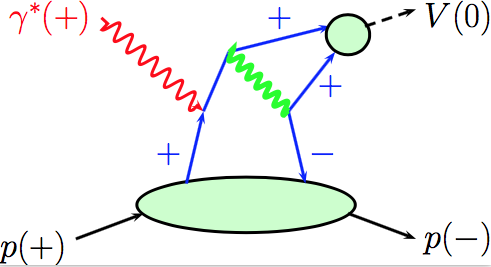
\includegraphics[width=0.4\textwidth]{figures/GK-handbag.png}
\caption{Schematic handbag description of hard exclusive meson electroproduction. The virtual photon interacts with a parton in the nucleon through a hard subprocess, while the nonperturbative nucleon structure is parametrized in terms of GPDs.}
\label{fig:handbag}
\end{figure}

Polarization observables provide information beyond that contained in the unpolarized cross section because they isolate different combinations and interferences of the underlying helicity amplitudes. In particular, the target-spin observables measured with a longitudinally polarized neutron target contain $\sin\phi$ and $\sin2\phi$ modulations that are sensitive to imaginary parts of interference terms, while the beam--target observables provide complementary sensitivity to helicity-dependent combinations of amplitudes and their real interference terms. These measurements can therefore constrain the relative sizes and phases of the longitudinal and transverse reaction amplitudes. The earlier CLAS6 measurement of exclusive $\pi^+$ production observed sizable target- and beam--target-spin asymmetries over a broad kinematic range and found that the available GPD-based calculation did not provide a complete description of the data~\cite{CLAS:2016dlz}. More recently, a multidimensional CLAS12 measurement of the beam-spin-dependent structure-function ratio $\sigma_{LT'}/\sigma_0$ in the proton $ep\rightarrow e^\prime n\pi^+$ channel demonstrated continued sensitivity to the transverse reaction mechanism in the CLAS12 kinematic regime~\cite{CLAS:2022iqy}.

The longitudinally polarized deuterated-ammonia target employed by CLAS12 Run Group C (RGC) makes it possible to extend these studies to target-spin and beam--target-spin observables with high statistics over a broad multidimensional kinematic range. Because the target polarization is defined along the incident electron beam rather than along the virtual-photon direction, the measured laboratory-frame target-spin observables also contain contributions from the component of the target polarization transverse to the virtual photon. These terms are suppressed by $\sin\theta_\gamma$, where $\theta_\gamma$ is the angle between the incident beam and virtual photon. Their treatment, and the distinction between the laboratory-frame amplitudes reported in this analysis and amplitudes defined with respect to the virtual-photon direction, are discussed in detail in the asymmetry-extraction section and the bound-neutron interpretation study.

For completeness, the principal kinematic quantities used throughout this analysis are defined here. The four-momentum transfer from the incident electron to the target is
\begin{equation}
    q = k-k^\prime,
\end{equation}
where $k$ and $k^\prime$ are the incident- and scattered-electron four-momenta. Its virtuality is
\begin{equation}
    Q^2=-q^2,
\end{equation}
and the Bjorken scaling variable is
\begin{equation}
    x_B=\frac{Q^2}{2p\cdot q},
\end{equation}
where $p$ is the initial neutron four-momentum, taken at rest for the reconstruction convention and modified by nuclear motion in the physical target. The invariant mass of the virtual-photon--neutron system is
\begin{equation}
    W^2=(p+q)^2,
\end{equation}
and the fractional electron energy loss in the target rest frame is
\begin{equation}
    y=\frac{p\cdot q}{p\cdot k}.
\end{equation}
The virtual-photon polarization parameter is
\begin{equation}
    \epsilon =
    \frac{1-y-\frac{1}{4}\gamma^2y^2}
         {1-y+\frac{1}{2}y^2+\frac{1}{4}\gamma^2y^2},
    \qquad
    \gamma=\frac{2m_n x_B}{Q}.
\end{equation}
The azimuthal angle $\phi$ is the angle between the lepton-scattering plane and the hadronic production plane, defined according to the Trento convention. The squared four-momentum transfer to the target is reconstructed from the virtual-photon and measured pion four-momenta as
\begin{equation}
t=(q-p_\pi)^2,
\end{equation}
where $p_\pi$ is the $\pi^-$ four-momentum. For the exclusive reaction $en\rightarrow e^\prime p\pi^-$, this is equivalent by four-momentum conservation to the baryonic definition $t=(p-p^\prime)^2$, where $p^\prime$ is the detected recoil-proton four-momentum. The distance from the forward kinematic limit is defined as
\begin{equation}
    t'=t-t_{\min}.
\end{equation}
Here $t_{\min}$ is the exact forward two-body kinematic limit for $\gamma^*n\rightarrow\pi^-p$. In the $\gamma^*n$ center-of-mass frame,
\begin{equation}
    t_{\min}
    =
    -Q^2+m_{\pi}^2
    -2E_{\gamma^*}^*E_{\pi}^*
    +2|\mathbf{q}^*||\mathbf{p}_{\pi}^*|,
\end{equation}
with
\begin{align}
    E_{\gamma^*}^* &= \frac{W^2-m_n^2-Q^2}{2W},
    &
    |\mathbf{q}^*| &= \frac{\lambda^{1/2}(W^2,-Q^2,m_n^2)}{2W},
    \\
    E_{\pi}^* &= \frac{W^2+m_{\pi}^2-m_p^2}{2W},
    &
    |\mathbf{p}_{\pi}^*| &= \frac{\lambda^{1/2}(W^2,m_{\pi}^2,m_p^2)}{2W},
\end{align}
where $\lambda(a,b,c)=a^2+b^2+c^2-2ab-2ac-2bc$. This exact definition, including the pion and recoil-proton masses, is used event by event throughout the analysis. Finally, exclusivity is characterized using the squared missing mass
\begin{equation}
    M_X^2=(k+p-k^\prime-p^\prime-p_\pi)^2,
\end{equation}
which is centered near zero in the stationary-neutron approximation for the exclusive $en\rightarrow e^\prime p\pi^-$ reaction.

The measurements presented here extend the available information on polarized exclusive $\pi^-$ electroproduction into the CLAS12 kinematic regime. Their detailed interpretation in terms of helicity amplitudes, GPDs and the reaction mechanisms discussed above, including comparison with phenomenological calculations, is left to the corresponding physics publication and subsequent theoretical studies. The purpose of this analysis note is to document the extraction, validation and systematic uncertainties of the measured beam-spin and laboratory-frame target-spin ratios for exclusive $en\rightarrow e^\prime p\pi^-$ production with CLAS12 RGC.

The neutron is embedded in deuterium, so the stationary-neutron kinematics are a reconstruction convention rather than a statement that Fermi motion or final-state interactions vanish. In the $e'p\pi^-$ sample the detected proton is the produced recoil baryon; the deuteron spectator and nuclear effects will be examined through exclusivity and background studies. ND$_3$ provides vector polarization of spin-one deuterons. The preliminary harmonic model neglects explicit tensor-polarization terms; their possible impact requires validation. Comparisons with the preliminary work of Brandon Manley and Shohini Bhattacharya will examine additional chiral-even transverse amplitudes, without claiming a model-independent GPD extraction.

\clearpage\section{Channel Selection}
\subsection{Data sets}
\begin{table}[htbp]
  \centering
  \sisetup{detect-all}
  \resizebox{\columnwidth}{!}{%
  \begin{tabular}{|l|l|l|c|c|c|l|l|}
    \hline
    \textbf{Period} & \textbf{Run Range} & \textbf{Beam Energy}
      & \textbf{FT} & \textbf{Torus} & \textbf{Solenoid}
      & \textbf{Coatjava Tracking} & \textbf{Beam Current}\\
    \hline
    RGB Sp19 & 6156--6603
      & \makecell[l]{\SI{10.5986}{\giga\electronvolt}\,(6156--6399)\\
          \SI{10.1998}{\giga\electronvolt}\,(6409--6603)}
      & On & $-1$ & $-1$ & 10.0.7 (no DAF) & \\
    \hline
    RGB Fa19 & 11093--11283 & \SI{10.4096}{\giga\electronvolt}
      & On & $+1$ & $-1$ & 10.0.7 (no DAF) & \\
    \hline
    RGB Sp20 & 11323--11571 & \SI{10.3894}{\giga\electronvolt}
      & On & $-1$ & $-1$ & 10.0.7 (no DAF) & \\
    \hline
    RGC Su22 & 16043--16772 & \SI{10.5473}{\giga\electronvolt}
      & On & $-1$ & $-1$ & 10.0.9 (no DAF) & \SI{4}{\nano\ampere}\\
    \hline
    RGC Fa22 & 16843--17408
      & \makecell[l]{\SI{10.5473}{\giga\electronvolt}\,(16843--17065)\\
          \SI{10.5563}{\giga\electronvolt}\,(17066--17408)}
      & Off & $-1$
      & \makecell[l]{$-1$\,(16843--17183)\\$+1$\,(17185--17408)}
      & 11.1.0 (DAF) & \SI{8}{\nano\ampere}\\
    \hline
    RGC Sp23 & 17477--17811
      & \makecell[l]{\SI{10.5563}{\giga\electronvolt}\,(17477--17724)\\
          \SI{10.5593}{\giga\electronvolt}\,(17725--17811)}
      & On & \makecell[l]{$-1$\,(17477--17768)\\$+1$\,(17769--17811)}
      & $-1$ & 11.1.0 (DAF) & \SI{4}{\nano\ampere}\\
    \hline
  \end{tabular}%
  }
  \caption{Summary of the RGB and RGC run periods. Only the inbending portion of RGC Sp23 is used in this analysis. RGB beam currents are left unspecified.}
  \label{tab:run_periods}
\end{table}

The polarized sample comprises the RGC Su22, Fa22 and Sp23 ND$_3$ data. Carbon, CH$_2$, empty-target and He-bath data are available for all three periods. CD$_2$ is available only in Sp23. Only inbending RGC data are used, while both Fa22 solenoid polarities are included.

The target-unpolarized sample comprises RGB spring 2019 and spring 2020 inbending liquid-D$_2$ data and the high-energy fall 2019 outbending liquid-D$_2$ data. The low-energy BAND-calibration data are not included. RGB retains its longitudinal beam polarization and has zero target polarization.

The selected final state consists of a forward-detector electron, a proton in the forward or central detector, and a forward-detector $\pi^-$. The detector and kinematic requirements are described below.

\subsection{Quality Assurance}
\label{sec::QADB}

The dead elements of CLAS12 (e.g. dead PMTs) are accounted for before the approved cooking of the data via the hardware status tables (c.f. \href{https://clasweb.jlab.org/wiki/images/8/8d/Statustables_RGCSummer2022review2024.pdf}{Su22}, \href{https://clasweb.jlab.org/wiki/images/archive/9/96/20240828040441%21Statustables_RGCFall2022review2024.pdf}{Fa22} and \href{https://clasweb.jlab.org/wiki/images/d/dd/Statustables_RGCWinter2023review2025.pdf}{Sp23} ready-for-cooking review HW status table summaries).

The \href{https://github.com/JeffersonLab/clas12-qadb}{CLAS12 Quality Assurance Database} (QADB) v3.4.1 is used for all three run periods in this analysis. The QADB is used on a time epoch basis with a series of cuts defined as ``defect bits'' used by the analyzers to remove unsatisfactory data. The defect bits used in this analysis are `TotalOutlier', `TerminalOutlier', `MarginalOutlier', `SectorLoss', `LowLiveTime', `ChargeHigh', `ChargeNegative', `ChargeUnknown', `PossiblyNoBeam' and `Misc.'. The misceallaneus defect bit is a stand in for otherwise uncharacterized issues and can be ignored on a run-by-run basis if the issue at hand does not effect the analysis. We have allowed ``misc'' bits on all empty target and helium-bath runs and for the runs 17179-17183, 17188, 17189 and 17252 which were marked with a defect bit purely because the RICH detector (which is not used in this analysis) was down. In addition to the QADB, the runs during the ``Hall-C bleedthrough'' period between runs 16600 and 16700 were removed after several analyses showed significant drops in efficiency during that period.



\subsection{Particle Identification}
The relaxed processing retains EventBuilder electron, proton and negative-pion candidates with raw electron momentum above 2~GeV. The offline selection requires finite necessary kinematics, all three fiducial selections, an FD pion, and an FD or CD proton, followed by the DIS and exclusivity cuts. The aggregate legacy processing cuts are not imposed in the offline selection. Consequently the relaxed sample is not identical to the earlier processing-level PID selection. The original scalar diagnostic fields remain available for selection and background studies.

\subsection{Momentum Corrections}
\label{sec:momentum_corrections}
\subsubsection{Electron Corrections}
Due to imperfections in alignment, magnetic field mapping and other software reconstruction related effects the reconstructed momenta of final state particles may differ slightly from the true momenta. This can most readily be seen in the position of certain missing mass peaks e.g. the missing neutron peak in our exclusive channel e'(n)$\pi^+$. The peak should appear at precisely 0.8828~GeV$^2$ but due to these imperfections can appear shifted. We perform momentum corrections in a two stage process, first by developing momentum corrections for the electron using the position of the proton mass in elastic events and then secondly developing corrections for the $\pi^+$ after applying those electron corrections and fixing the position of the missing neutron peak in e'(n)$\pi^+$ events. The kinematic range of the elastic events does not extend to the full phase space of the exclusive $\pi^+$ final state electrons but as will be shown extrapolations are reasonably stable and the correction appears safe even in these regions.

The elastic sample is taken from the gmn train. Data are divided into four periods: Su22, Fa22 solenoid-1, Fa22 solenoid+1 and Sp23. As an example of the need for momentum corrections the position of the elastic peak in each of the six FD sectors of CLAS12 is shown in Fig.~\ref{fig:su22_uncorrected_elastic_peak}. Several sectors show comparatively large deviations from the expected peak value of W = 0.938~GeV. Additionally, possible $\theta$ dependence can be considered (although compared to earlier run groups, the $\theta$ and $\phi$ dependence of the missing mass peaks seem markedly improved, probably due to improvements in the pass-2 DC alignment procedures) and is shown in Fig.~\ref{fig:fa22_uncorrected_theta_trends}.

\begin{figure}[htp]
\internallinenumbers
\begin{subfigure}[t]{0.99\textwidth}
\centering
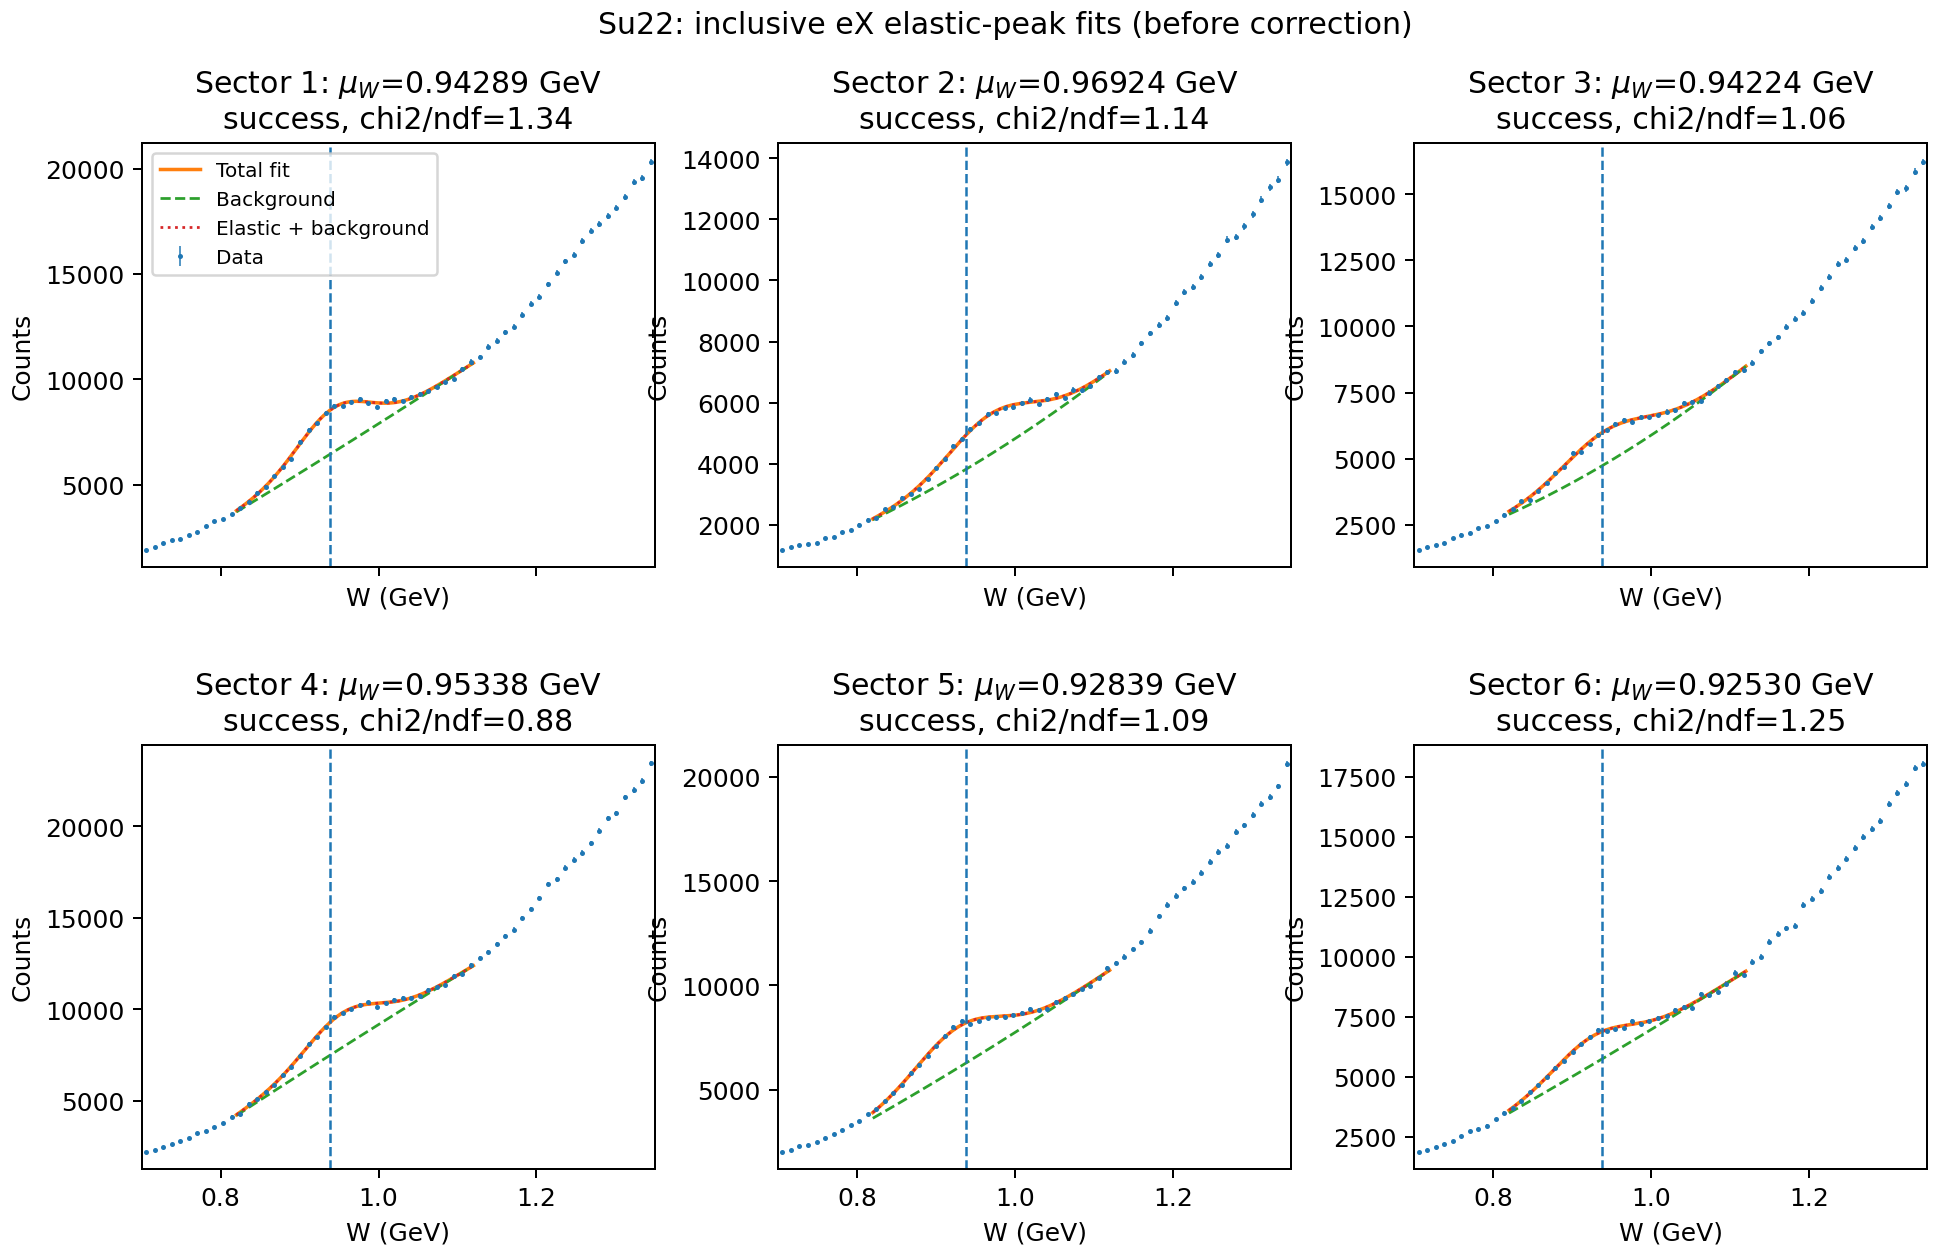
\includegraphics[width=\linewidth]{figures/channel_selection/momentum_corrections/electron/su22_integrated_w_by_sector.png}
\end{subfigure}
\caption{Elastic peak position in each of the six FD sectors of CLAS12 for Su22.} % Caption for the whole figure
\label{fig:su22_uncorrected_elastic_peak} % Label for referencing the entire figure
\end{figure}

\begin{figure}[htp]
\internallinenumbers
\begin{subfigure}[t]{0.99\textwidth}
\centering
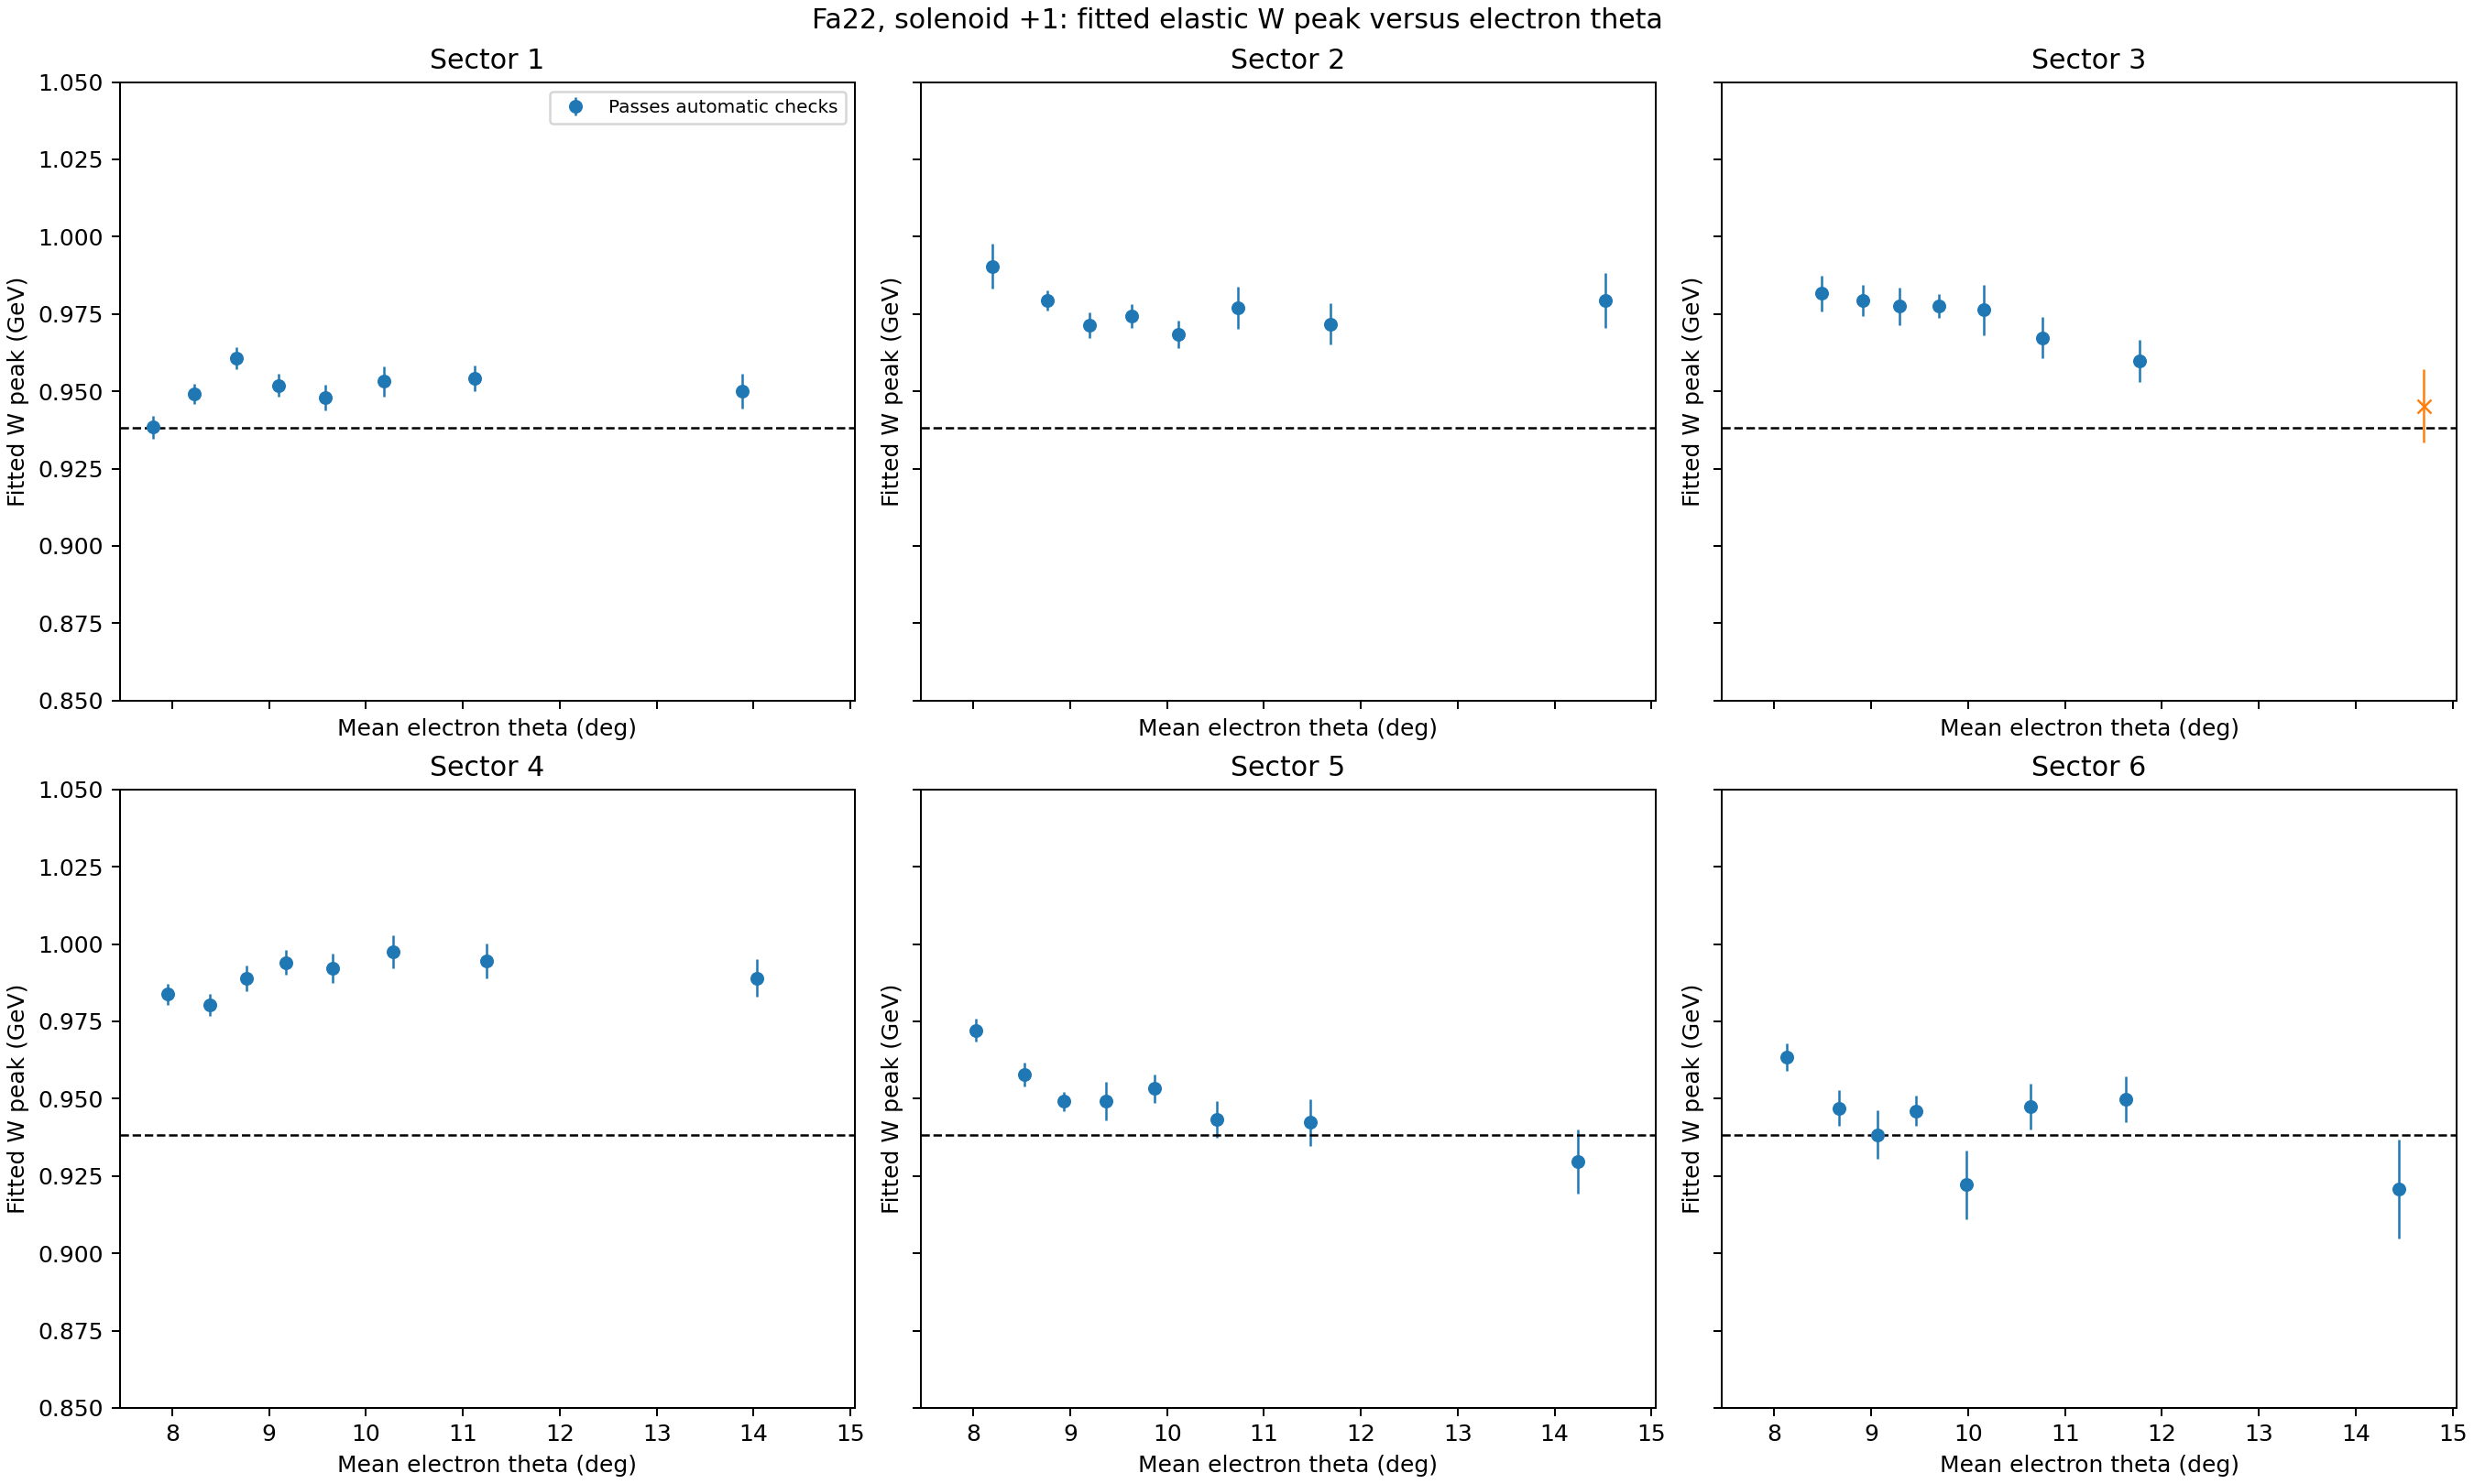
\includegraphics[width=\linewidth]{figures/channel_selection/momentum_corrections/electron/fa22_solenoid_plus_w_peak_vs_theta.png}
\end{subfigure}
\caption{Fitted elastic peak in each of the six FD sectors of CLAS12 as a function of $e_\theta$ for Fa22 solenoid-1.} % Caption for the whole figure
\label{fig:fa22_uncorrected_theta_trends}
\end{figure}

The $W$ spectrum is fit to a signal + background, $f(W) = S(W) + B(W)$ where the signal is a Gaussian,
\begin{align}
    S(W) = A e^{ \left[ - \frac{(W - \mu_W)^2}{2\sigma^2_W}\right]},
\end{align}
and the background is a simple quadratic polynomial,
\begin{align}
    B(W) = b_0 + b_1 W + b_2 W^2.
\end{align}
The measured momentum is assumed to differ from the true momentum by some small factor,
\begin{align}
    p_e^{\text{corr}} = (1+\delta) p_e,
\end{align}
with the $\delta$ fit to minimize the fitted elastic peak difference from the true elastic peak. The process is repeated in each $e_\theta$ bin and a simple polynomial is chosen for the $\delta(e_\theta)$,
\begin{align}
    \delta(e_\theta) = a_0 + a_1 e_\theta + a_2 e_\theta^2 + a_3 e_\theta^3 + ...
\end{align}
where the order of the polynomial is selected according to the Akaike Information Criterion (AIC) by requiring it to exceed 2 (to balance improved $\chi^2$ vs statistical fluctuations),
\begin{align}
    \text{AIC}_c = \chi^2 + 2k + \frac{2k(k+1)}{n-k-1},
\end{align}
where $n$ is the degree of the polynomial and $k$ is the number of fitted points. In general a linear function is preferred with a quadratic being used in some cases. An example of these fits can be seen in Fig.~\ref{fig:fa22_fitted_theta_trends}.

\begin{figure}[htp]
\internallinenumbers
\begin{subfigure}[t]{0.99\textwidth}
\centering
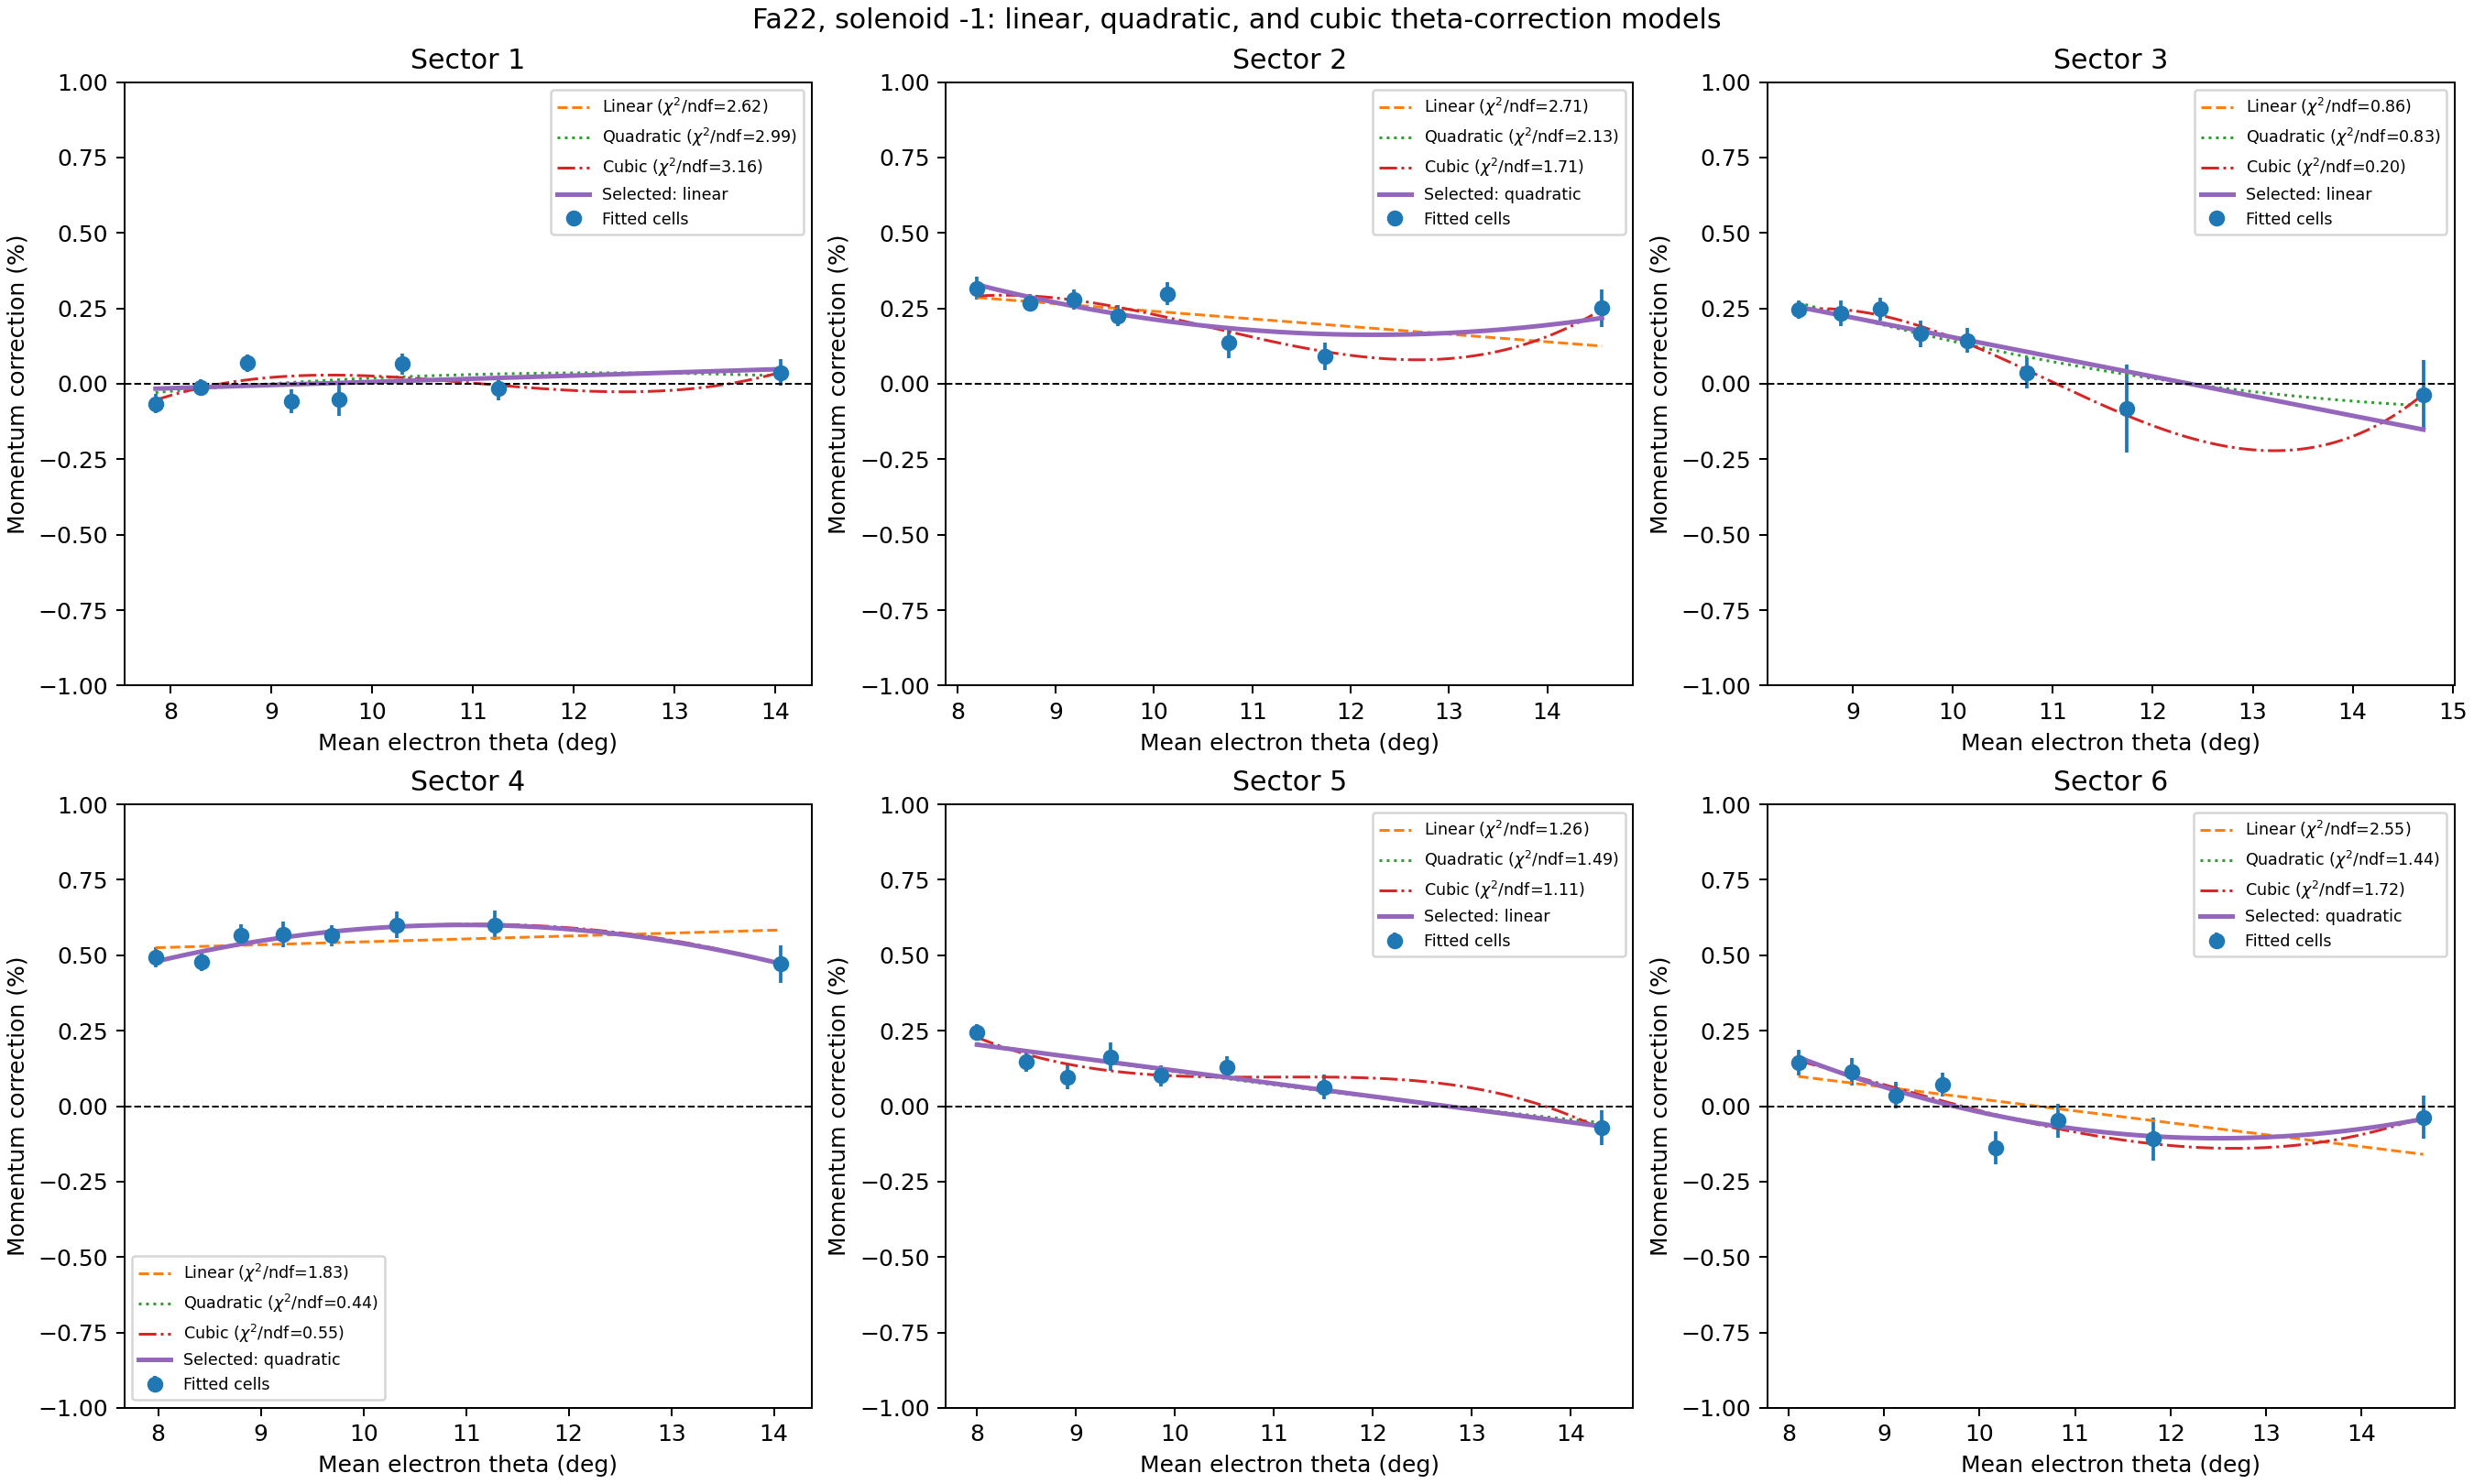
\includegraphics[width=\linewidth]{figures/channel_selection/momentum_corrections/electron/fa22_solenoid_minus_theta_model_selection.png}
\end{subfigure}
\caption{Fitted momentum correction function for the electron in each of the six FD sectors of CLAS12 as a function of $e_\theta$ for Fa22 solenoid-1.} % Caption for the whole figure
\label{fig:fa22_fitted_theta_trends}
\end{figure}

The fitted functions are presented in Tables~\ref{tab:Su22_electron_momentum_corrections}-\ref{fig:su22_integrated_before_and_after} and summary plots showing the effect of the corrections are shown in Figs.~\ref{fig:su22_integrated_before_and_after}-\ref{fig:sp23_theta_before_and_after}

\begin{table}[htbp]
\centering
\begin{tabular}{cl}
\toprule
Sector & $\delta(\theta_e)$ \\
\midrule
1 & $-0.003276 + 3.9818\times10^{-4}\theta_e$ \\
2 & $\phantom{-}0.004490 - 1.4350\times10^{-4}\theta_e$ \\
3 & $\phantom{-}0.004677 - 4.2114\times10^{-4}\theta_e$ \\
4 & $\phantom{-}0.002444 - 9.3691\times10^{-5}\theta_e$ \\
5 & $\phantom{-}0.001267 - 2.2314\times10^{-4}\theta_e$ \\
6 & $-0.001890 + 6.3591\times10^{-5}\theta_e$ \\
\bottomrule
\end{tabular}
\caption{Electron momentum correction functions for the Su22 data set. The corrected electron momentum is given by
$p_e^{\rm corr}=[1+\delta(\theta_e)]p_e$, where $\theta_e$ is in degrees. Corrections are derived for $8 < e_\theta < 15$~degrees. Tracks outside those ranges should use $\delta(8)$ or $\delta(15)$ respectively.}
\label{tab:Su22_electron_momentum_corrections}
\end{table}

\begin{table}[htbp]
\centering
\begin{tabular}{cl}
\toprule
Sector & $\delta(\theta_e)$ \\
\midrule
1 & $\phantom{-}1.9971\times10^{-4} + 1.0813\times10^{-4}\theta_e$ \\
2 & $\phantom{-}0.004853 - 1.1926\times10^{-4}\theta_e$ \\
3 & $\phantom{-}0.009825 - 6.3016\times10^{-4}\theta_e$ \\
4 & $\phantom{-}0.003173 + 2.0016\times10^{-4}\theta_e$ \\
5 & $\phantom{-}0.007813 - 6.7382\times10^{-4}\theta_e$ \\
6 & $\phantom{-}0.005404 - 4.6323\times10^{-4}\theta_e$ \\
\bottomrule
\end{tabular}
\caption{Electron momentum correction functions for the Fa22 solenoid-1 data set. Corrections are derived for $8 < e_\theta < 15$~degrees. Tracks outside those ranges should use $\delta(8)$ or $\delta(15)$ respectively.}
\label{tab:Fa22-1_electron_momentum_corrections}
\end{table}

\begin{table}[htbp]
\centering
\begin{tabular}{cl}
\toprule
Sector & $\delta(\theta_e)$ \\
\midrule
1 & $-9.8063\times10^{-4} + 1.0435\times10^{-4}\theta_e$ \\
2 & $\phantom{-}0.016937 - 0.002505\,\theta_e + 1.0245\times10^{-4}\theta_e^2$ \\
3 & $\phantom{-}0.008040 - 6.4998\times10^{-4}\theta_e$ \\
4 & $-0.010207 + 0.002954\,\theta_e - 1.3456\times10^{-4}\theta_e^2$ \\
5 & $\phantom{-}0.005466 - 4.2851\times10^{-4}\theta_e$ \\
6 & $\phantom{-}0.020615 - 0.003468\,\theta_e + 1.3870\times10^{-4}\theta_e^2$ \\
\bottomrule
\end{tabular}
\caption{Electron momentum correction functions for the Fa22 solenoid+1 data set. Corrections are derived for $8 < e_\theta < 15$~degrees. Tracks outside those ranges should use $\delta(8)$ or $\delta(15)$ respectively.}
\label{tab:Fa22+1_electron_momentum_corrections}
\end{table}

\begin{table}[htbp]
\centering
\begin{tabular}{cl}
\toprule
Sector & $\delta(\theta_e)$\\
\midrule
1 & $-0.017000 + 0.003460\,\theta_e - 1.6146\times10^{-4}\theta_e^2$ \\
2 & $\phantom{-}0.009163 - 4.5048\times10^{-4}\theta_e$ \\
3 & $\phantom{-}0.014589 - 0.001394\,\theta_e$ \\
4 & $\phantom{-}0.004071 - 3.5391\times10^{-4}\theta_e$ \\
5 & $\phantom{-}0.003038 - 5.0218\times10^{-4}\theta_e$ \\
6 & $\phantom{-}0.003121 - 3.6366\times10^{-4}\theta_e$ \\
\bottomrule
\end{tabular}
\caption{Electron momentum correction functions for the Sp23 data set. Corrections are derived for $8 < e_\theta < 15$~degrees. Tracks outside those ranges should use $\delta(8)$ or $\delta(15)$ respectively.}
\label{tab:Sp23_electron_momentum_corrections}
\end{table}  

\begin{figure}[htp]
\internallinenumbers
\begin{subfigure}[t]{0.99\textwidth}
\centering
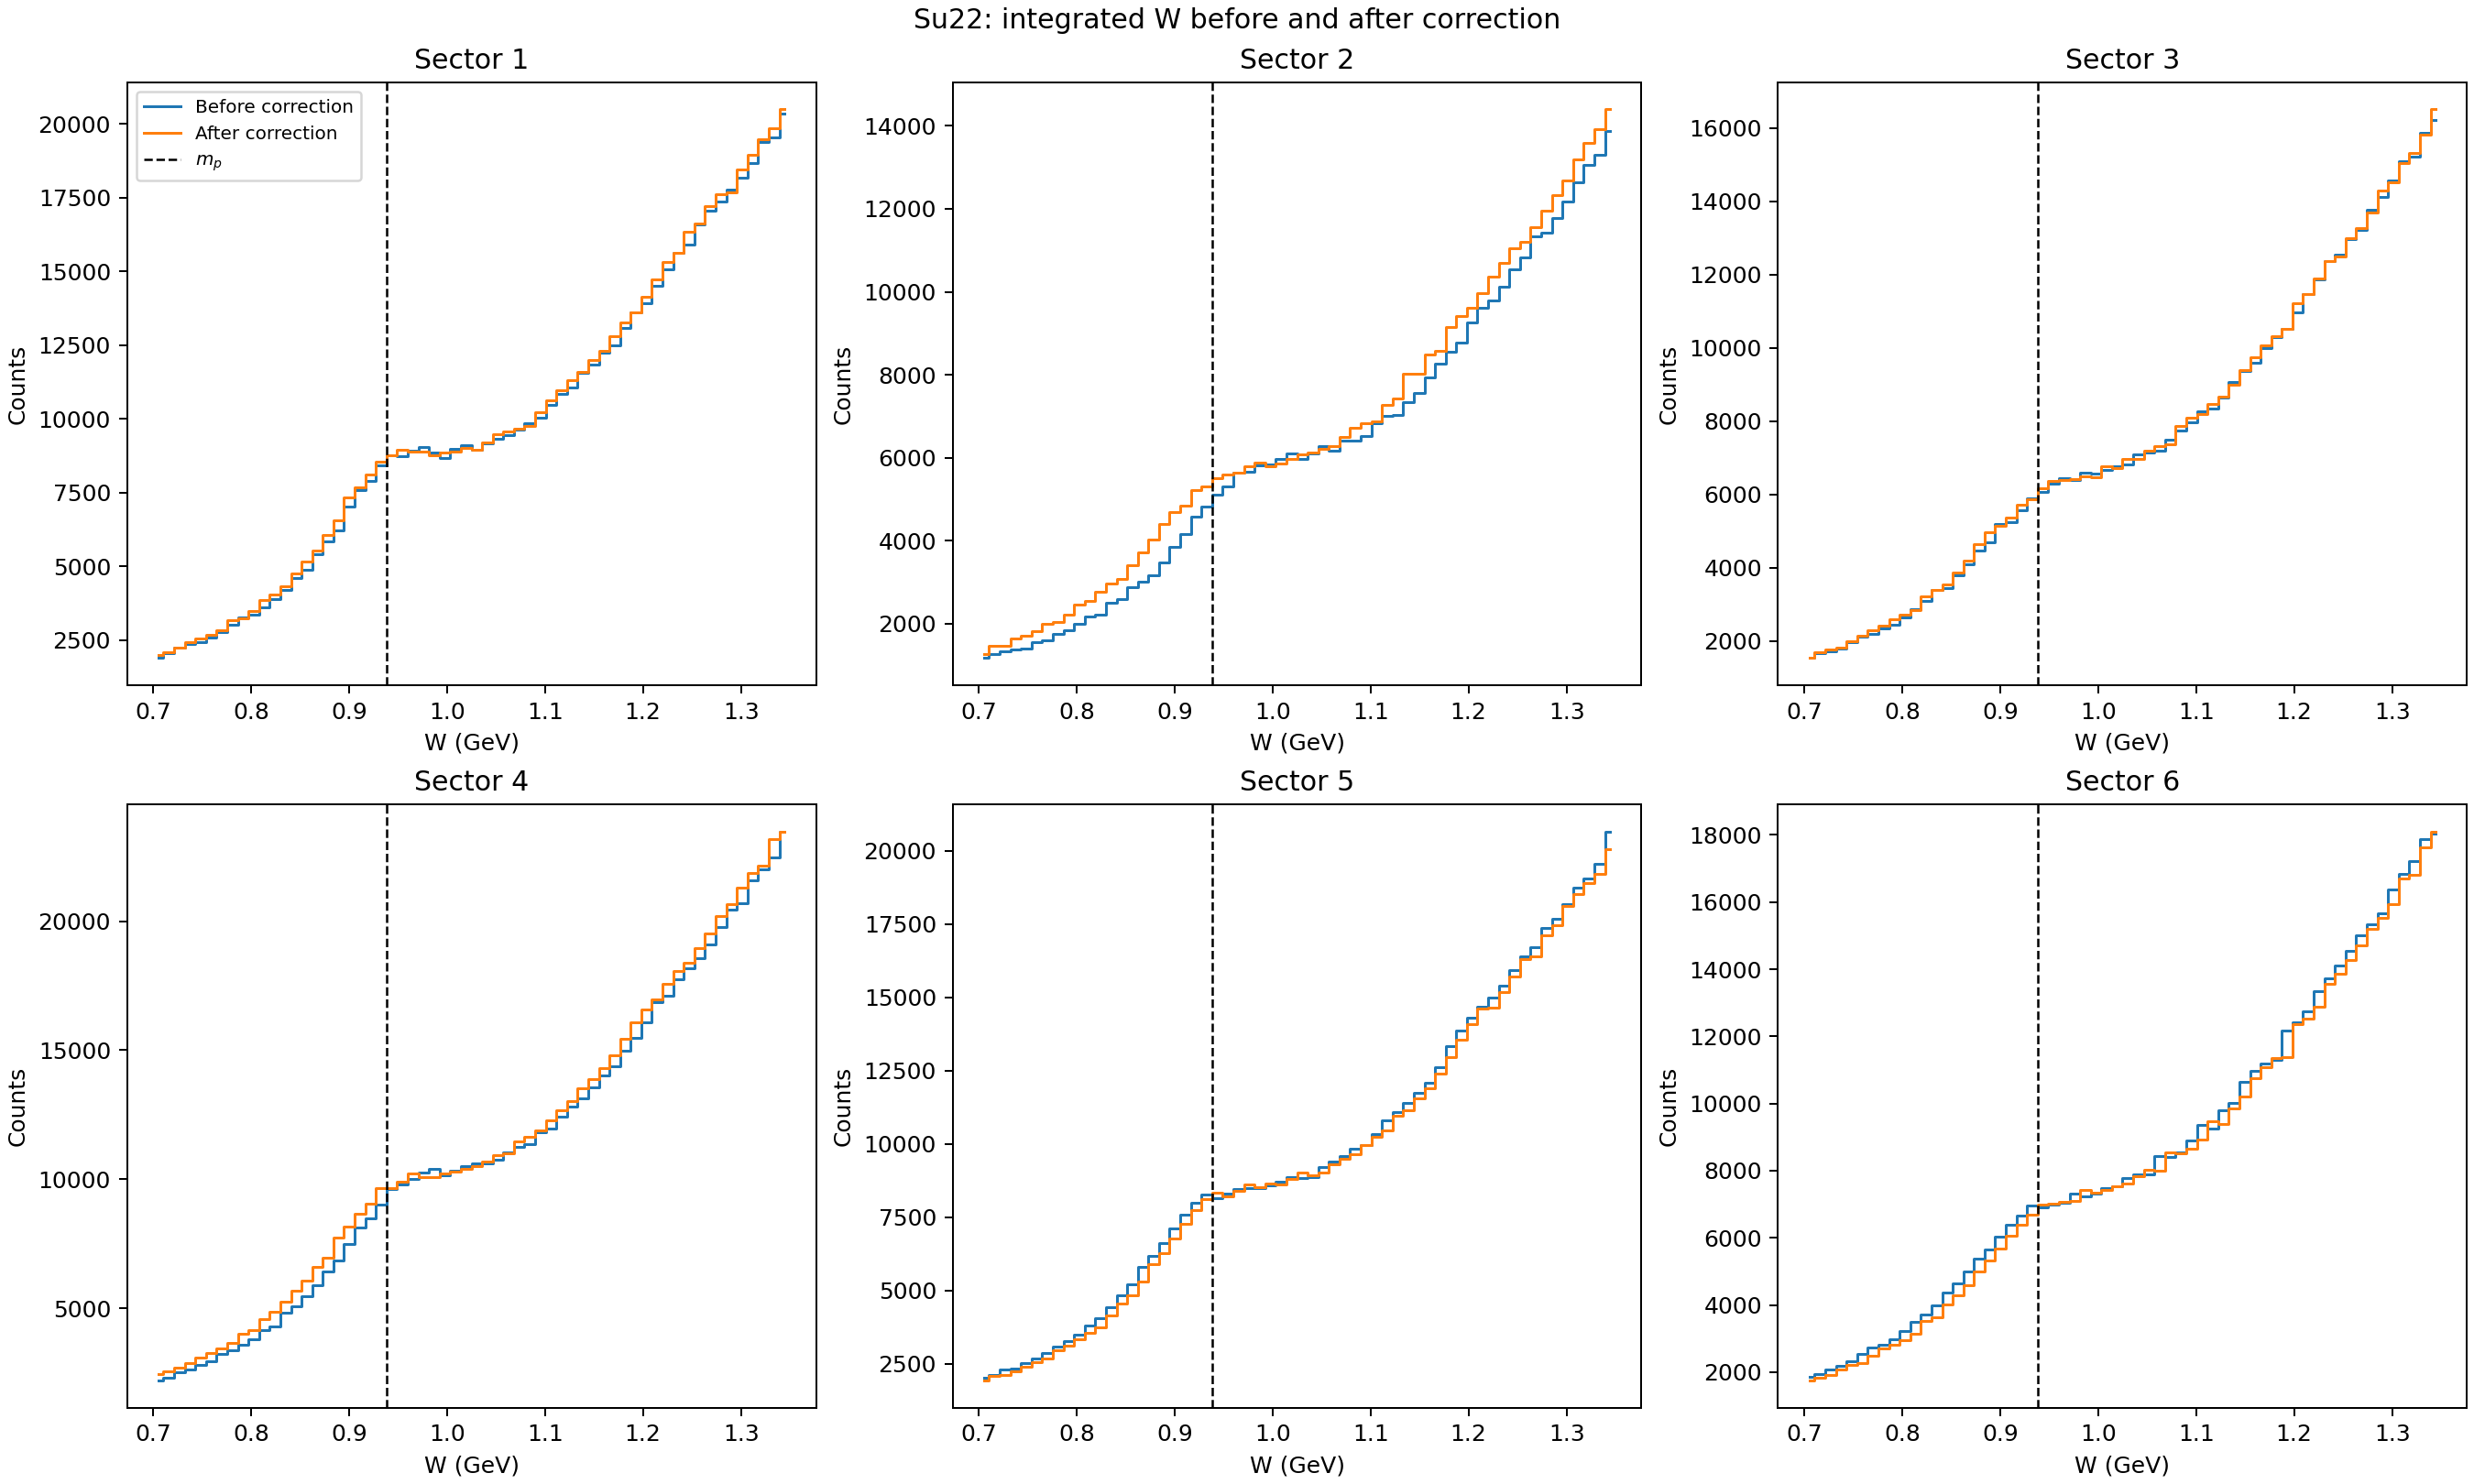
\includegraphics[width=\linewidth]{figures/channel_selection/momentum_corrections/electron/su22_integrated_w_before_after.png}
\end{subfigure}
\caption{Fitted elastic peak position before and after momentum corrections for each of the six sectors of CLAS12 for Su22.} % Caption for the whole figure
\label{fig:su22_integrated_before_and_after}
\end{figure}


\begin{figure}[htp]
\internallinenumbers
\begin{subfigure}[t]{0.99\textwidth}
\centering
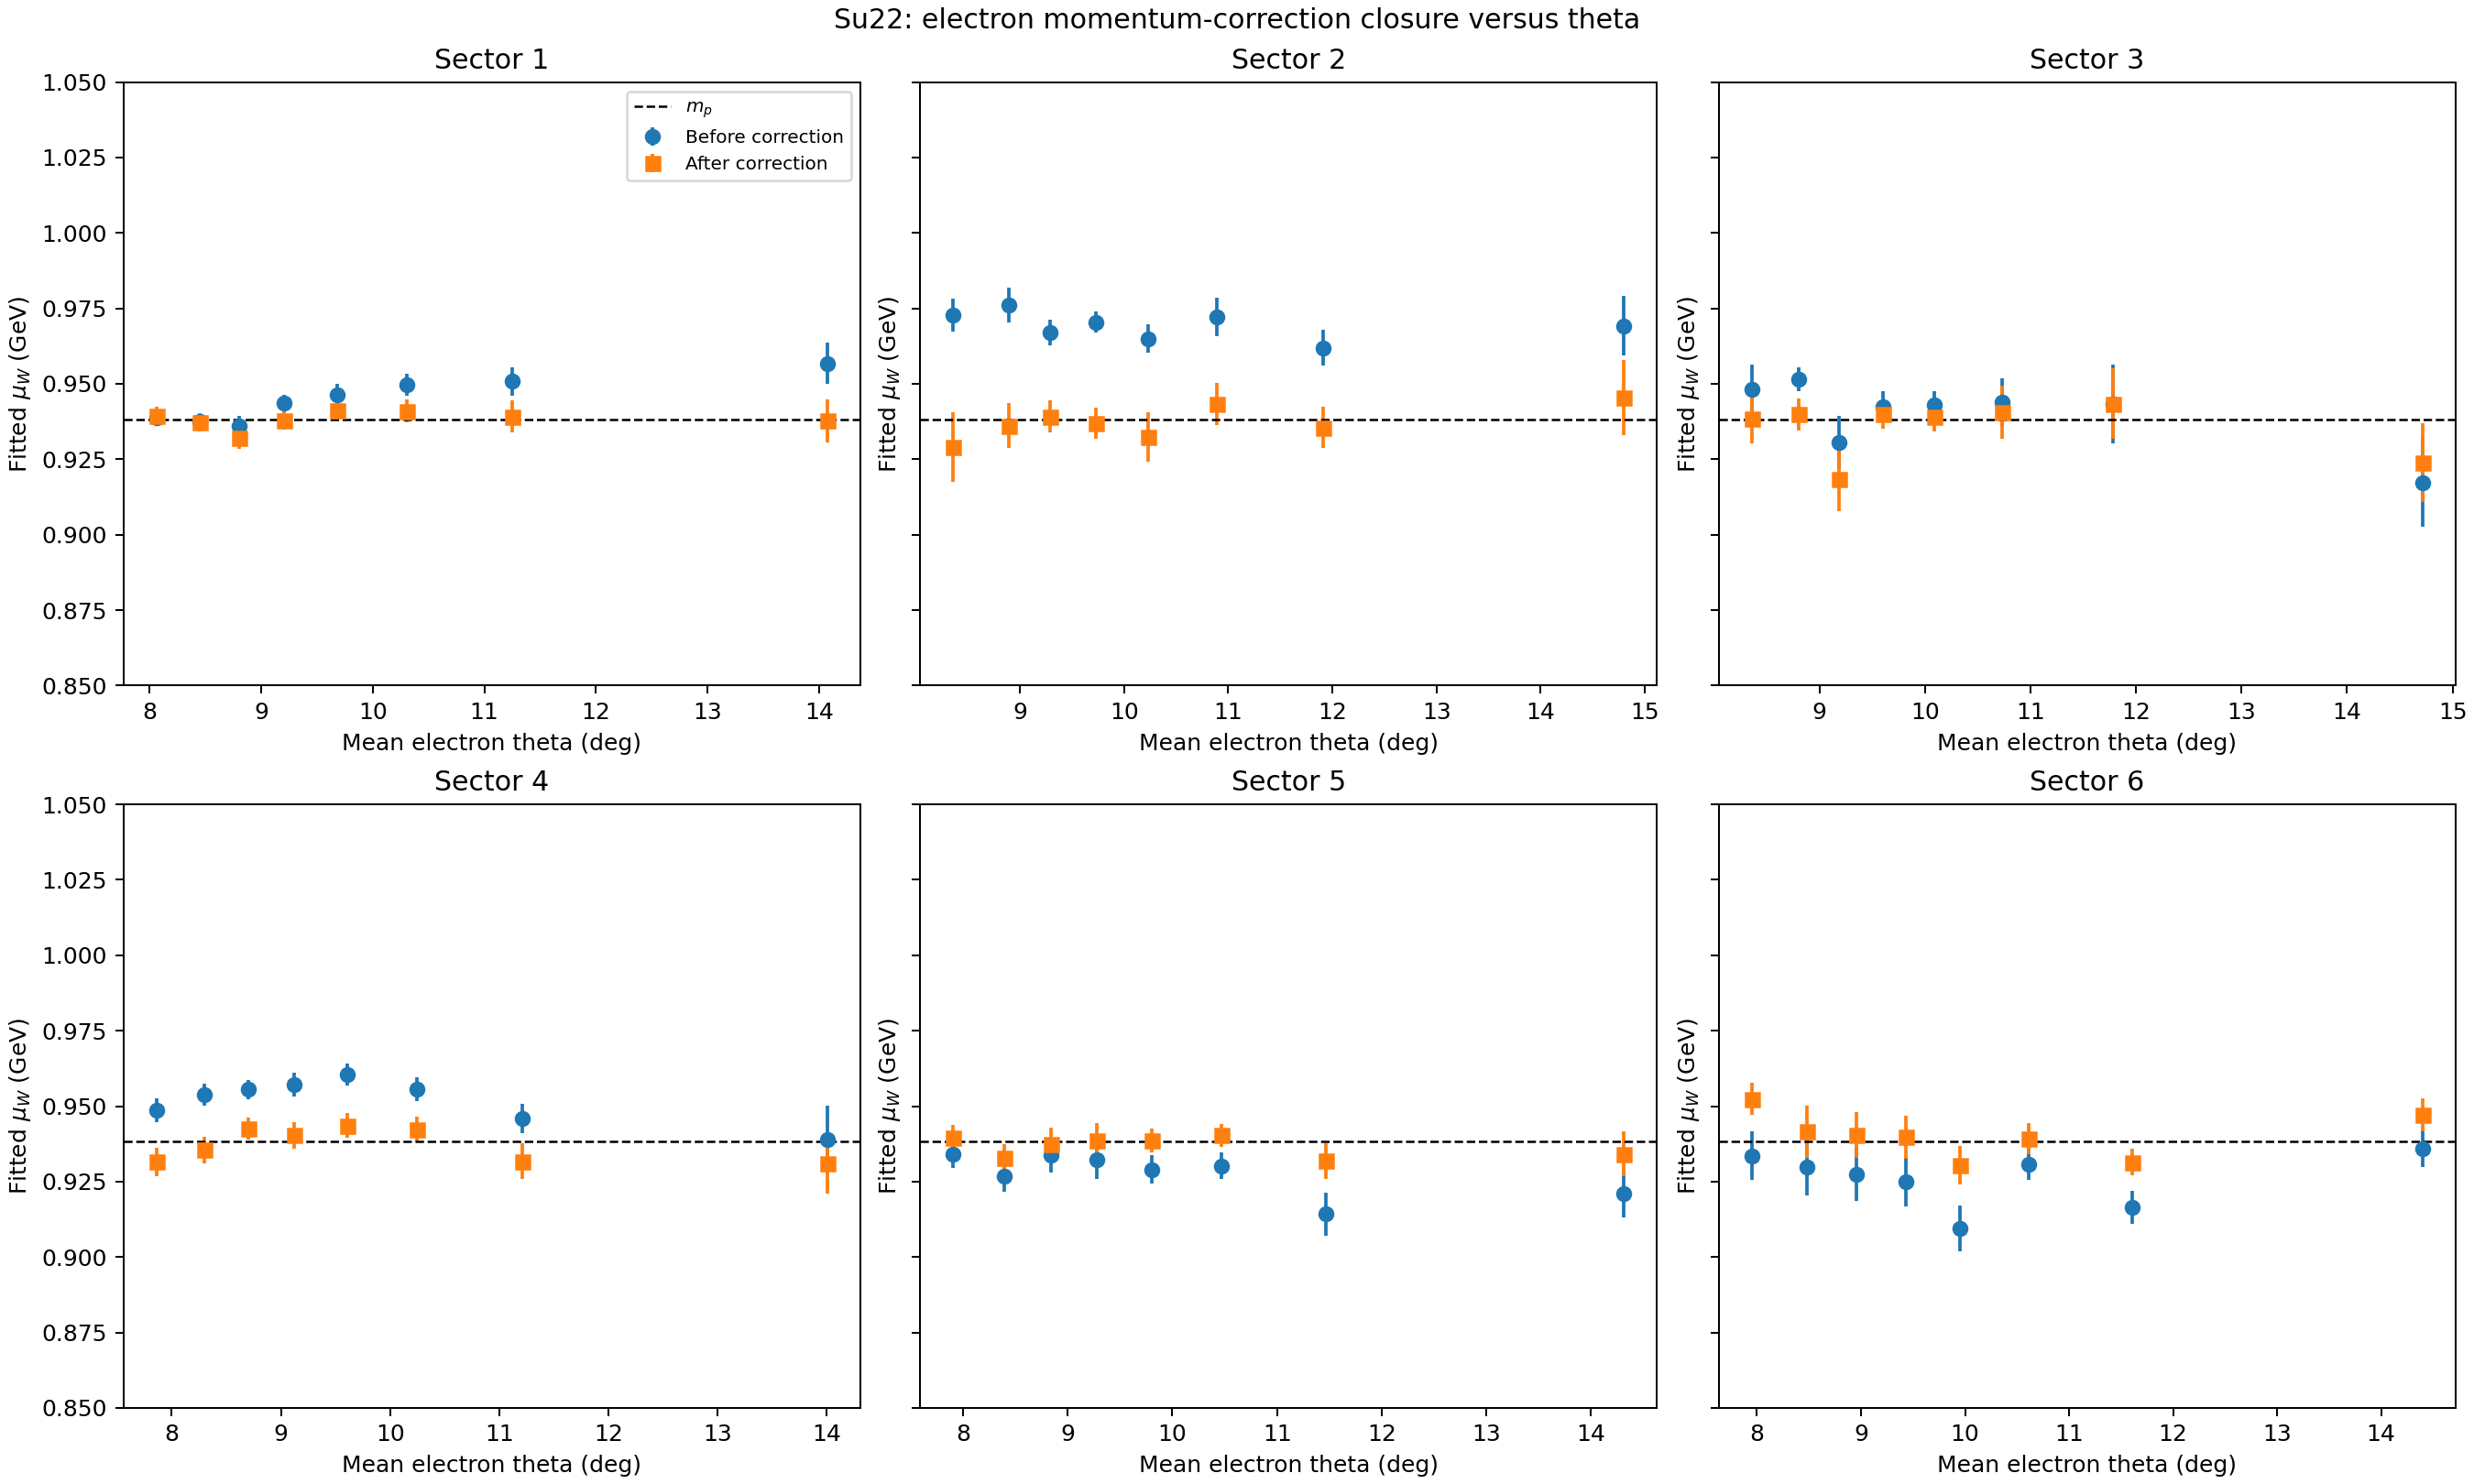
\includegraphics[width=\linewidth]{figures/channel_selection/momentum_corrections/electron/su22_theta_closure.png}
\end{subfigure}
\caption{Fitted elastic peak position before and after momentum corrections for each of the six sectors of CLAS12 for Su22 as a function of $e_\theta$} % Caption for the whole figure
\label{fig:su22_theta_before_and_after}
\end{figure}

\begin{figure}[htp]
\internallinenumbers
\begin{subfigure}[t]{0.99\textwidth}
\centering
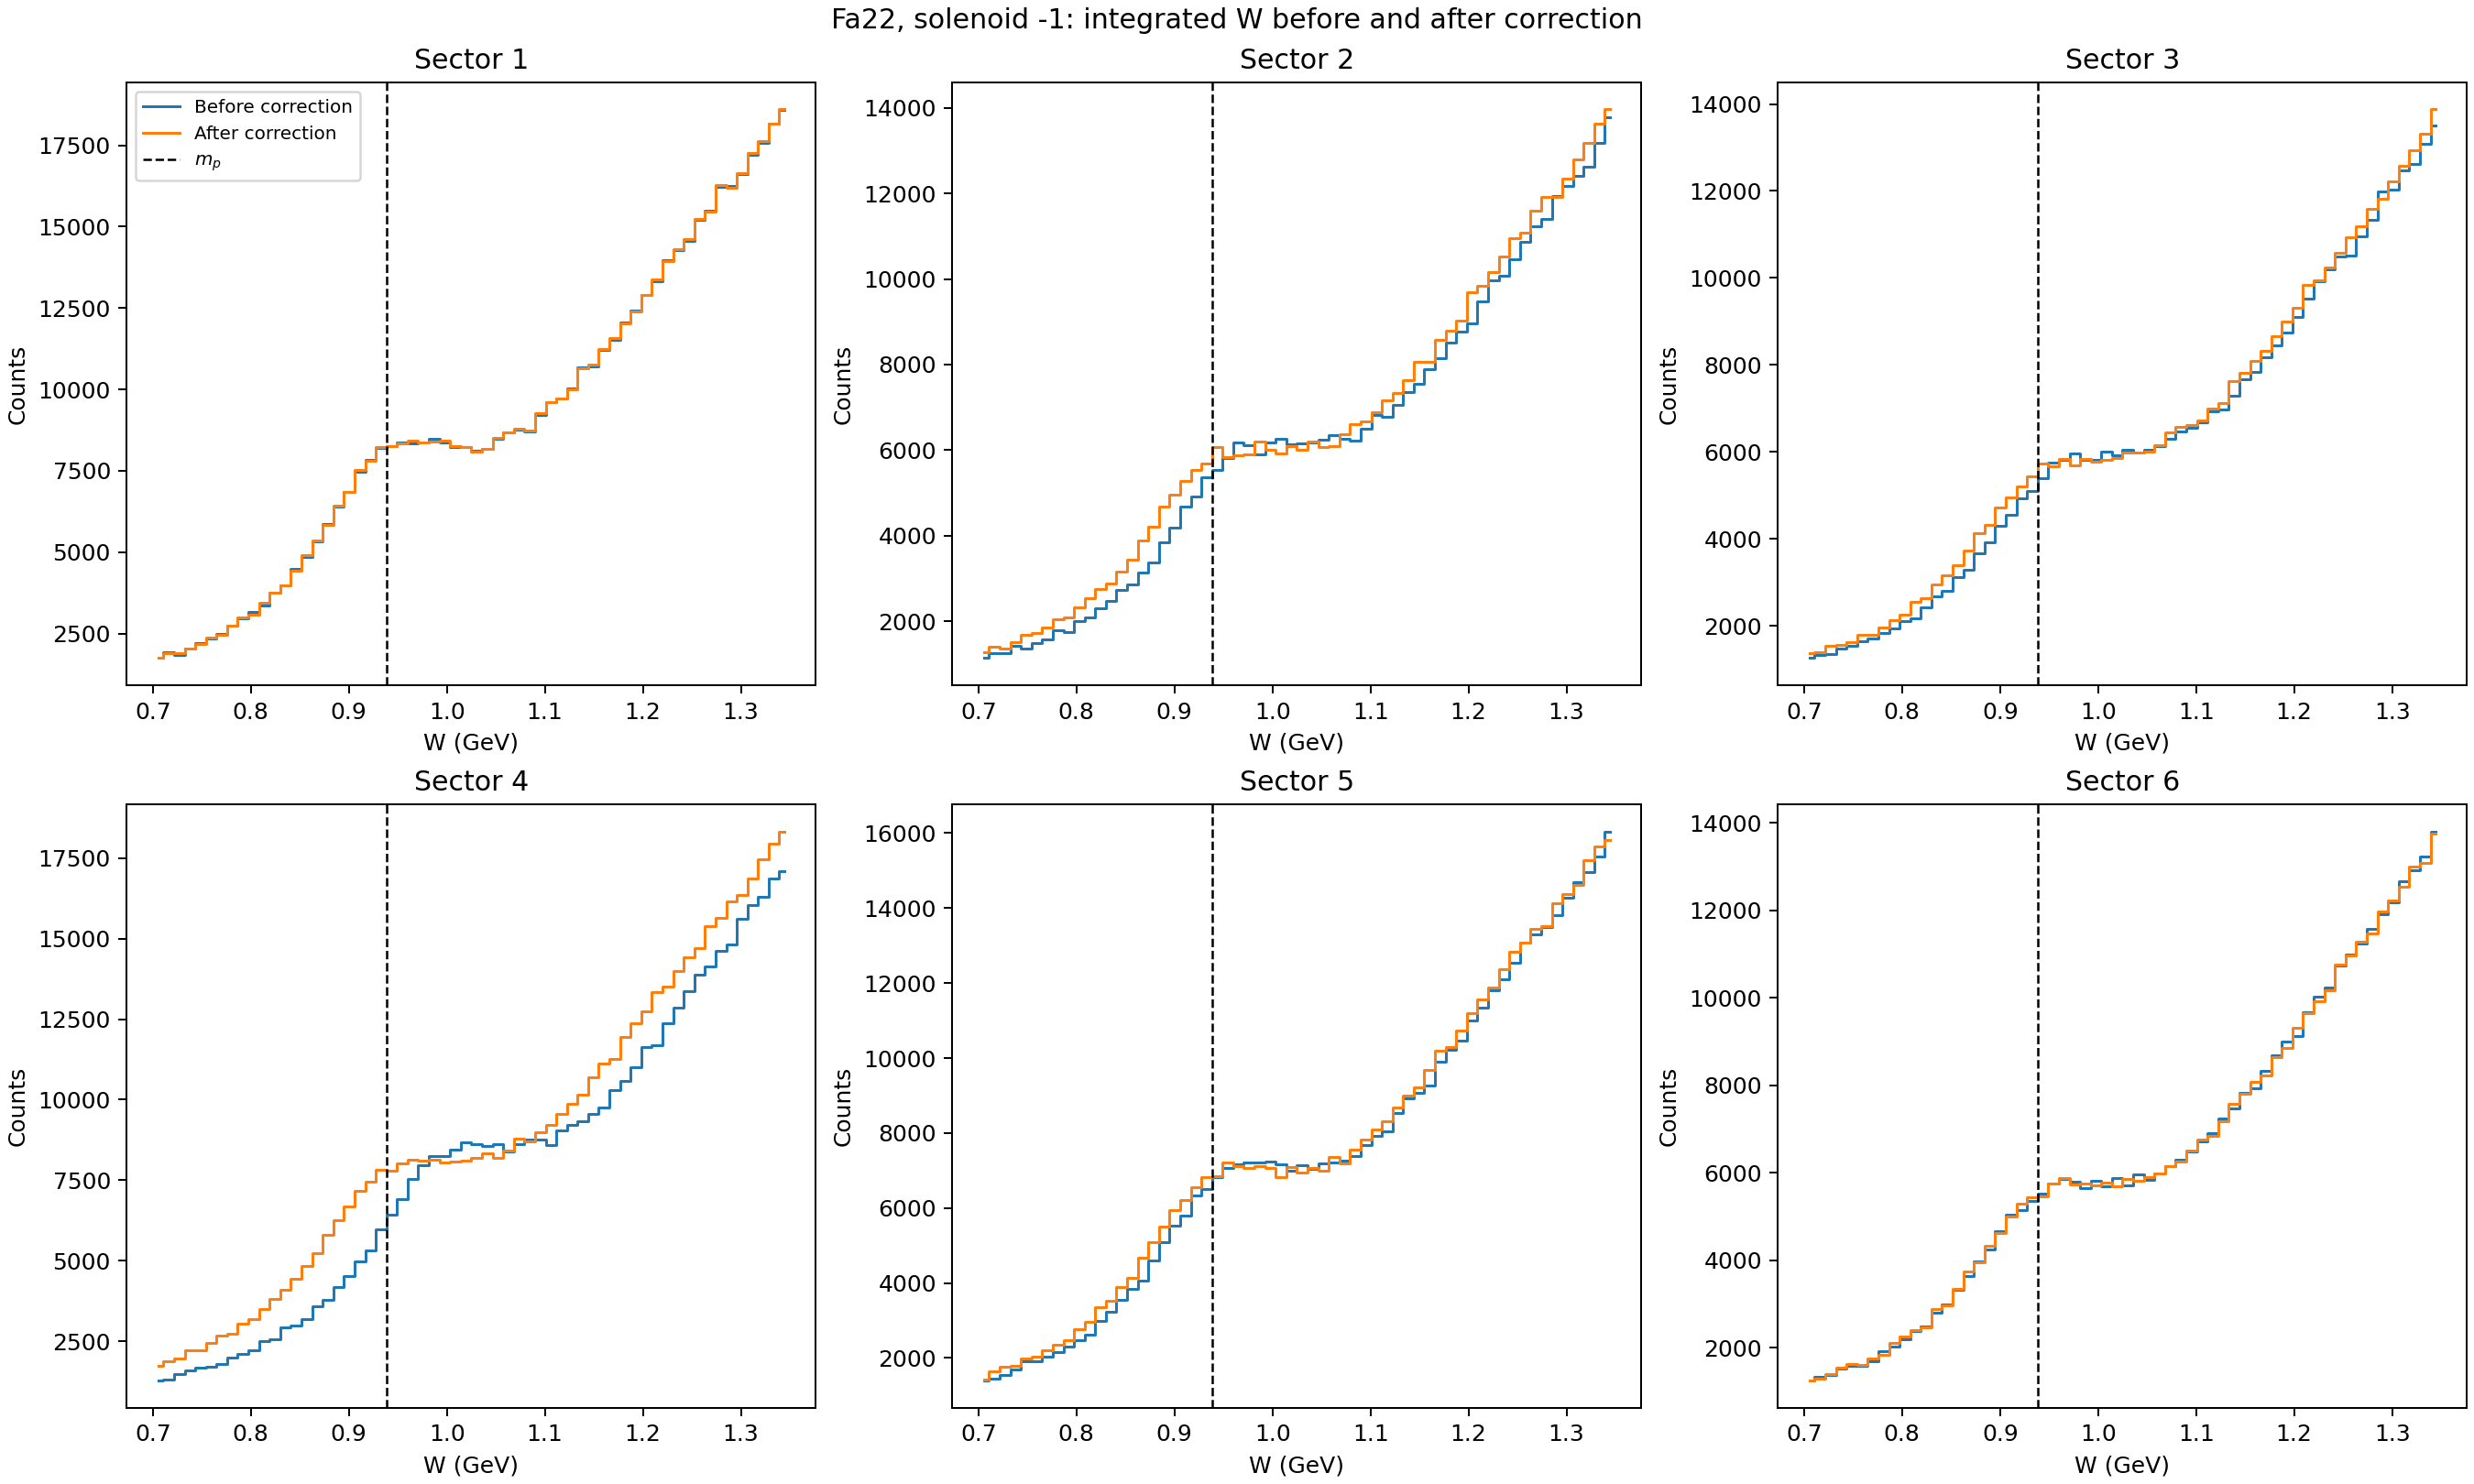
\includegraphics[width=\linewidth]{figures/channel_selection/momentum_corrections/electron/fa22_solenoid_minus_integrated_w_before_after.png}
\end{subfigure}
\caption{Fitted elastic peak position before and after momentum corrections for each of the six sectors of CLAS12 for Fa22 solenoid-1.} % Caption for the whole figure
\label{fig:fa22-1_integrated_before_and_after}
\end{figure}


\begin{figure}[htp]
\internallinenumbers
\begin{subfigure}[t]{0.99\textwidth}
\centering
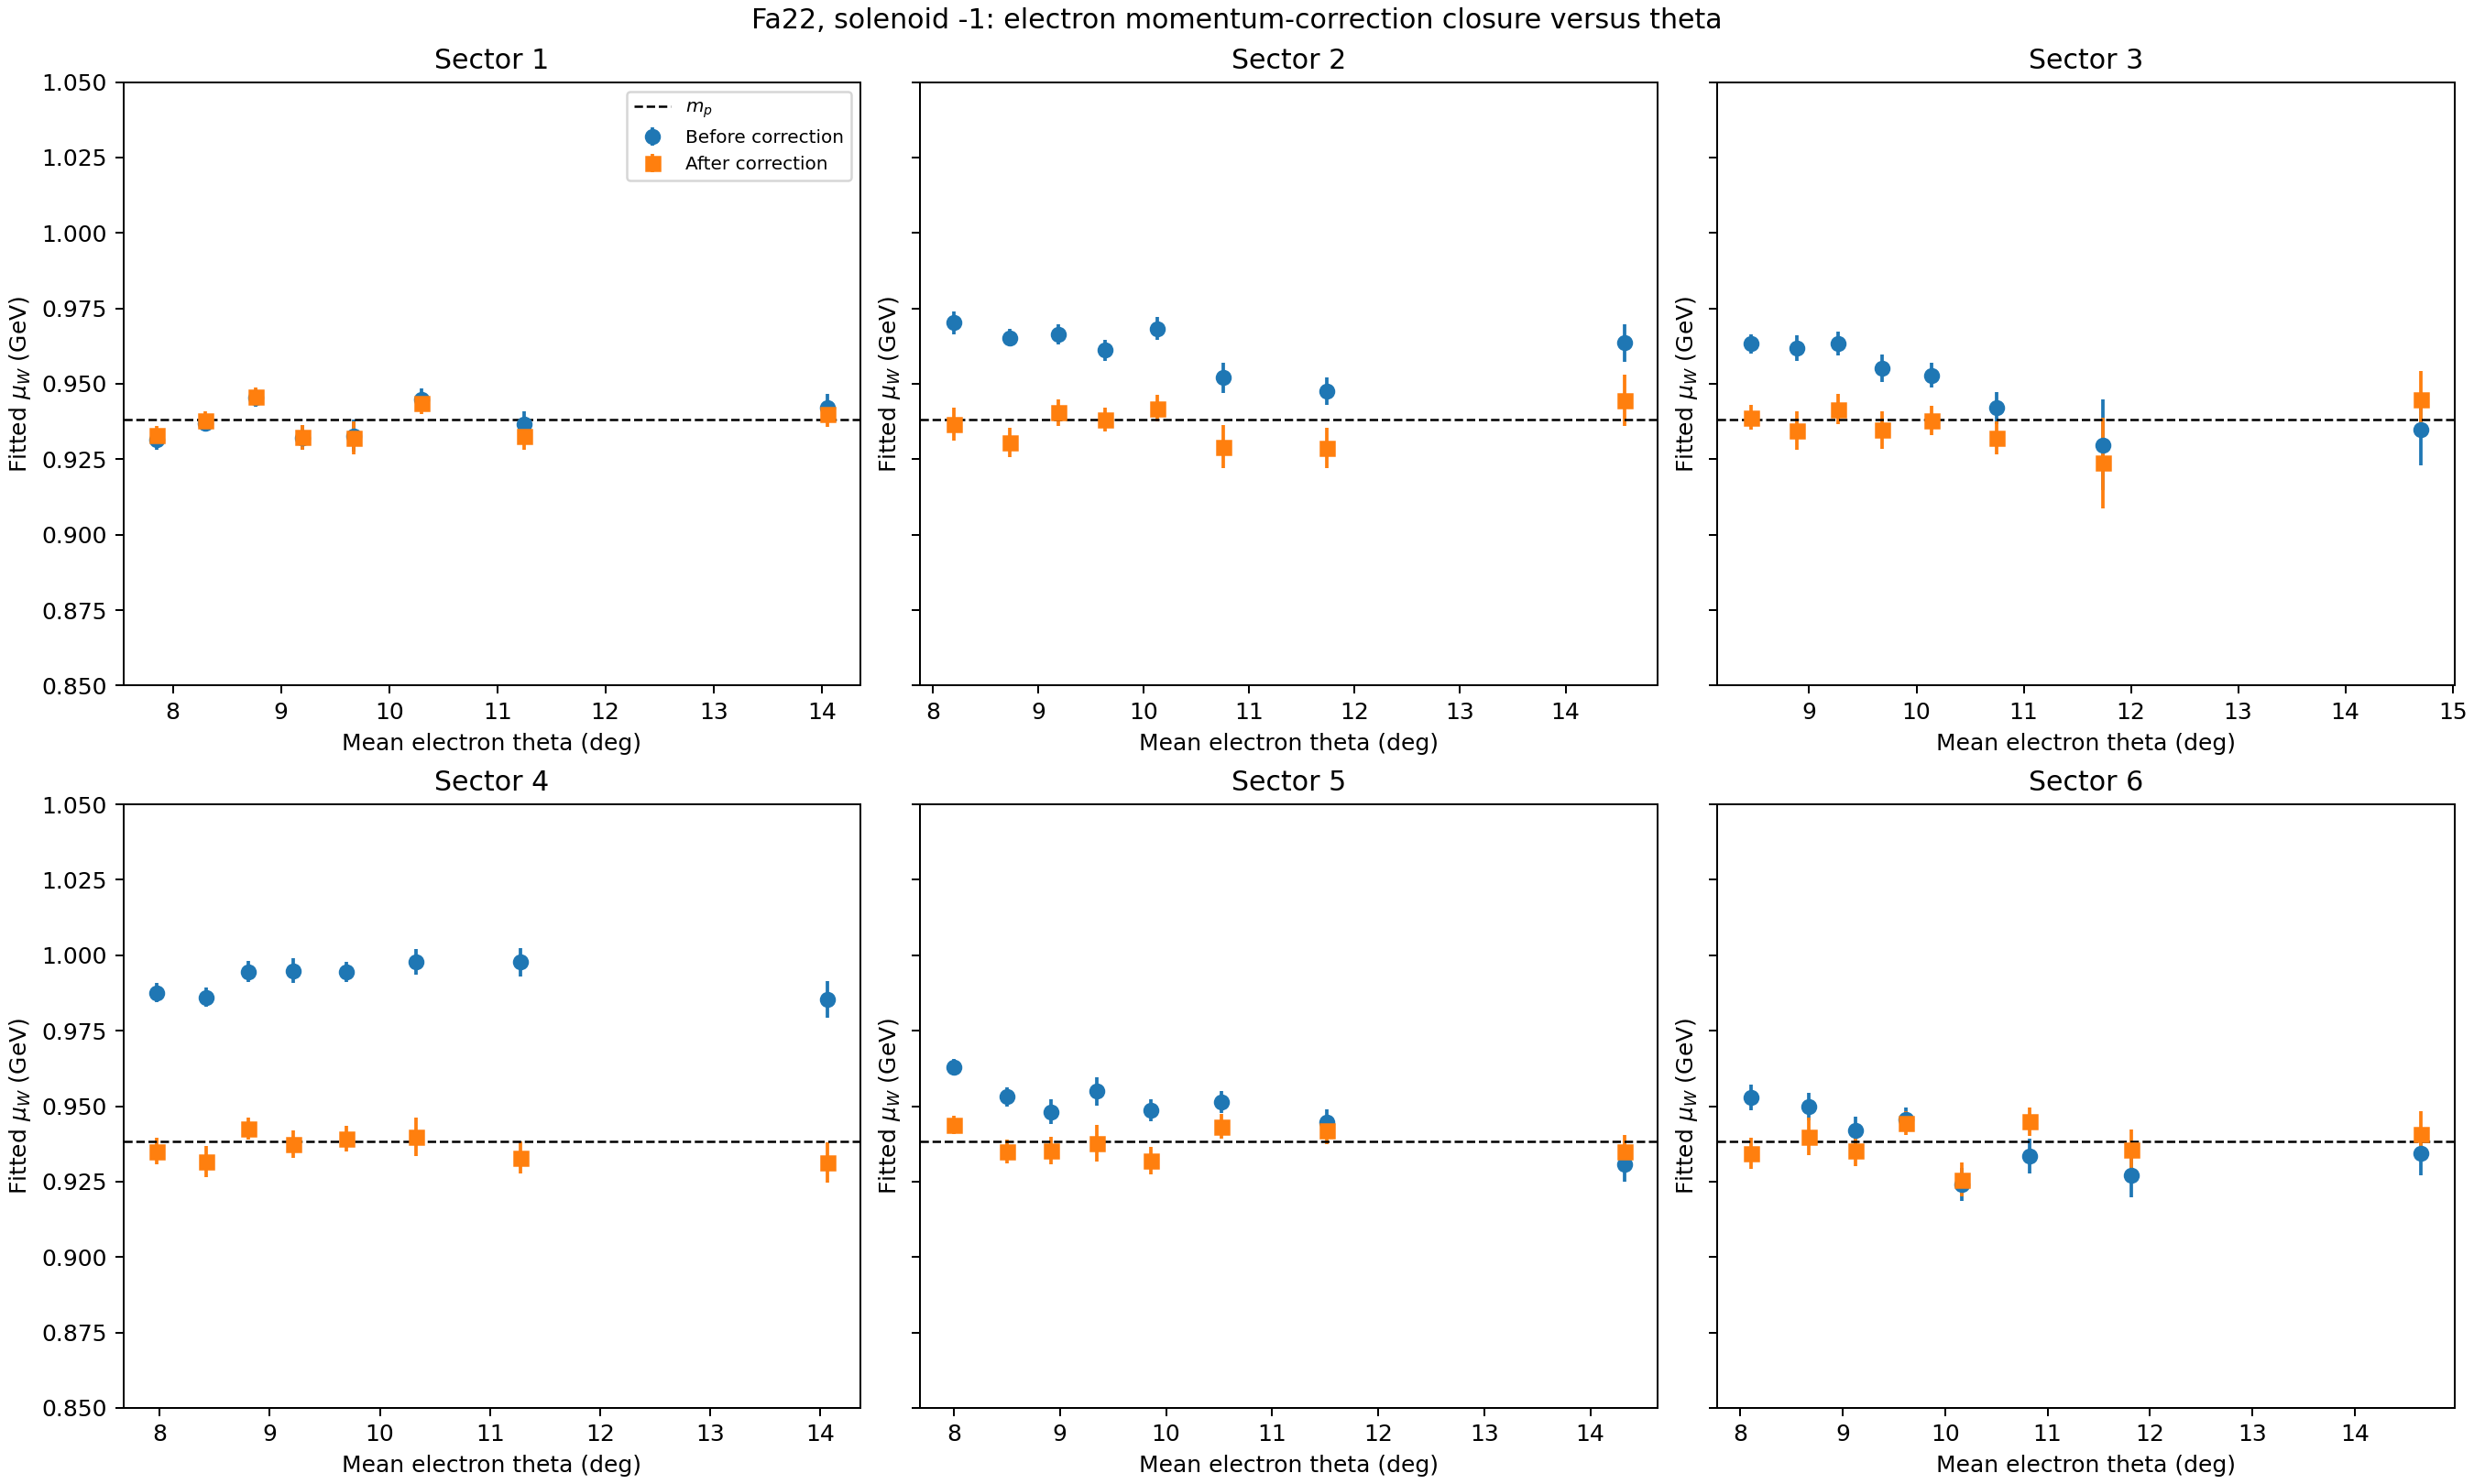
\includegraphics[width=\linewidth]{figures/channel_selection/momentum_corrections/electron/fa22_solenoid_minus_theta_closure.png}
\end{subfigure}
\caption{Fitted elastic peak position before and after momentum corrections for each of the six sectors of CLAS12 for Fa22 solenoid-1 as a function of $e_\theta$} % Caption for the whole figure
\label{fig:fa22_minus_solenoid_theta_before_and_after}
\end{figure}



\begin{figure}[htp]
\internallinenumbers
\begin{subfigure}[t]{0.99\textwidth}
\centering
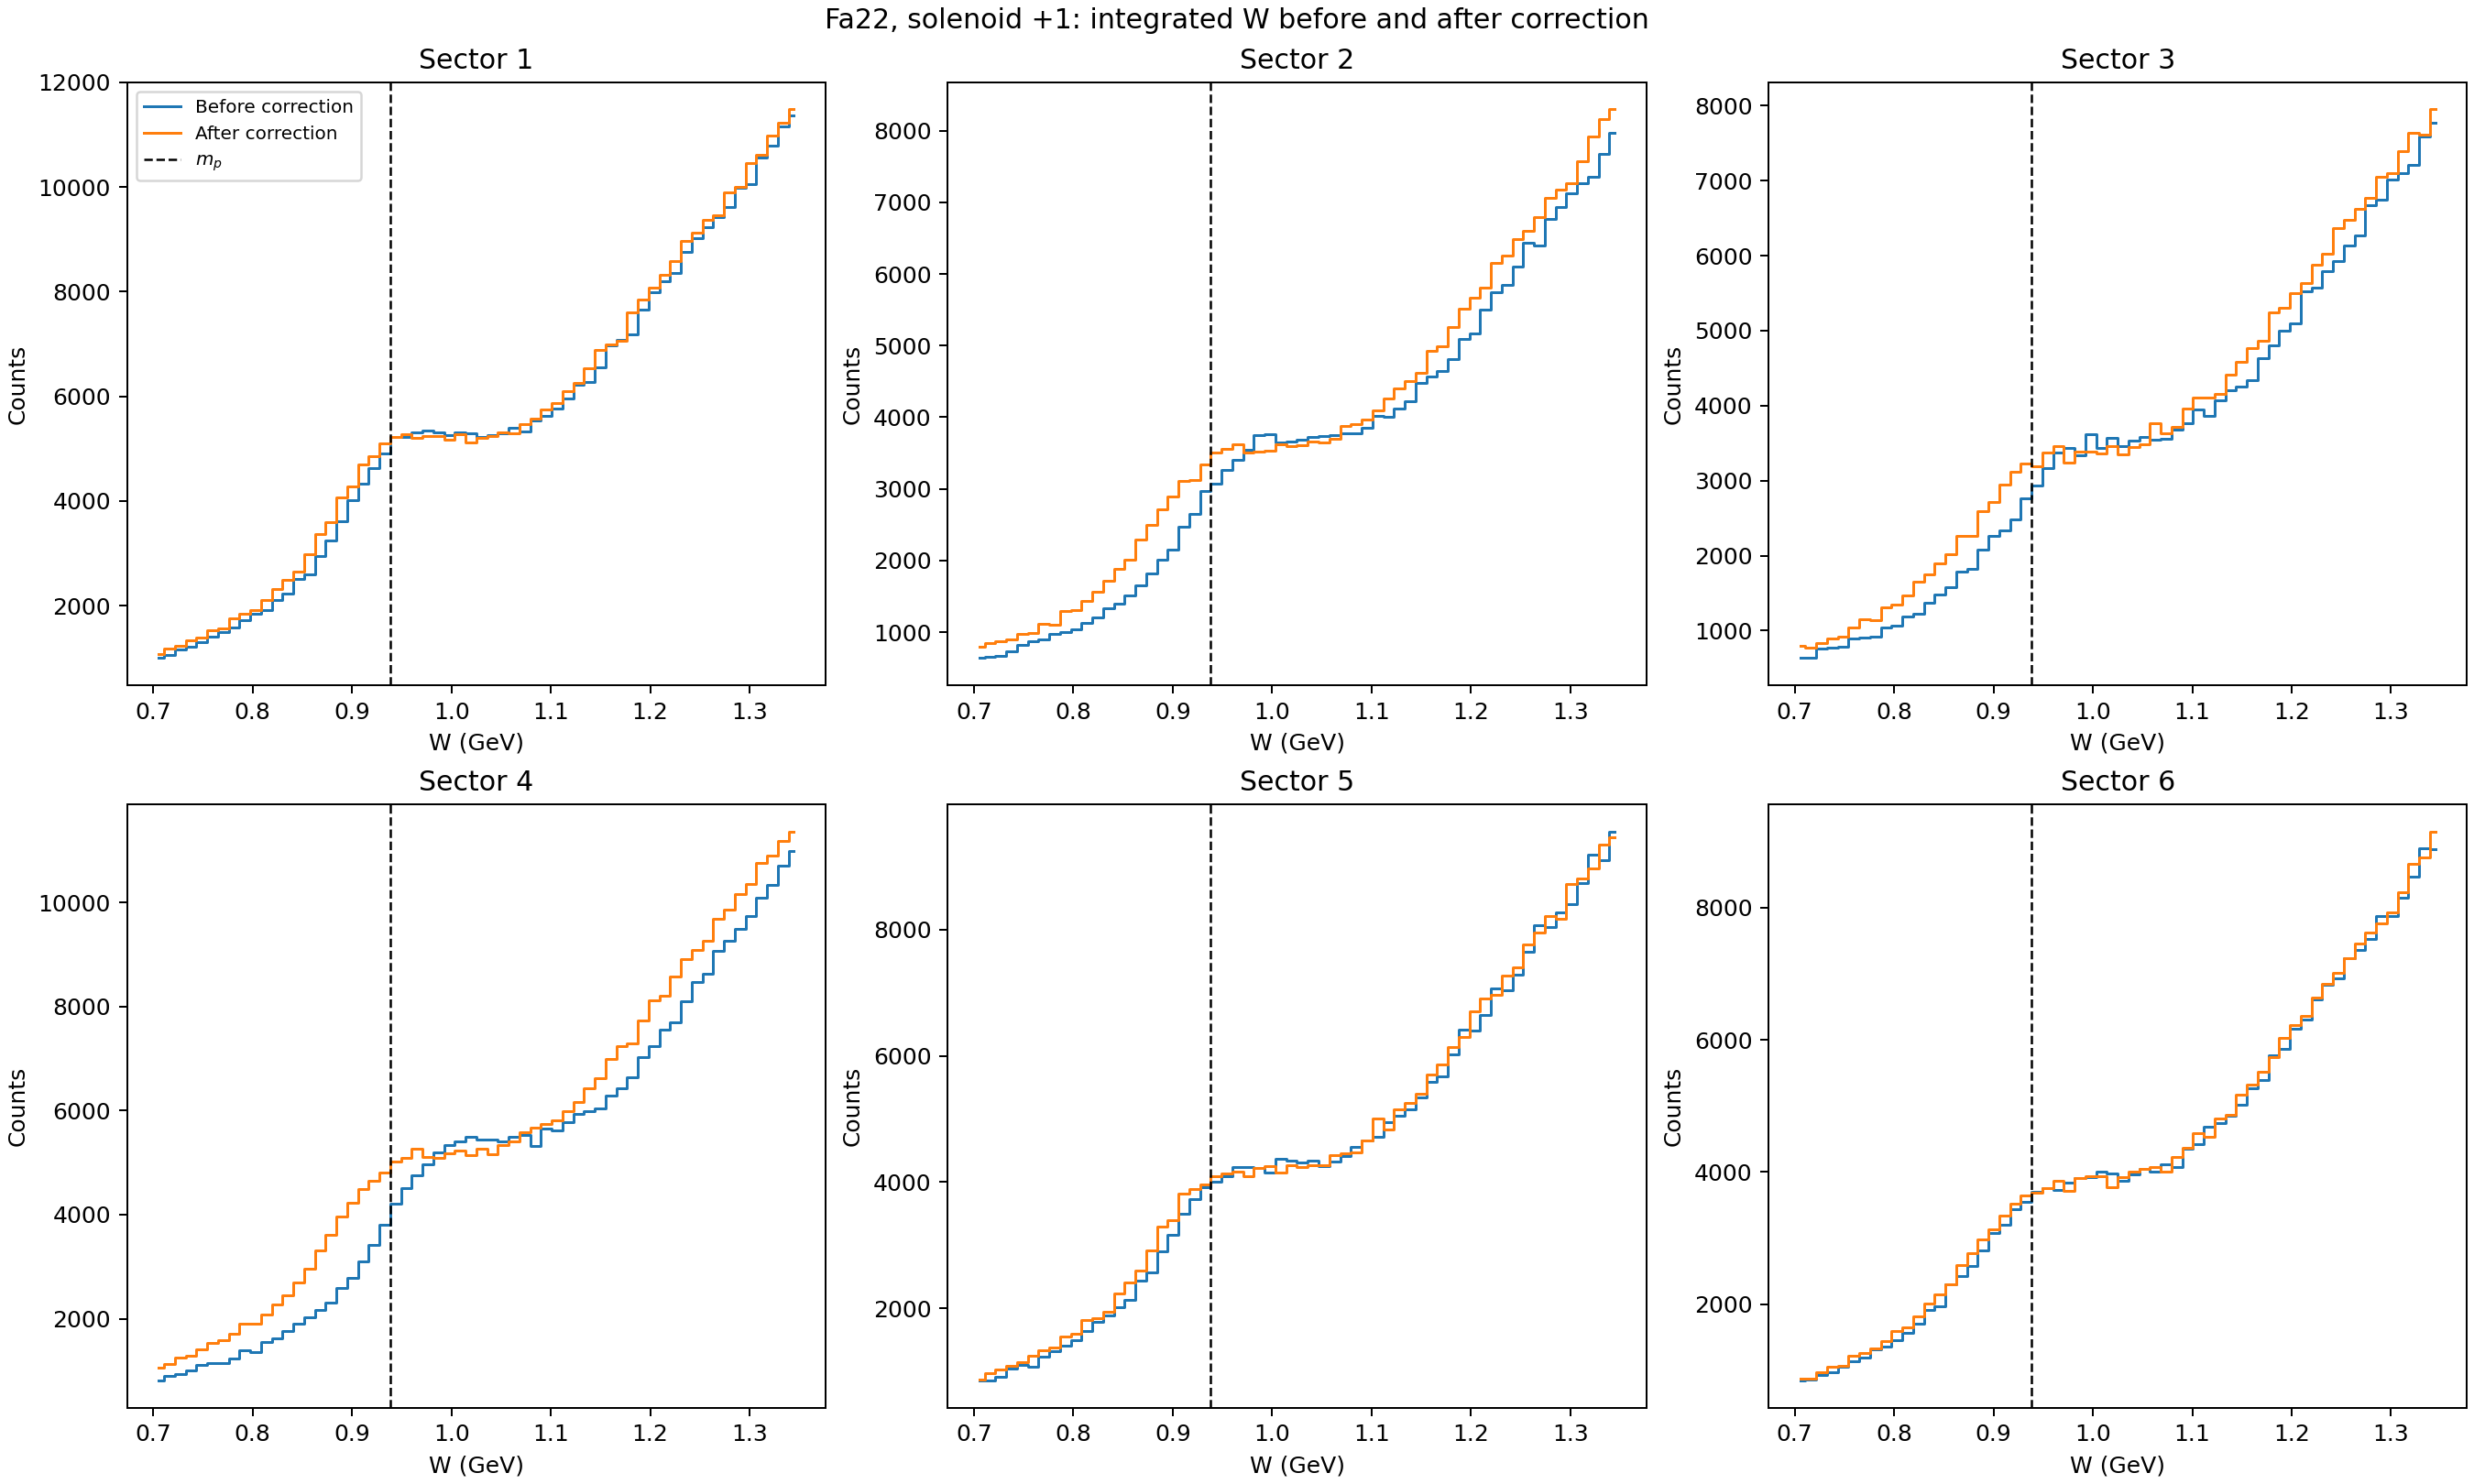
\includegraphics[width=\linewidth]{figures/channel_selection/momentum_corrections/electron/fa22_solenoid_plus_integrated_w_before_after.png}
\end{subfigure}
\caption{Fitted elastic peak position before and after momentum corrections for each of the six sectors of CLAS12 for Fa22 solenoid+1.} % Caption for the whole figure
\label{fig:fa22+1_integrated_before_and_after}
\end{figure}


\begin{figure}[htp]
\internallinenumbers
\begin{subfigure}[t]{0.99\textwidth}
\centering
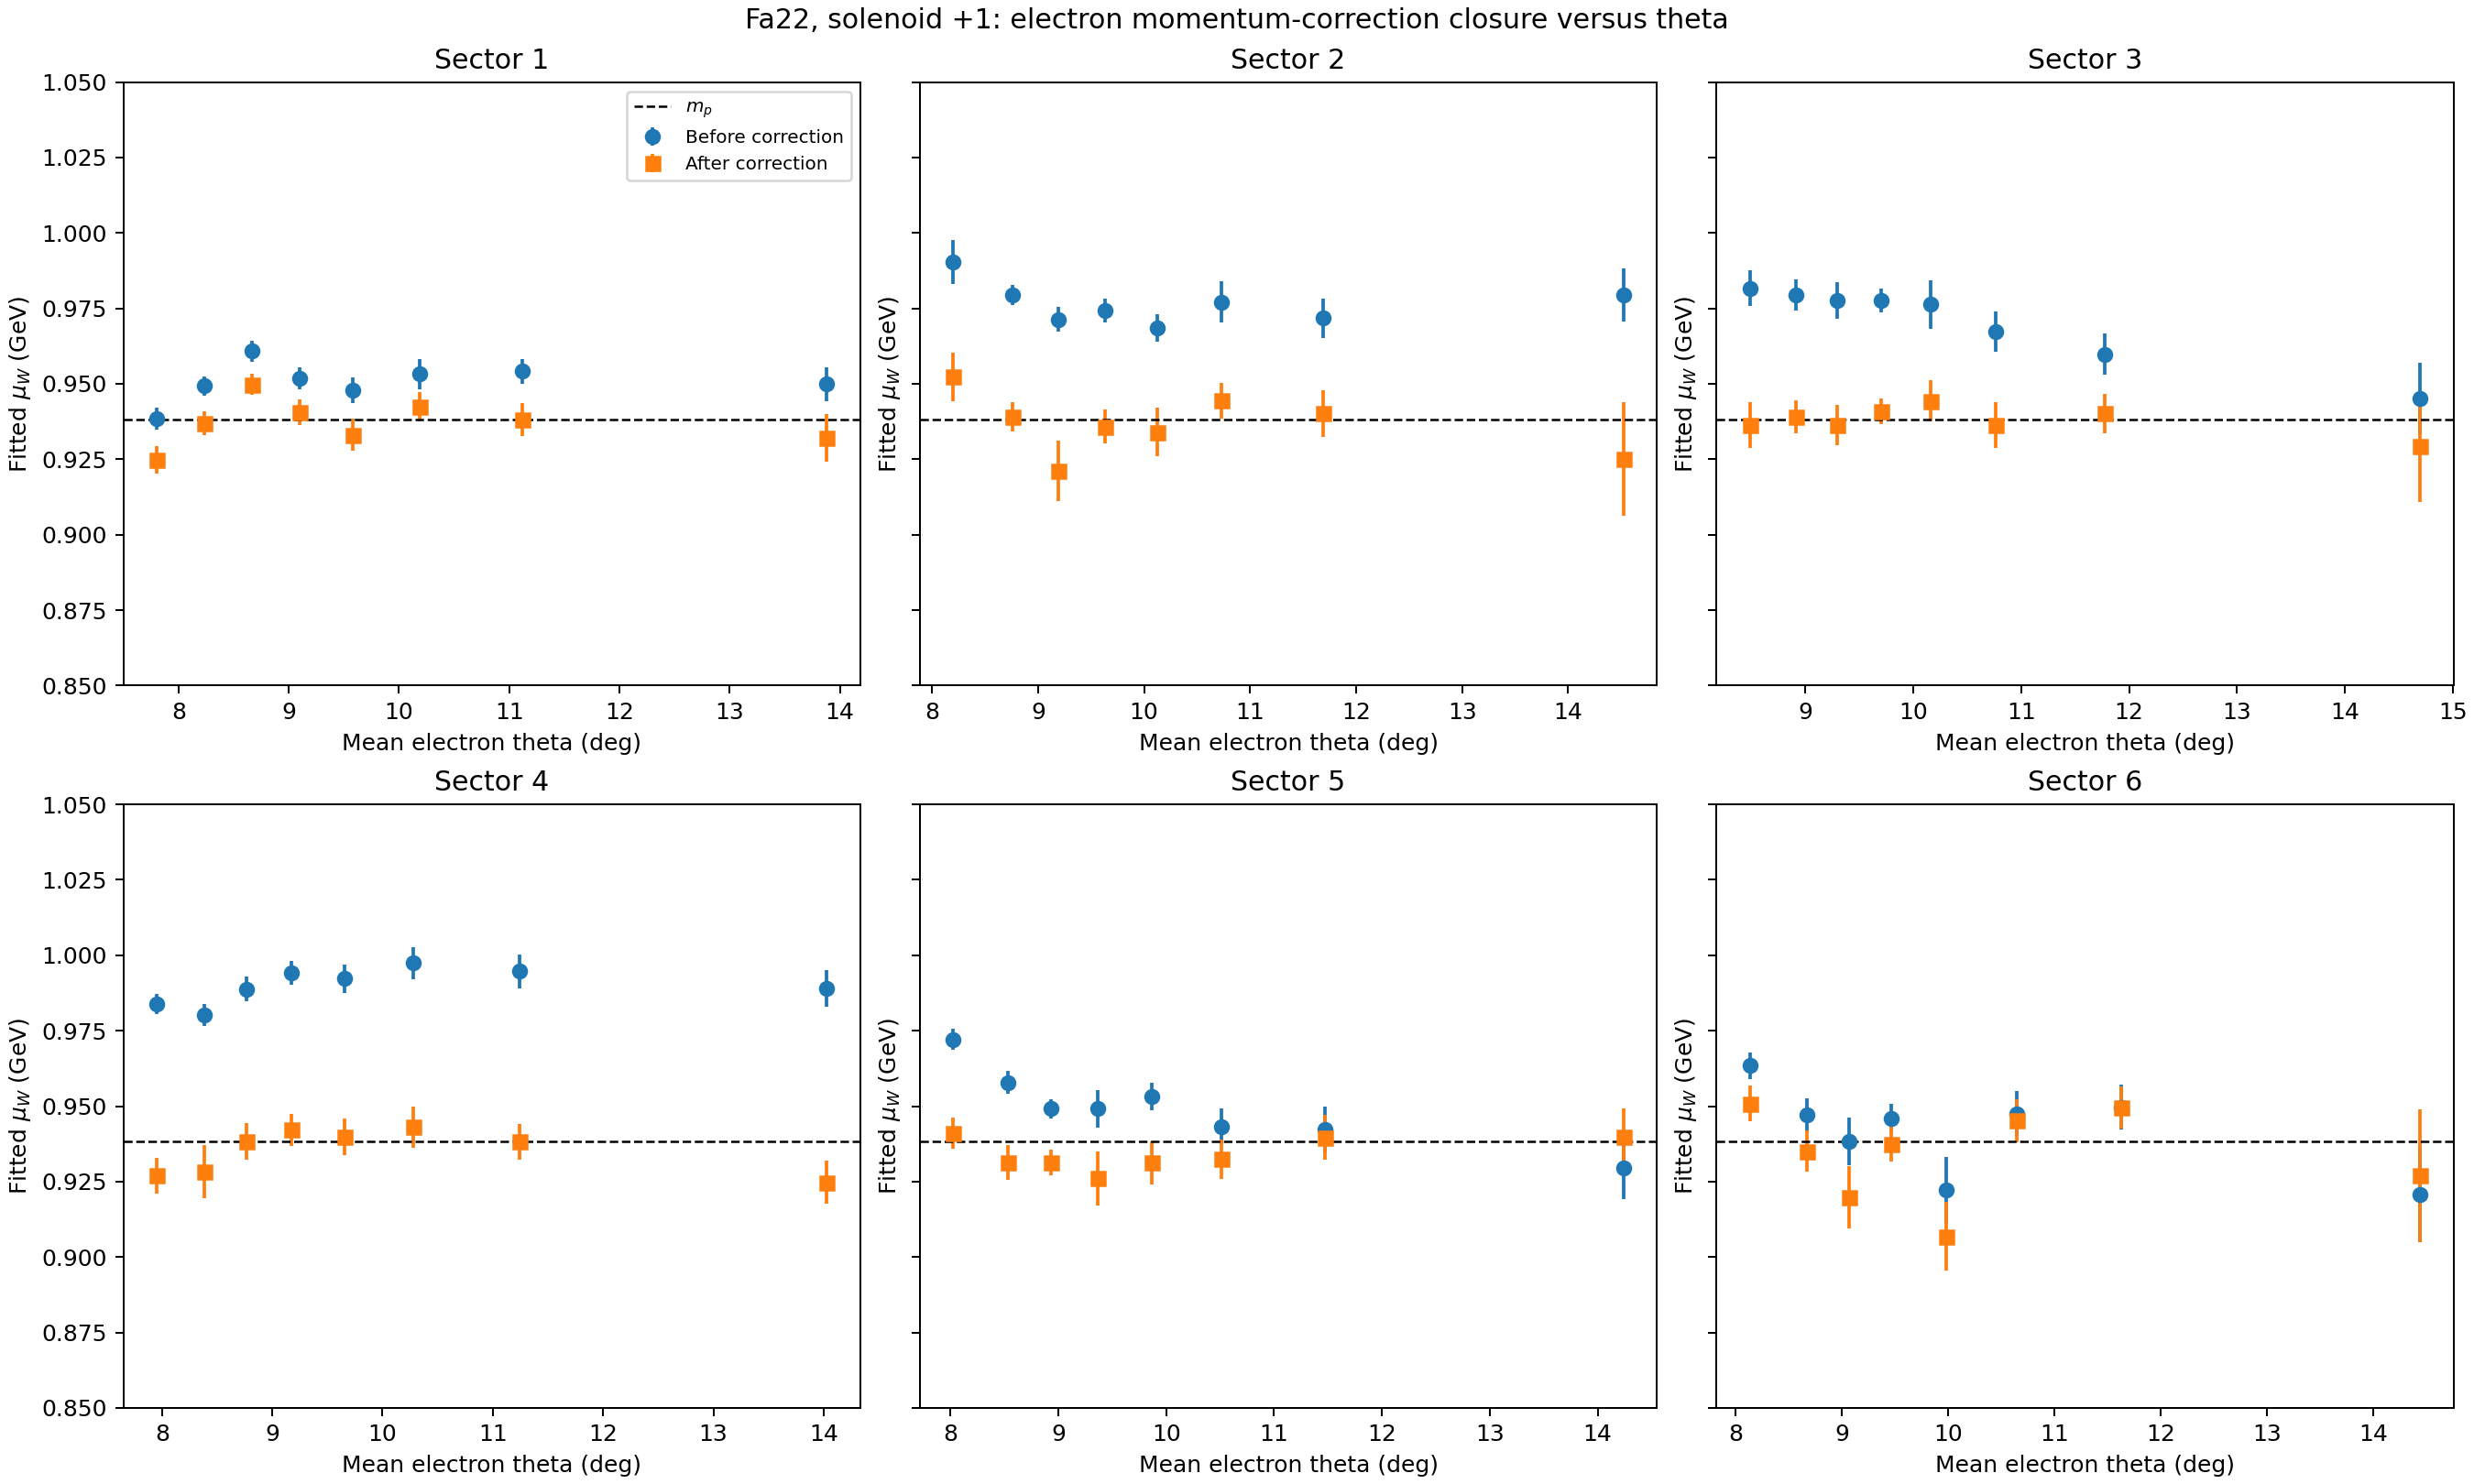
\includegraphics[width=\linewidth]{figures/channel_selection/momentum_corrections/electron/fa22_solenoid_plus_theta_closure.png}
\end{subfigure}
\caption{Fitted elastic peak position before and after momentum corrections for each of the six sectors of CLAS12 for Fa22 solenoid+1 as a function of $e_\theta$} % Caption for the whole figure
\label{fig:fa22_plus_solenoid_theta_before_and_after}
\end{figure}

\begin{figure}[htp]
\internallinenumbers
\begin{subfigure}[t]{0.99\textwidth}
\centering
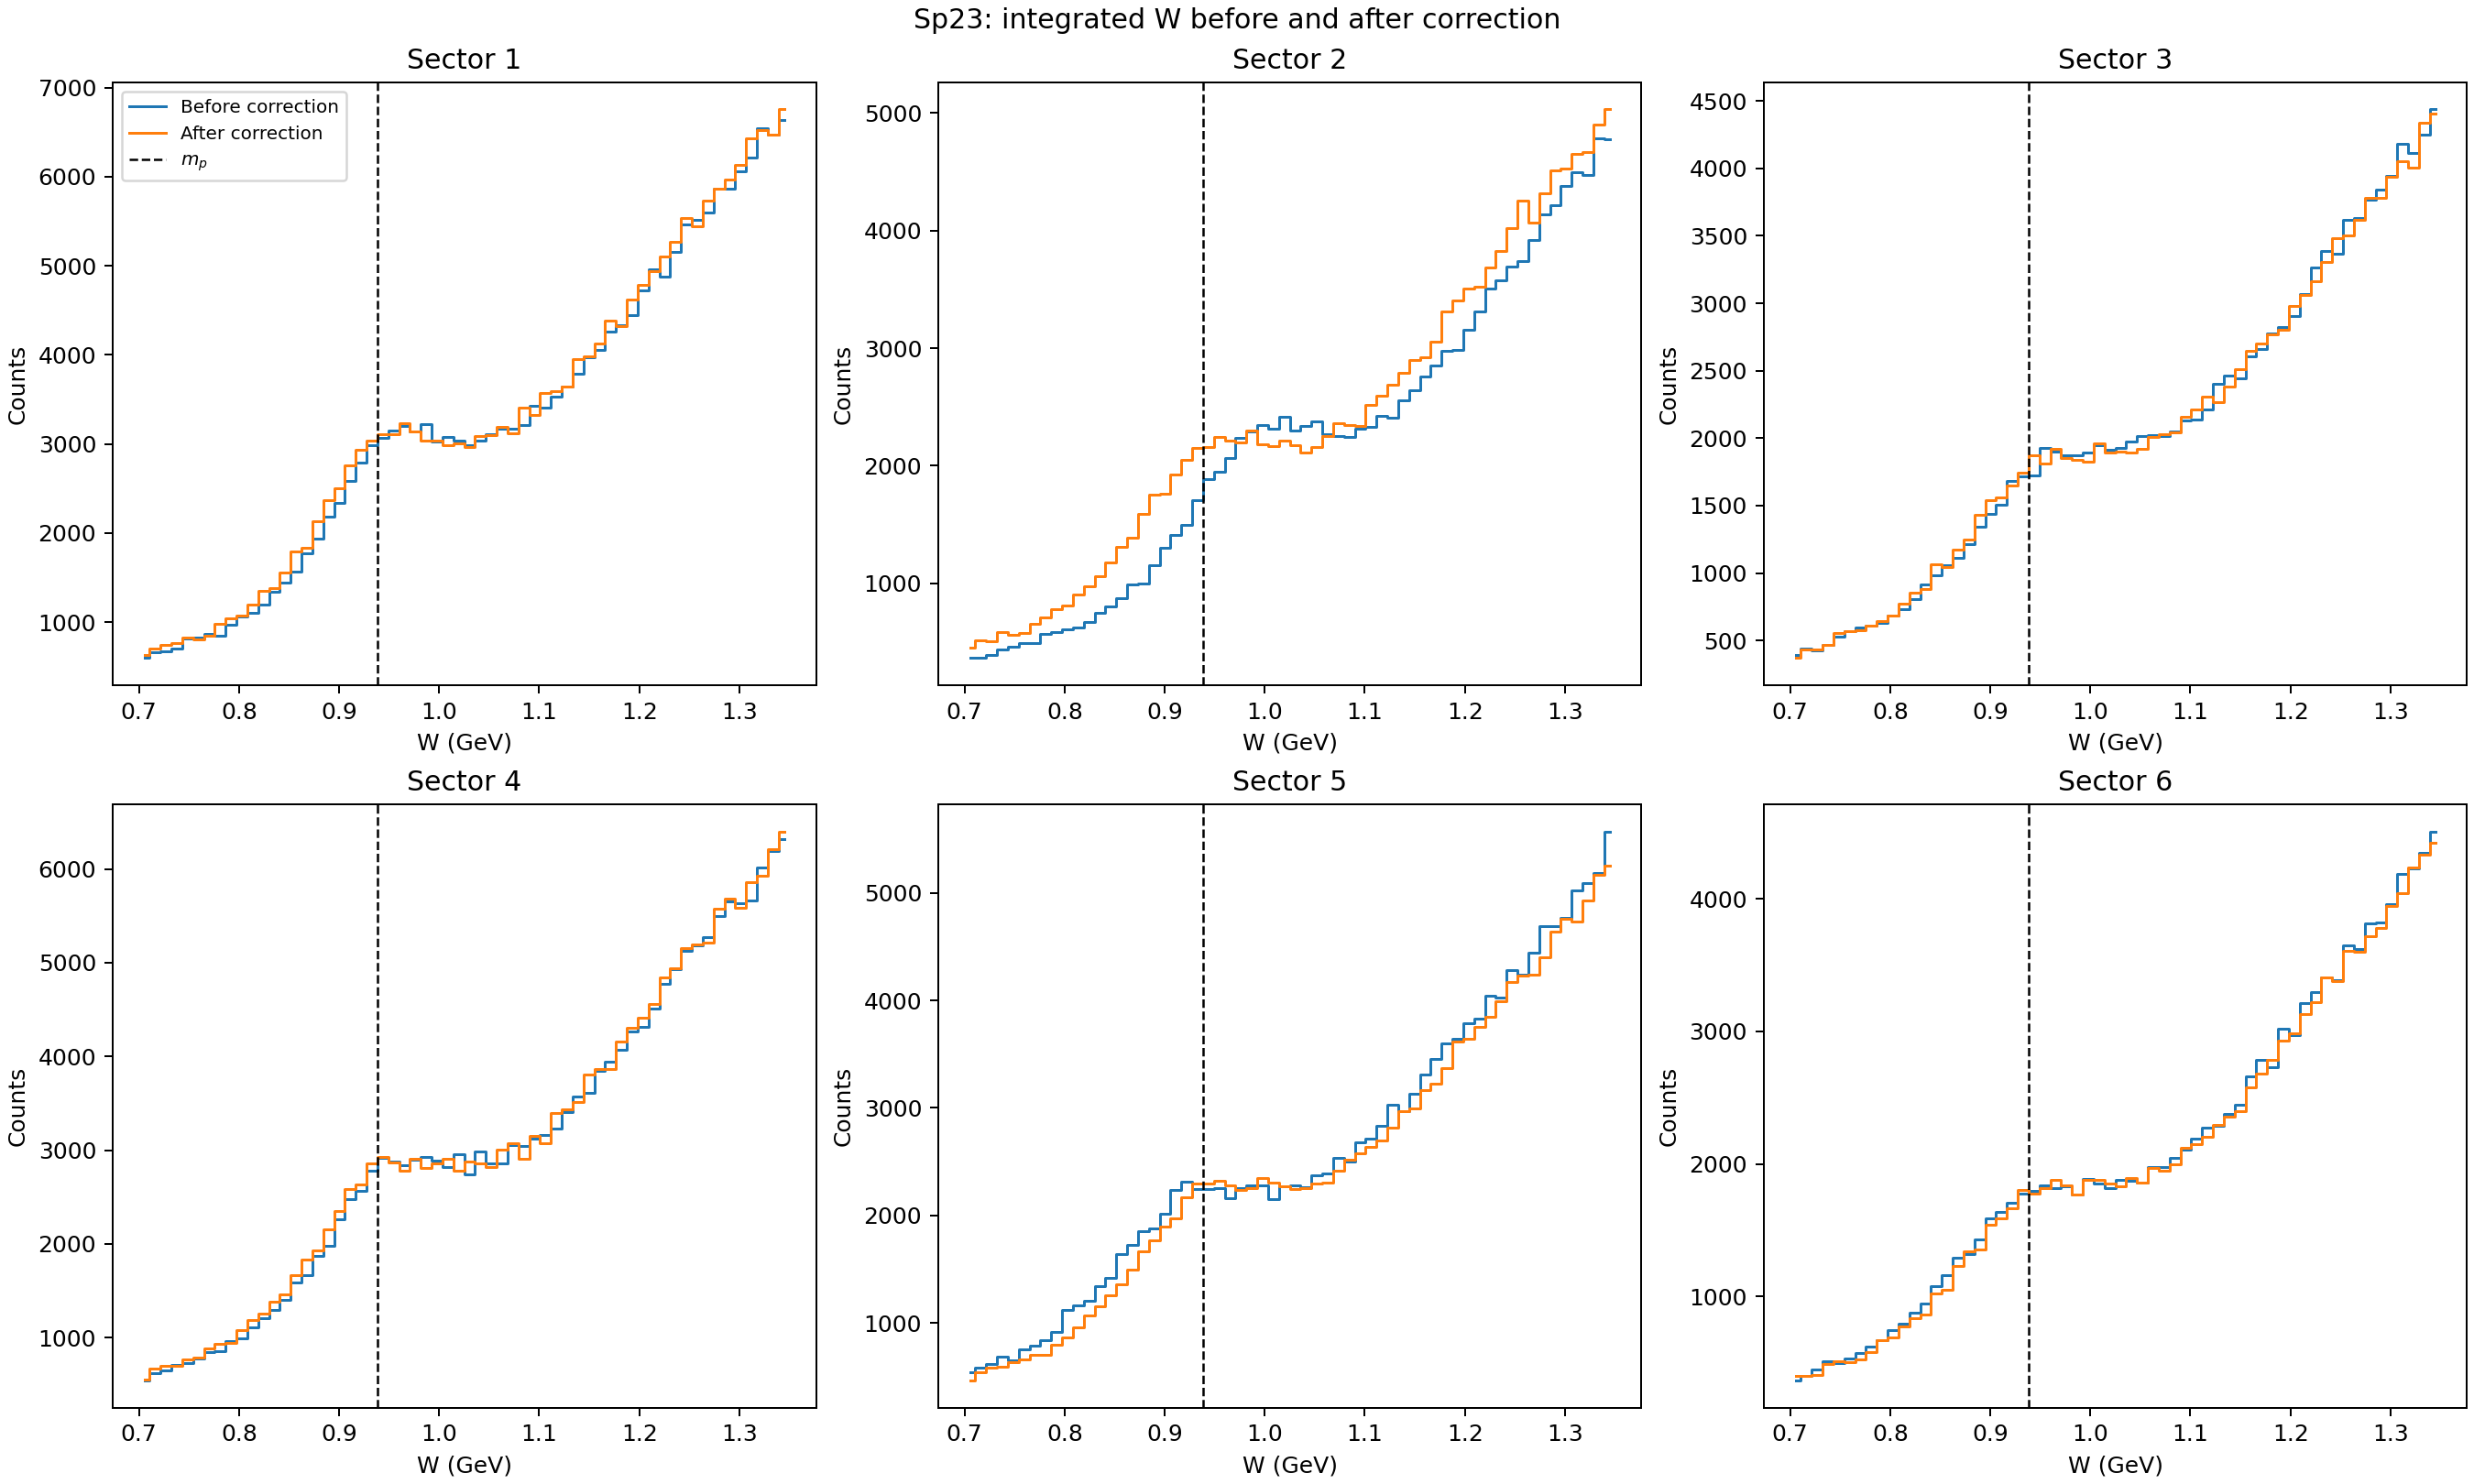
\includegraphics[width=\linewidth]{figures/channel_selection/momentum_corrections/electron/sp23_integrated_w_before_after.png}
\end{subfigure}
\caption{Fitted elastic peak position before and after momentum corrections for each of the six sectors of CLAS12 for Sp23.} % Caption for the whole figure
\label{fig:sp23_integrated_before_and_after}
\end{figure}


\begin{figure}[htp]
\internallinenumbers
\begin{subfigure}[t]{0.99\textwidth}
\centering
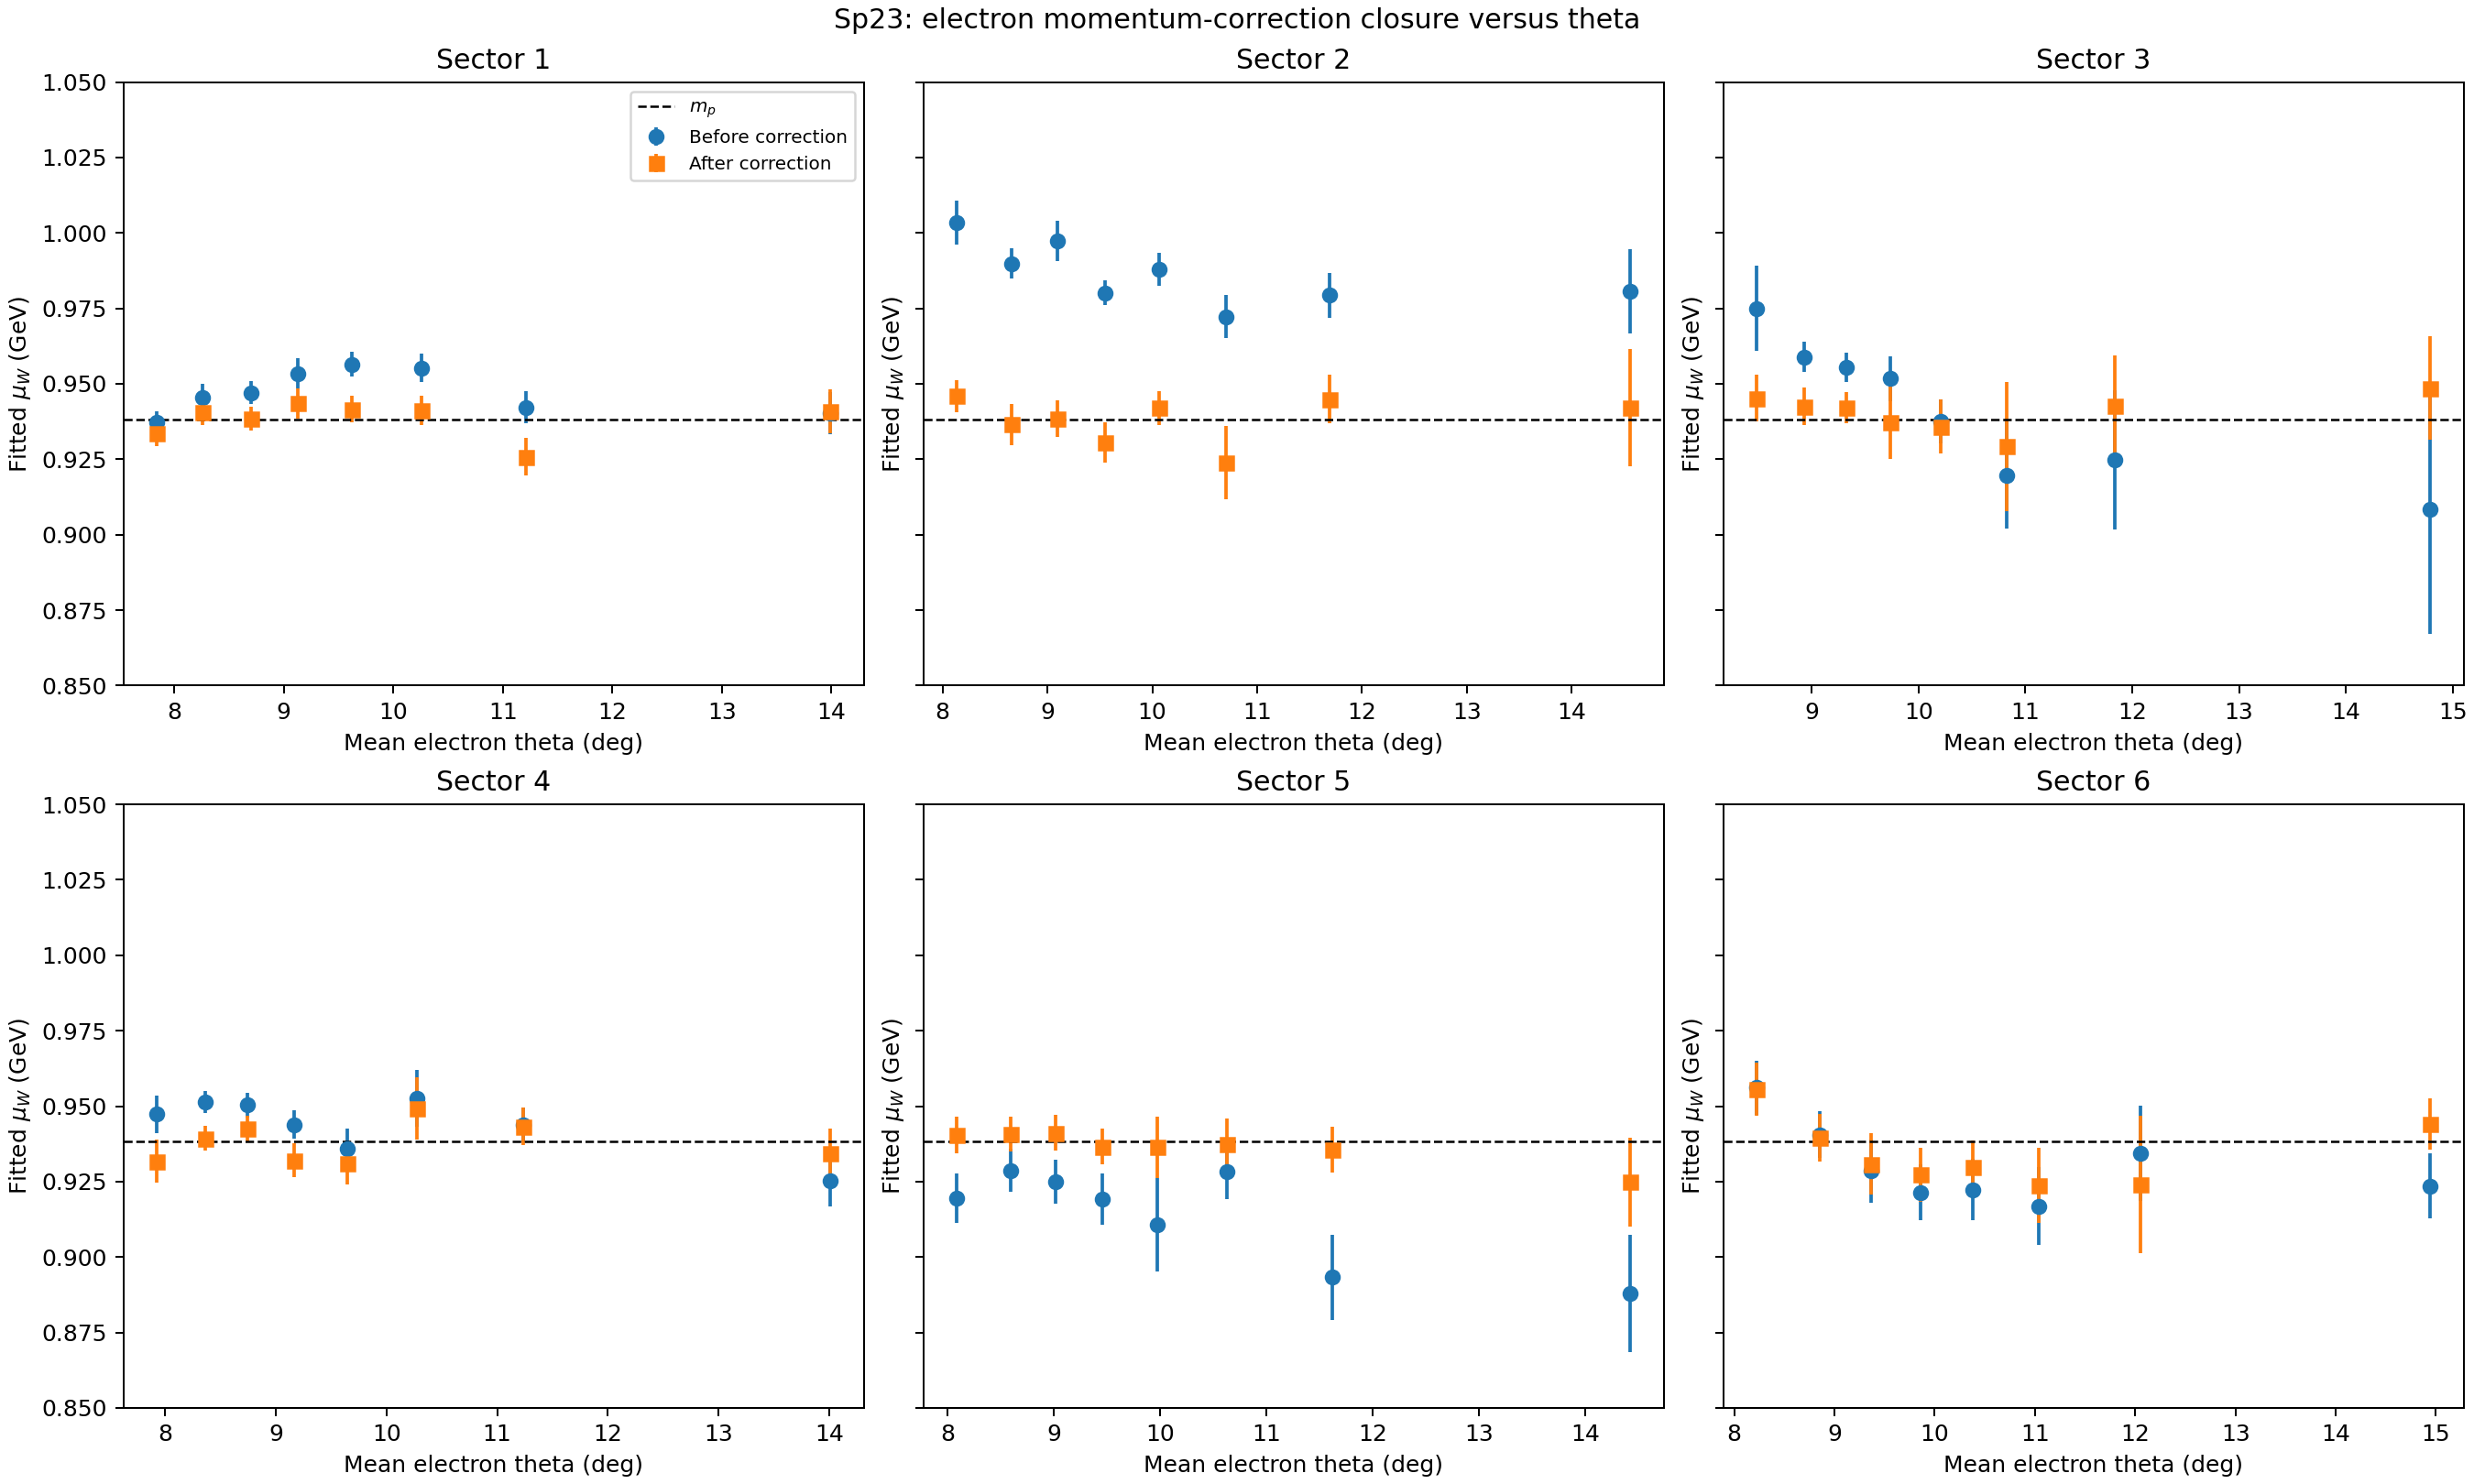
\includegraphics[width=\linewidth]{figures/channel_selection/momentum_corrections/electron/sp23_theta_closure.png}
\end{subfigure}
\caption{Fitted elastic peak position before and after momentum corrections for each of the six sectors of CLAS12 for Sp23 as a function of $e_\theta$} % Caption for the whole figure
\label{fig:sp23_theta_before_and_after}
\end{figure}

\clearpage
Only the electron momentum-correction tables above are transferred to this campaign. Their derivation/control plots are retained from the $\pi^+$ reference analysis, not presented as new ND$_3$ validation plots. The correction is $p_e^{\rm corr}=[1+\delta(\theta_e)]p_e$, with $\theta_e$ clamped to $[8,15]$ degrees and the Fa22 solenoid polarities treated separately. Corrections were also developed for $\pi^+$ in the reference analysis. Those species-specific corrections are not applied to $\pi^-$; corresponding $\pi^-$ corrections can be developed later.

\subsection{Fiducial Cuts}

The preliminary RGC fiducial cuts developed before preliminary releases are currently used in this analysis. They are described in full in the accompanying note \href{https://clas12-docdb.jlab.org/DocDB/0011/001177/002/RGC_Fiducial_Cuts.pdf}{RGC Fiducial Cuts}. In general a minimum ``edge'' variable is enforced in each of the three layers of the drift chamber, cuts on minimum local coordinates $u$ and $v$ in the calorimeter are enforced and several dead PMT/missing strips are removed for improved data and MC matching The effects of these cuts are minimal on the resulting asymmetries.


\subsection{Exclusivity Cuts}\label{sec:exclusivity}
The electron, proton and pion define the deuteron-reference missing mass $M_{X,d}^2=(k+P_d-k'-p_p-p_\pi)^2$ and full spatial missing momentum. Calibration is performed in the original 24 bins, separately for the three RGB periods and RGC Su22, with RGC Fa22+Sp23 pooled for window determination. Each RGC control target receives the same windows as ND$_3$ in its period. Period identities and luminosities remain separate.
A Gaussian spectator-proton peak plus nonnegative linear background defines the mass interval $\mu_M\pm2\sigma_M$. After this cut, a gamma signal plus higher-mode gamma tail describes missing momentum. The selected interval is the signal's central 95.45\% probability interval. A quadratic mass background, a varied tail shape and doubled histogram widths provide diagnostic comparisons. Unresolved Su22 shapes can be transferred from the Fa22+Sp23 reference with documented donor corrections. The signed pion-angle residual is a closure plot and is not an additional cut.
The relaxed sample is recalibrated before the three-bin target refit. All selected events retain their original fine-bin exclusivity windows. Current windows and any reference assistance are retained in the release metadata. The figures below show the new calibration, replacing the earlier sample's fits.
\clearpage
\begin{longtable}{rrrrrl}
\caption{Current exclusivity windows for RGB\_spring2020. Mass-squared boundaries are in GeV$^2$ and missing-momentum boundaries are in GeV.}\\
\toprule Bin & $M^2_{\min}$ & $M^2_{\max}$ & $p_{\min}$ & $p_{\max}$ & Shape source\\\midrule\endhead
1 & 0.7529 & 1.1150 & 0.0244 & 0.2456 & independent\\
2 & 0.7852 & 1.1195 & 0.0263 & 0.2684 & independent\\
3 & 0.7699 & 1.1135 & 0.0275 & 0.2572 & independent\\
4 & 0.7634 & 1.1294 & 0.0292 & 0.2736 & independent\\
5 & 0.7373 & 1.1443 & 0.0307 & 0.2844 & independent\\
6 & 0.7483 & 1.1379 & 0.0290 & 0.2989 & independent\\
7 & 0.7361 & 1.1436 & 0.0254 & 0.2615 & independent\\
8 & 0.7962 & 1.1357 & 0.0291 & 0.2880 & independent\\
9 & 0.7930 & 1.1376 & 0.0289 & 0.2695 & independent\\
10 & 0.7989 & 1.1137 & 0.0265 & 0.2556 & independent\\
11 & 0.7844 & 1.1151 & 0.0278 & 0.2439 & independent\\
12 & 0.8106 & 1.1023 & 0.0278 & 0.2385 & independent\\
13 & 0.7283 & 1.1687 & 0.0268 & 0.2654 & independent\\
14 & 0.7674 & 1.1619 & 0.0289 & 0.2938 & independent\\
15 & 0.8046 & 1.1247 & 0.0287 & 0.2780 & independent\\
16 & 0.8071 & 1.1201 & 0.0279 & 0.2841 & independent\\
17 & 0.7979 & 1.1257 & 0.0270 & 0.2552 & independent\\
18 & 0.7828 & 1.1403 & 0.0290 & 0.2671 & independent\\
19 & 0.7219 & 1.1967 & 0.0265 & 0.2743 & independent\\
20 & 0.7502 & 1.2018 & 0.0290 & 0.2939 & independent\\
21 & 0.7740 & 1.1569 & 0.0291 & 0.2925 & independent\\
22 & 0.7836 & 1.1415 & 0.0286 & 0.2918 & independent\\
23 & 0.7795 & 1.1512 & 0.0286 & 0.2805 & independent\\
24 & 0.7693 & 1.1718 & 0.0296 & 0.2946 & independent\\
\bottomrule\end{longtable}
\clearpage
\begin{longtable}{rrrrrl}
\caption{Current exclusivity windows for RGC\_fall2022\_spring2023. Mass-squared boundaries are in GeV$^2$ and missing-momentum boundaries are in GeV.}\\
\toprule Bin & $M^2_{\min}$ & $M^2_{\max}$ & $p_{\min}$ & $p_{\max}$ & Shape source\\\midrule\endhead
1 & 0.7138 & 1.1728 & 0.0408 & 0.4729 & independent\\
2 & 0.7627 & 1.1786 & 0.0358 & 0.4236 & independent\\
3 & 0.8015 & 1.1453 & 0.0394 & 0.3993 & independent\\
4 & 0.7833 & 1.1448 & 0.0390 & 0.4039 & independent\\
5 & 0.7475 & 1.1051 & 0.0370 & 0.3952 & independent\\
6 & 0.7985 & 1.1388 & 0.0381 & 0.4168 & independent\\
7 & 0.7132 & 1.1781 & 0.0364 & 0.3946 & independent\\
8 & 0.7810 & 1.1752 & 0.0419 & 0.4091 & independent\\
9 & 0.8056 & 1.1527 & 0.0376 & 0.3918 & independent\\
10 & 0.7864 & 1.1557 & 0.0392 & 0.3803 & independent\\
11 & 0.7670 & 1.1716 & 0.0395 & 0.3962 & independent\\
12 & 0.8216 & 1.1473 & 0.0398 & 0.3811 & independent\\
13 & 0.7215 & 1.1895 & 0.0359 & 0.3629 & independent\\
14 & 0.7656 & 1.2013 & 0.0407 & 0.3987 & independent\\
15 & 0.8146 & 1.1670 & 0.0428 & 0.4275 & independent\\
16 & 0.7977 & 1.1804 & 0.0434 & 0.4530 & independent\\
17 & 0.8416 & 1.1264 & 0.0406 & 0.4275 & independent\\
18 & 0.8120 & 1.1523 & 0.0423 & 0.4464 & independent\\
19 & 0.7473 & 1.1870 & 0.0333 & 0.3829 & independent\\
20 & 0.7722 & 1.2074 & 0.0378 & 0.3817 & independent\\
21 & 0.7922 & 1.1795 & 0.0400 & 0.3711 & independent\\
22 & 0.7972 & 1.1651 & 0.0400 & 0.3948 & independent\\
23 & 0.8186 & 1.1490 & 0.0409 & 0.3987 & independent\\
24 & 0.7972 & 1.1477 & 0.0418 & 0.4259 & independent\\
\bottomrule\end{longtable}
\clearpage
\begin{longtable}{rrrrrl}
\caption{Current exclusivity windows for RGB\_fall2019. Mass-squared boundaries are in GeV$^2$ and missing-momentum boundaries are in GeV.}\\
\toprule Bin & $M^2_{\min}$ & $M^2_{\max}$ & $p_{\min}$ & $p_{\max}$ & Shape source\\\midrule\endhead
1 & 0.7469 & 1.1264 & 0.0237 & 0.2422 & independent\\
2 & 0.7747 & 1.1224 & 0.0252 & 0.2535 & independent\\
3 & 0.7481 & 1.1222 & 0.0271 & 0.2547 & independent\\
4 & 0.7249 & 1.1232 & 0.0281 & 0.2679 & independent\\
5 & 0.7036 & 1.1204 & 0.0293 & 0.2670 & independent\\
6 & 0.7946 & 1.0648 & 0.0255 & 0.2917 & independent\\
7 & 0.7285 & 1.1327 & 0.0240 & 0.2471 & independent\\
8 & 0.7609 & 1.1185 & 0.0257 & 0.2574 & independent\\
9 & 0.7471 & 1.1110 & 0.0268 & 0.2606 & independent\\
10 & 0.7663 & 1.0688 & 0.0252 & 0.2463 & independent\\
11 & 0.7257 & 1.0897 & 0.0278 & 0.2479 & independent\\
12 & 0.7484 & 1.0631 & 0.0278 & 0.2407 & independent\\
13 & 0.7041 & 1.1597 & 0.0253 & 0.2564 & independent\\
14 & 0.7476 & 1.1437 & 0.0269 & 0.2804 & independent\\
15 & 0.7585 & 1.1296 & 0.0289 & 0.2846 & independent\\
16 & 0.7530 & 1.0851 & 0.0270 & 0.2511 & independent\\
17 & 0.7636 & 1.0991 & 0.0270 & 0.2550 & independent\\
18 & 0.7289 & 1.0987 & 0.0282 & 0.2393 & independent\\
19 & 0.7016 & 1.1839 & 0.0275 & 0.2545 & independent\\
20 & 0.6963 & 1.2490 & 0.0296 & 0.3310 & independent\\
21 & 0.7678 & 1.1305 & 0.0283 & 0.2789 & independent\\
22 & 0.7270 & 1.1157 & 0.0295 & 0.2688 & independent\\
23 & 0.7523 & 1.1071 & 0.0253 & 0.2738 & independent\\
24 & 0.7109 & 1.1201 & 0.0275 & 0.2834 & independent\\
\bottomrule\end{longtable}
\clearpage
\begin{longtable}{rrrrrl}
\caption{Current exclusivity windows for RGB\_spring2019. Mass-squared boundaries are in GeV$^2$ and missing-momentum boundaries are in GeV.}\\
\toprule Bin & $M^2_{\min}$ & $M^2_{\max}$ & $p_{\min}$ & $p_{\max}$ & Shape source\\\midrule\endhead
1 & 0.7208 & 1.0844 & 0.0226 & 0.2266 & independent\\
2 & 0.7460 & 1.0883 & 0.0241 & 0.2408 & independent\\
3 & 0.7306 & 1.0828 & 0.0252 & 0.2452 & independent\\
4 & 0.7264 & 1.0954 & 0.0250 & 0.2568 & independent\\
5 & 0.7206 & 1.0839 & 0.0258 & 0.2660 & independent\\
6 & 0.7155 & 1.0825 & 0.0275 & 0.2577 & independent\\
7 & 0.7159 & 1.1046 & 0.0236 & 0.2447 & independent\\
8 & 0.7649 & 1.0888 & 0.0252 & 0.2522 & independent\\
9 & 0.7514 & 1.0947 & 0.0254 & 0.2469 & independent\\
10 & 0.7804 & 1.0709 & 0.0247 & 0.2305 & independent\\
11 & 0.7580 & 1.0749 & 0.0254 & 0.2404 & independent\\
12 & 0.7566 & 1.0836 & 0.0263 & 0.2402 & independent\\
13 & 0.6976 & 1.1448 & 0.0256 & 0.2503 & independent\\
14 & 0.7392 & 1.1224 & 0.0265 & 0.2734 & independent\\
15 & 0.7690 & 1.0822 & 0.0252 & 0.2614 & independent\\
16 & 0.7658 & 1.0848 & 0.0253 & 0.2470 & independent\\
17 & 0.7855 & 1.0603 & 0.0244 & 0.2274 & independent\\
18 & 0.7479 & 1.0902 & 0.0250 & 0.2369 & independent\\
19 & 0.6872 & 1.1822 & 0.0253 & 0.2626 & independent\\
20 & 0.7116 & 1.1676 & 0.0271 & 0.2806 & independent\\
21 & 0.7156 & 1.1292 & 0.0272 & 0.2850 & independent\\
22 & 0.7484 & 1.0824 & 0.0255 & 0.2695 & independent\\
23 & 0.7100 & 1.1246 & 0.0280 & 0.2772 & independent\\
24 & 0.7391 & 1.0948 & 0.0256 & 0.2522 & independent\\
\bottomrule\end{longtable}
\clearpage
\begin{longtable}{rrrrrl}
\caption{Current exclusivity windows for RGC\_summer2022. Mass-squared boundaries are in GeV$^2$ and missing-momentum boundaries are in GeV.}\\
\toprule Bin & $M^2_{\min}$ & $M^2_{\max}$ & $p_{\min}$ & $p_{\max}$ & Shape source\\\midrule\endhead
1 & 0.7179 & 1.1481 & 0.0384 & 0.4861 & independent\\
2 & 0.7799 & 1.0820 & 0.0319 & 0.3513 & independent\\
3 & 0.7768 & 1.0942 & 0.0338 & 0.3430 & independent\\
4 & 0.8709 & 0.9944 & 0.0351 & 0.2998 & independent\\
5 & 0.7247 & 1.0597 & 0.0376 & 0.3639 & reference-assisted\\
6 & 0.7752 & 1.0939 & 0.0361 & 0.3855 & reference-assisted\\
7 & 0.6944 & 1.1840 & 0.0372 & 0.4334 & independent\\
8 & 0.7725 & 1.1406 & 0.0395 & 0.4215 & independent\\
9 & 0.7959 & 1.1219 & 0.0385 & 0.4544 & independent\\
10 & 0.7014 & 1.1723 & 0.0375 & 0.3928 & independent\\
11 & 0.8130 & 1.0392 & 0.0310 & 0.2811 & independent\\
12 & 0.7978 & 1.1029 & 0.0360 & 0.3829 & reference-assisted\\
13 & 0.6840 & 1.1806 & 0.0343 & 0.3783 & independent\\
14 & 0.7437 & 1.1673 & 0.0383 & 0.4035 & independent\\
15 & 0.7501 & 1.0847 & 0.0408 & 0.4599 & independent\\
16 & 0.8007 & 1.0835 & 0.0395 & 0.4247 & independent\\
17 & 0.7518 & 1.1737 & 0.0443 & 0.5015 & independent\\
18 & 0.8382 & 0.9178 & 0.0320 & 0.2380 & independent\\
19 & 0.6775 & 1.1949 & 0.0322 & 0.3629 & independent\\
20 & 0.6996 & 1.2301 & 0.0381 & 0.3963 & independent\\
21 & 0.7574 & 1.1485 & 0.0399 & 0.3705 & independent\\
22 & 0.7746 & 1.1140 & 0.0418 & 0.4060 & independent\\
23 & 0.7537 & 1.1025 & 0.0408 & 0.4184 & independent\\
24 & 0.7123 & 1.2052 & 0.0465 & 0.4610 & independent\\
\bottomrule\end{longtable}

\begin{figure}[p]\centering
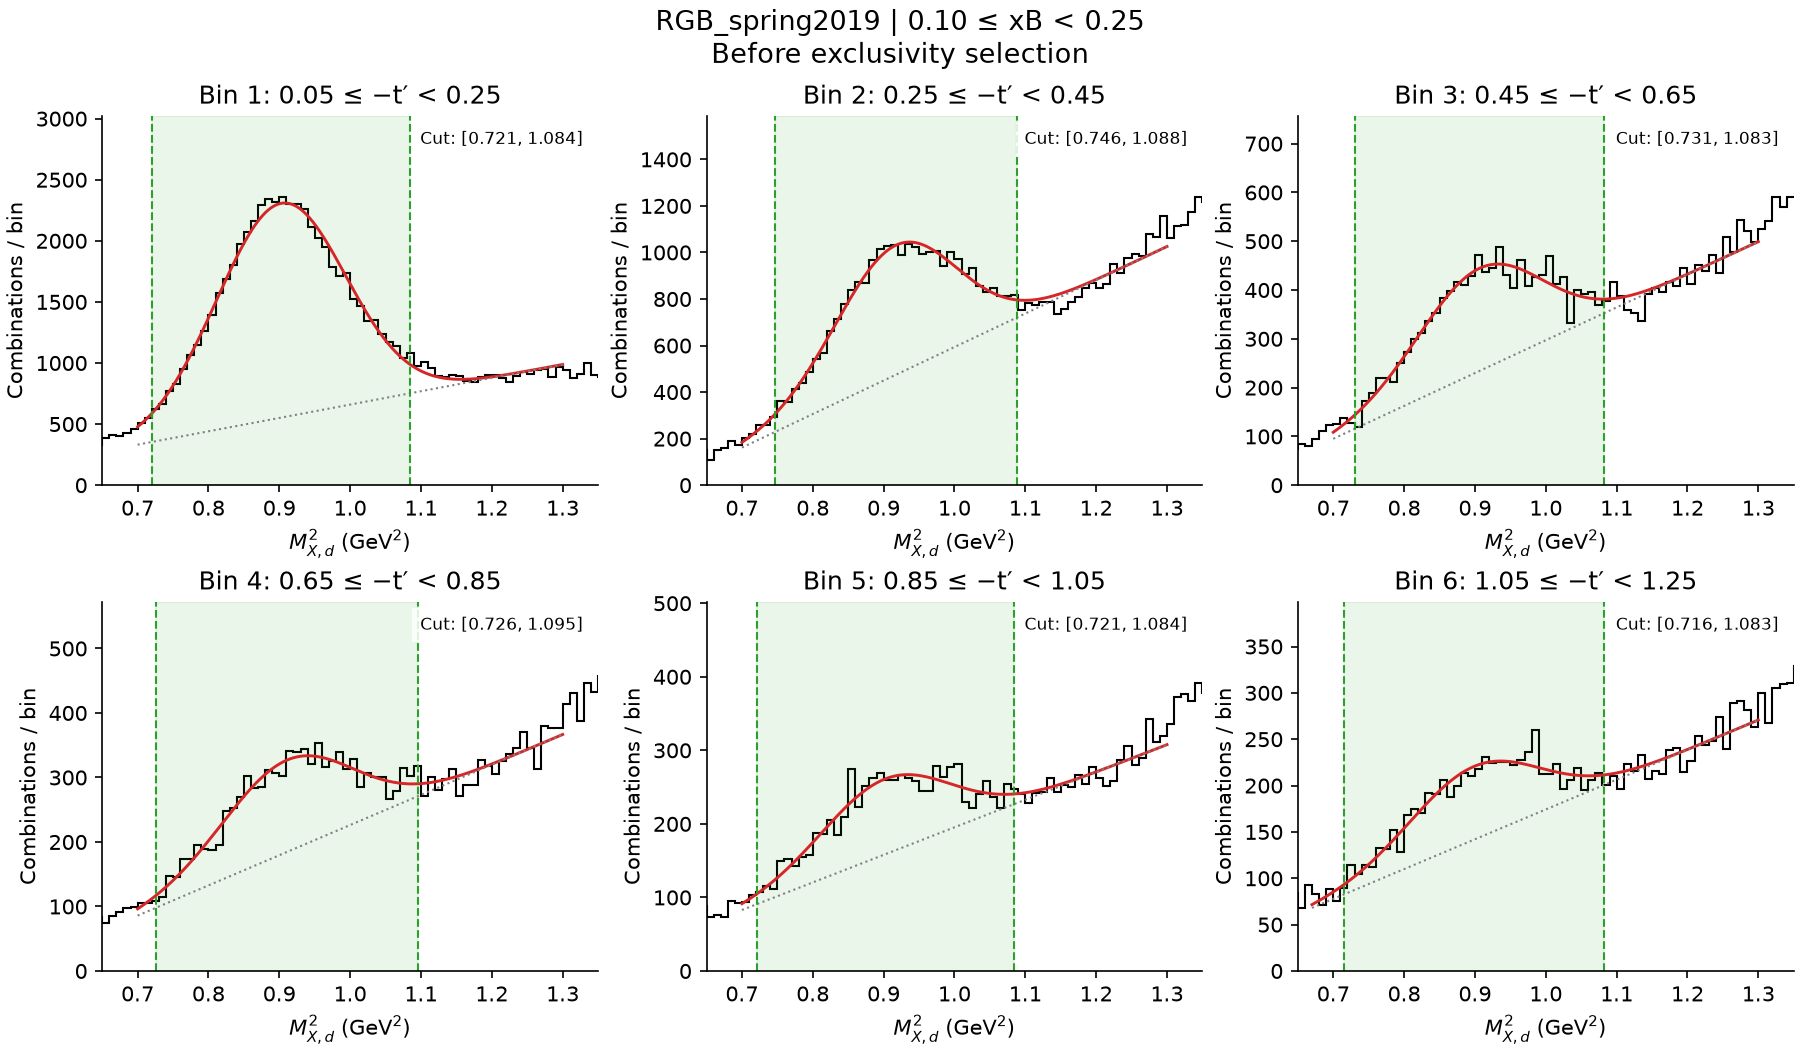
\includegraphics[width=\linewidth]{figures/channel_selection/exclusivity/rgb_sp19_mass_xb1.png}
\caption{RGB\_spring2019: deuteron-reference missing-mass-squared fits in $x_B$ interval 1. The panels retain the six fine selection bins.}\label{fig:new_excl_rgb_sp19_mass1}
\end{figure}
\clearpage
\begin{figure}[p]\centering
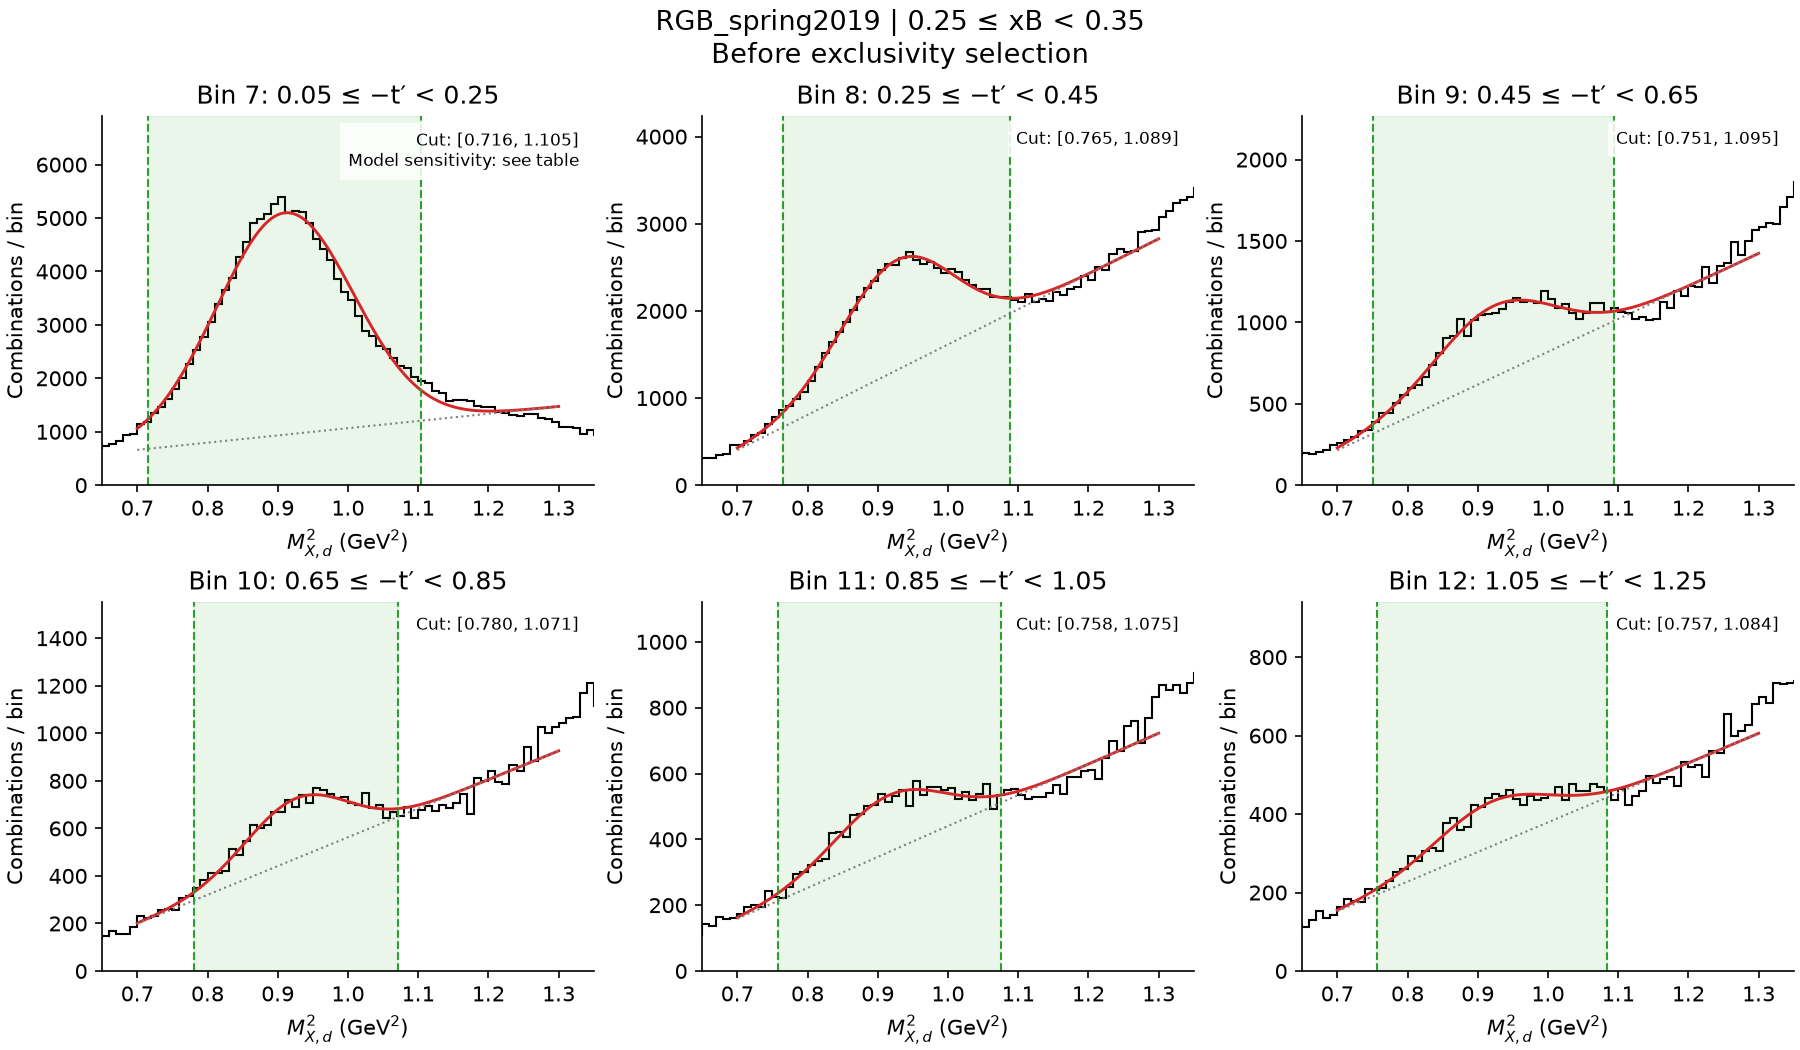
\includegraphics[width=\linewidth]{figures/channel_selection/exclusivity/rgb_sp19_mass_xb2.png}
\caption{RGB\_spring2019: deuteron-reference missing-mass-squared fits in $x_B$ interval 2. The panels retain the six fine selection bins.}\label{fig:new_excl_rgb_sp19_mass2}
\end{figure}
\clearpage
\begin{figure}[p]\centering
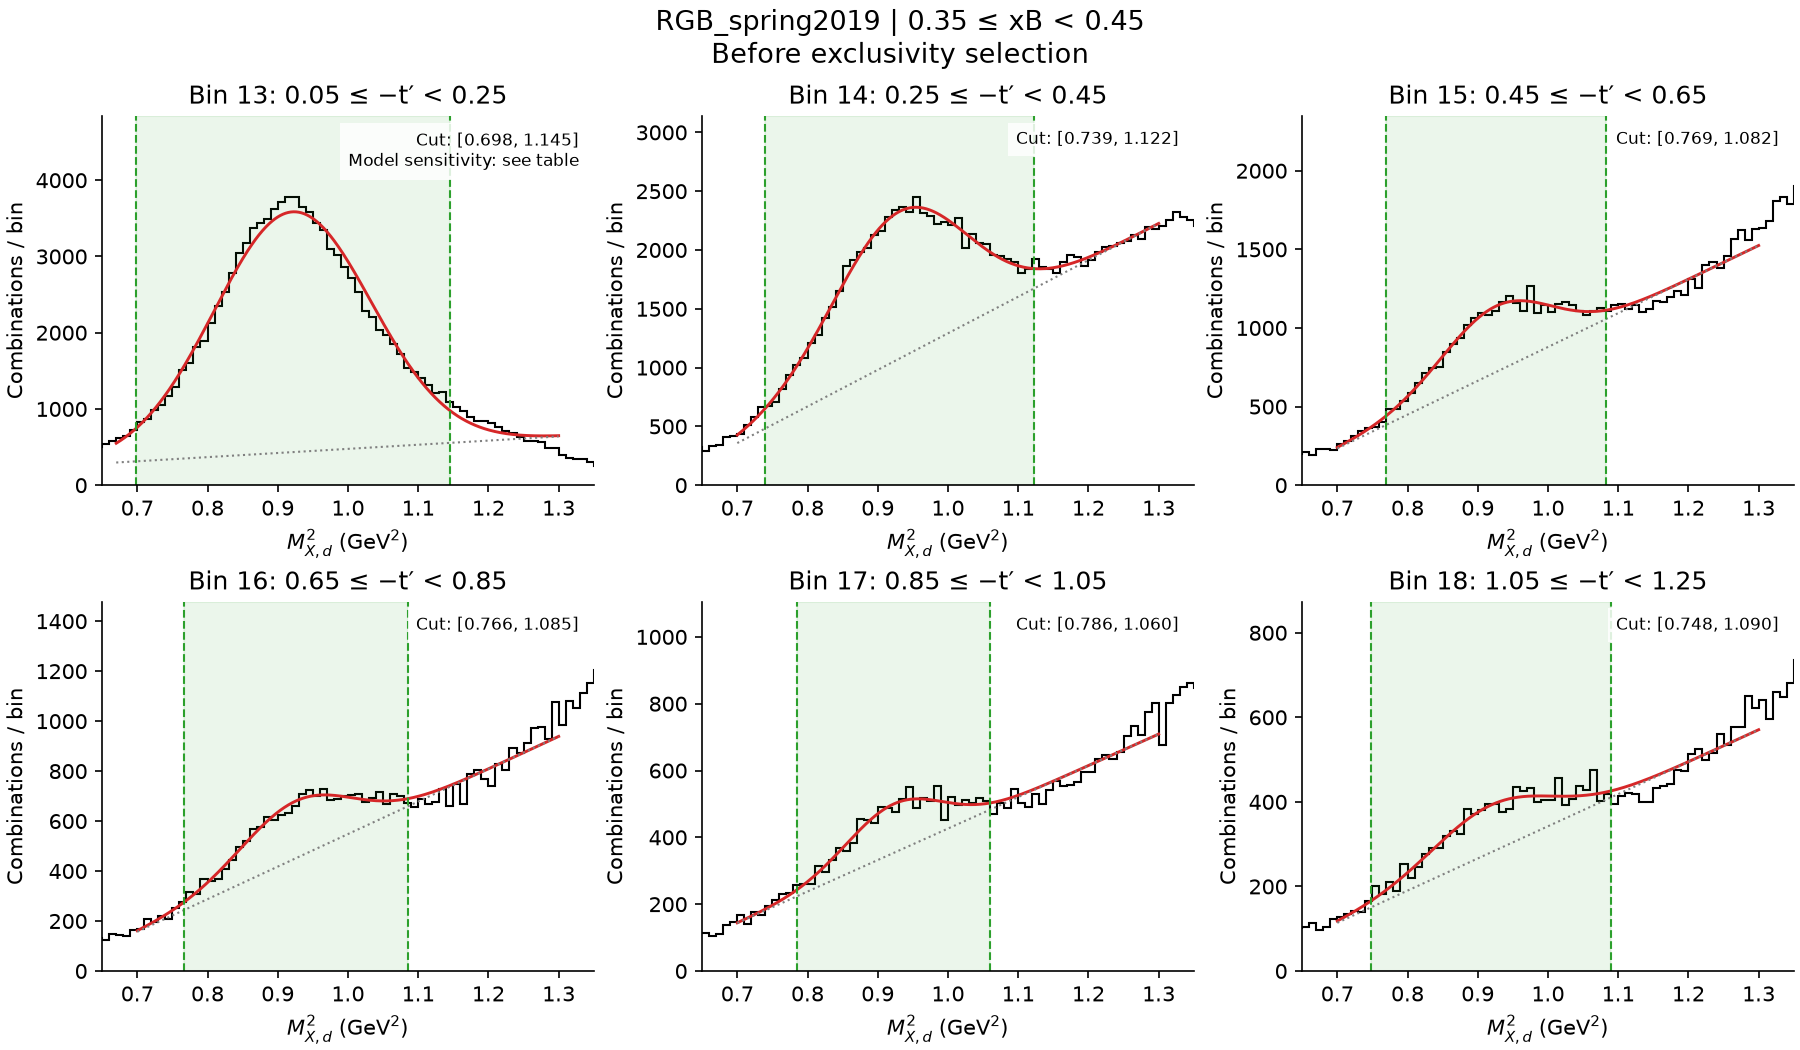
\includegraphics[width=\linewidth]{figures/channel_selection/exclusivity/rgb_sp19_mass_xb3.png}
\caption{RGB\_spring2019: deuteron-reference missing-mass-squared fits in $x_B$ interval 3. The panels retain the six fine selection bins.}\label{fig:new_excl_rgb_sp19_mass3}
\end{figure}
\clearpage
\begin{figure}[p]\centering
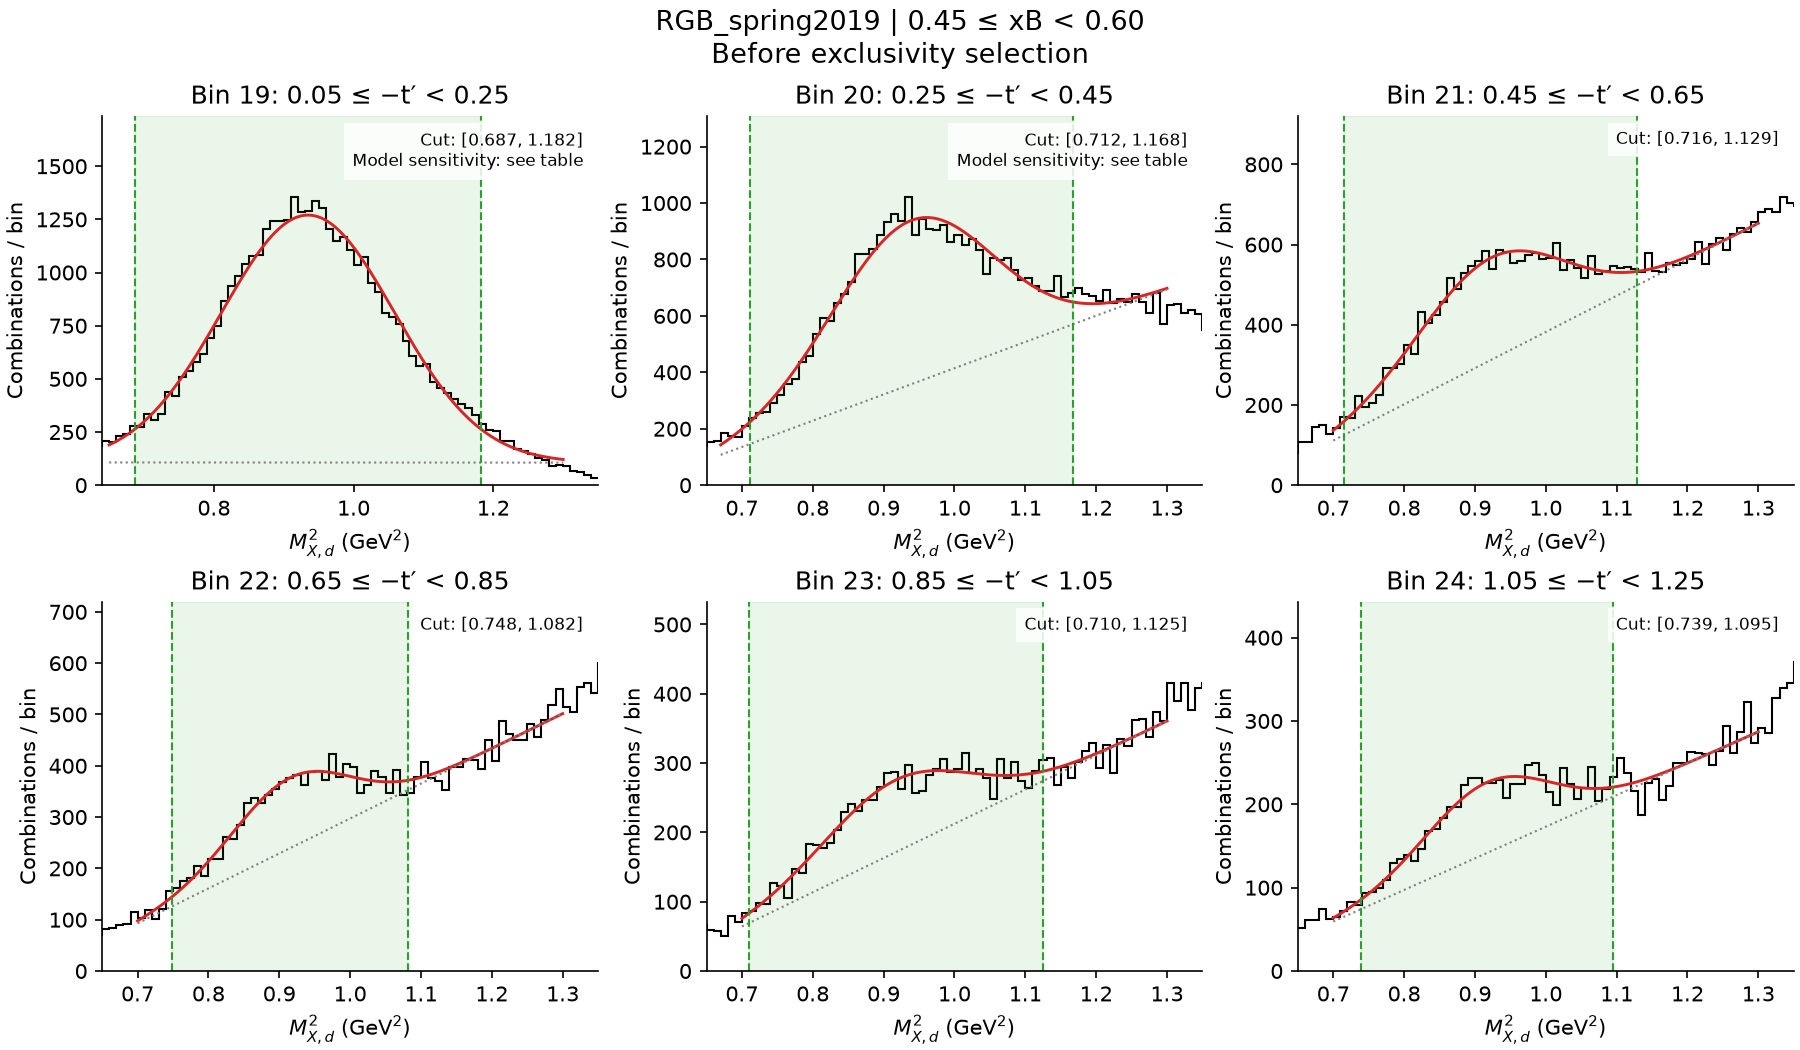
\includegraphics[width=\linewidth]{figures/channel_selection/exclusivity/rgb_sp19_mass_xb4.png}
\caption{RGB\_spring2019: deuteron-reference missing-mass-squared fits in $x_B$ interval 4. The panels retain the six fine selection bins.}\label{fig:new_excl_rgb_sp19_mass4}
\end{figure}
\clearpage
\begin{figure}[p]\centering
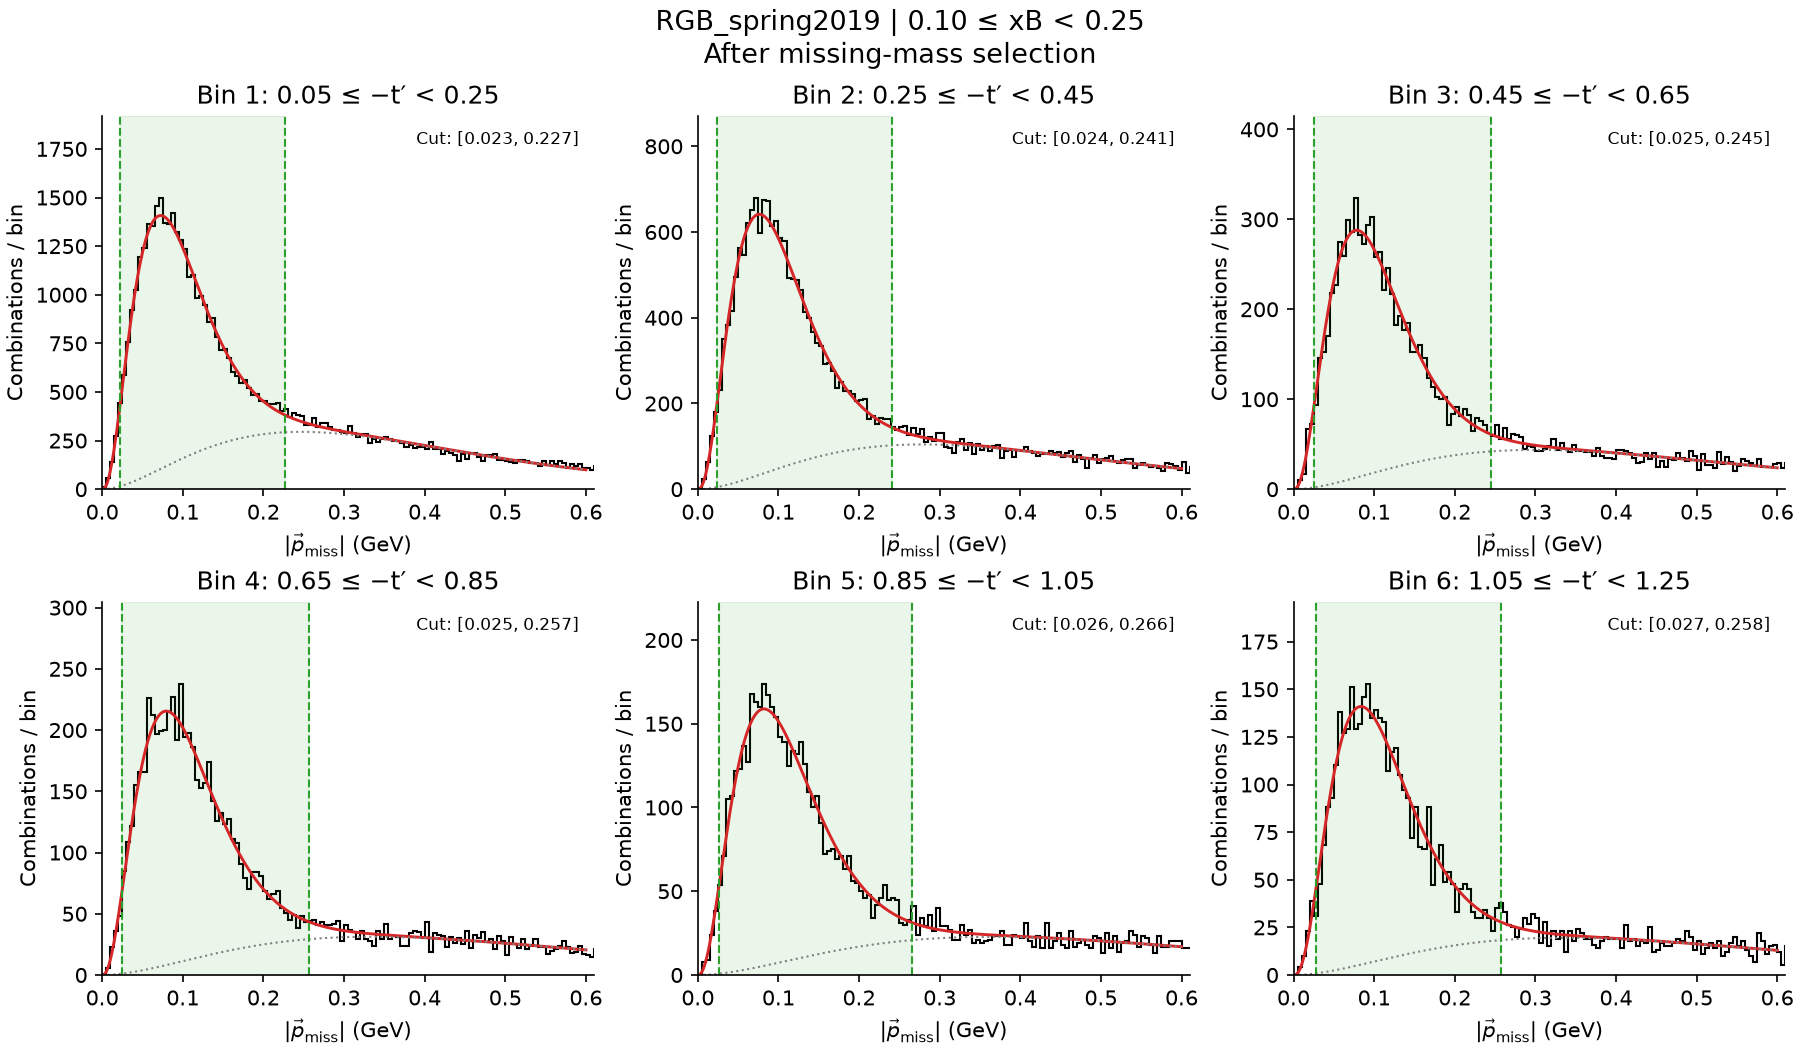
\includegraphics[width=\linewidth]{figures/channel_selection/exclusivity/rgb_sp19_momentum_xb1.png}
\caption{RGB\_spring2019: missing-momentum fits after the mass cut in $x_B$ interval 1. The panels retain the six fine selection bins.}\label{fig:new_excl_rgb_sp19_momentum1}
\end{figure}
\clearpage
\begin{figure}[p]\centering
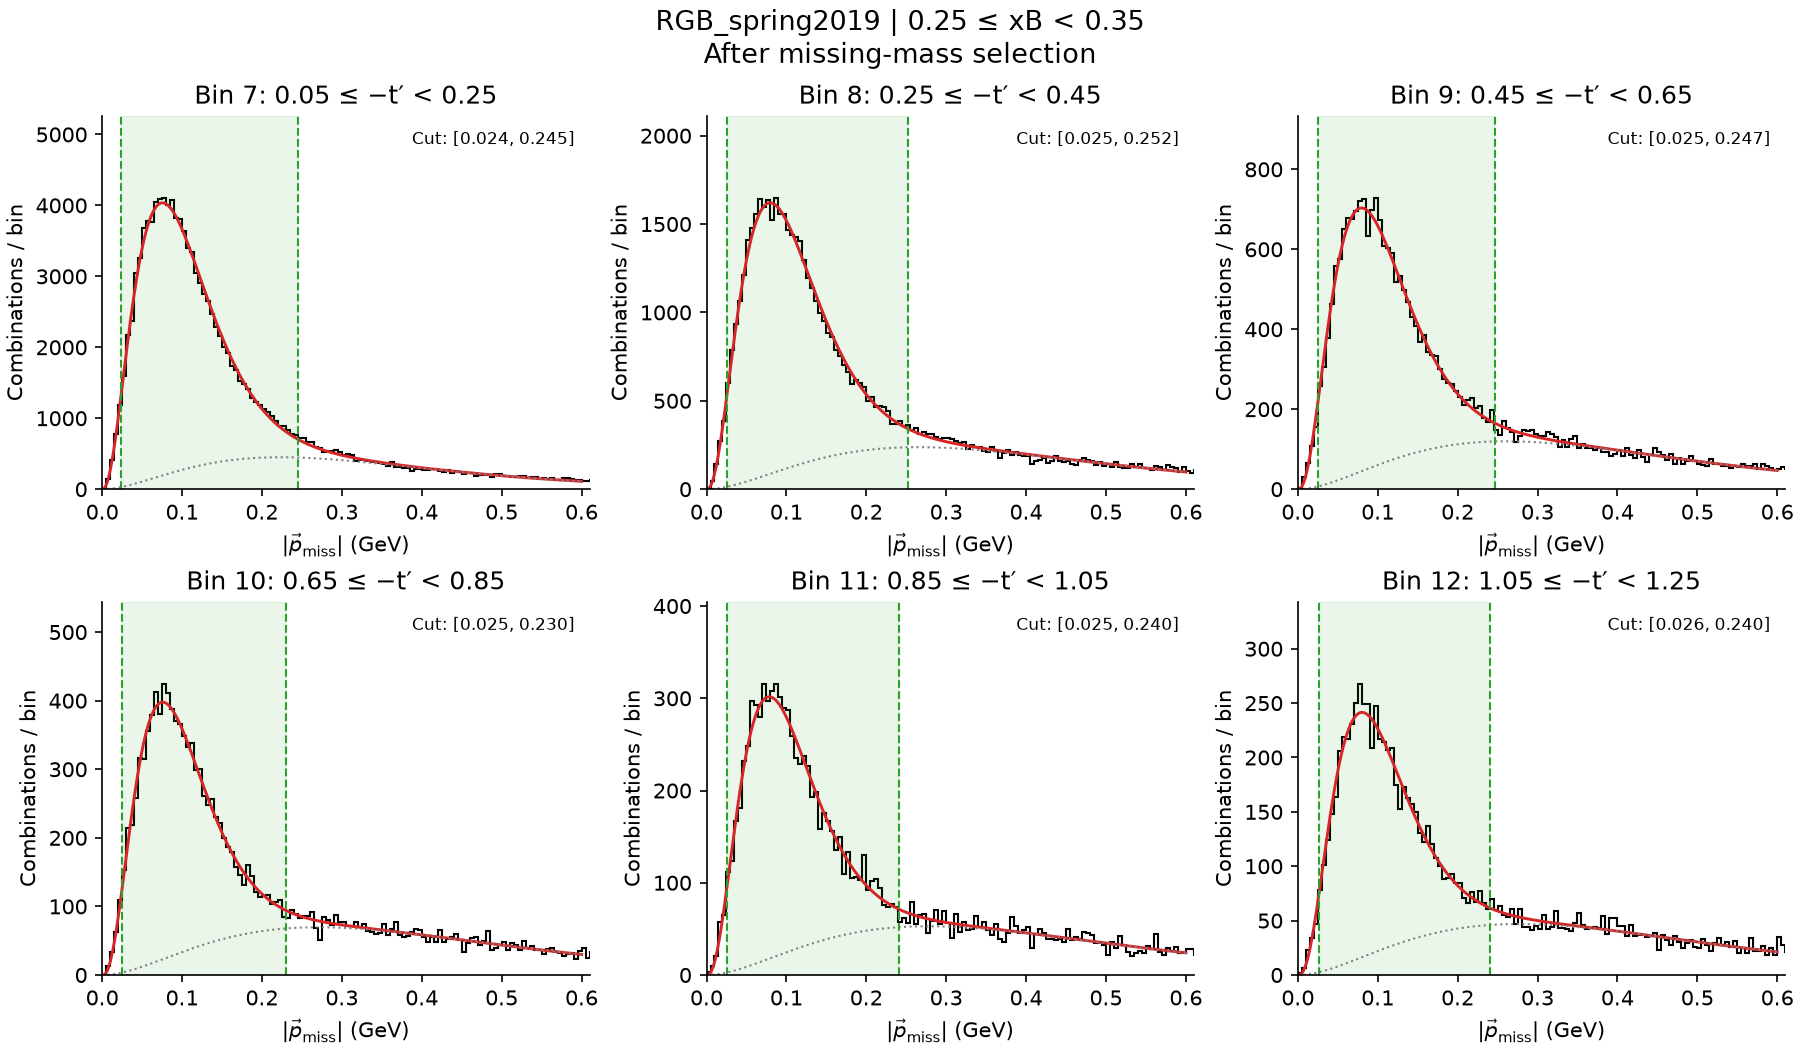
\includegraphics[width=\linewidth]{figures/channel_selection/exclusivity/rgb_sp19_momentum_xb2.png}
\caption{RGB\_spring2019: missing-momentum fits after the mass cut in $x_B$ interval 2. The panels retain the six fine selection bins.}\label{fig:new_excl_rgb_sp19_momentum2}
\end{figure}
\clearpage
\begin{figure}[p]\centering
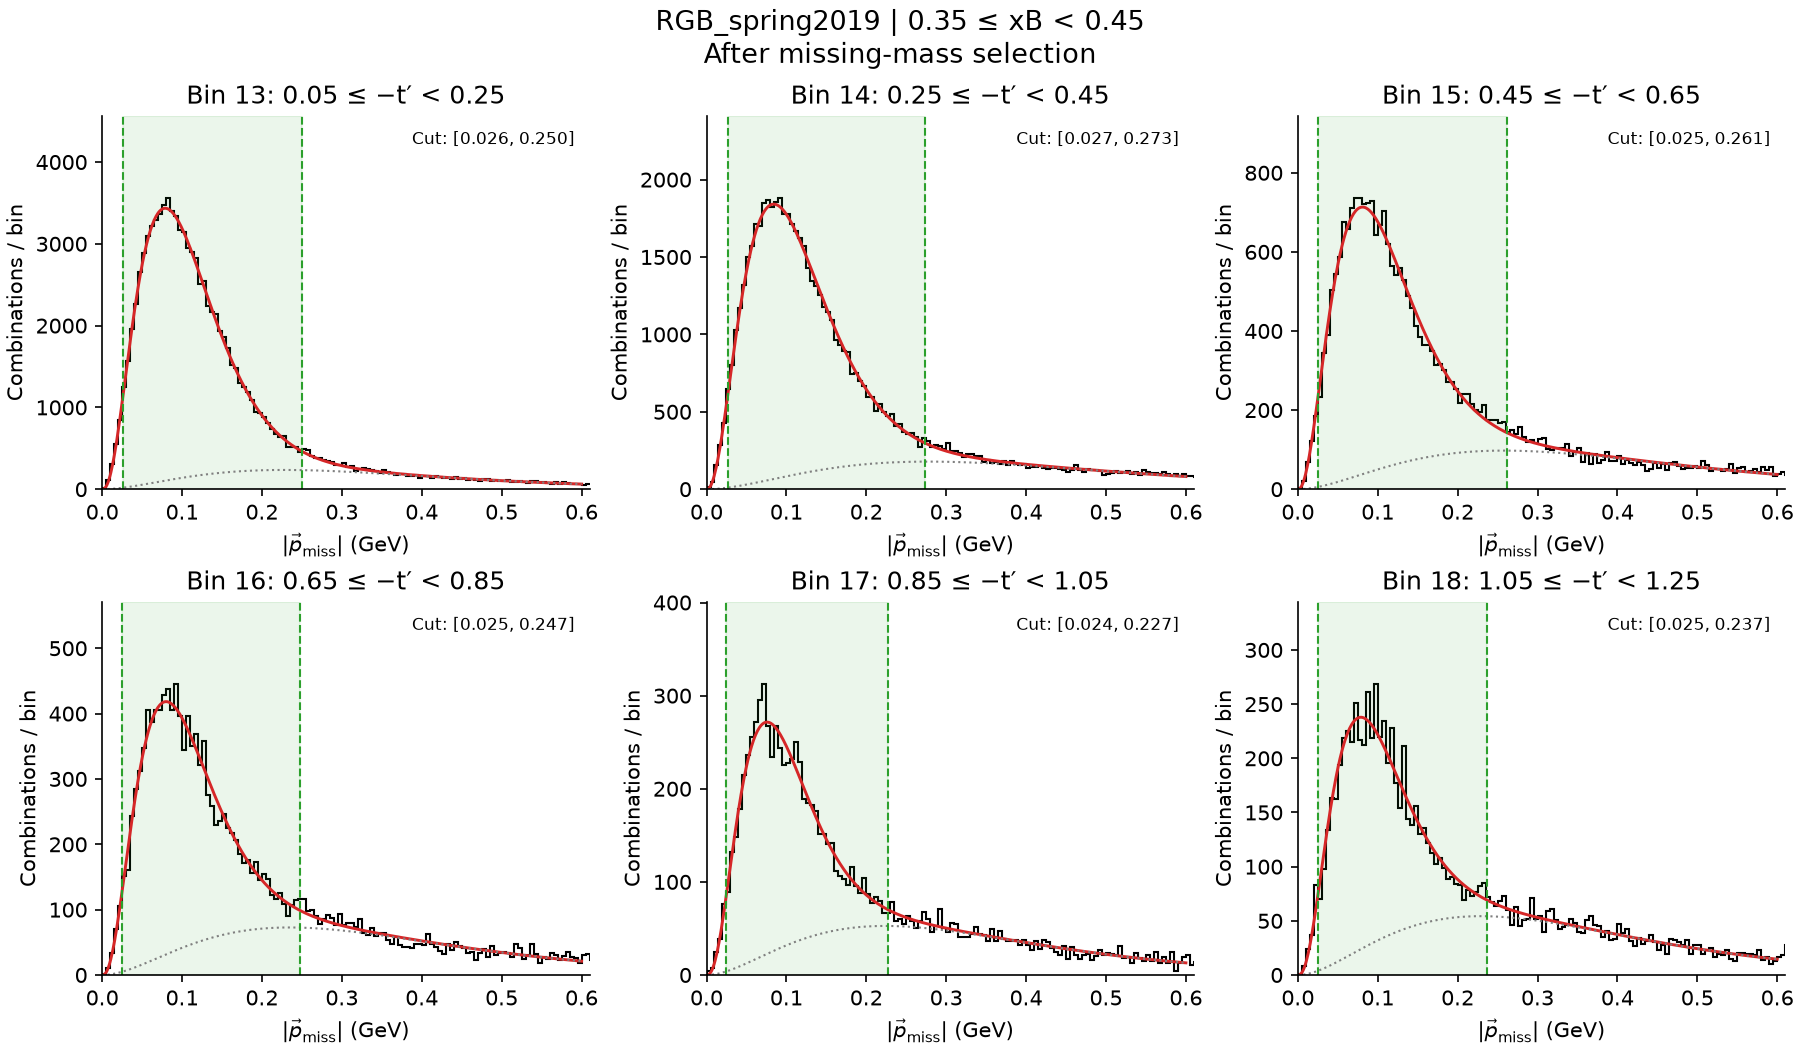
\includegraphics[width=\linewidth]{figures/channel_selection/exclusivity/rgb_sp19_momentum_xb3.png}
\caption{RGB\_spring2019: missing-momentum fits after the mass cut in $x_B$ interval 3. The panels retain the six fine selection bins.}\label{fig:new_excl_rgb_sp19_momentum3}
\end{figure}
\clearpage
\begin{figure}[p]\centering
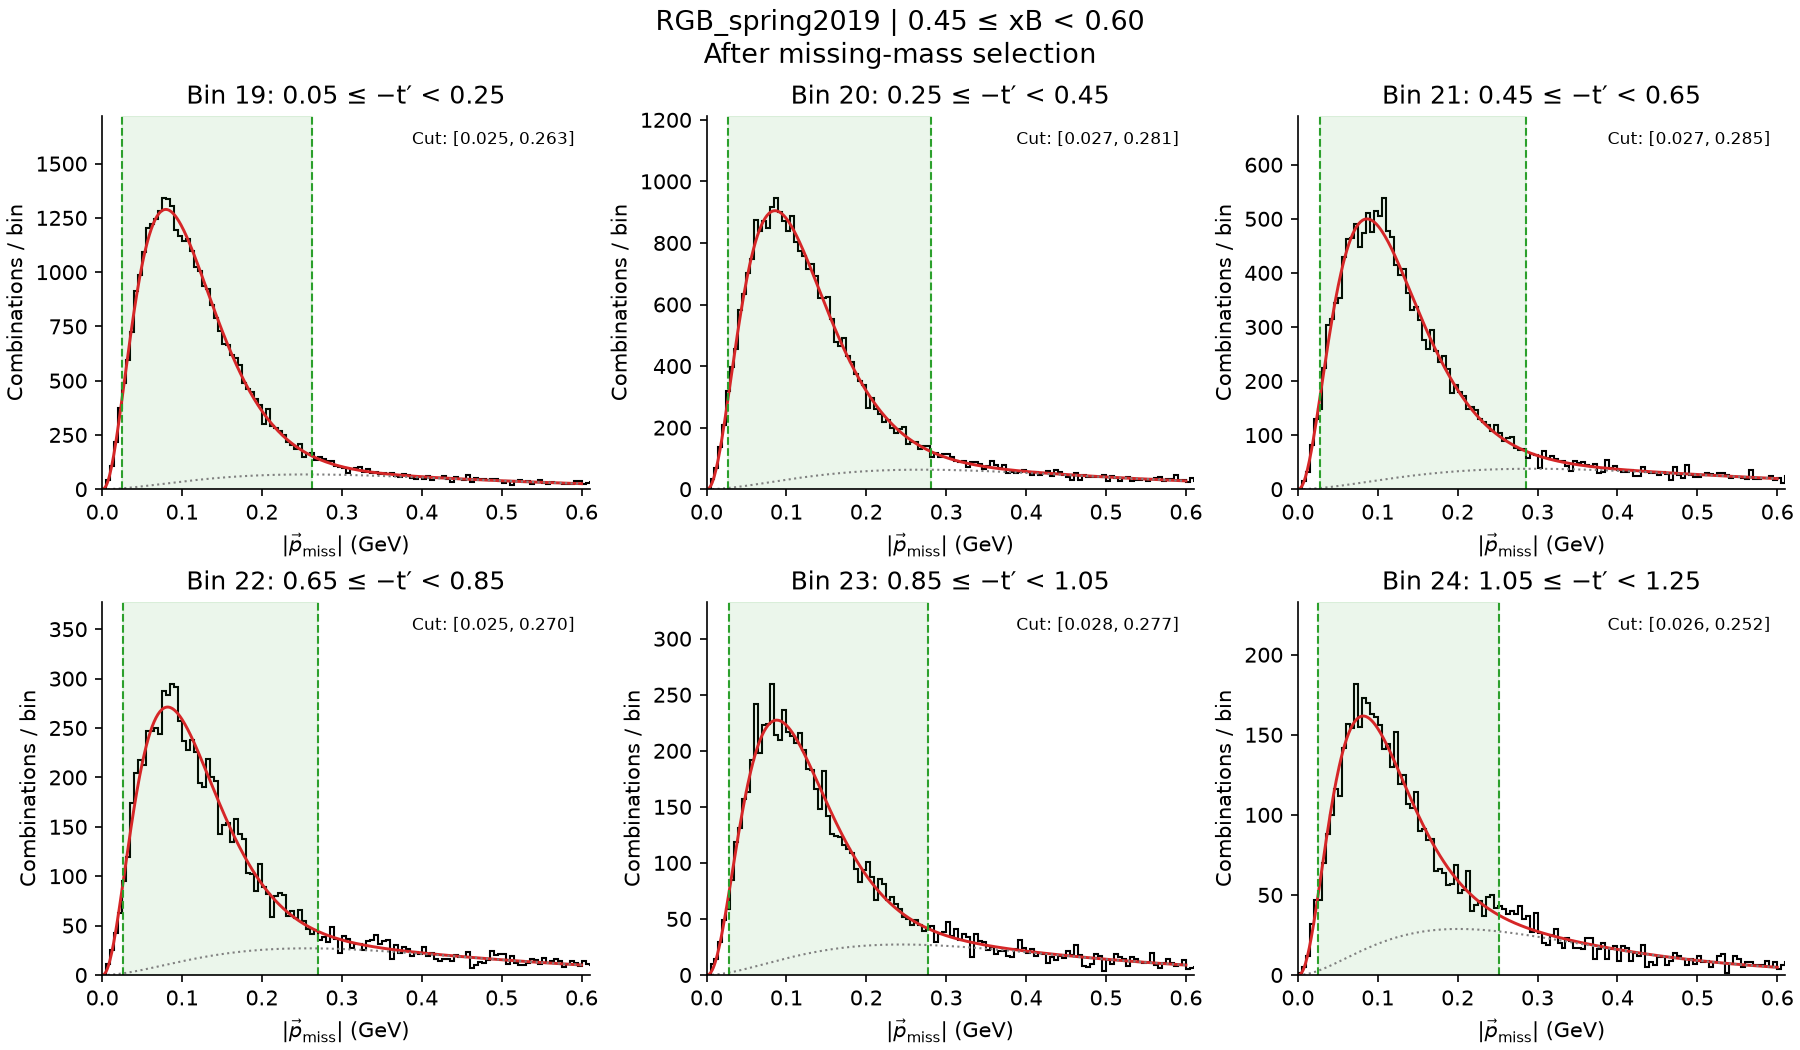
\includegraphics[width=\linewidth]{figures/channel_selection/exclusivity/rgb_sp19_momentum_xb4.png}
\caption{RGB\_spring2019: missing-momentum fits after the mass cut in $x_B$ interval 4. The panels retain the six fine selection bins.}\label{fig:new_excl_rgb_sp19_momentum4}
\end{figure}
\clearpage
\begin{figure}[p]\centering
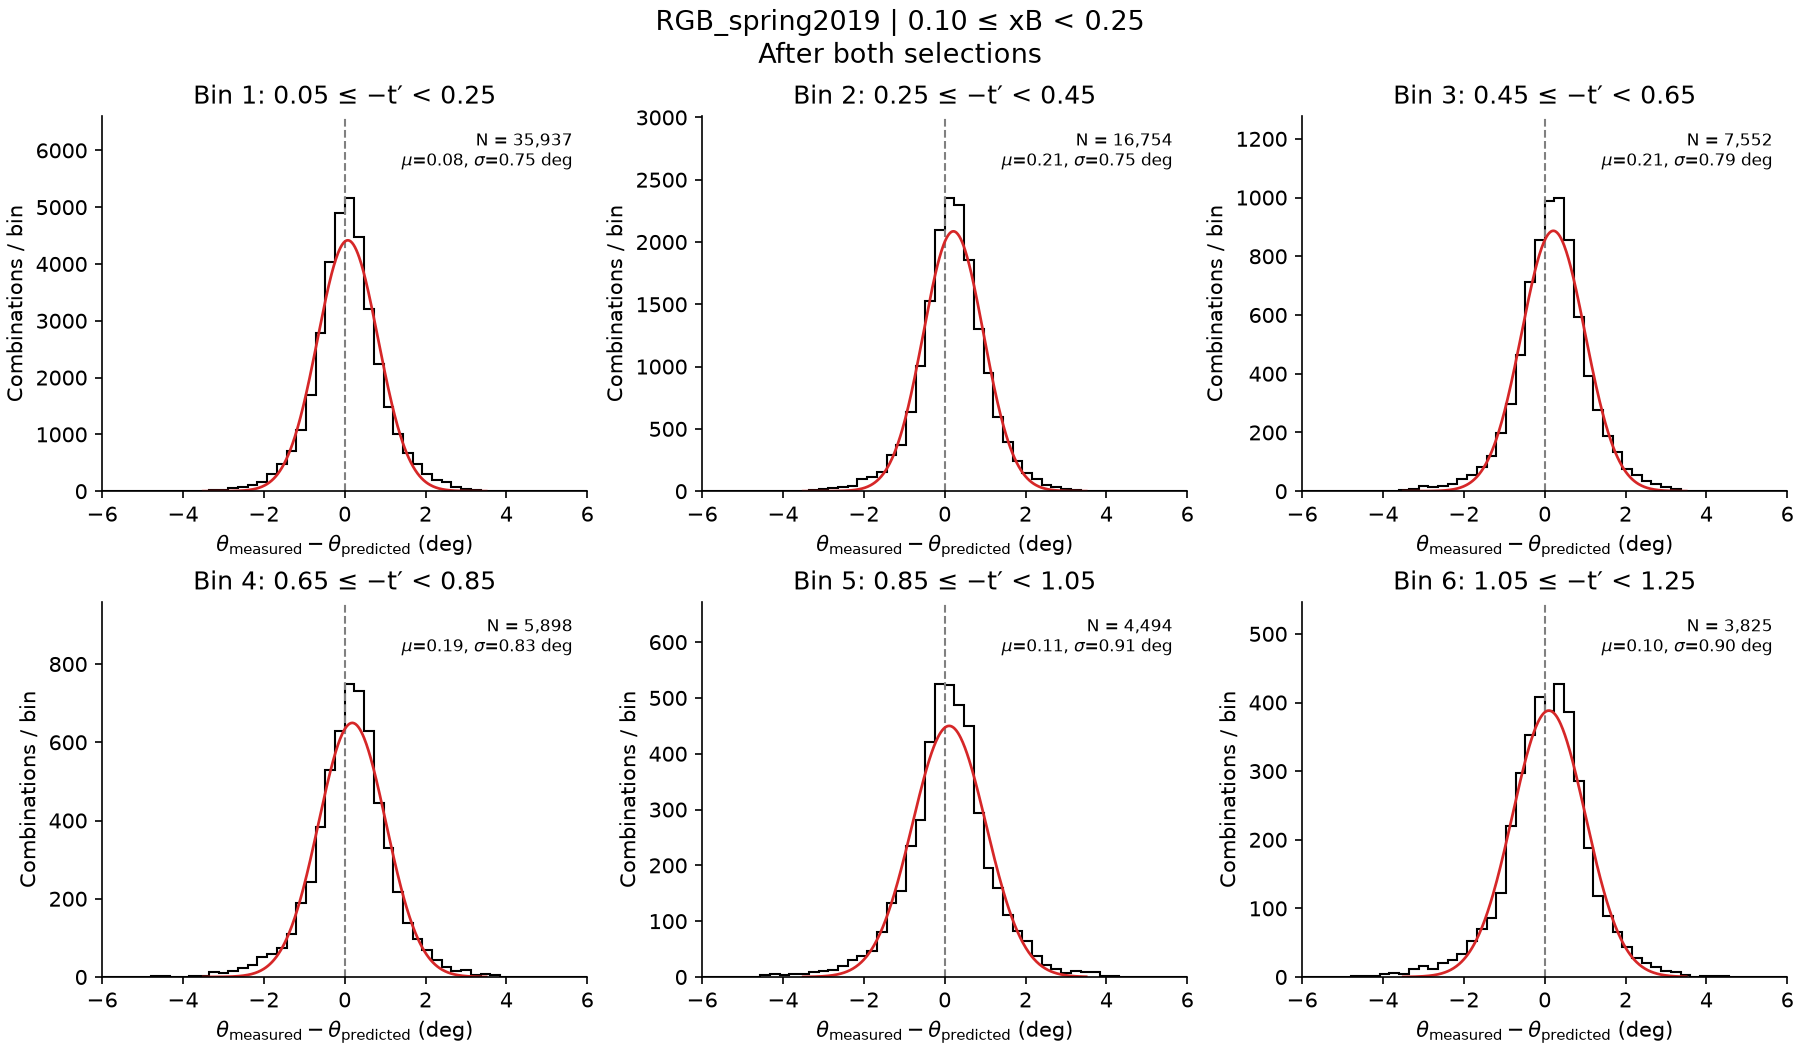
\includegraphics[width=\linewidth]{figures/channel_selection/exclusivity/rgb_sp19_angle_xb1.png}
\caption{RGB\_spring2019: pion polar-angle closure after both cuts in $x_B$ interval 1. The panels retain the six fine selection bins.}\label{fig:new_excl_rgb_sp19_angle1}
\end{figure}
\clearpage
\begin{figure}[p]\centering
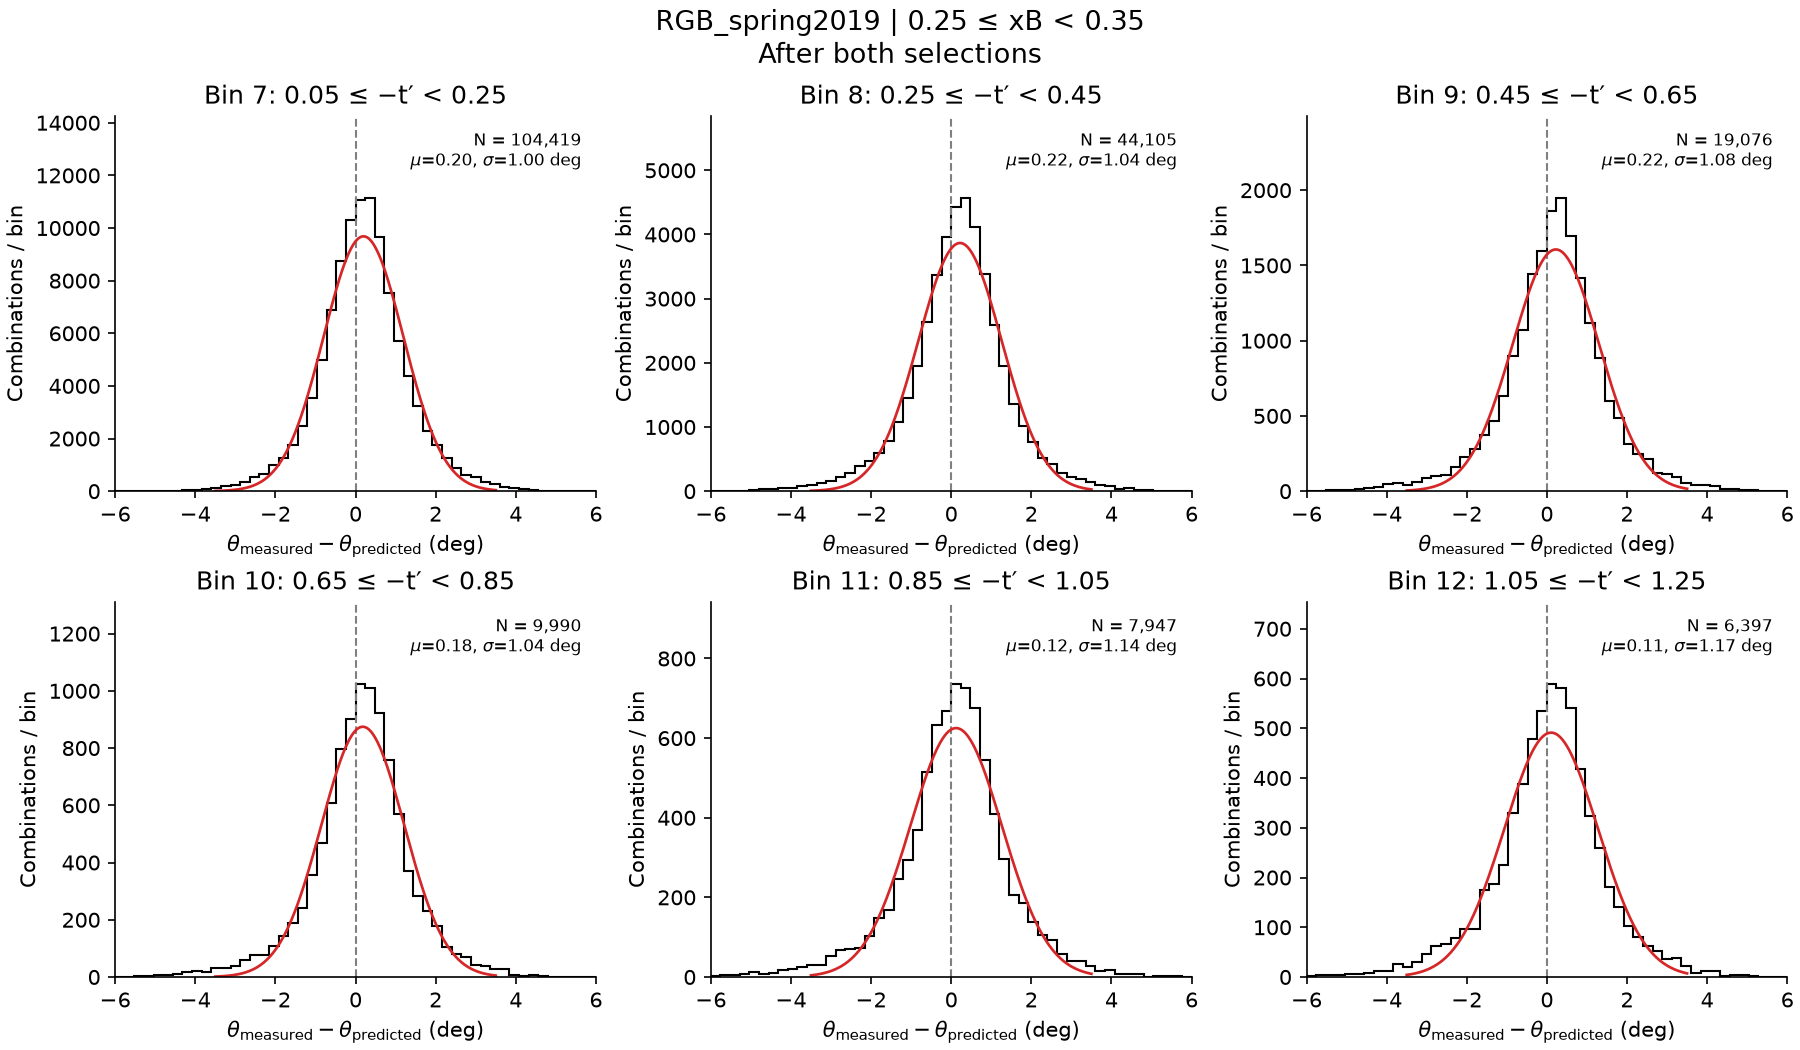
\includegraphics[width=\linewidth]{figures/channel_selection/exclusivity/rgb_sp19_angle_xb2.png}
\caption{RGB\_spring2019: pion polar-angle closure after both cuts in $x_B$ interval 2. The panels retain the six fine selection bins.}\label{fig:new_excl_rgb_sp19_angle2}
\end{figure}
\clearpage
\begin{figure}[p]\centering
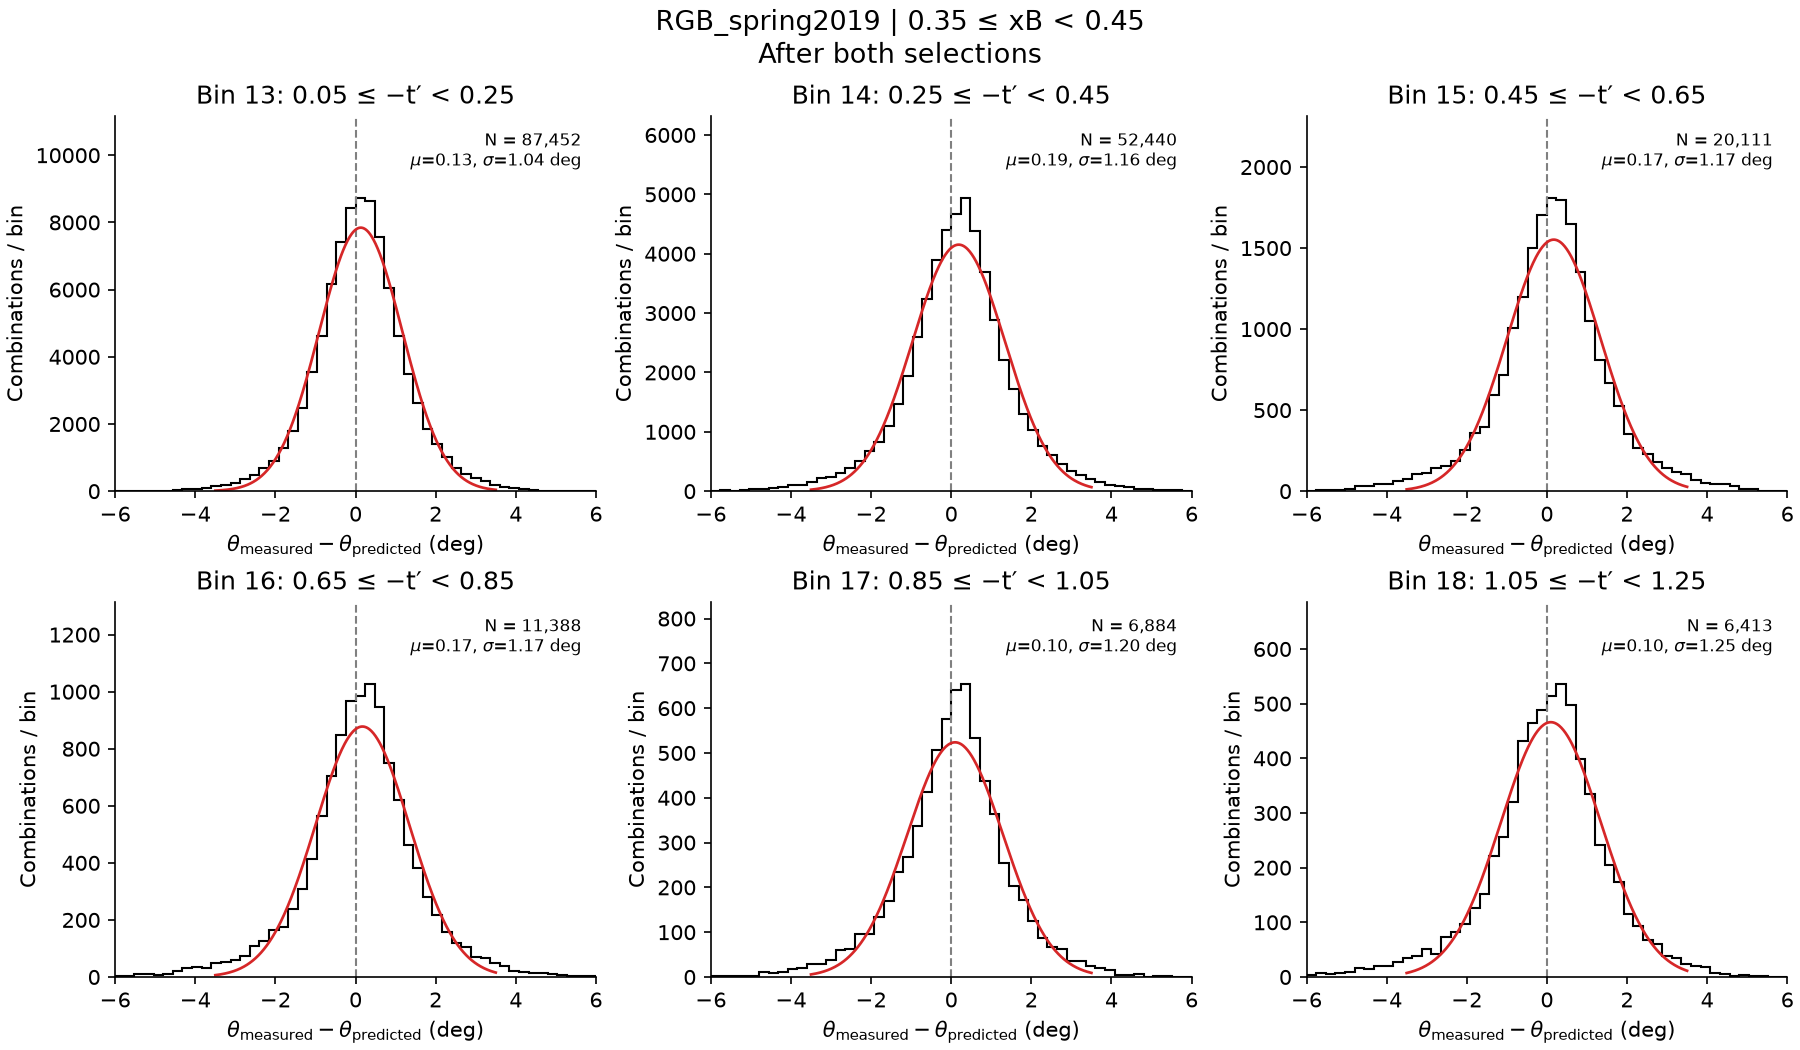
\includegraphics[width=\linewidth]{figures/channel_selection/exclusivity/rgb_sp19_angle_xb3.png}
\caption{RGB\_spring2019: pion polar-angle closure after both cuts in $x_B$ interval 3. The panels retain the six fine selection bins.}\label{fig:new_excl_rgb_sp19_angle3}
\end{figure}
\clearpage
\begin{figure}[p]\centering
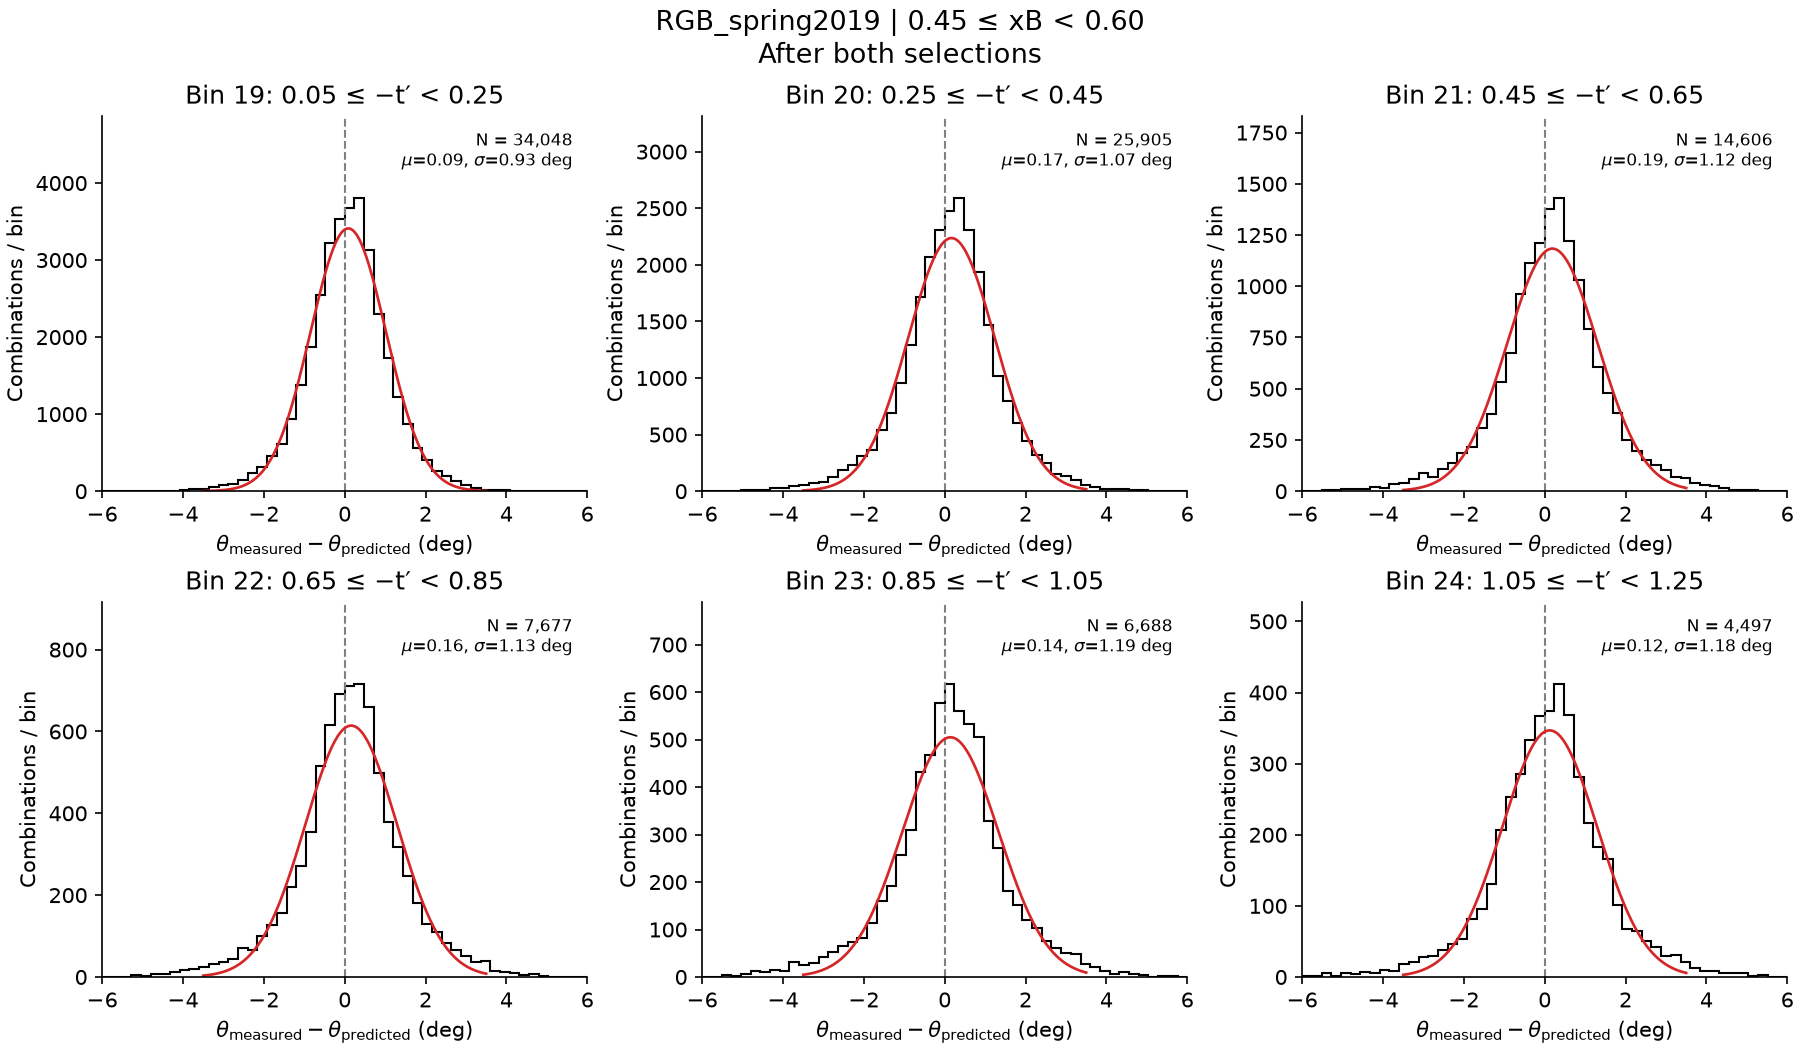
\includegraphics[width=\linewidth]{figures/channel_selection/exclusivity/rgb_sp19_angle_xb4.png}
\caption{RGB\_spring2019: pion polar-angle closure after both cuts in $x_B$ interval 4. The panels retain the six fine selection bins.}\label{fig:new_excl_rgb_sp19_angle4}
\end{figure}
\clearpage
\begin{figure}[p]\centering
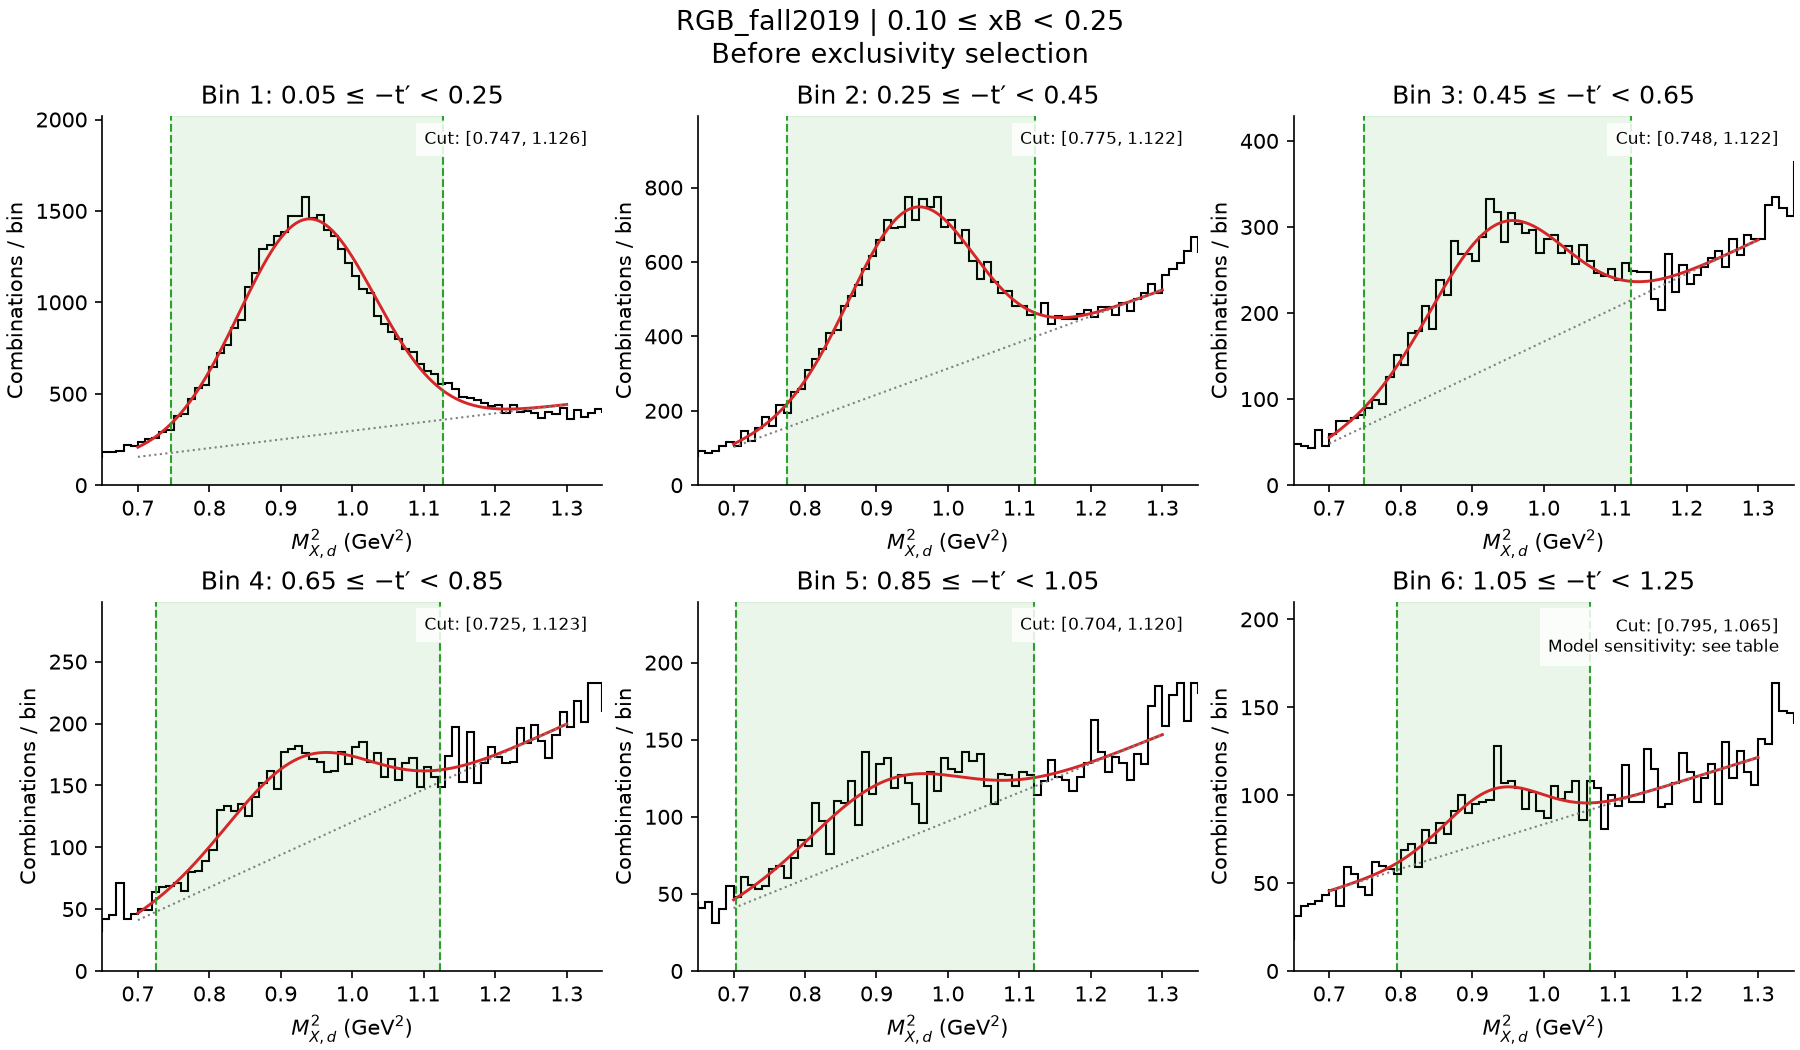
\includegraphics[width=\linewidth]{figures/channel_selection/exclusivity/rgb_fa19_mass_xb1.png}
\caption{RGB\_fall2019: deuteron-reference missing-mass-squared fits in $x_B$ interval 1. The panels retain the six fine selection bins.}\label{fig:new_excl_rgb_fa19_mass1}
\end{figure}
\clearpage
\begin{figure}[p]\centering
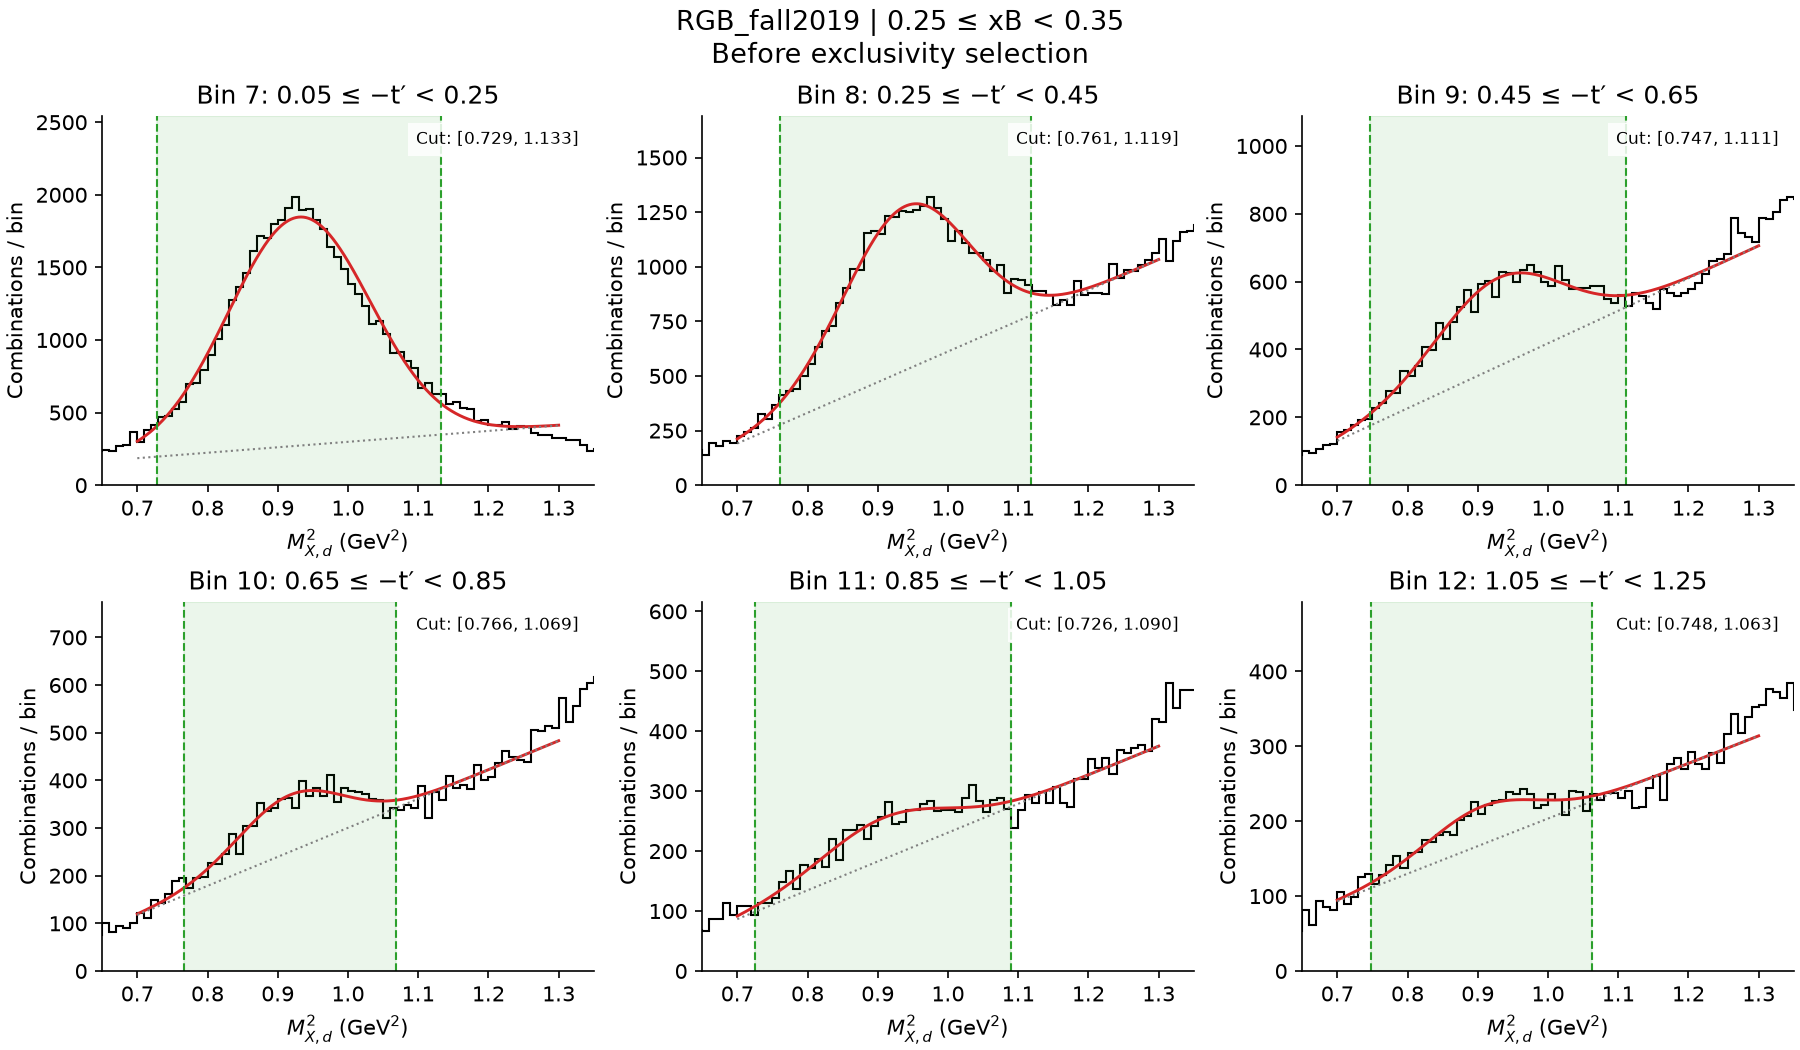
\includegraphics[width=\linewidth]{figures/channel_selection/exclusivity/rgb_fa19_mass_xb2.png}
\caption{RGB\_fall2019: deuteron-reference missing-mass-squared fits in $x_B$ interval 2. The panels retain the six fine selection bins.}\label{fig:new_excl_rgb_fa19_mass2}
\end{figure}
\clearpage
\begin{figure}[p]\centering
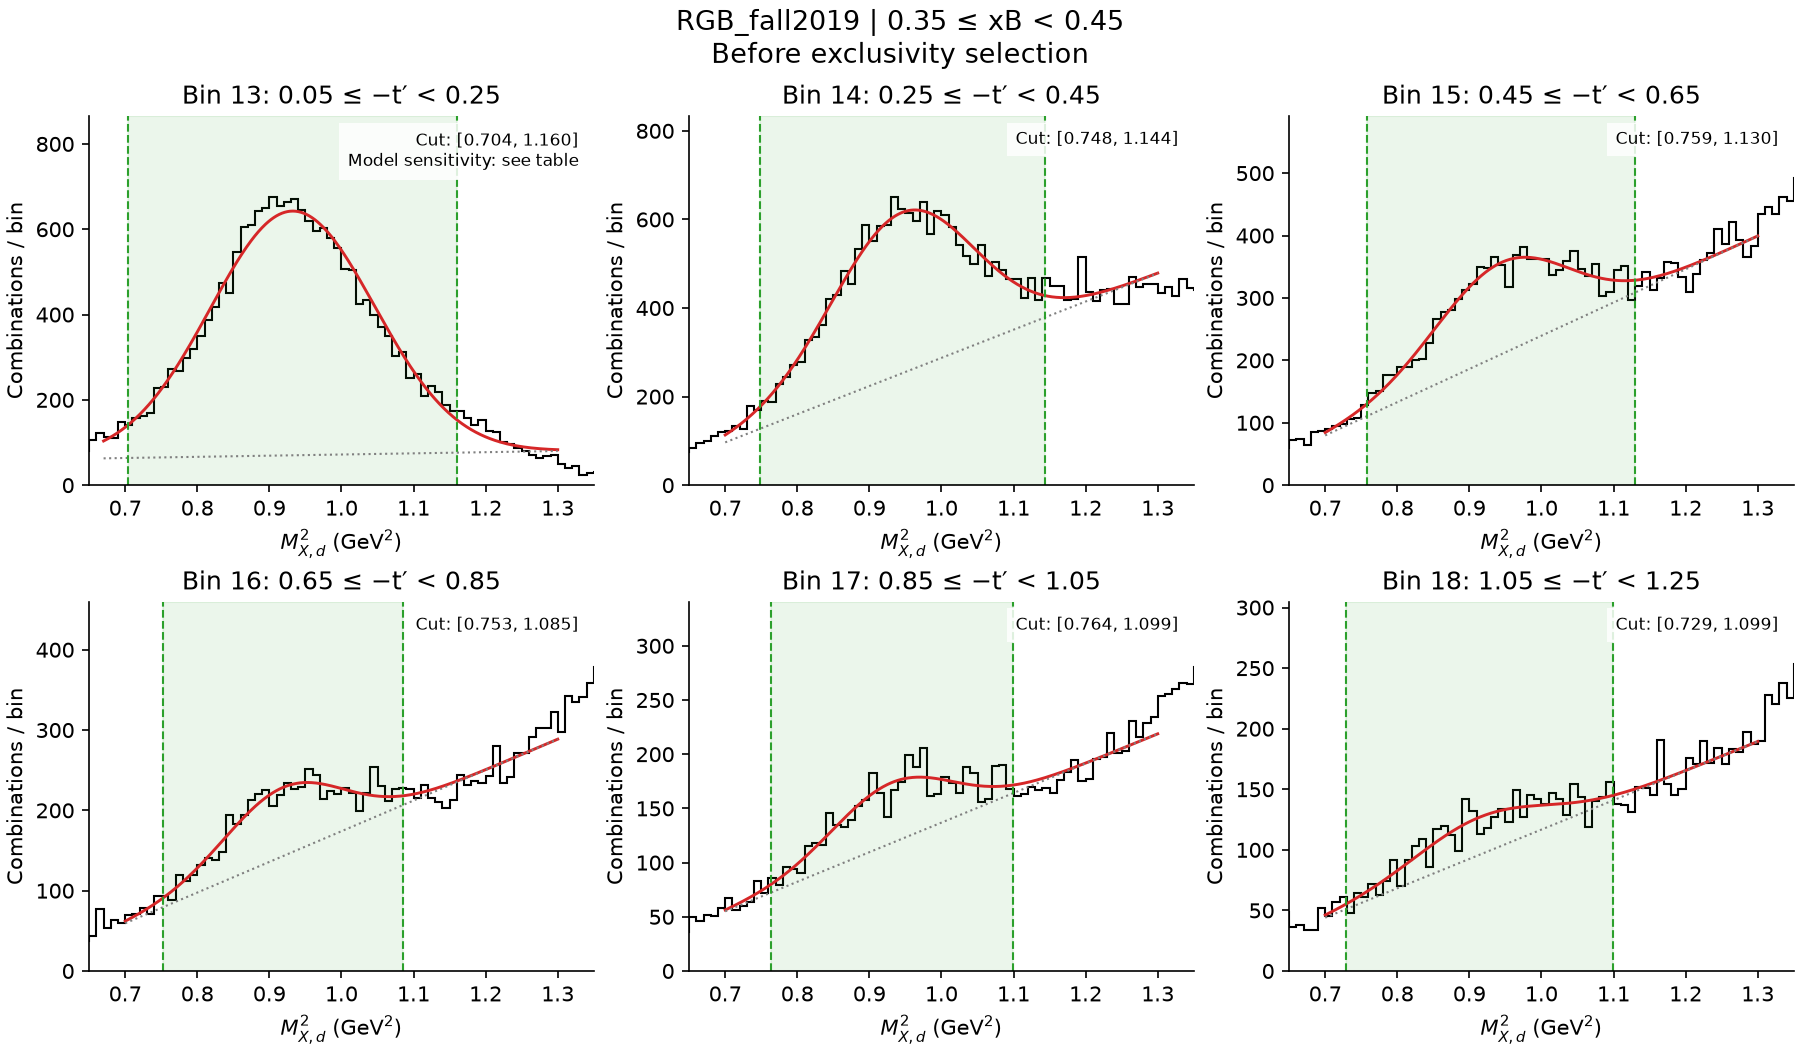
\includegraphics[width=\linewidth]{figures/channel_selection/exclusivity/rgb_fa19_mass_xb3.png}
\caption{RGB\_fall2019: deuteron-reference missing-mass-squared fits in $x_B$ interval 3. The panels retain the six fine selection bins.}\label{fig:new_excl_rgb_fa19_mass3}
\end{figure}
\clearpage
\begin{figure}[p]\centering
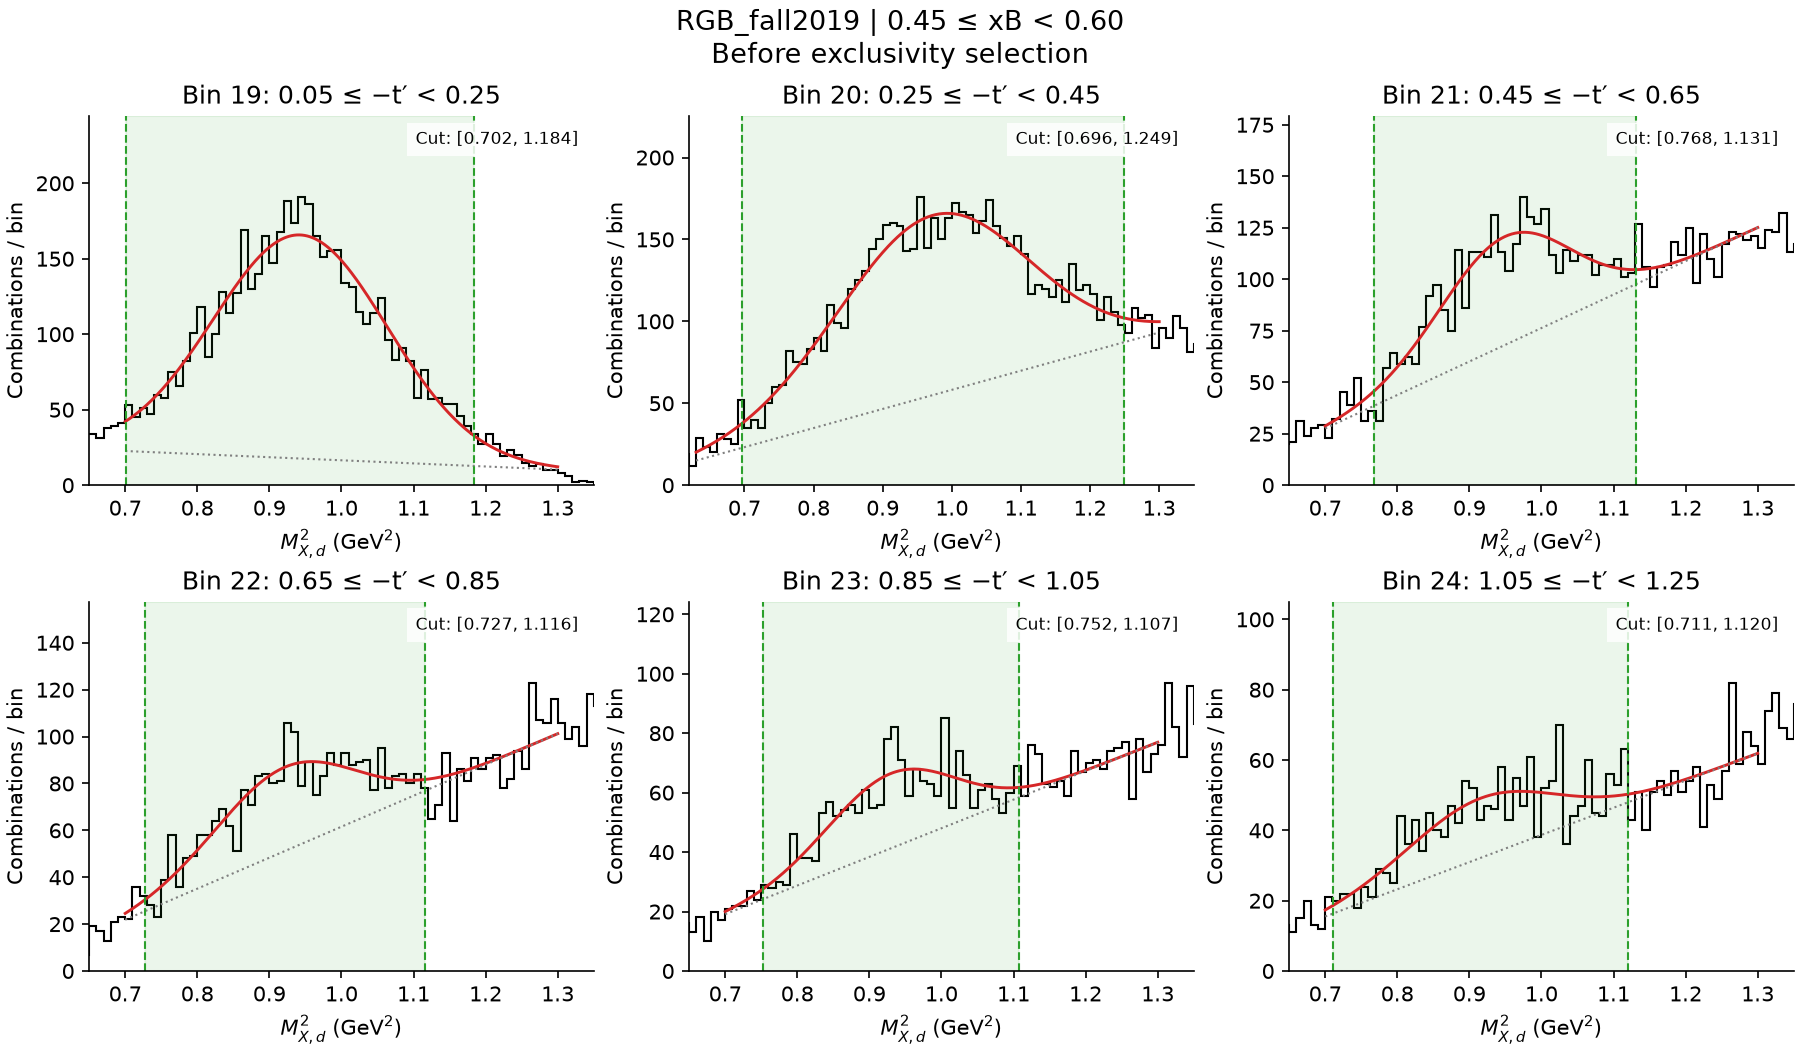
\includegraphics[width=\linewidth]{figures/channel_selection/exclusivity/rgb_fa19_mass_xb4.png}
\caption{RGB\_fall2019: deuteron-reference missing-mass-squared fits in $x_B$ interval 4. The panels retain the six fine selection bins.}\label{fig:new_excl_rgb_fa19_mass4}
\end{figure}
\clearpage
\begin{figure}[p]\centering
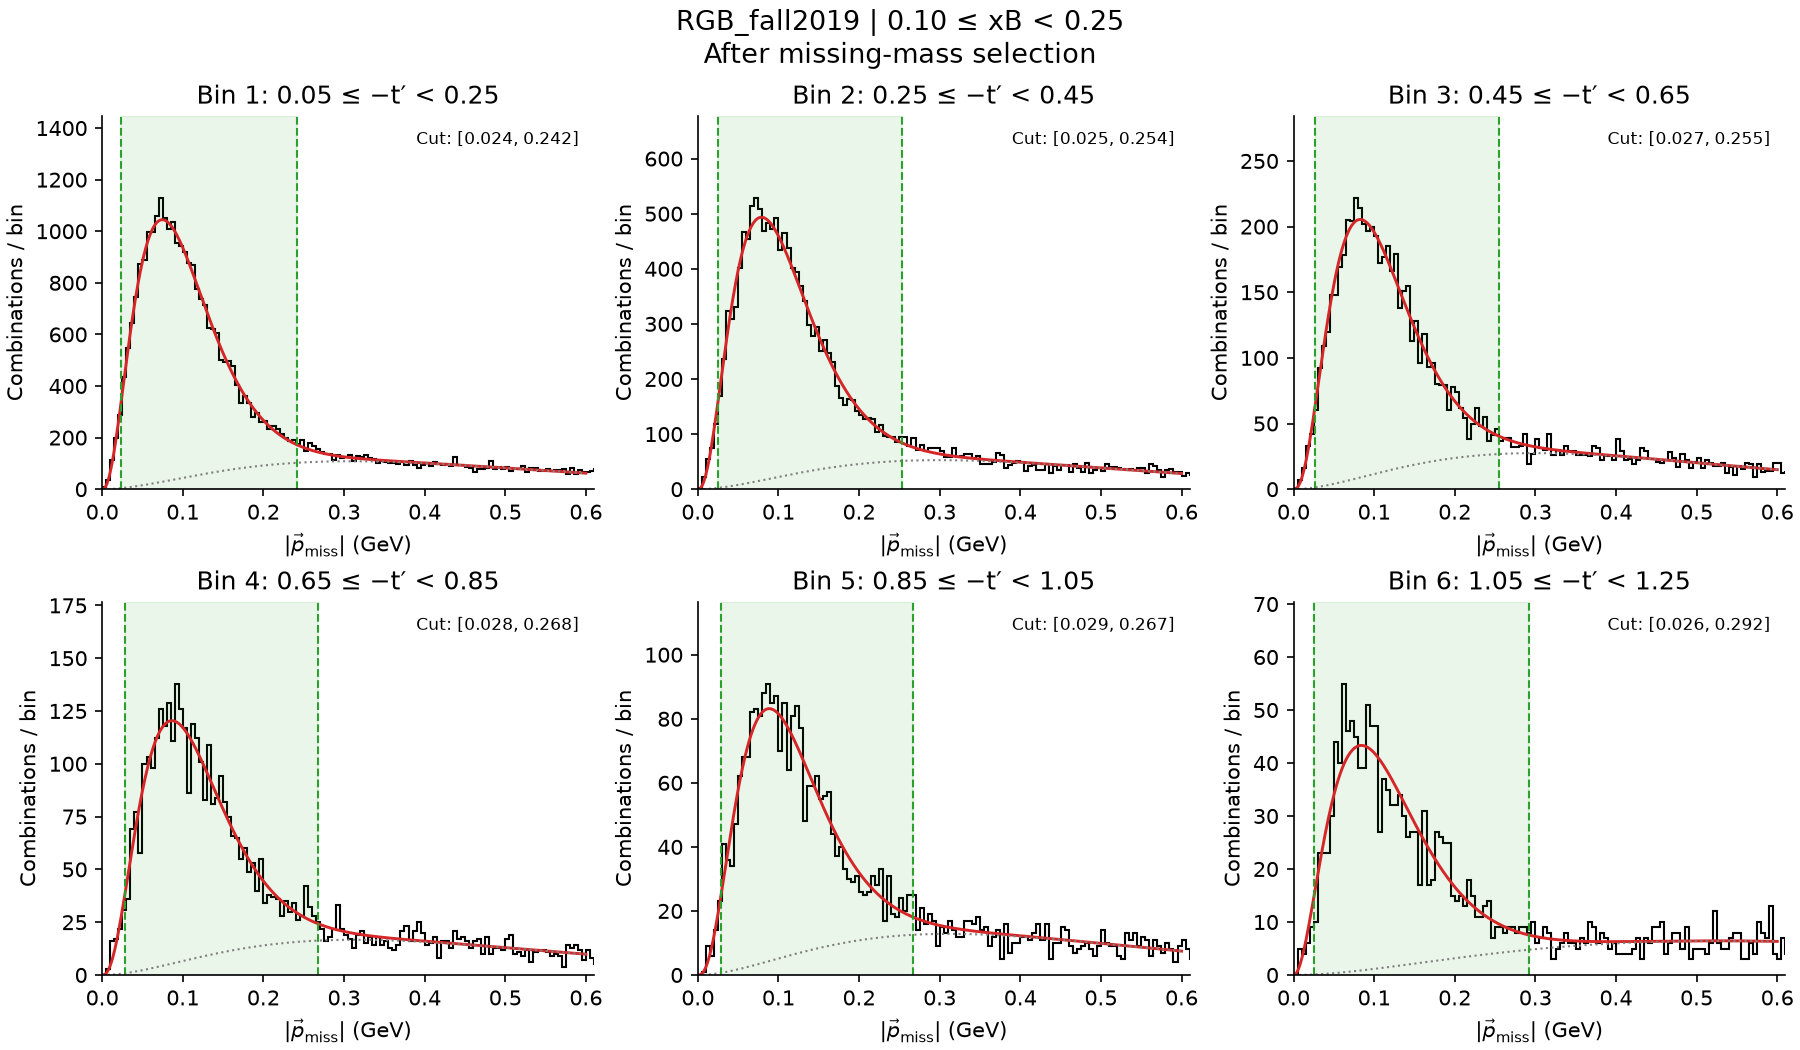
\includegraphics[width=\linewidth]{figures/channel_selection/exclusivity/rgb_fa19_momentum_xb1.png}
\caption{RGB\_fall2019: missing-momentum fits after the mass cut in $x_B$ interval 1. The panels retain the six fine selection bins.}\label{fig:new_excl_rgb_fa19_momentum1}
\end{figure}
\clearpage
\begin{figure}[p]\centering
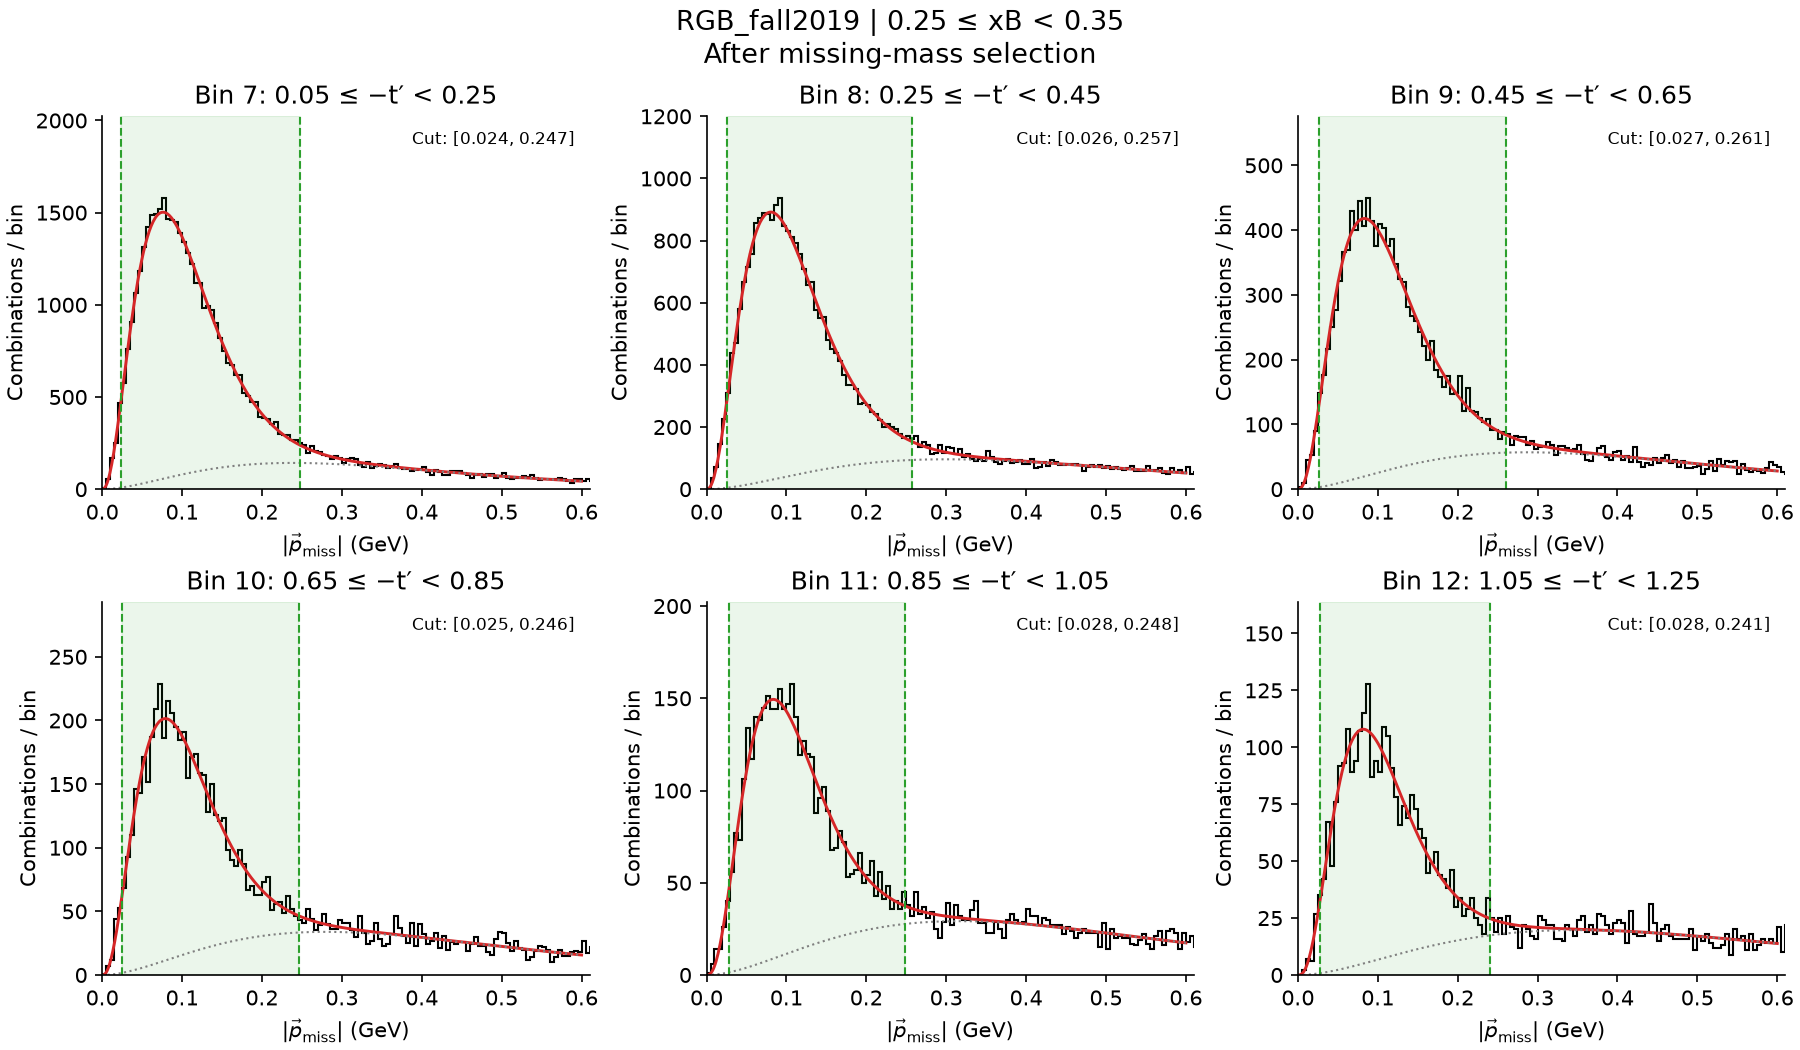
\includegraphics[width=\linewidth]{figures/channel_selection/exclusivity/rgb_fa19_momentum_xb2.png}
\caption{RGB\_fall2019: missing-momentum fits after the mass cut in $x_B$ interval 2. The panels retain the six fine selection bins.}\label{fig:new_excl_rgb_fa19_momentum2}
\end{figure}
\clearpage
\begin{figure}[p]\centering
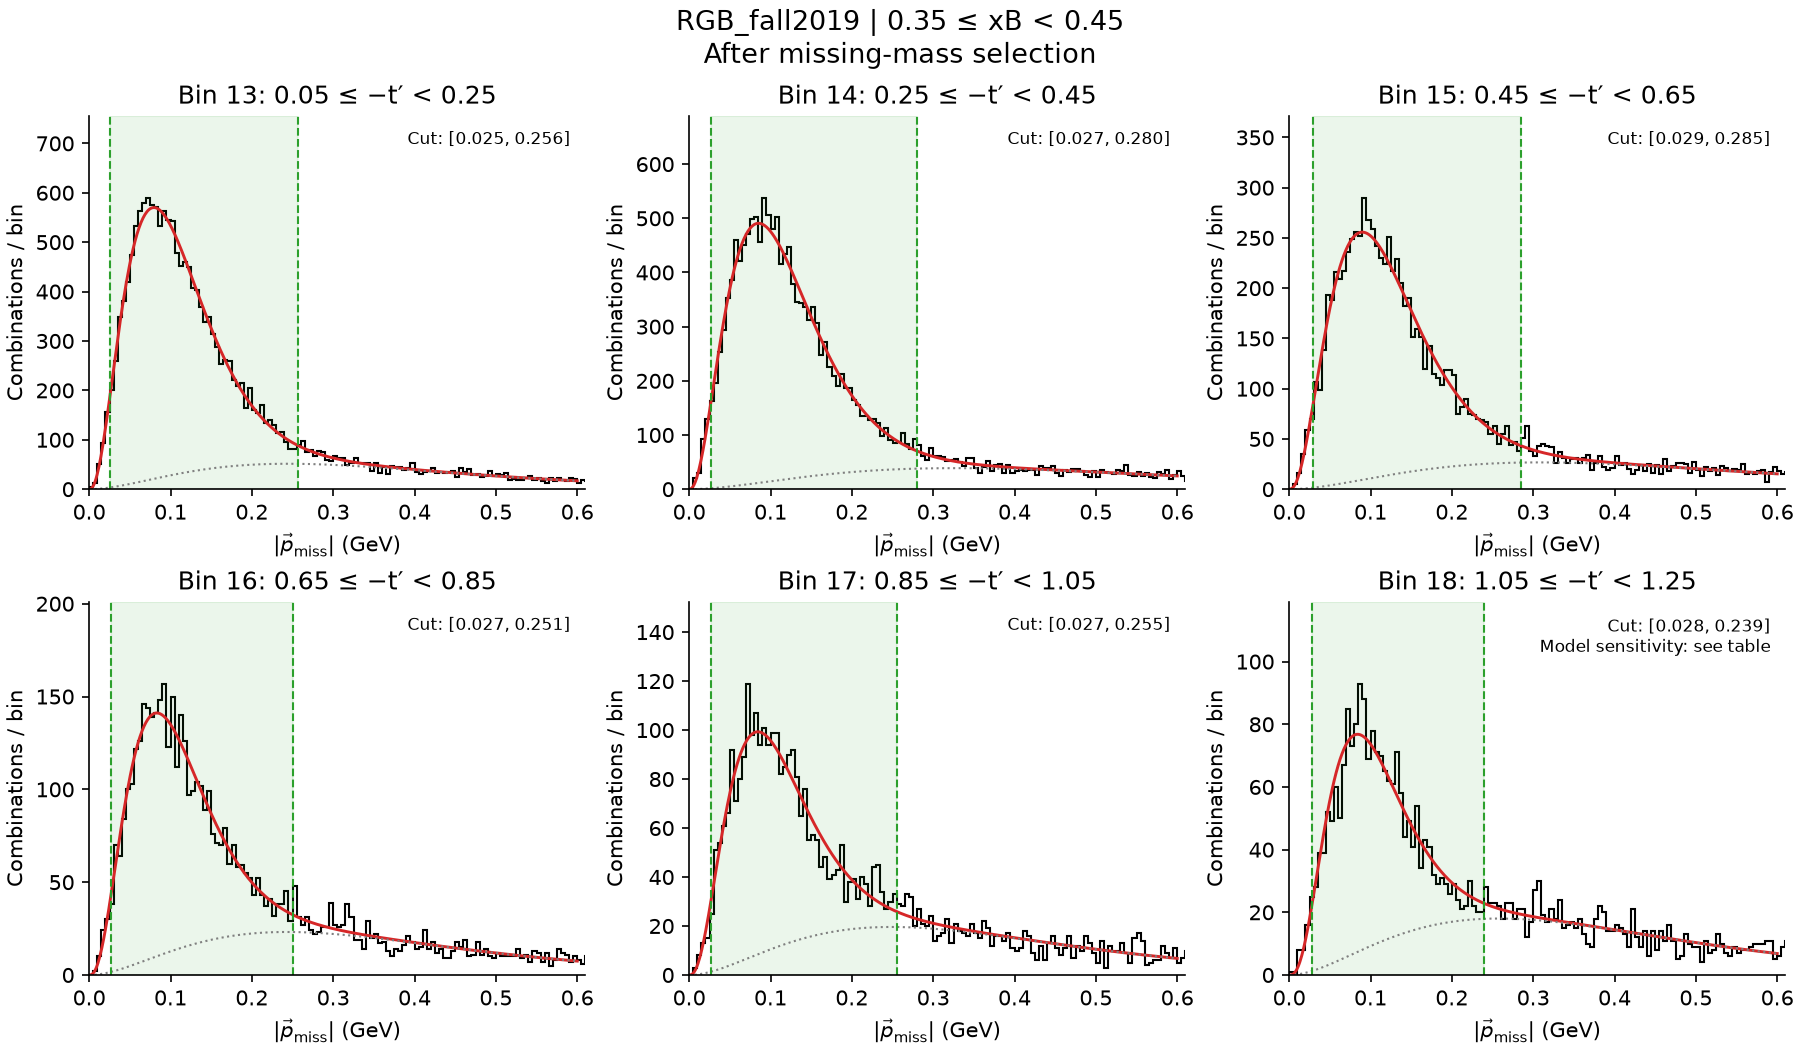
\includegraphics[width=\linewidth]{figures/channel_selection/exclusivity/rgb_fa19_momentum_xb3.png}
\caption{RGB\_fall2019: missing-momentum fits after the mass cut in $x_B$ interval 3. The panels retain the six fine selection bins.}\label{fig:new_excl_rgb_fa19_momentum3}
\end{figure}
\clearpage
\begin{figure}[p]\centering
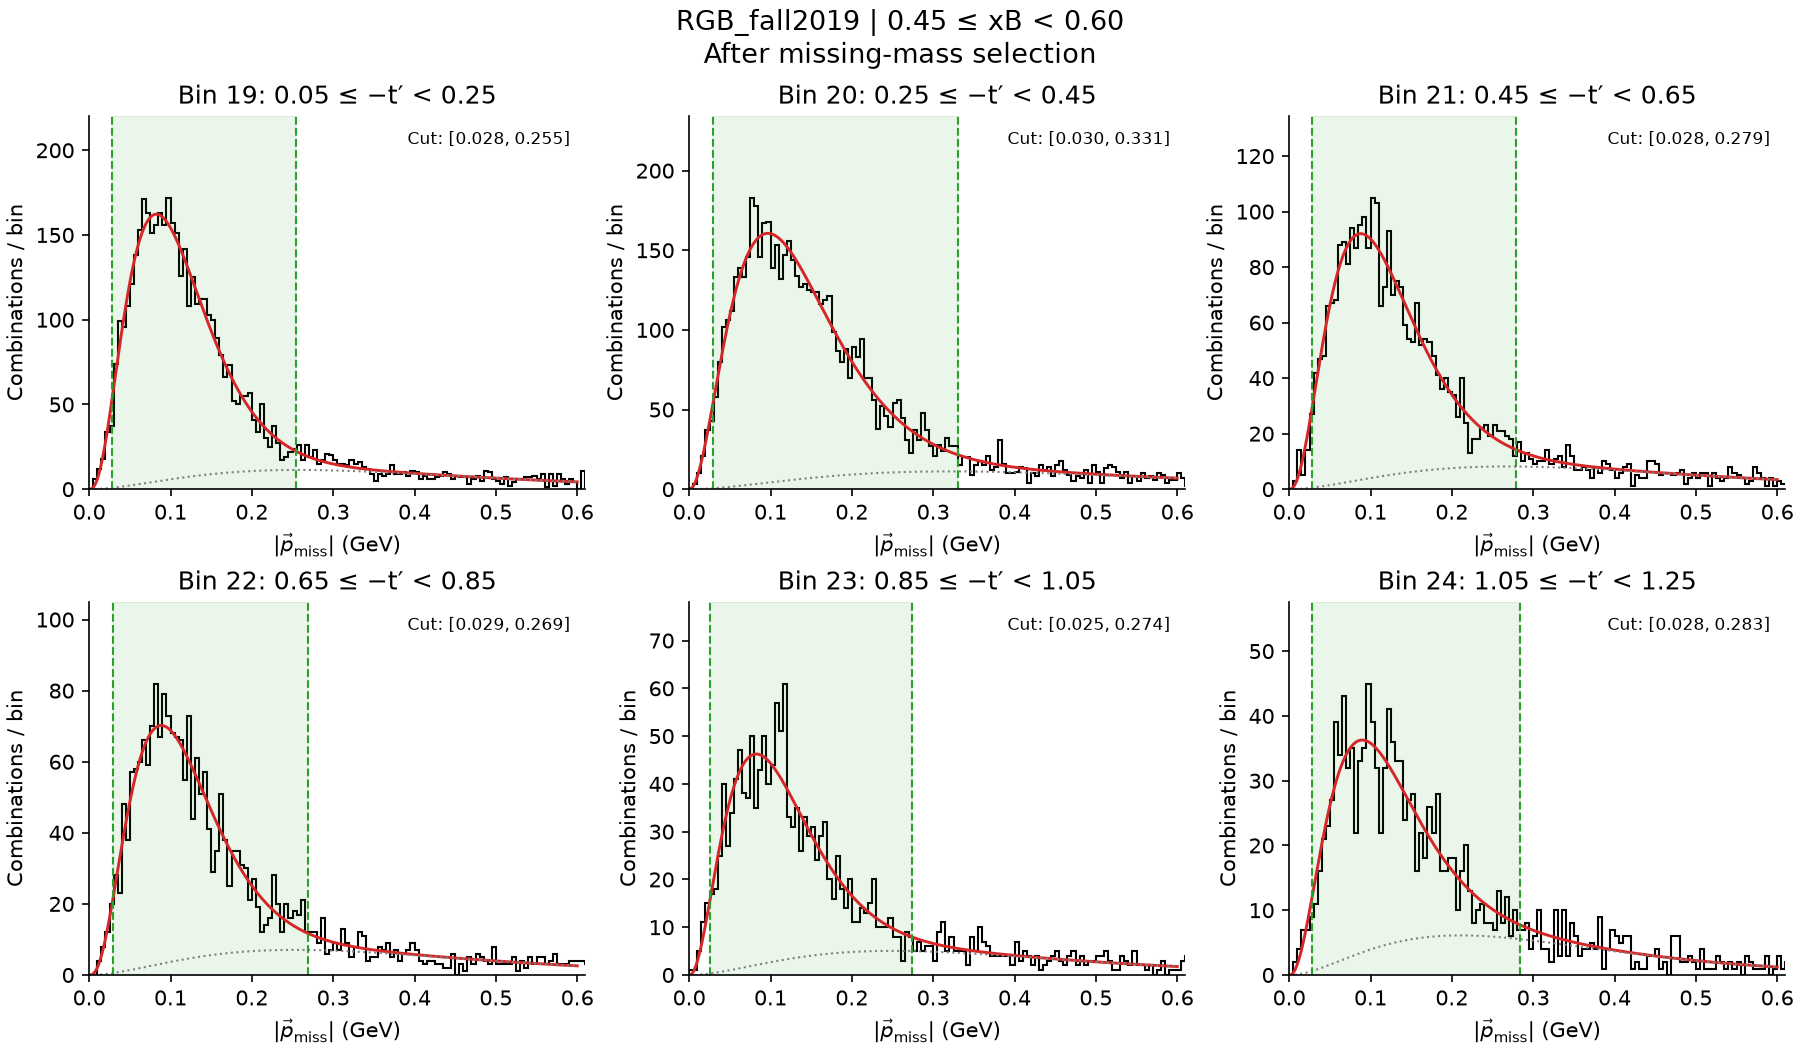
\includegraphics[width=\linewidth]{figures/channel_selection/exclusivity/rgb_fa19_momentum_xb4.png}
\caption{RGB\_fall2019: missing-momentum fits after the mass cut in $x_B$ interval 4. The panels retain the six fine selection bins.}\label{fig:new_excl_rgb_fa19_momentum4}
\end{figure}
\clearpage
\begin{figure}[p]\centering
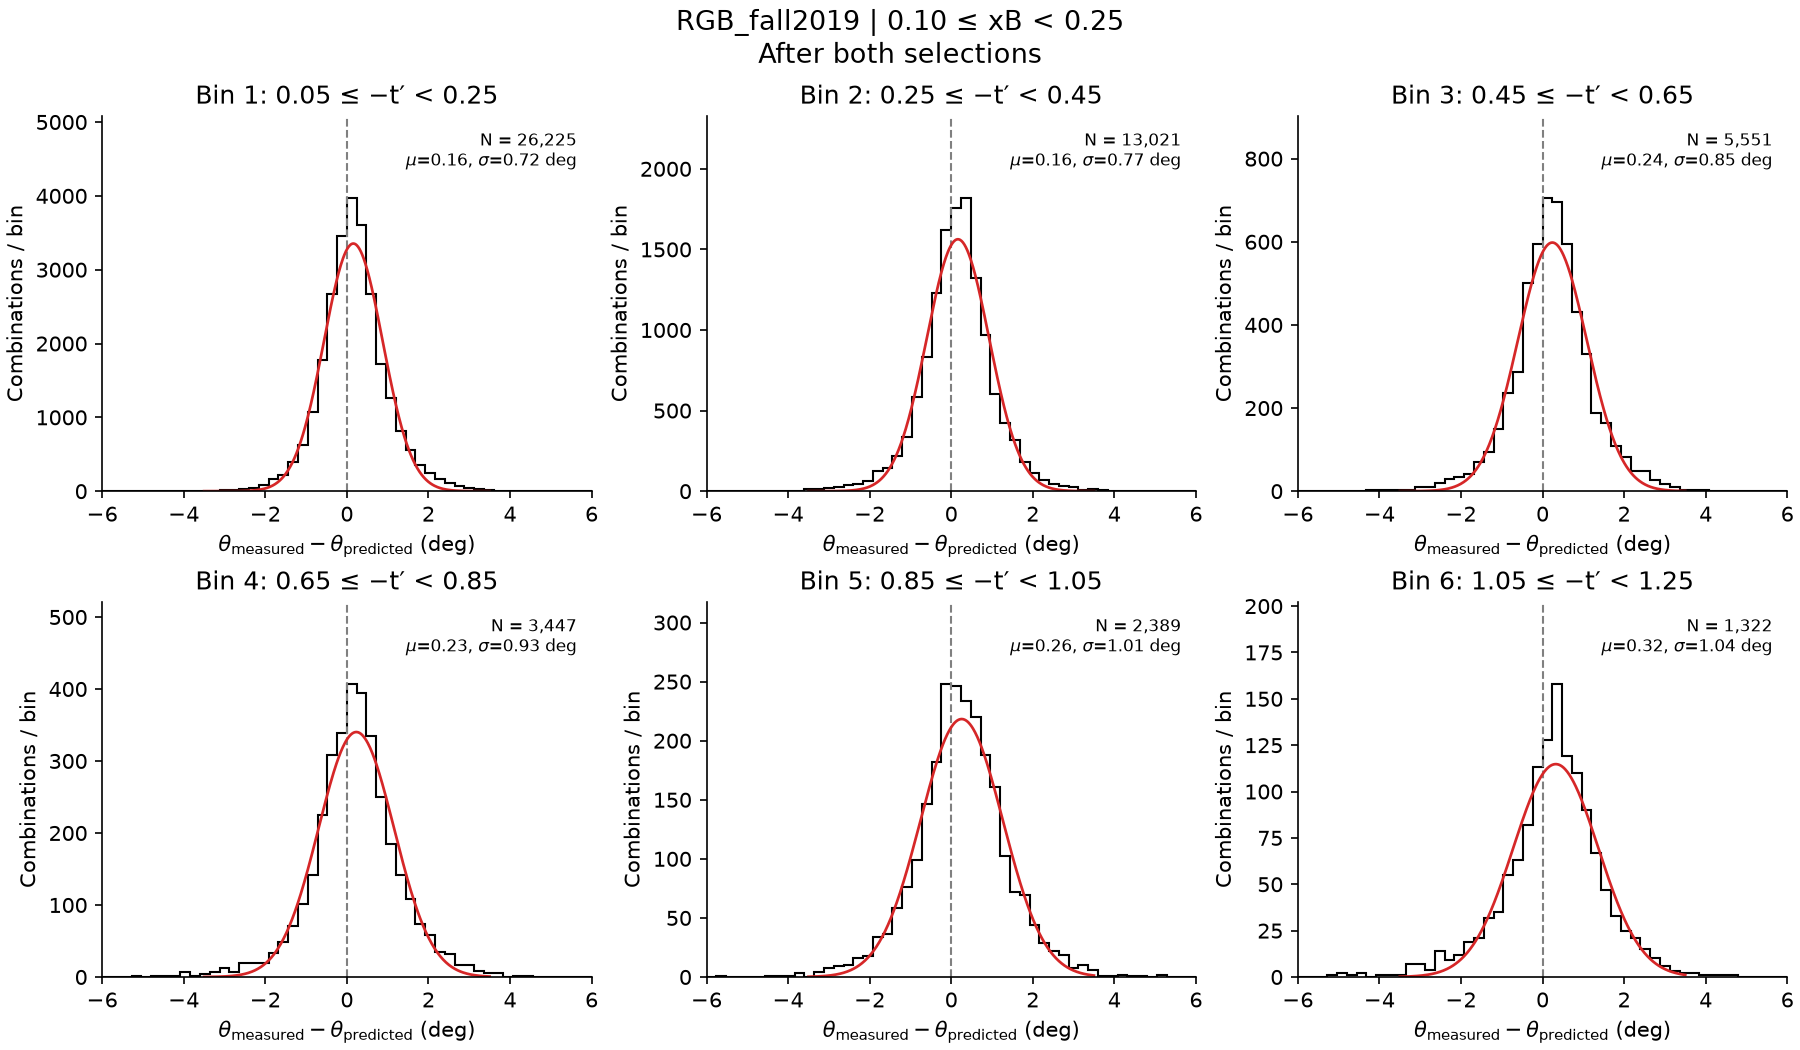
\includegraphics[width=\linewidth]{figures/channel_selection/exclusivity/rgb_fa19_angle_xb1.png}
\caption{RGB\_fall2019: pion polar-angle closure after both cuts in $x_B$ interval 1. The panels retain the six fine selection bins.}\label{fig:new_excl_rgb_fa19_angle1}
\end{figure}
\clearpage
\begin{figure}[p]\centering
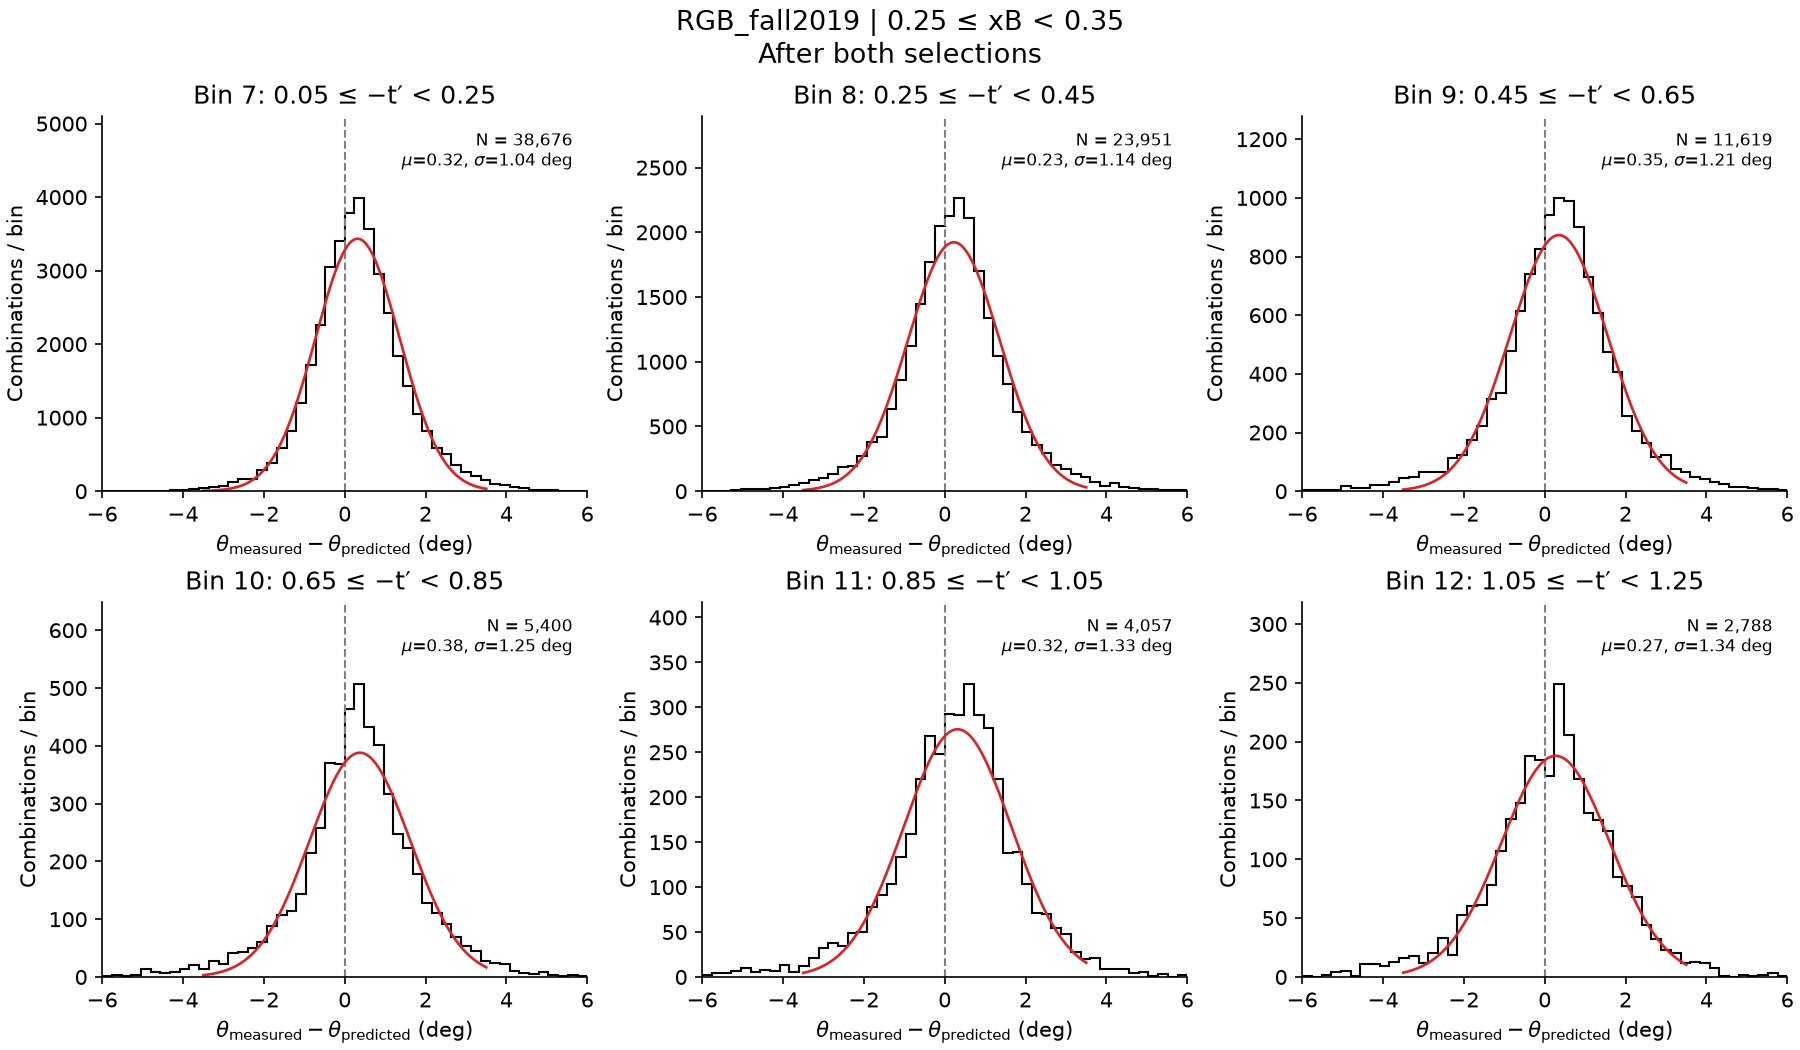
\includegraphics[width=\linewidth]{figures/channel_selection/exclusivity/rgb_fa19_angle_xb2.png}
\caption{RGB\_fall2019: pion polar-angle closure after both cuts in $x_B$ interval 2. The panels retain the six fine selection bins.}\label{fig:new_excl_rgb_fa19_angle2}
\end{figure}
\clearpage
\begin{figure}[p]\centering
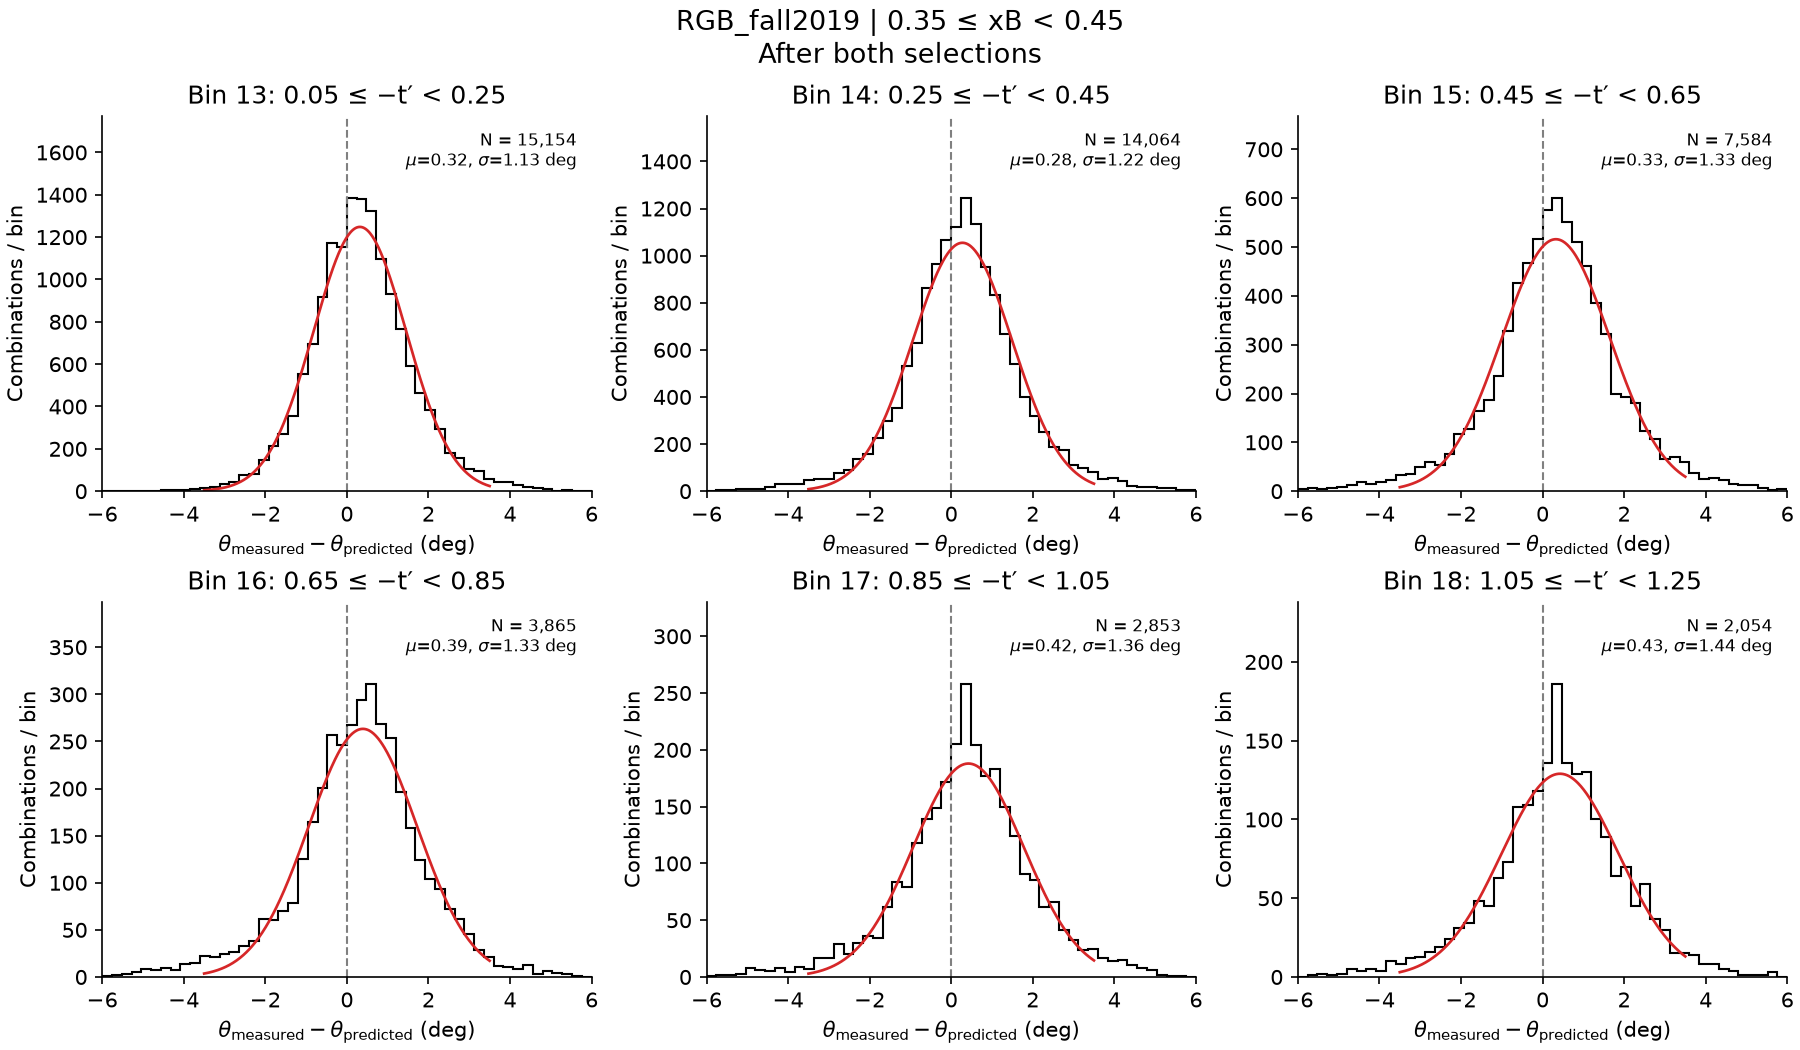
\includegraphics[width=\linewidth]{figures/channel_selection/exclusivity/rgb_fa19_angle_xb3.png}
\caption{RGB\_fall2019: pion polar-angle closure after both cuts in $x_B$ interval 3. The panels retain the six fine selection bins.}\label{fig:new_excl_rgb_fa19_angle3}
\end{figure}
\clearpage
\begin{figure}[p]\centering
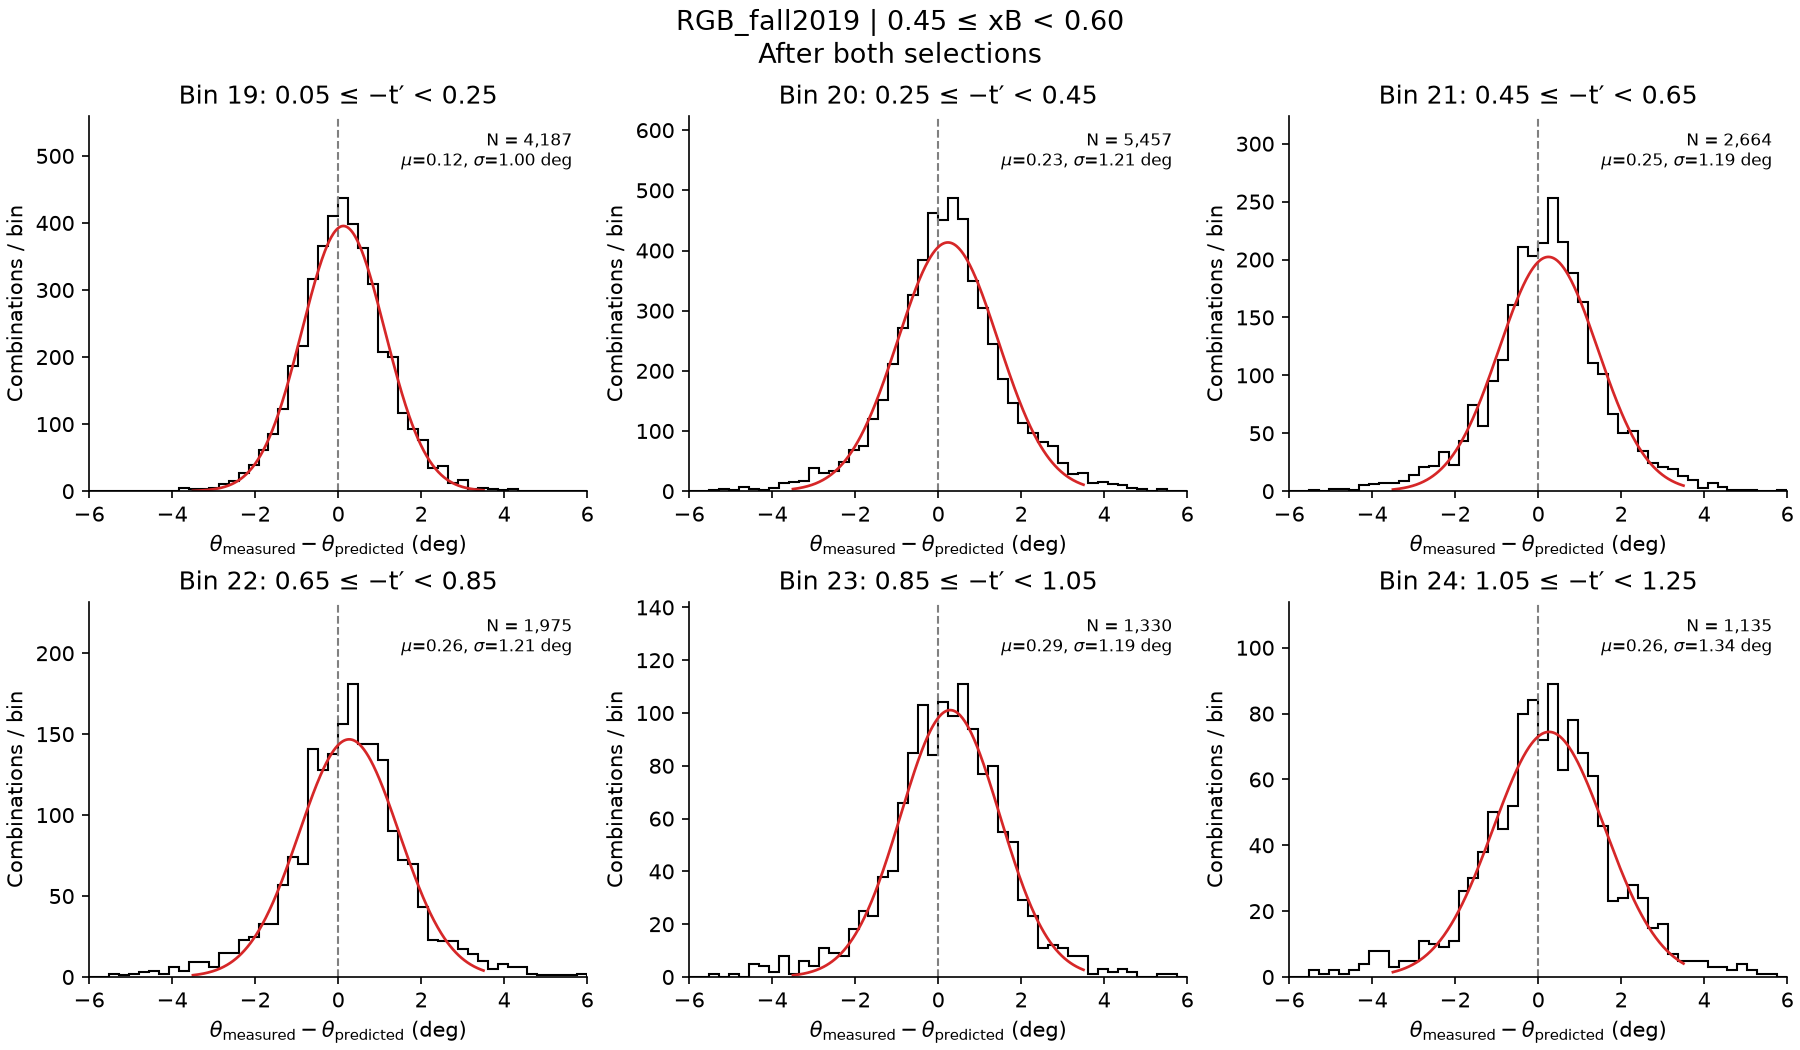
\includegraphics[width=\linewidth]{figures/channel_selection/exclusivity/rgb_fa19_angle_xb4.png}
\caption{RGB\_fall2019: pion polar-angle closure after both cuts in $x_B$ interval 4. The panels retain the six fine selection bins.}\label{fig:new_excl_rgb_fa19_angle4}
\end{figure}
\clearpage
\begin{figure}[p]\centering
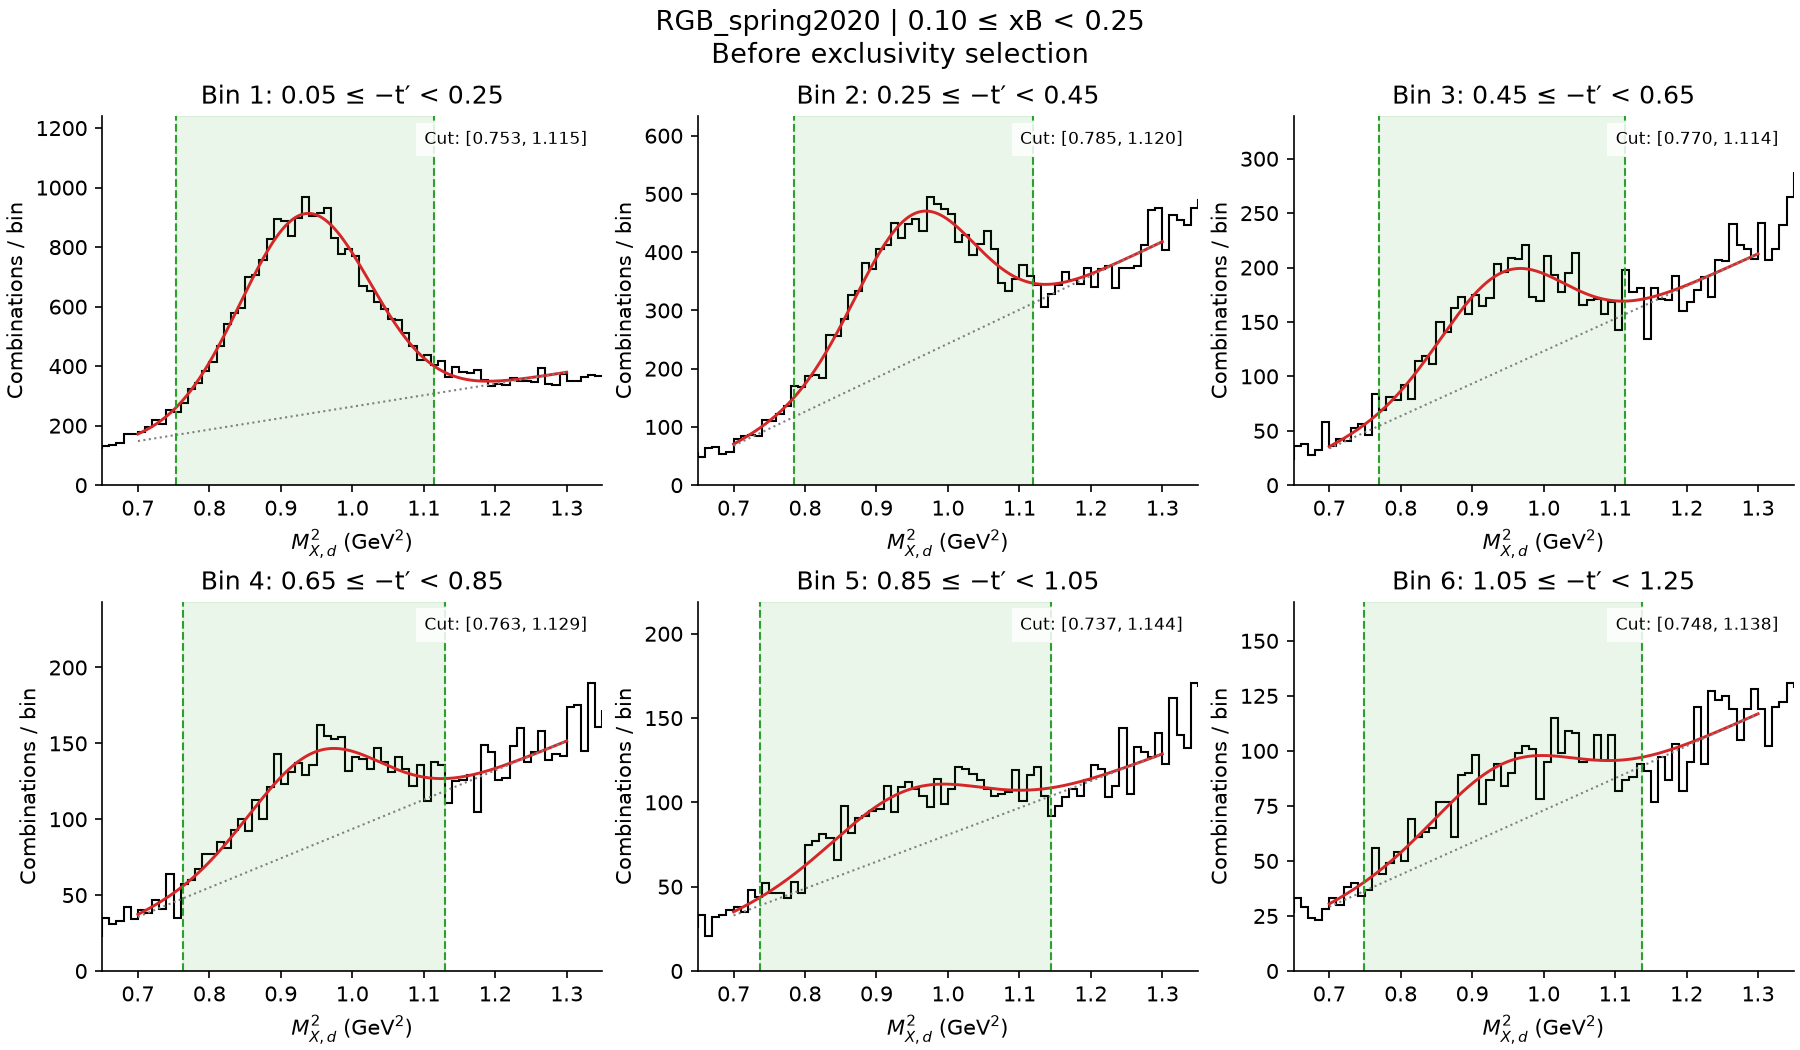
\includegraphics[width=\linewidth]{figures/channel_selection/exclusivity/rgb_sp20_mass_xb1.png}
\caption{RGB\_spring2020: deuteron-reference missing-mass-squared fits in $x_B$ interval 1. The panels retain the six fine selection bins.}\label{fig:new_excl_rgb_sp20_mass1}
\end{figure}
\clearpage
\begin{figure}[p]\centering
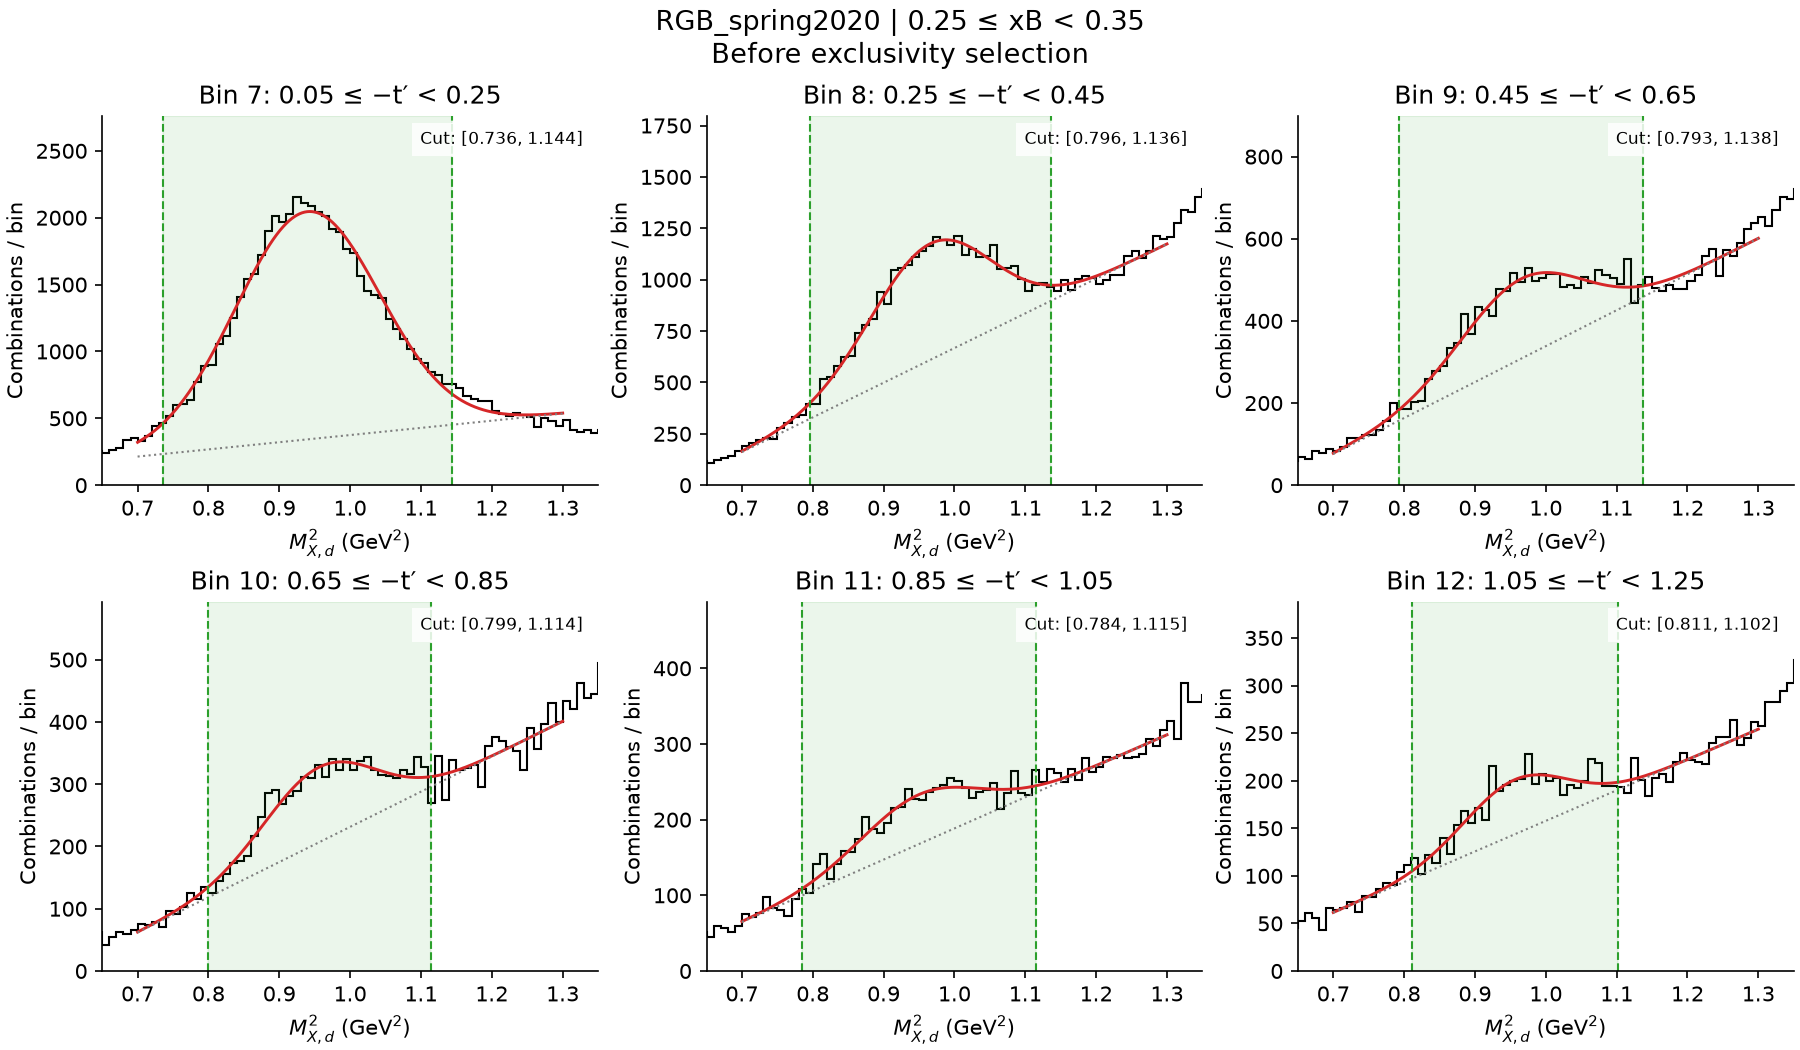
\includegraphics[width=\linewidth]{figures/channel_selection/exclusivity/rgb_sp20_mass_xb2.png}
\caption{RGB\_spring2020: deuteron-reference missing-mass-squared fits in $x_B$ interval 2. The panels retain the six fine selection bins.}\label{fig:new_excl_rgb_sp20_mass2}
\end{figure}
\clearpage
\begin{figure}[p]\centering
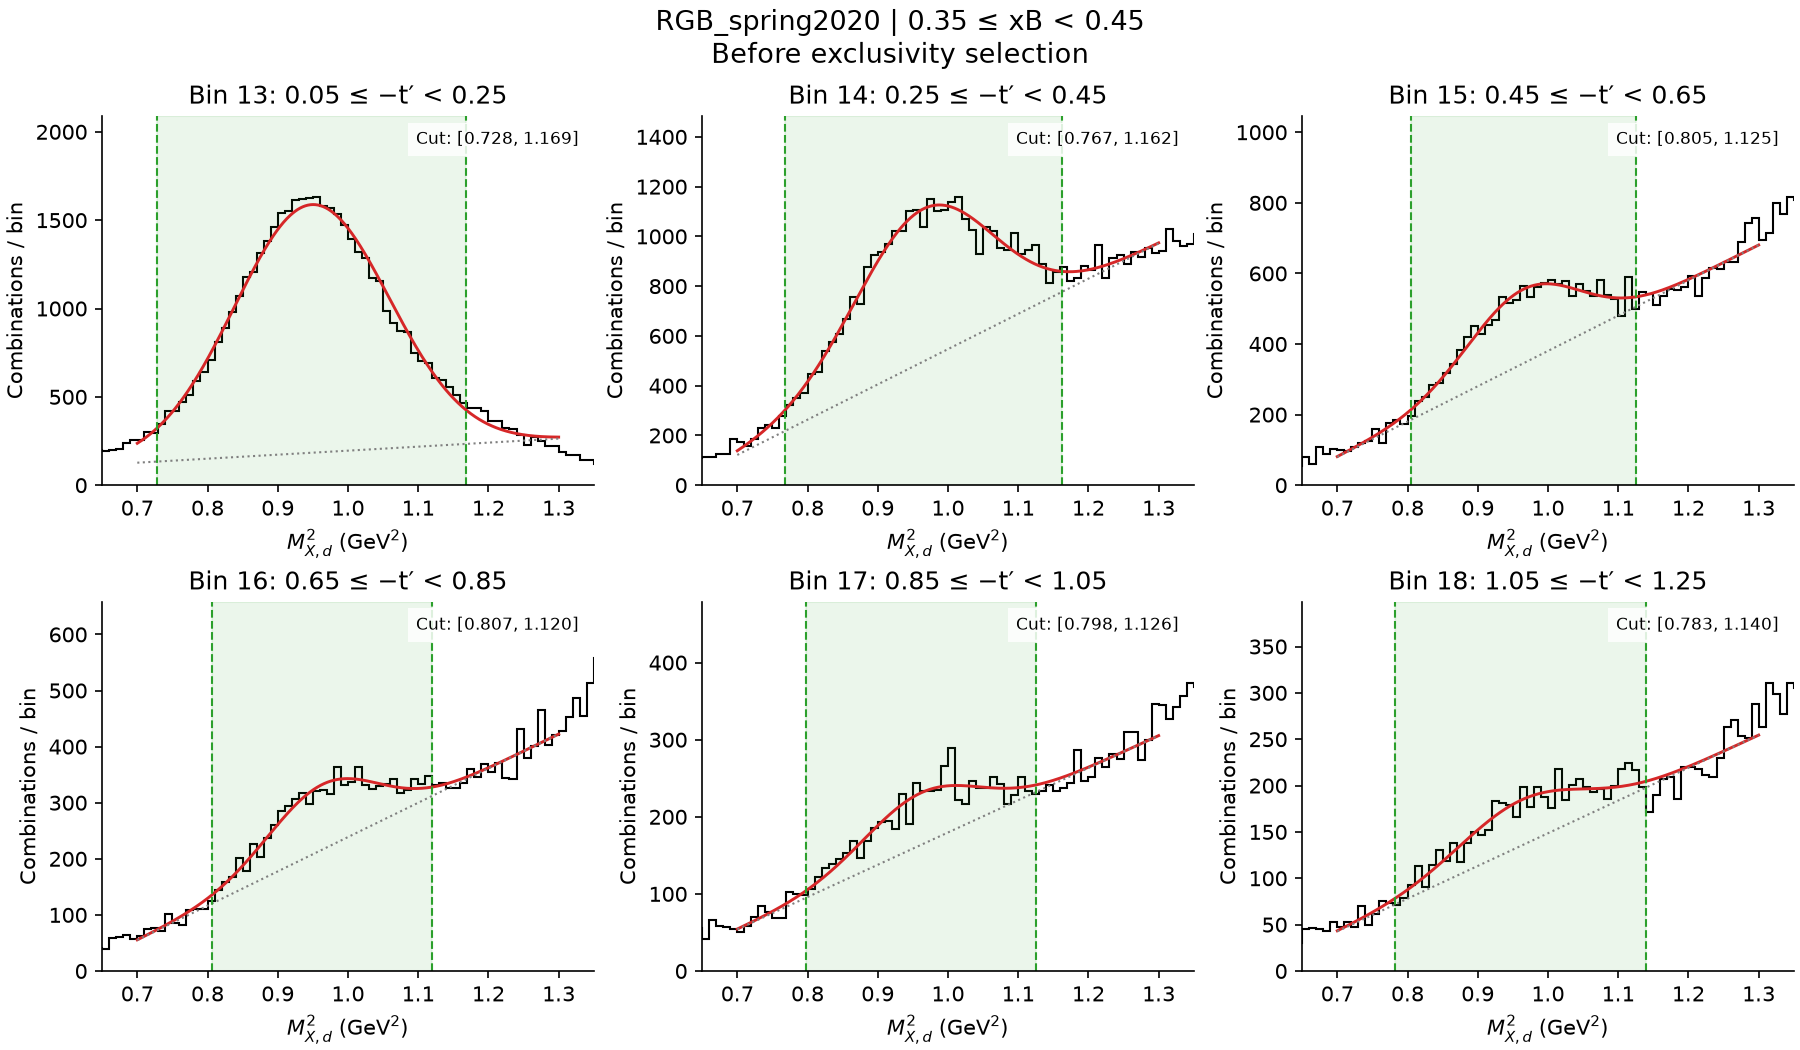
\includegraphics[width=\linewidth]{figures/channel_selection/exclusivity/rgb_sp20_mass_xb3.png}
\caption{RGB\_spring2020: deuteron-reference missing-mass-squared fits in $x_B$ interval 3. The panels retain the six fine selection bins.}\label{fig:new_excl_rgb_sp20_mass3}
\end{figure}
\clearpage
\begin{figure}[p]\centering
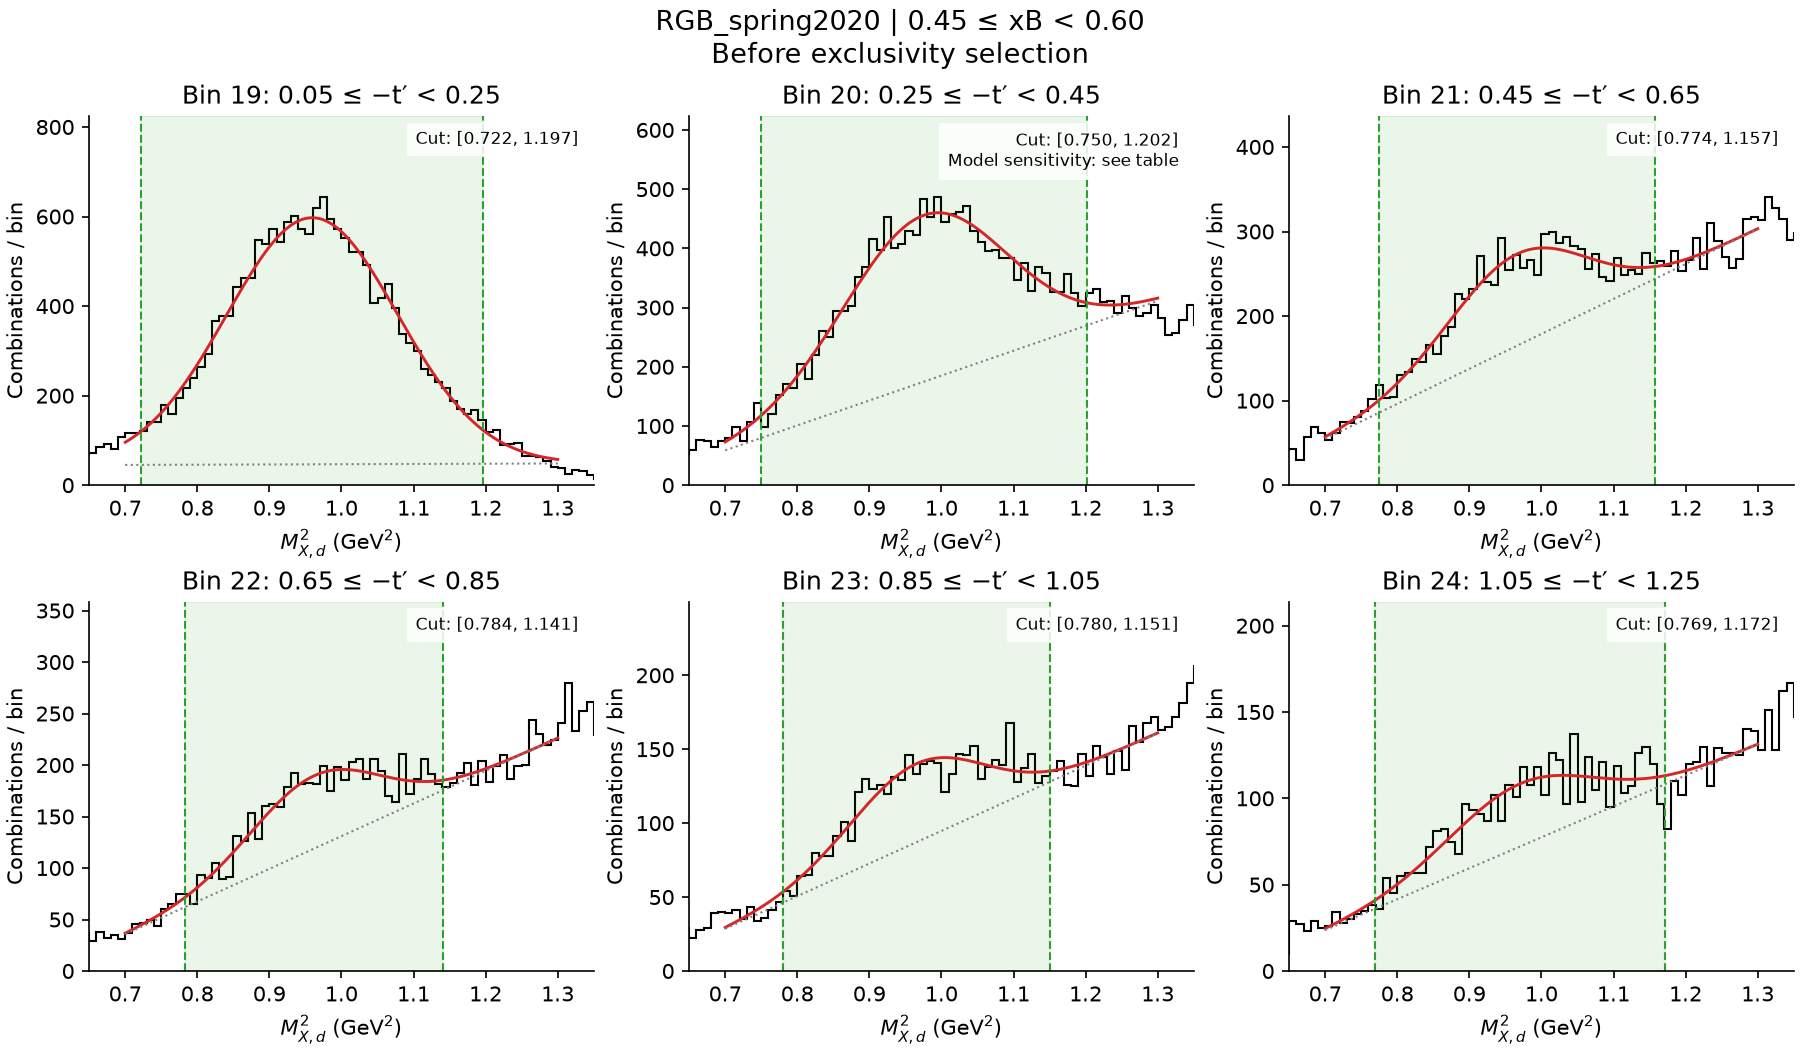
\includegraphics[width=\linewidth]{figures/channel_selection/exclusivity/rgb_sp20_mass_xb4.png}
\caption{RGB\_spring2020: deuteron-reference missing-mass-squared fits in $x_B$ interval 4. The panels retain the six fine selection bins.}\label{fig:new_excl_rgb_sp20_mass4}
\end{figure}
\clearpage
\begin{figure}[p]\centering
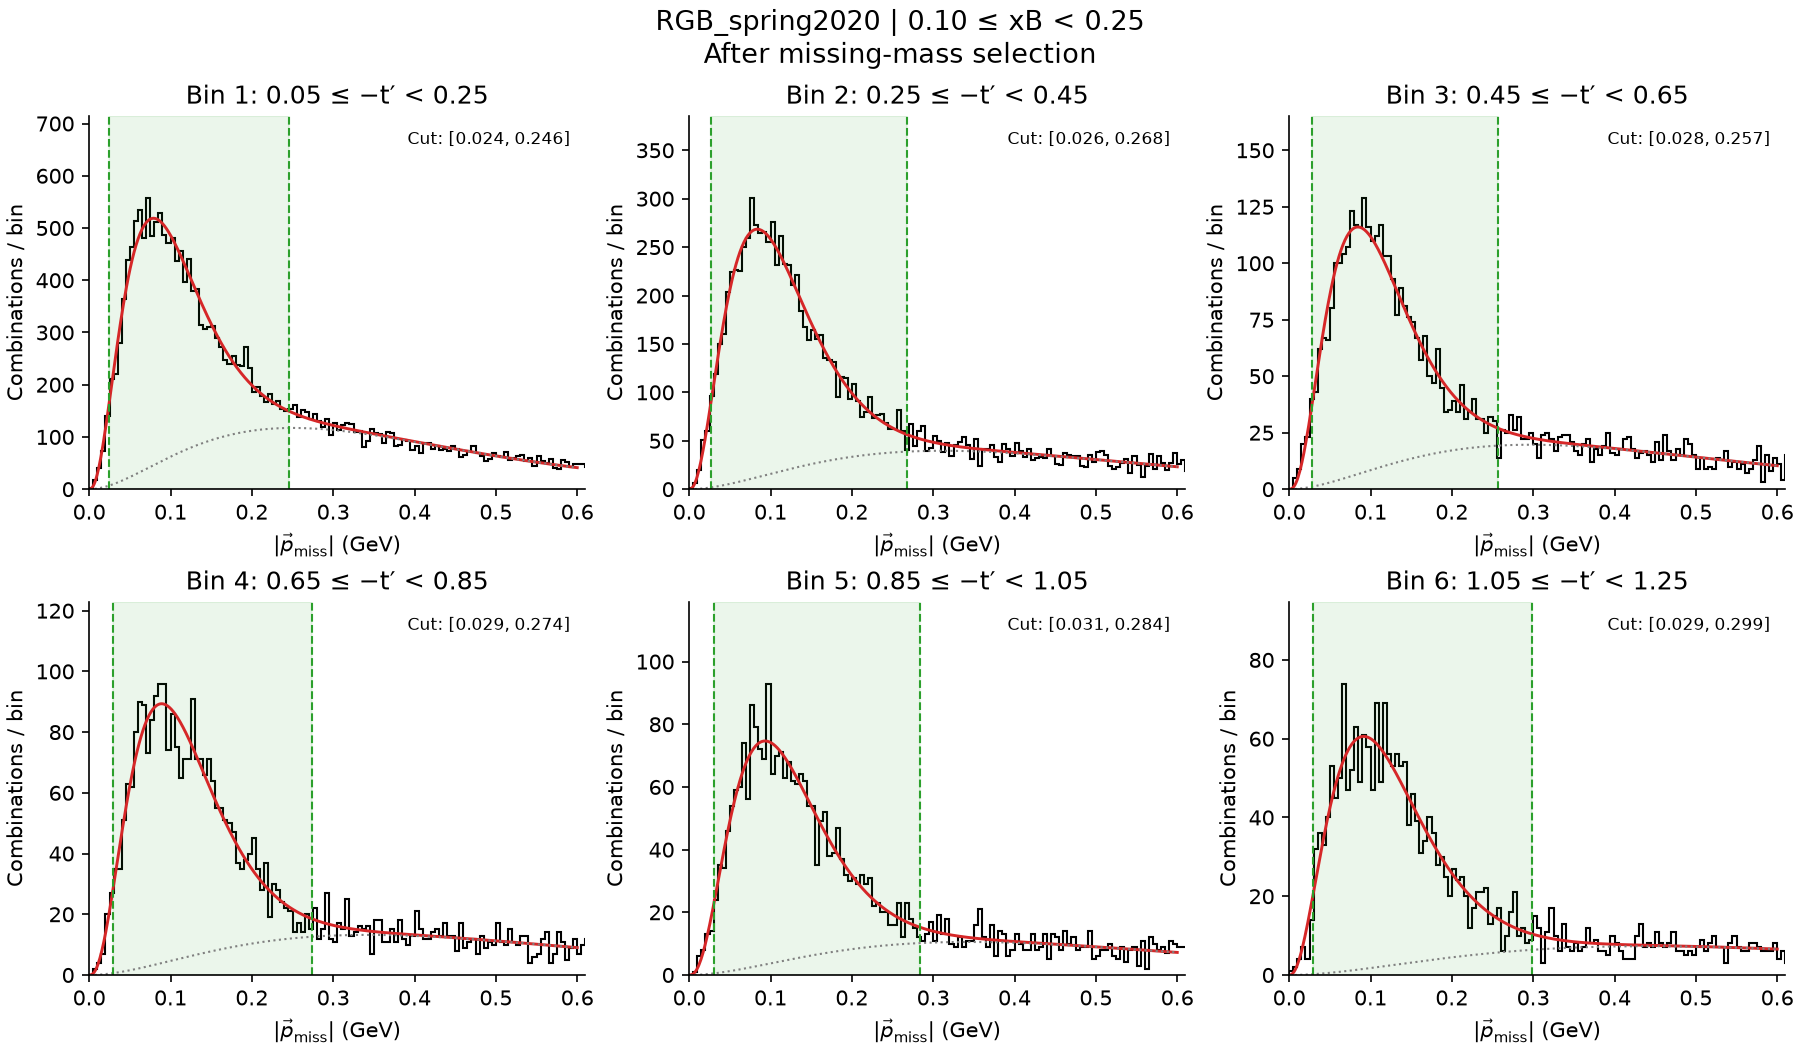
\includegraphics[width=\linewidth]{figures/channel_selection/exclusivity/rgb_sp20_momentum_xb1.png}
\caption{RGB\_spring2020: missing-momentum fits after the mass cut in $x_B$ interval 1. The panels retain the six fine selection bins.}\label{fig:new_excl_rgb_sp20_momentum1}
\end{figure}
\clearpage
\begin{figure}[p]\centering
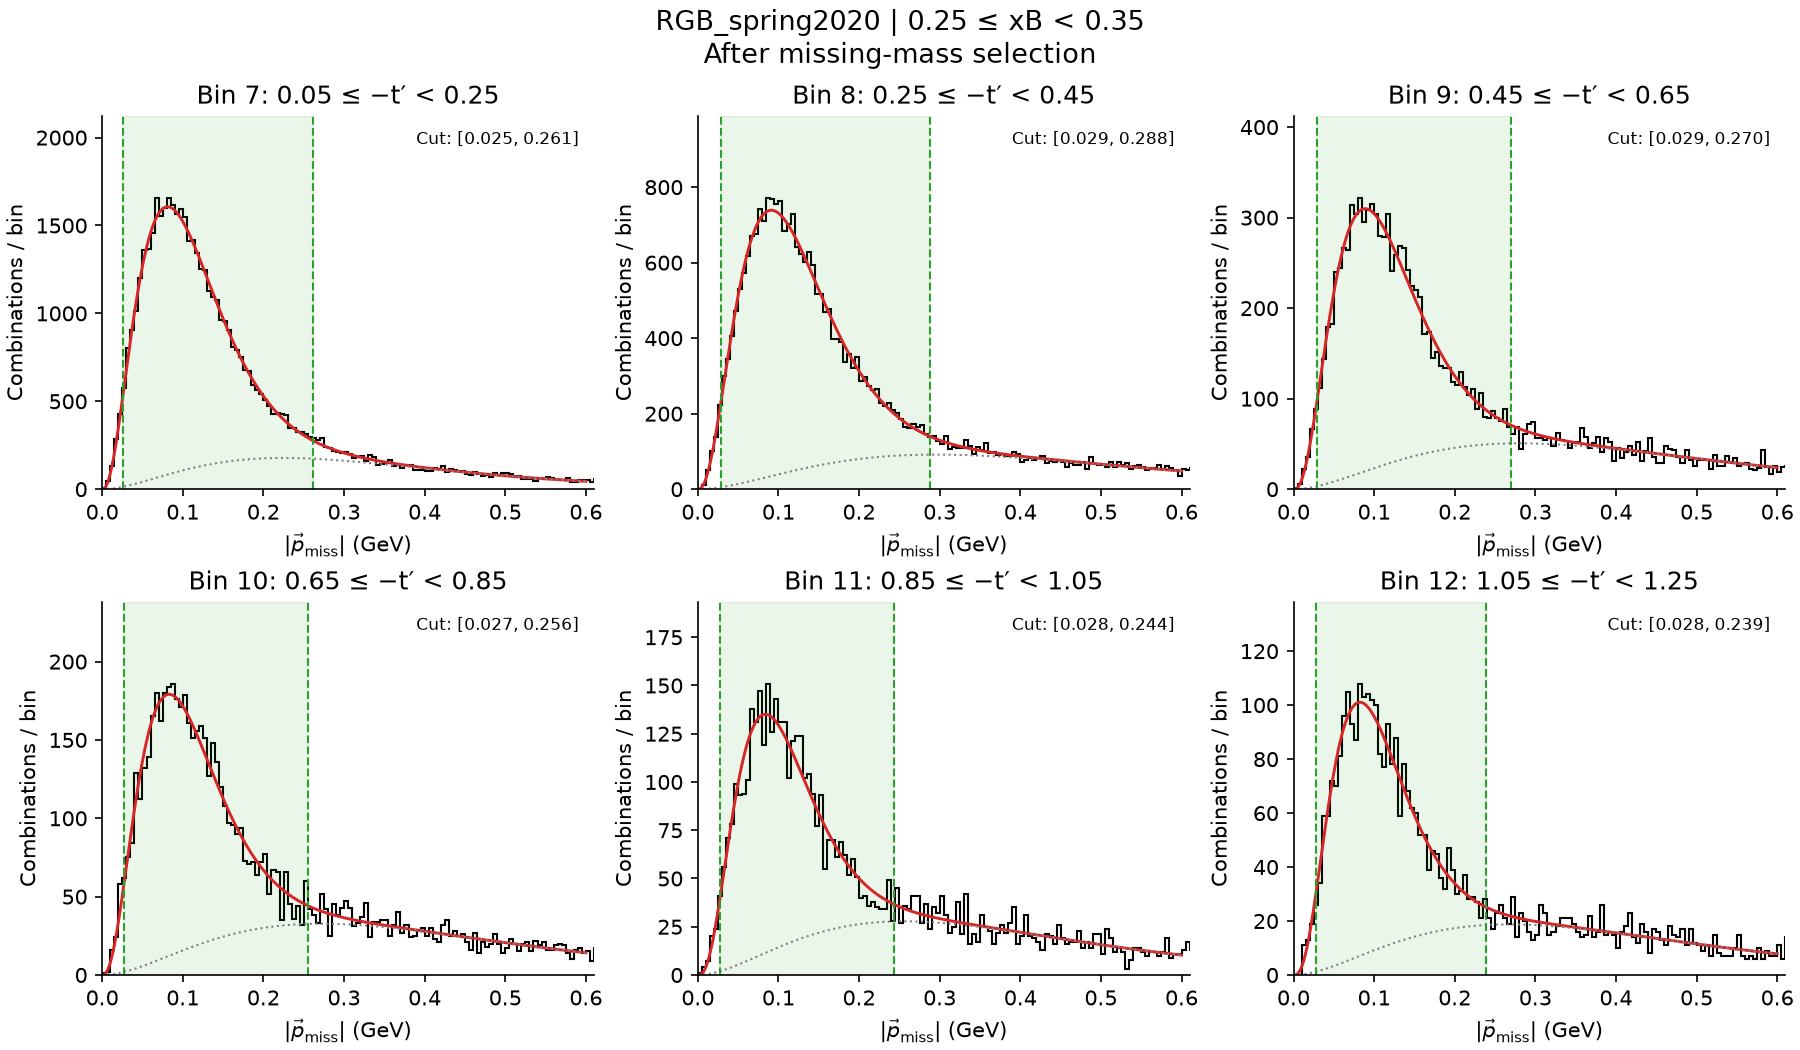
\includegraphics[width=\linewidth]{figures/channel_selection/exclusivity/rgb_sp20_momentum_xb2.png}
\caption{RGB\_spring2020: missing-momentum fits after the mass cut in $x_B$ interval 2. The panels retain the six fine selection bins.}\label{fig:new_excl_rgb_sp20_momentum2}
\end{figure}
\clearpage
\begin{figure}[p]\centering
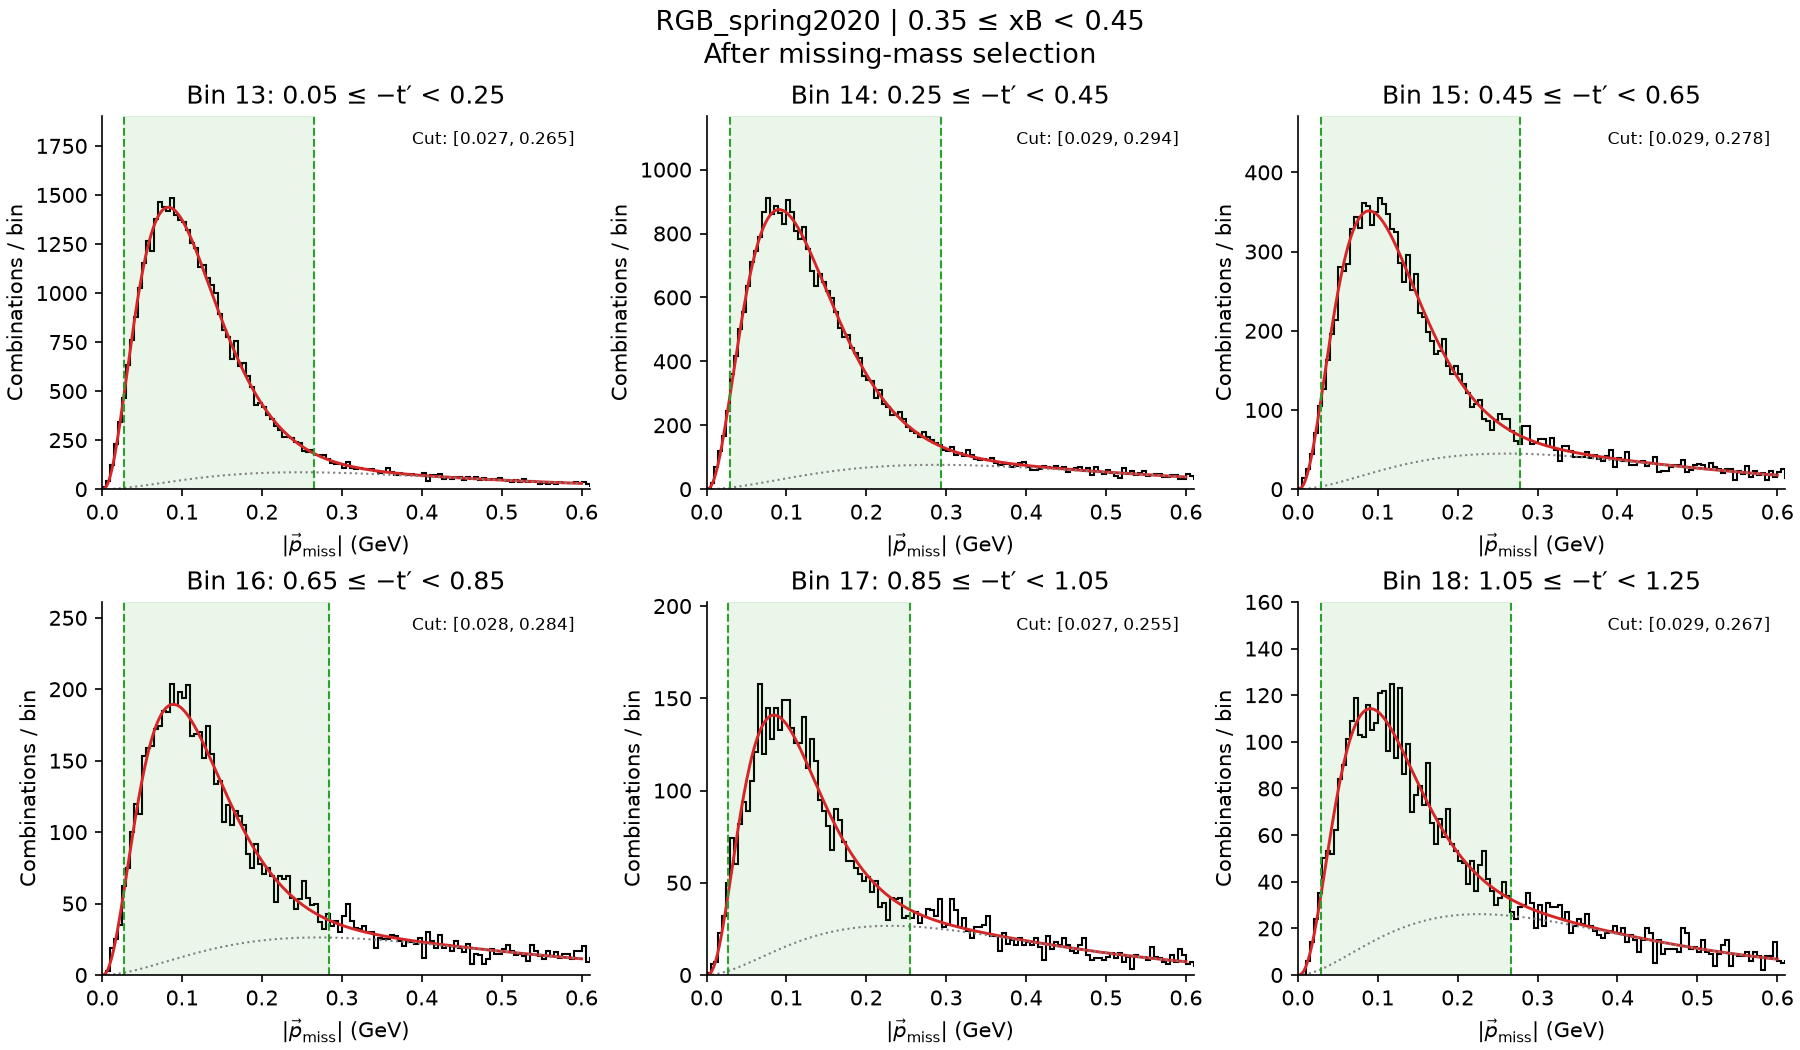
\includegraphics[width=\linewidth]{figures/channel_selection/exclusivity/rgb_sp20_momentum_xb3.png}
\caption{RGB\_spring2020: missing-momentum fits after the mass cut in $x_B$ interval 3. The panels retain the six fine selection bins.}\label{fig:new_excl_rgb_sp20_momentum3}
\end{figure}
\clearpage
\begin{figure}[p]\centering
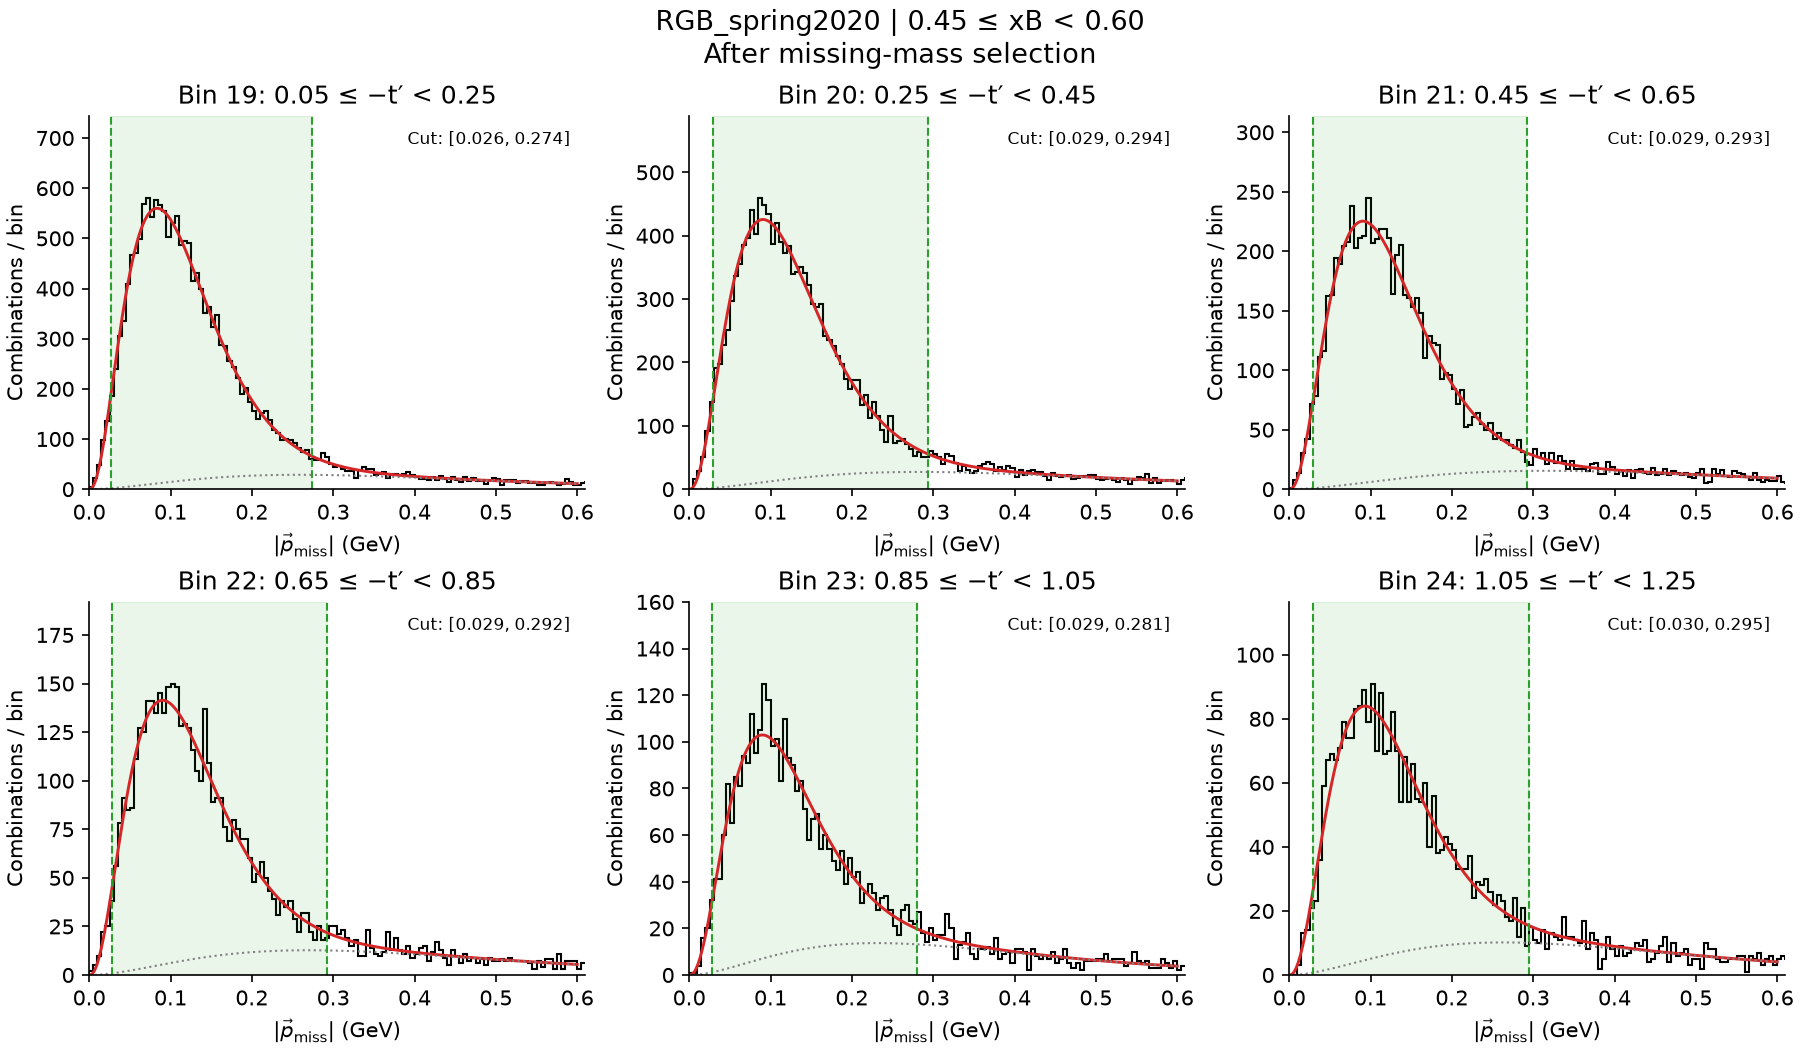
\includegraphics[width=\linewidth]{figures/channel_selection/exclusivity/rgb_sp20_momentum_xb4.png}
\caption{RGB\_spring2020: missing-momentum fits after the mass cut in $x_B$ interval 4. The panels retain the six fine selection bins.}\label{fig:new_excl_rgb_sp20_momentum4}
\end{figure}
\clearpage
\begin{figure}[p]\centering
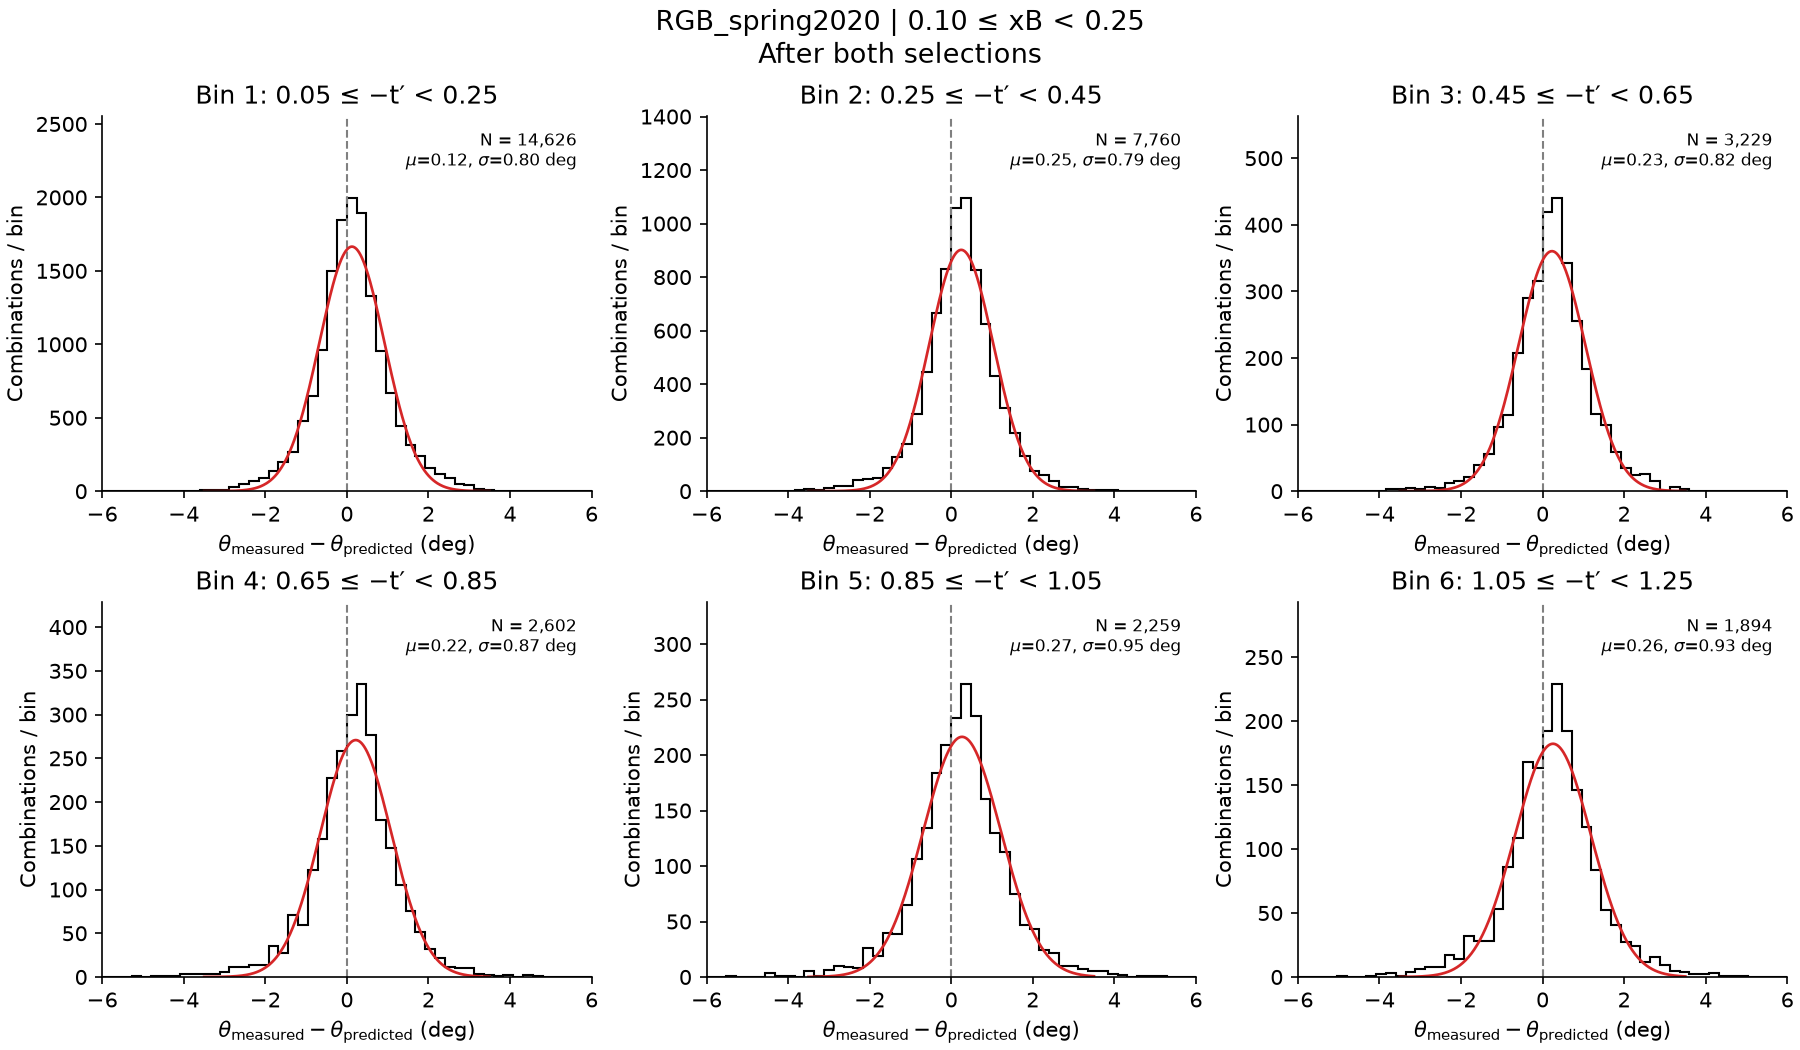
\includegraphics[width=\linewidth]{figures/channel_selection/exclusivity/rgb_sp20_angle_xb1.png}
\caption{RGB\_spring2020: pion polar-angle closure after both cuts in $x_B$ interval 1. The panels retain the six fine selection bins.}\label{fig:new_excl_rgb_sp20_angle1}
\end{figure}
\clearpage
\begin{figure}[p]\centering
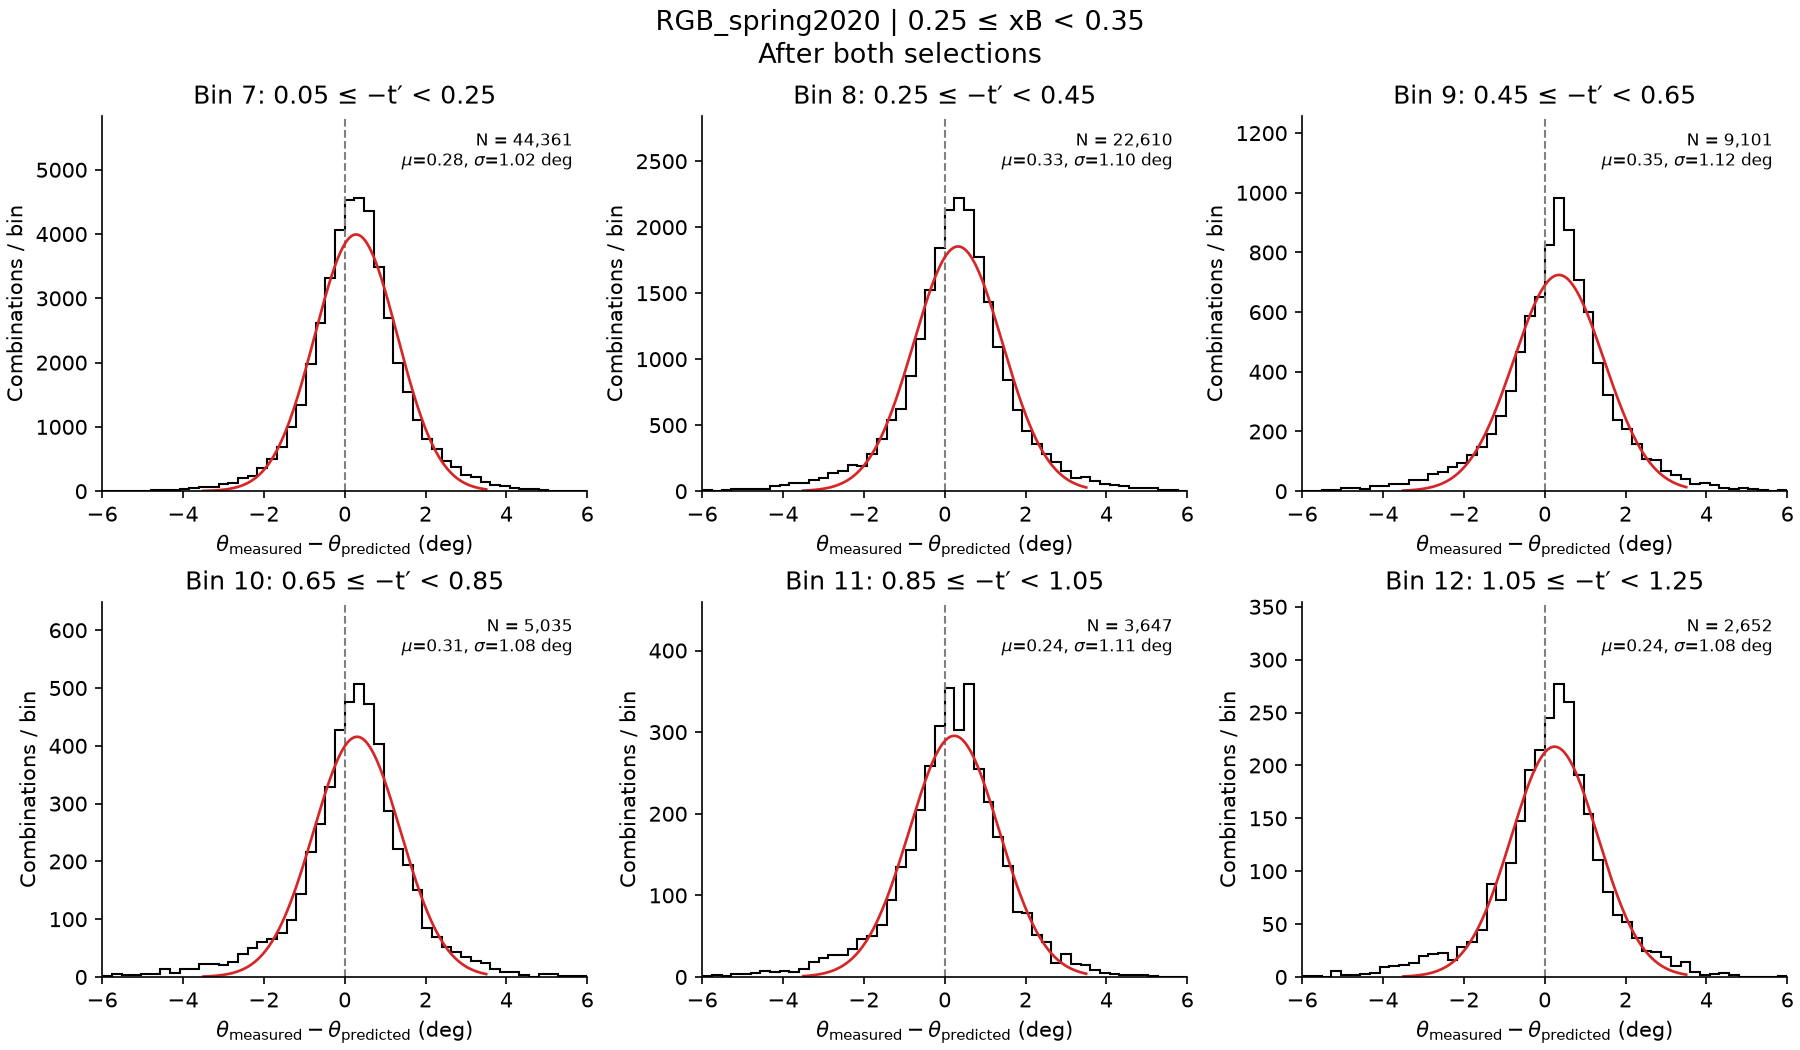
\includegraphics[width=\linewidth]{figures/channel_selection/exclusivity/rgb_sp20_angle_xb2.png}
\caption{RGB\_spring2020: pion polar-angle closure after both cuts in $x_B$ interval 2. The panels retain the six fine selection bins.}\label{fig:new_excl_rgb_sp20_angle2}
\end{figure}
\clearpage
\begin{figure}[p]\centering
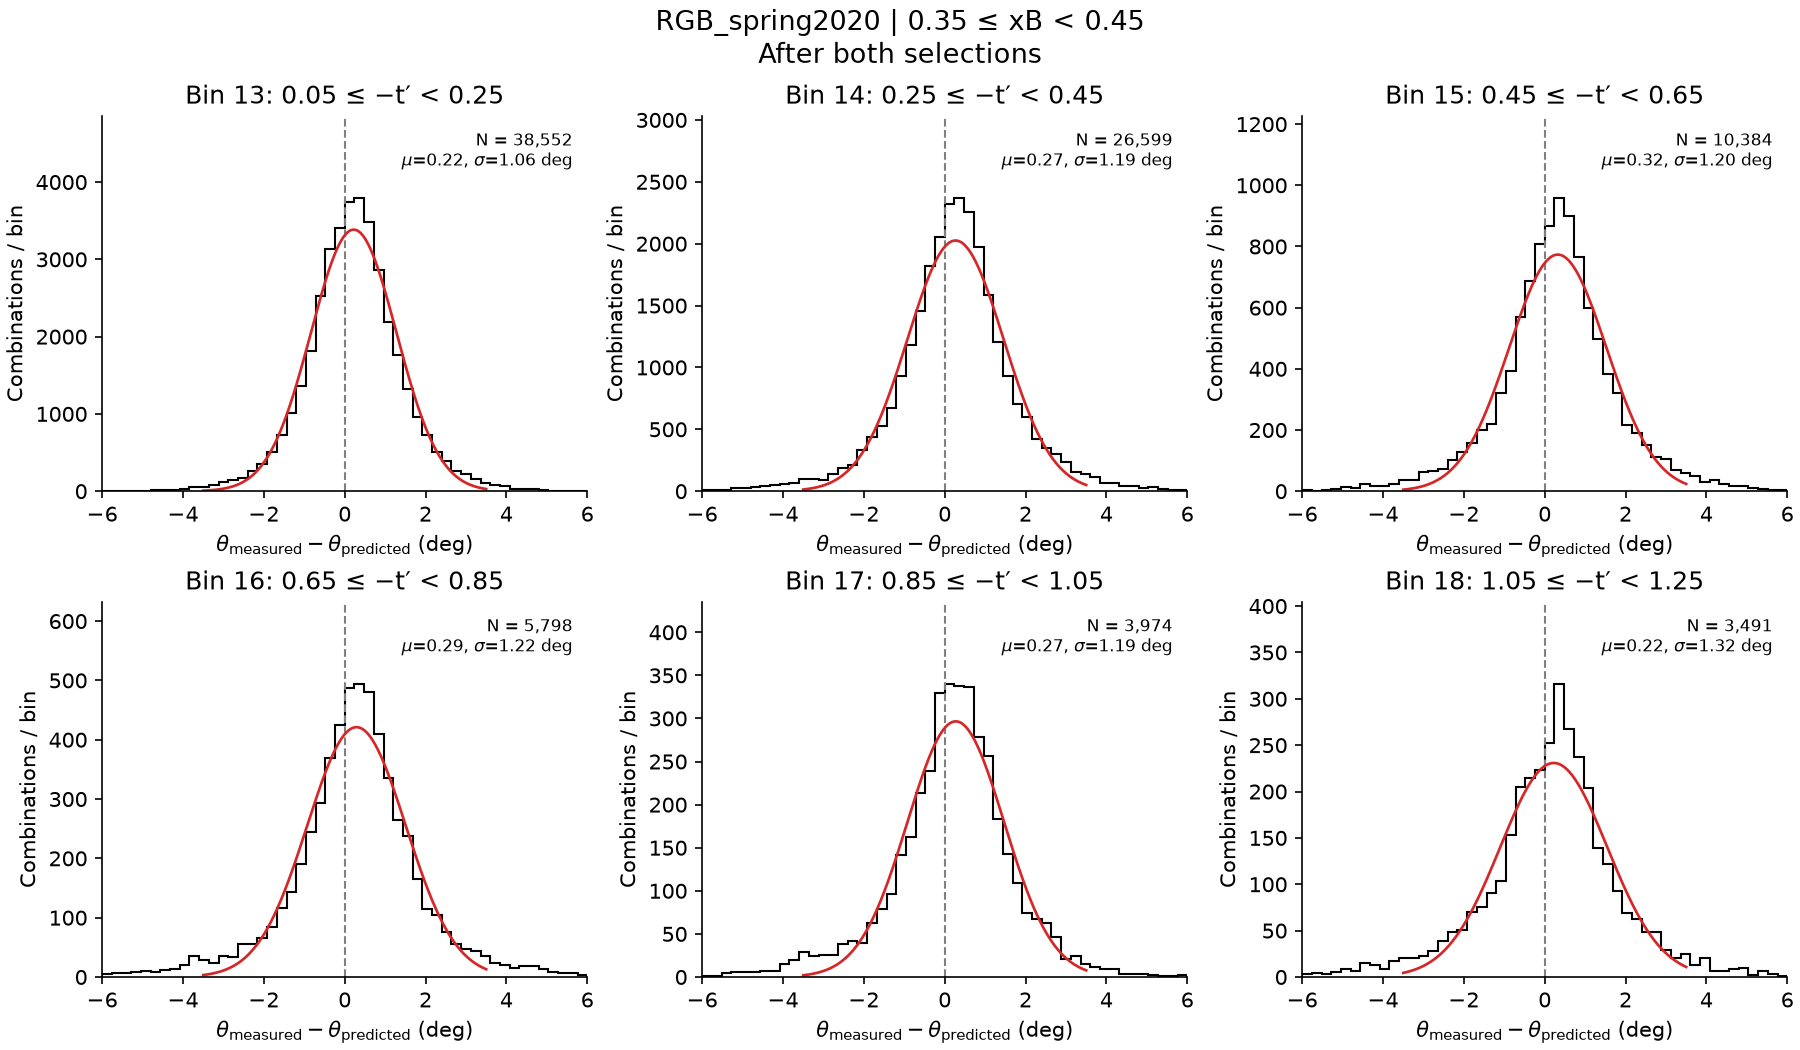
\includegraphics[width=\linewidth]{figures/channel_selection/exclusivity/rgb_sp20_angle_xb3.png}
\caption{RGB\_spring2020: pion polar-angle closure after both cuts in $x_B$ interval 3. The panels retain the six fine selection bins.}\label{fig:new_excl_rgb_sp20_angle3}
\end{figure}
\clearpage
\begin{figure}[p]\centering
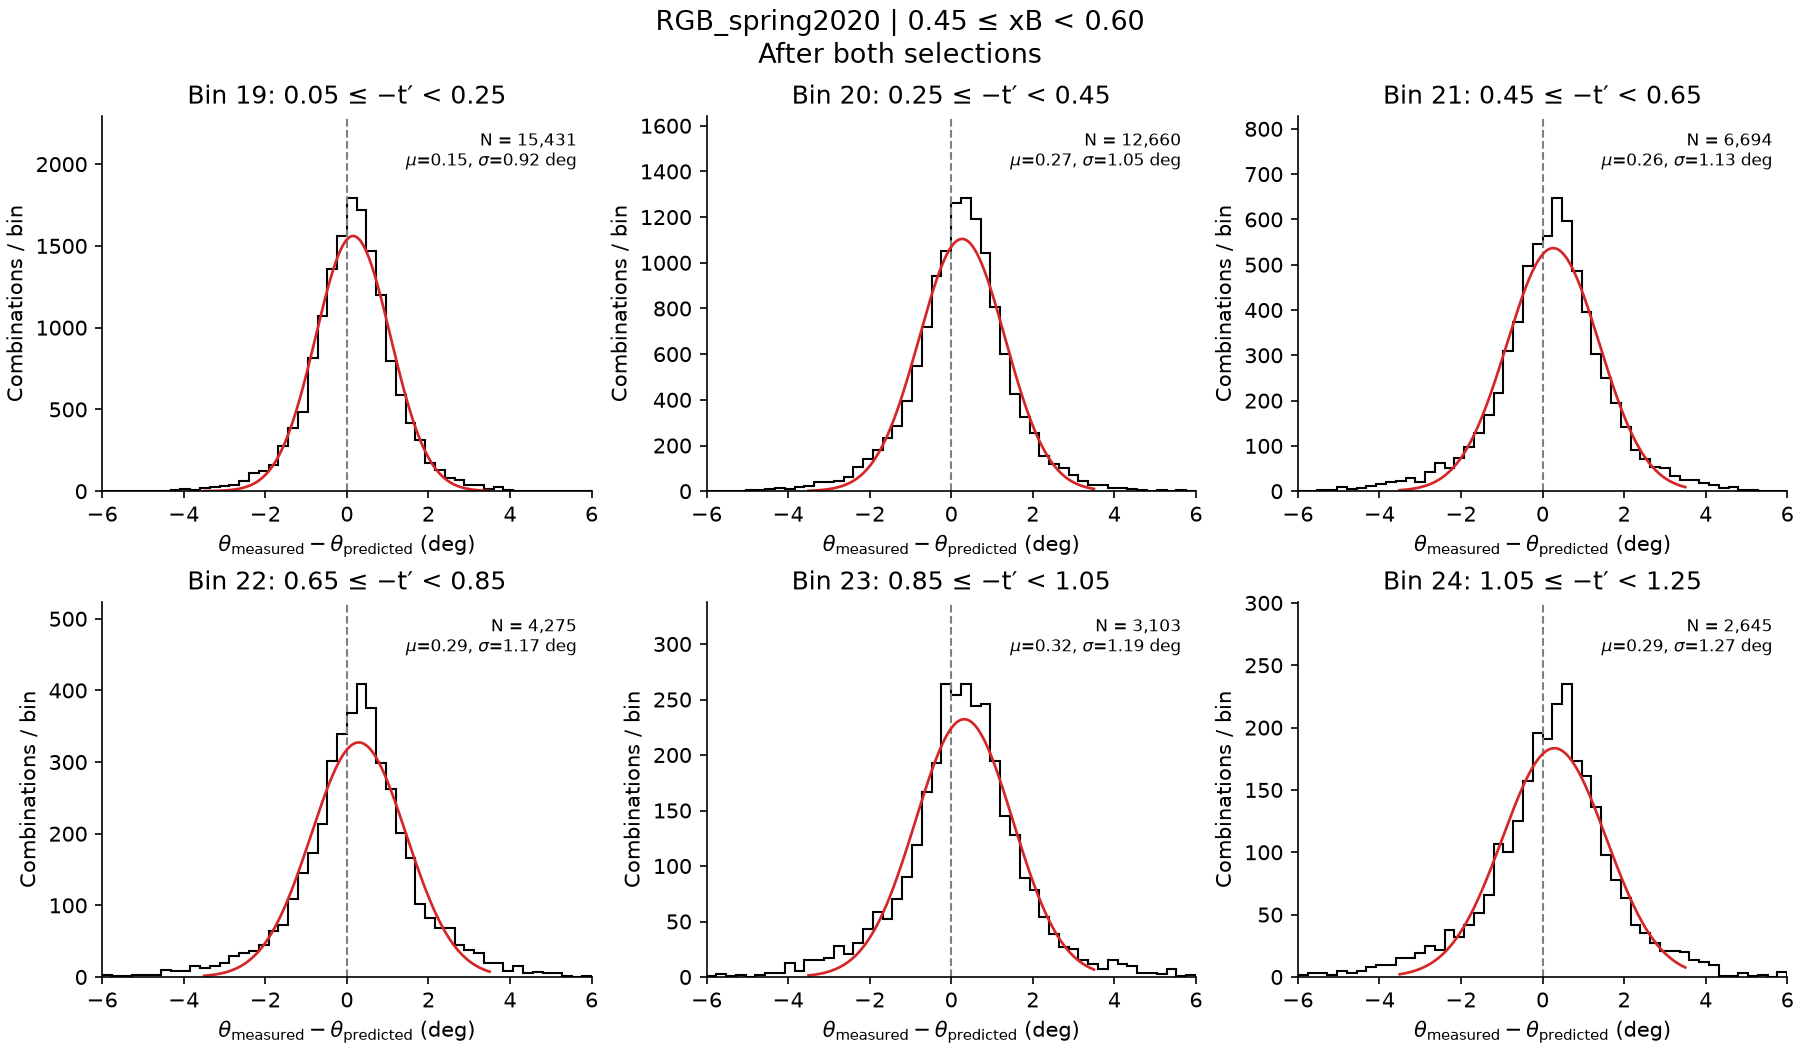
\includegraphics[width=\linewidth]{figures/channel_selection/exclusivity/rgb_sp20_angle_xb4.png}
\caption{RGB\_spring2020: pion polar-angle closure after both cuts in $x_B$ interval 4. The panels retain the six fine selection bins.}\label{fig:new_excl_rgb_sp20_angle4}
\end{figure}
\clearpage
\begin{figure}[p]\centering
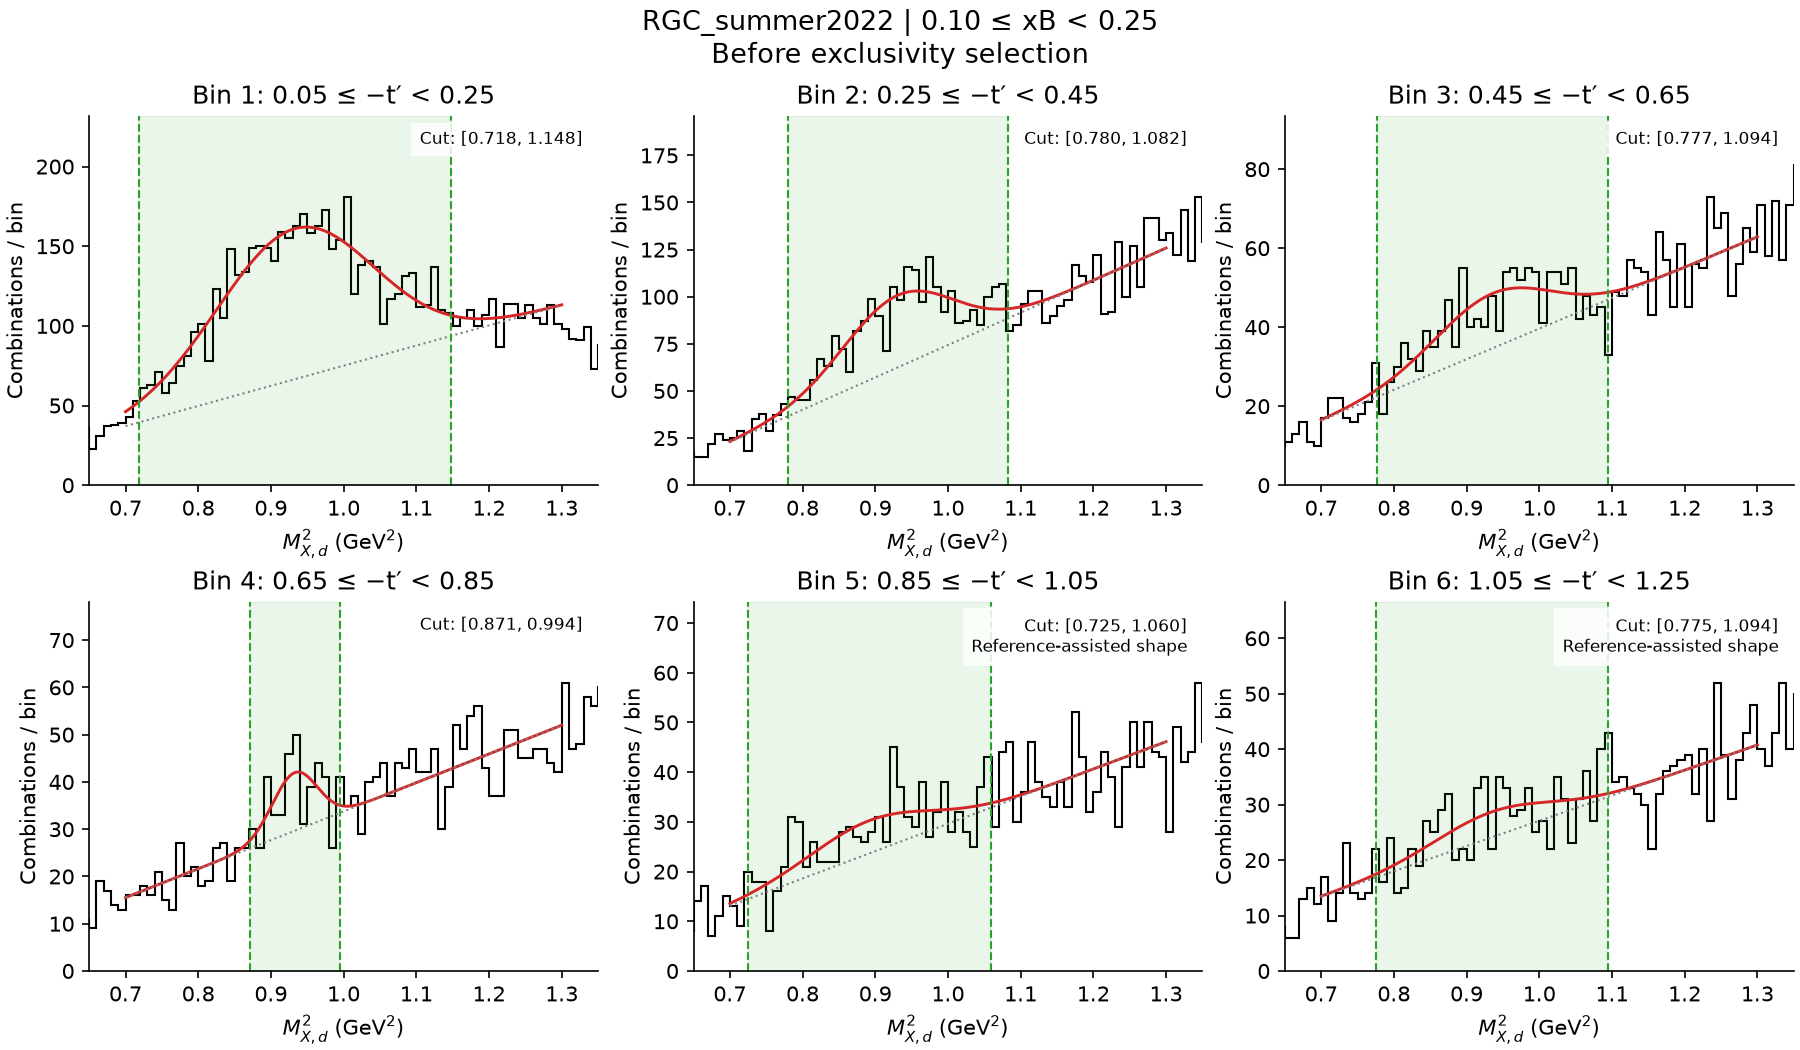
\includegraphics[width=\linewidth]{figures/channel_selection/exclusivity/rgc_su22_mass_xb1.png}
\caption{RGC\_summer2022: deuteron-reference missing-mass-squared fits in $x_B$ interval 1. The panels retain the six fine selection bins.}\label{fig:new_excl_rgc_su22_mass1}
\end{figure}
\clearpage
\begin{figure}[p]\centering
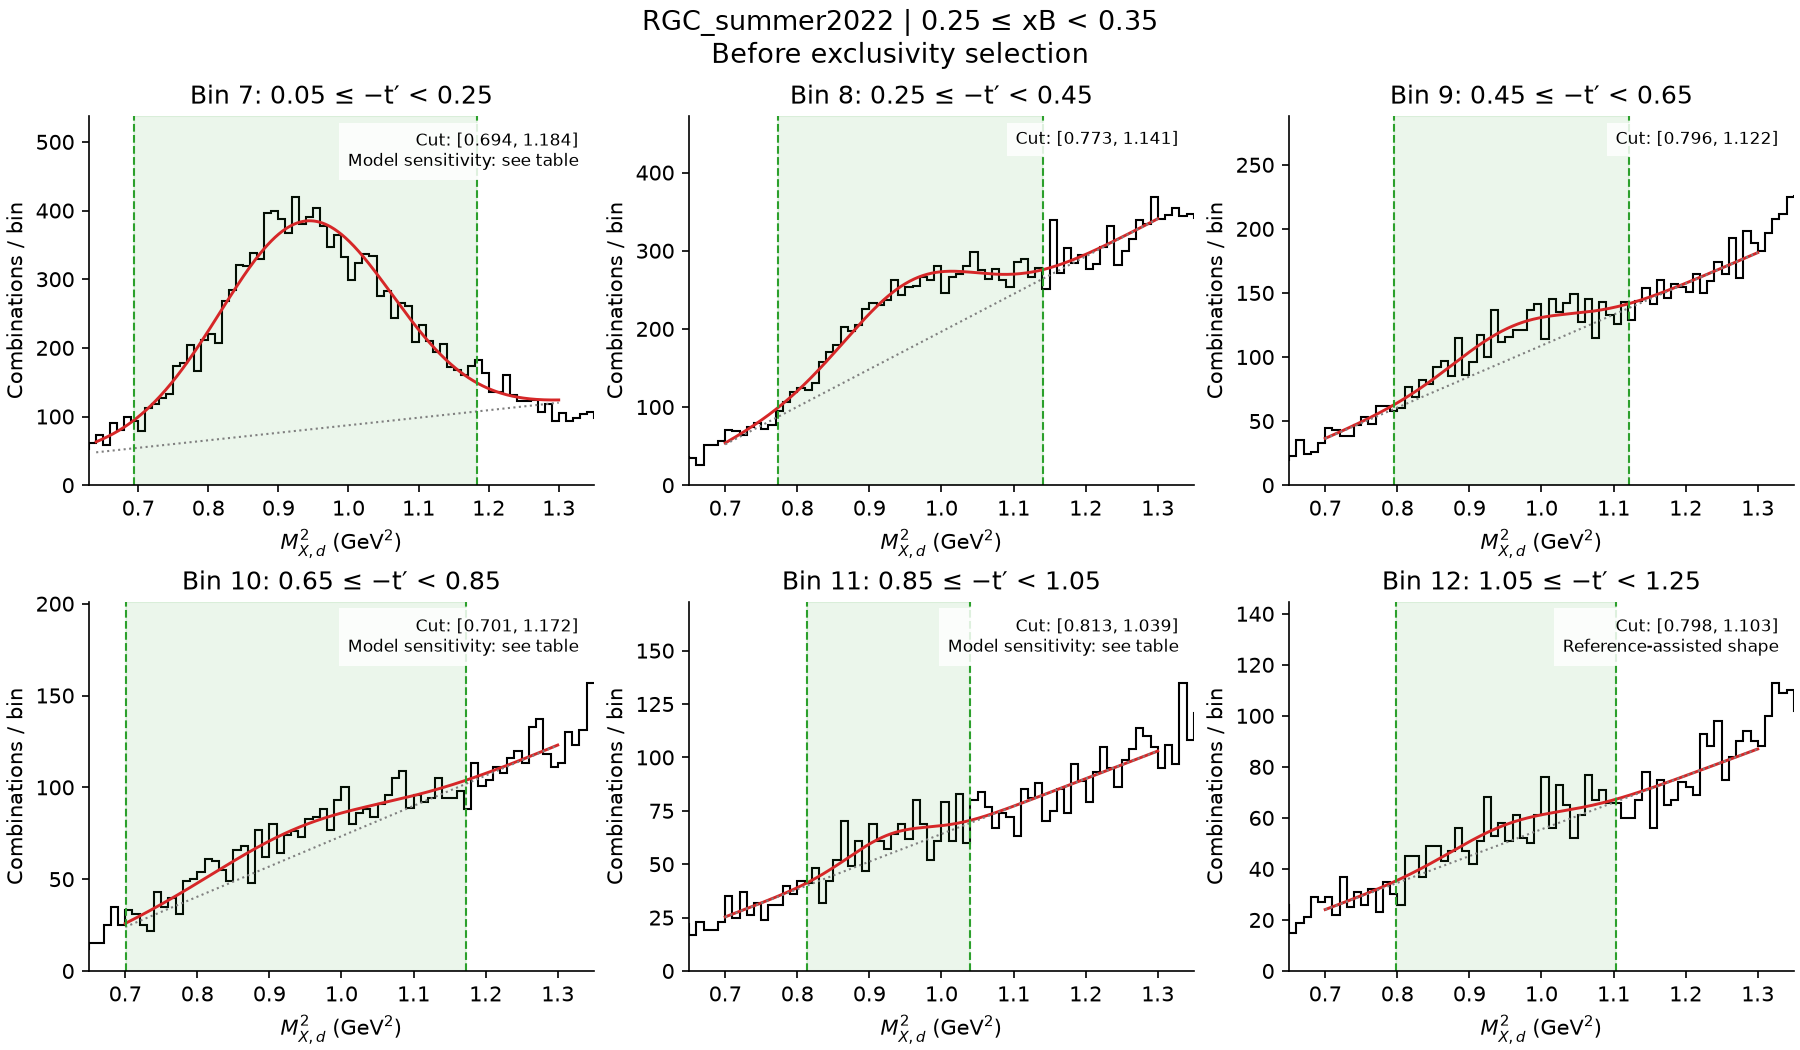
\includegraphics[width=\linewidth]{figures/channel_selection/exclusivity/rgc_su22_mass_xb2.png}
\caption{RGC\_summer2022: deuteron-reference missing-mass-squared fits in $x_B$ interval 2. The panels retain the six fine selection bins.}\label{fig:new_excl_rgc_su22_mass2}
\end{figure}
\clearpage
\begin{figure}[p]\centering
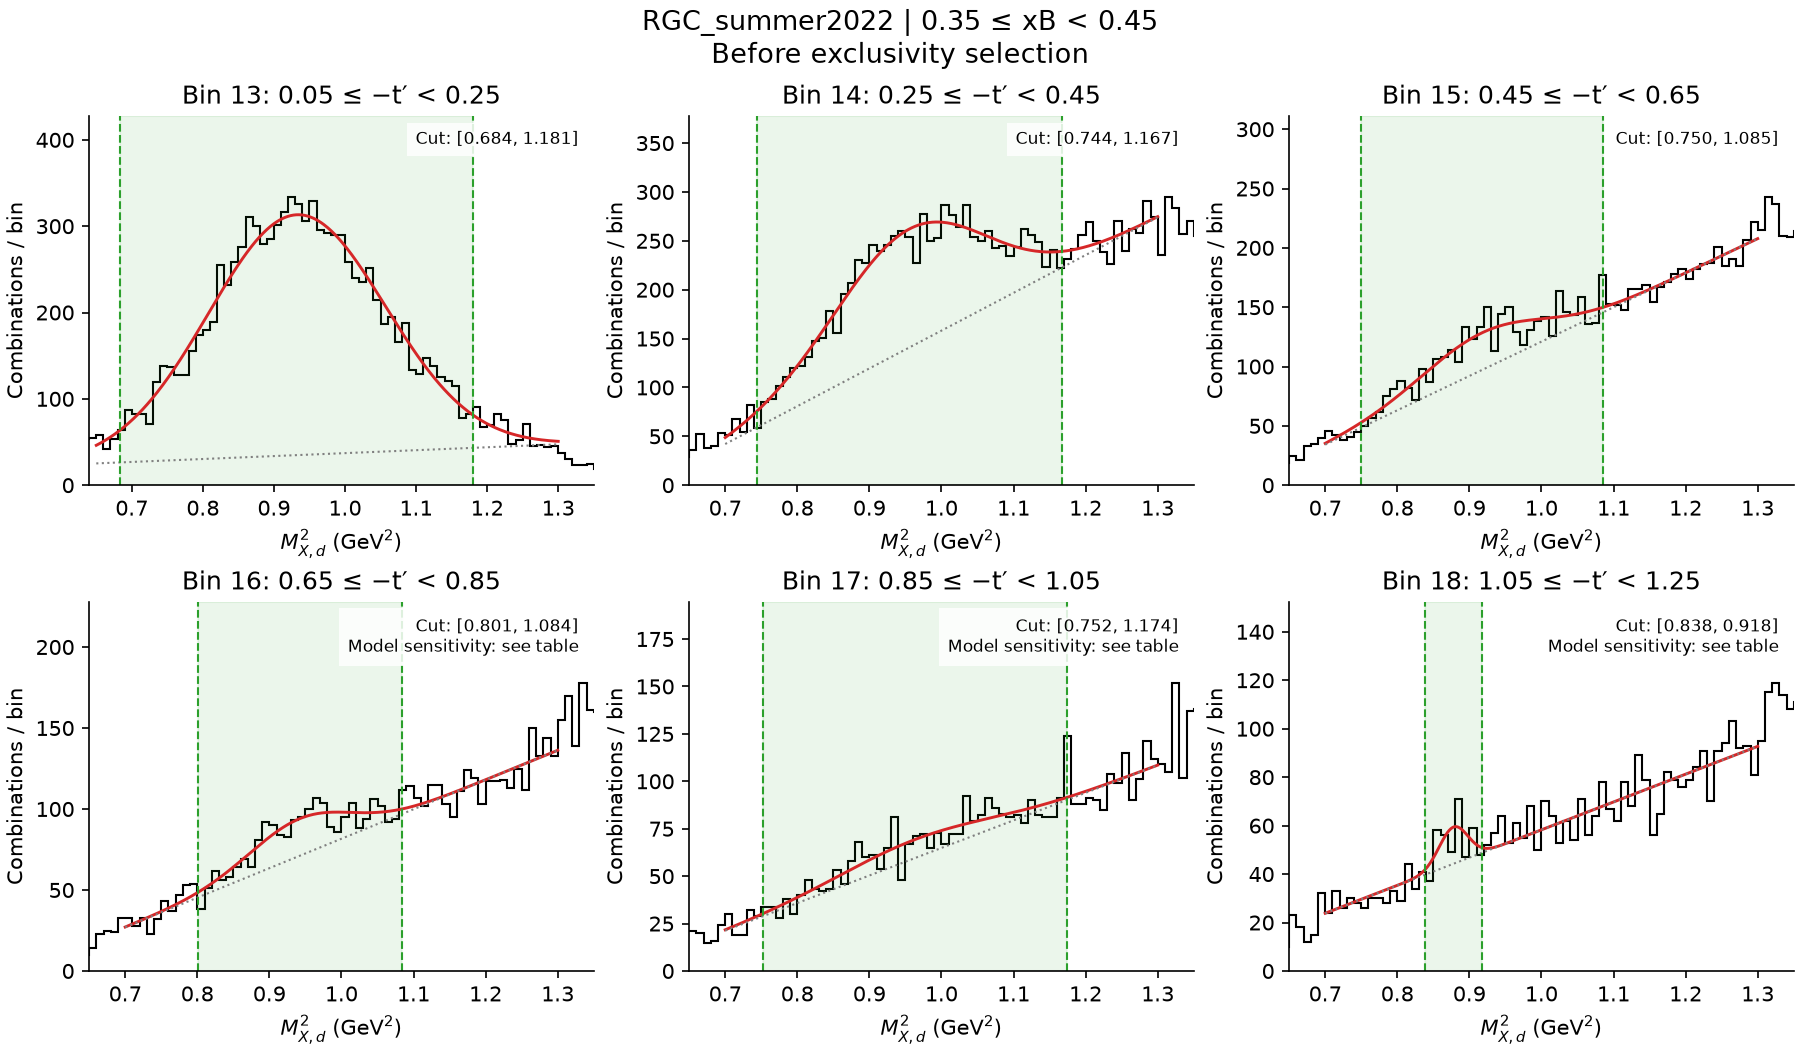
\includegraphics[width=\linewidth]{figures/channel_selection/exclusivity/rgc_su22_mass_xb3.png}
\caption{RGC\_summer2022: deuteron-reference missing-mass-squared fits in $x_B$ interval 3. The panels retain the six fine selection bins.}\label{fig:new_excl_rgc_su22_mass3}
\end{figure}
\clearpage
\begin{figure}[p]\centering
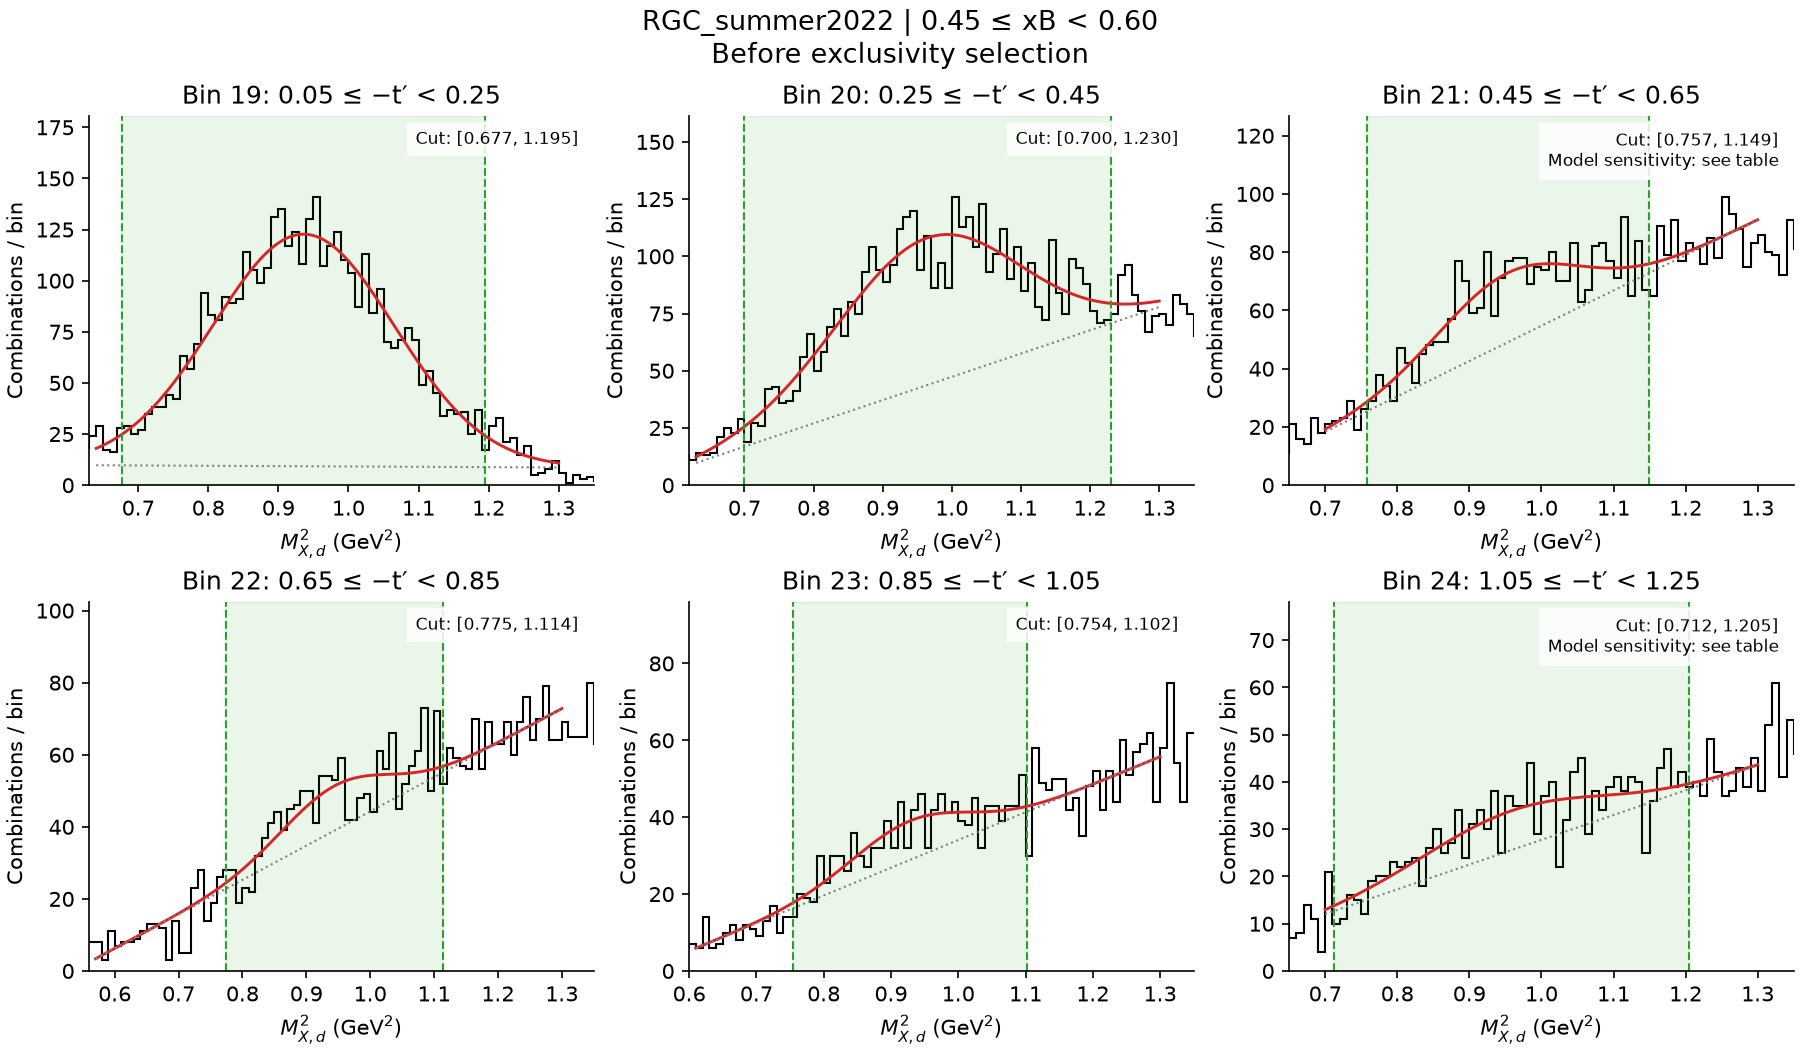
\includegraphics[width=\linewidth]{figures/channel_selection/exclusivity/rgc_su22_mass_xb4.png}
\caption{RGC\_summer2022: deuteron-reference missing-mass-squared fits in $x_B$ interval 4. The panels retain the six fine selection bins.}\label{fig:new_excl_rgc_su22_mass4}
\end{figure}
\clearpage
\begin{figure}[p]\centering
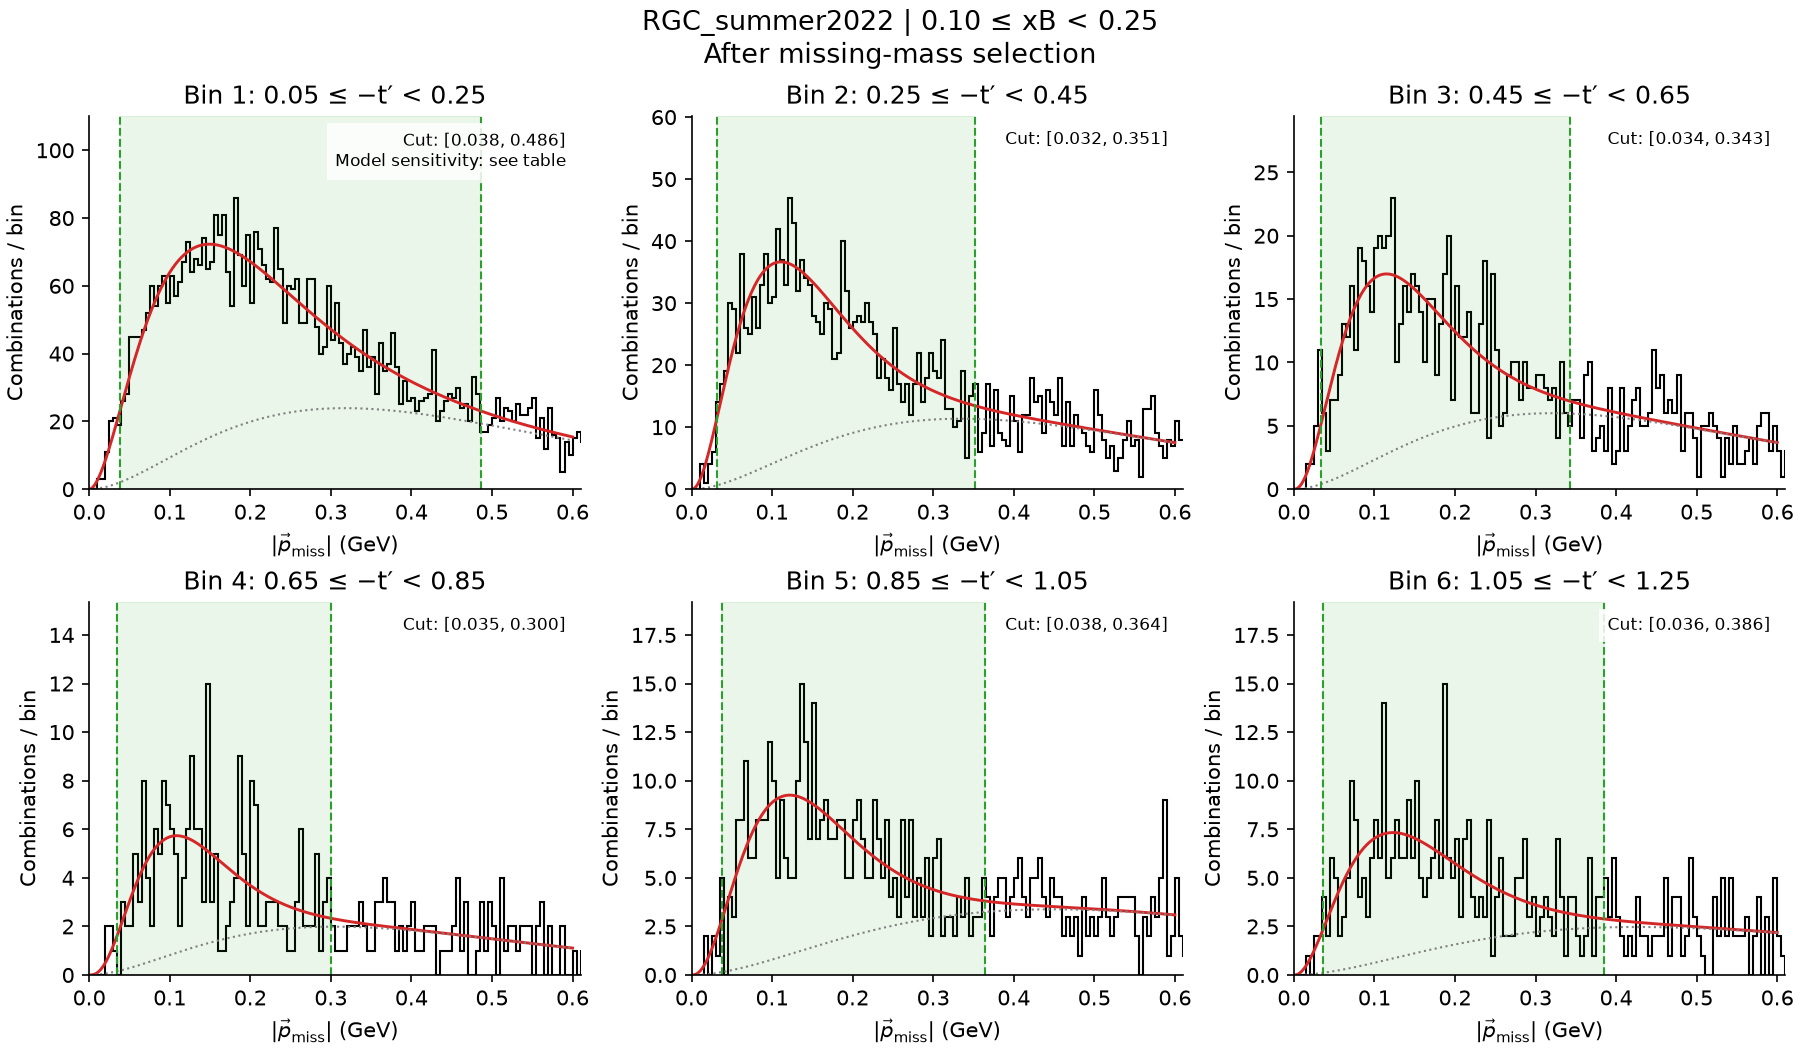
\includegraphics[width=\linewidth]{figures/channel_selection/exclusivity/rgc_su22_momentum_xb1.png}
\caption{RGC\_summer2022: missing-momentum fits after the mass cut in $x_B$ interval 1. The panels retain the six fine selection bins.}\label{fig:new_excl_rgc_su22_momentum1}
\end{figure}
\clearpage
\begin{figure}[p]\centering
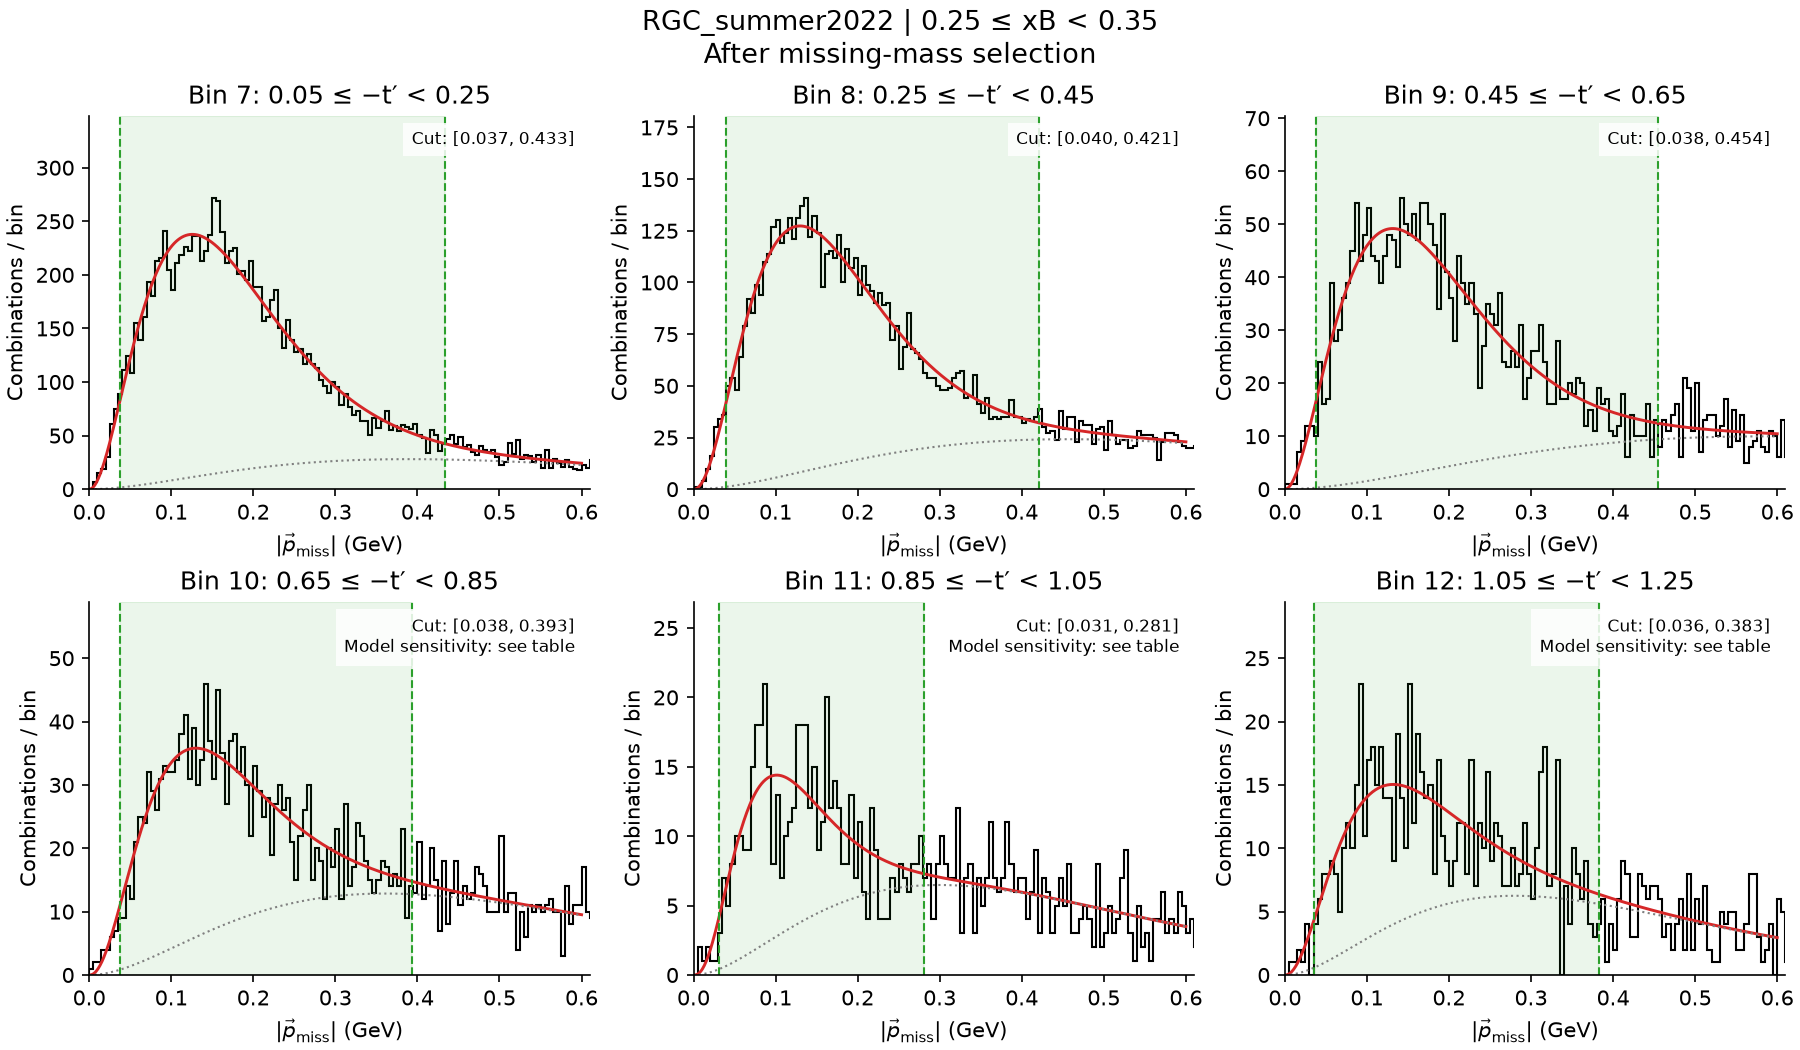
\includegraphics[width=\linewidth]{figures/channel_selection/exclusivity/rgc_su22_momentum_xb2.png}
\caption{RGC\_summer2022: missing-momentum fits after the mass cut in $x_B$ interval 2. The panels retain the six fine selection bins.}\label{fig:new_excl_rgc_su22_momentum2}
\end{figure}
\clearpage
\begin{figure}[p]\centering
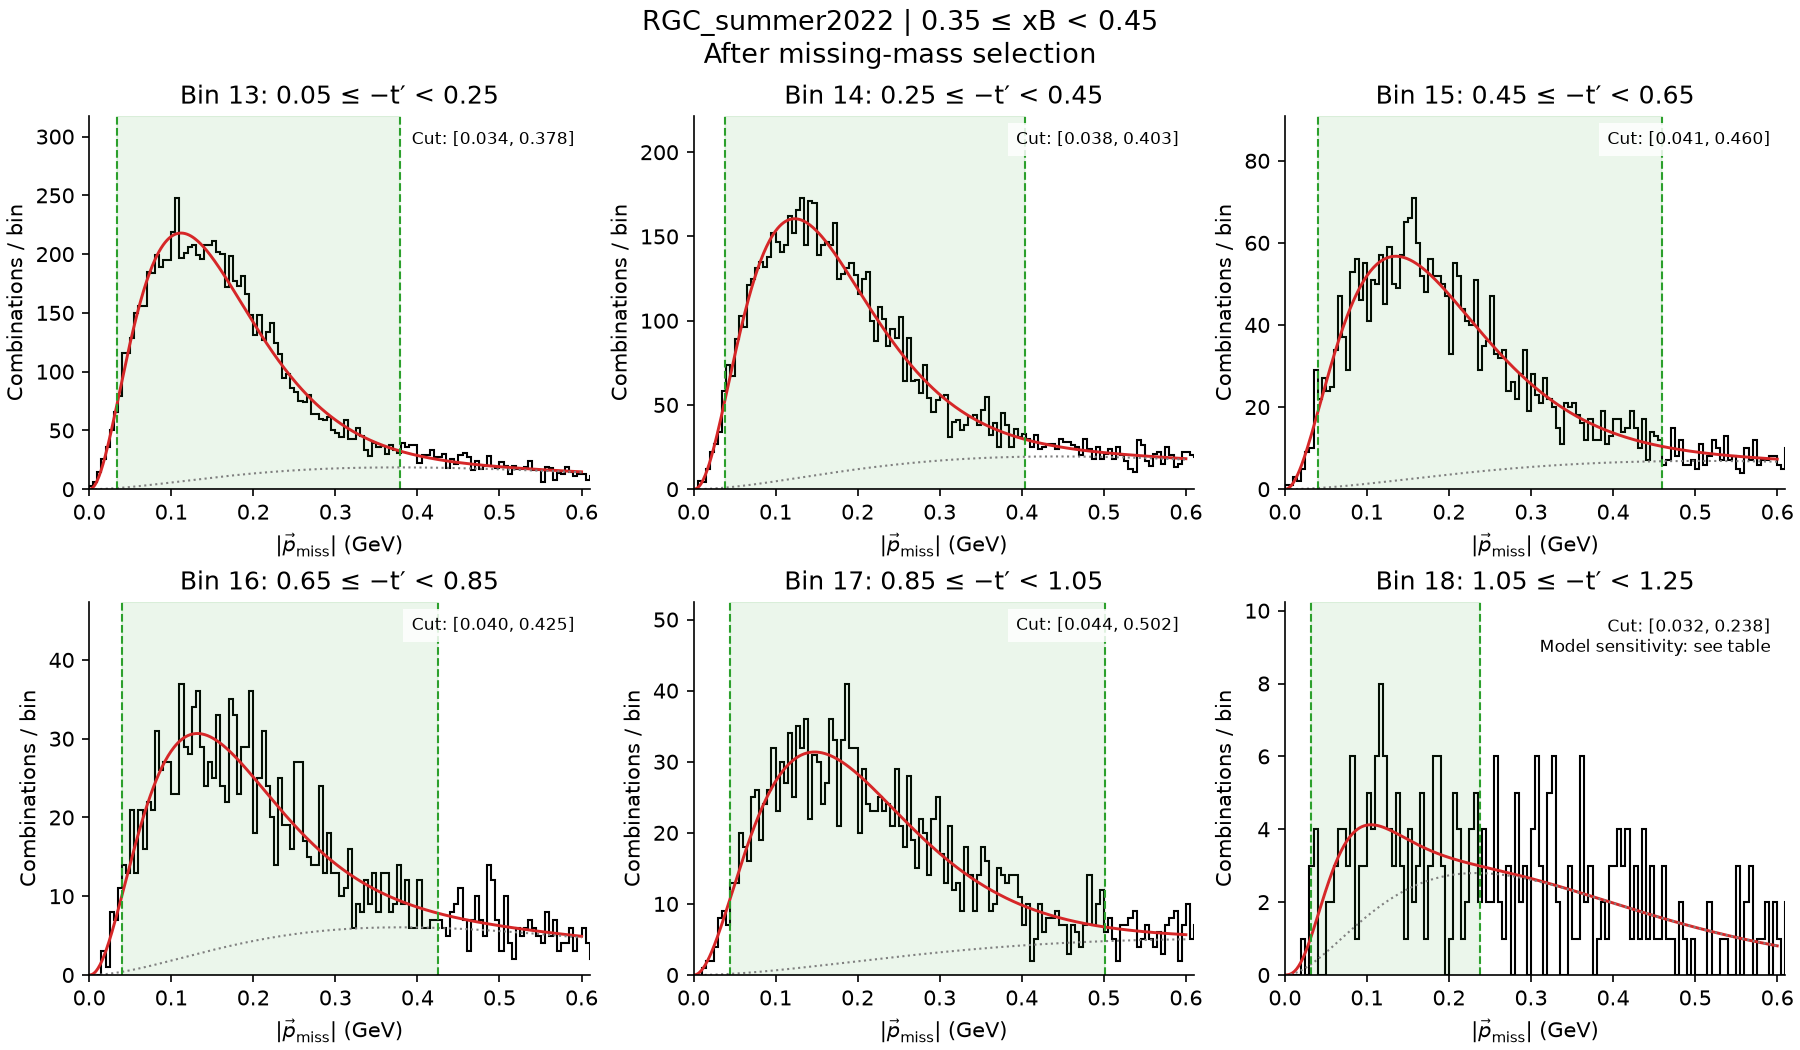
\includegraphics[width=\linewidth]{figures/channel_selection/exclusivity/rgc_su22_momentum_xb3.png}
\caption{RGC\_summer2022: missing-momentum fits after the mass cut in $x_B$ interval 3. The panels retain the six fine selection bins.}\label{fig:new_excl_rgc_su22_momentum3}
\end{figure}
\clearpage
\begin{figure}[p]\centering
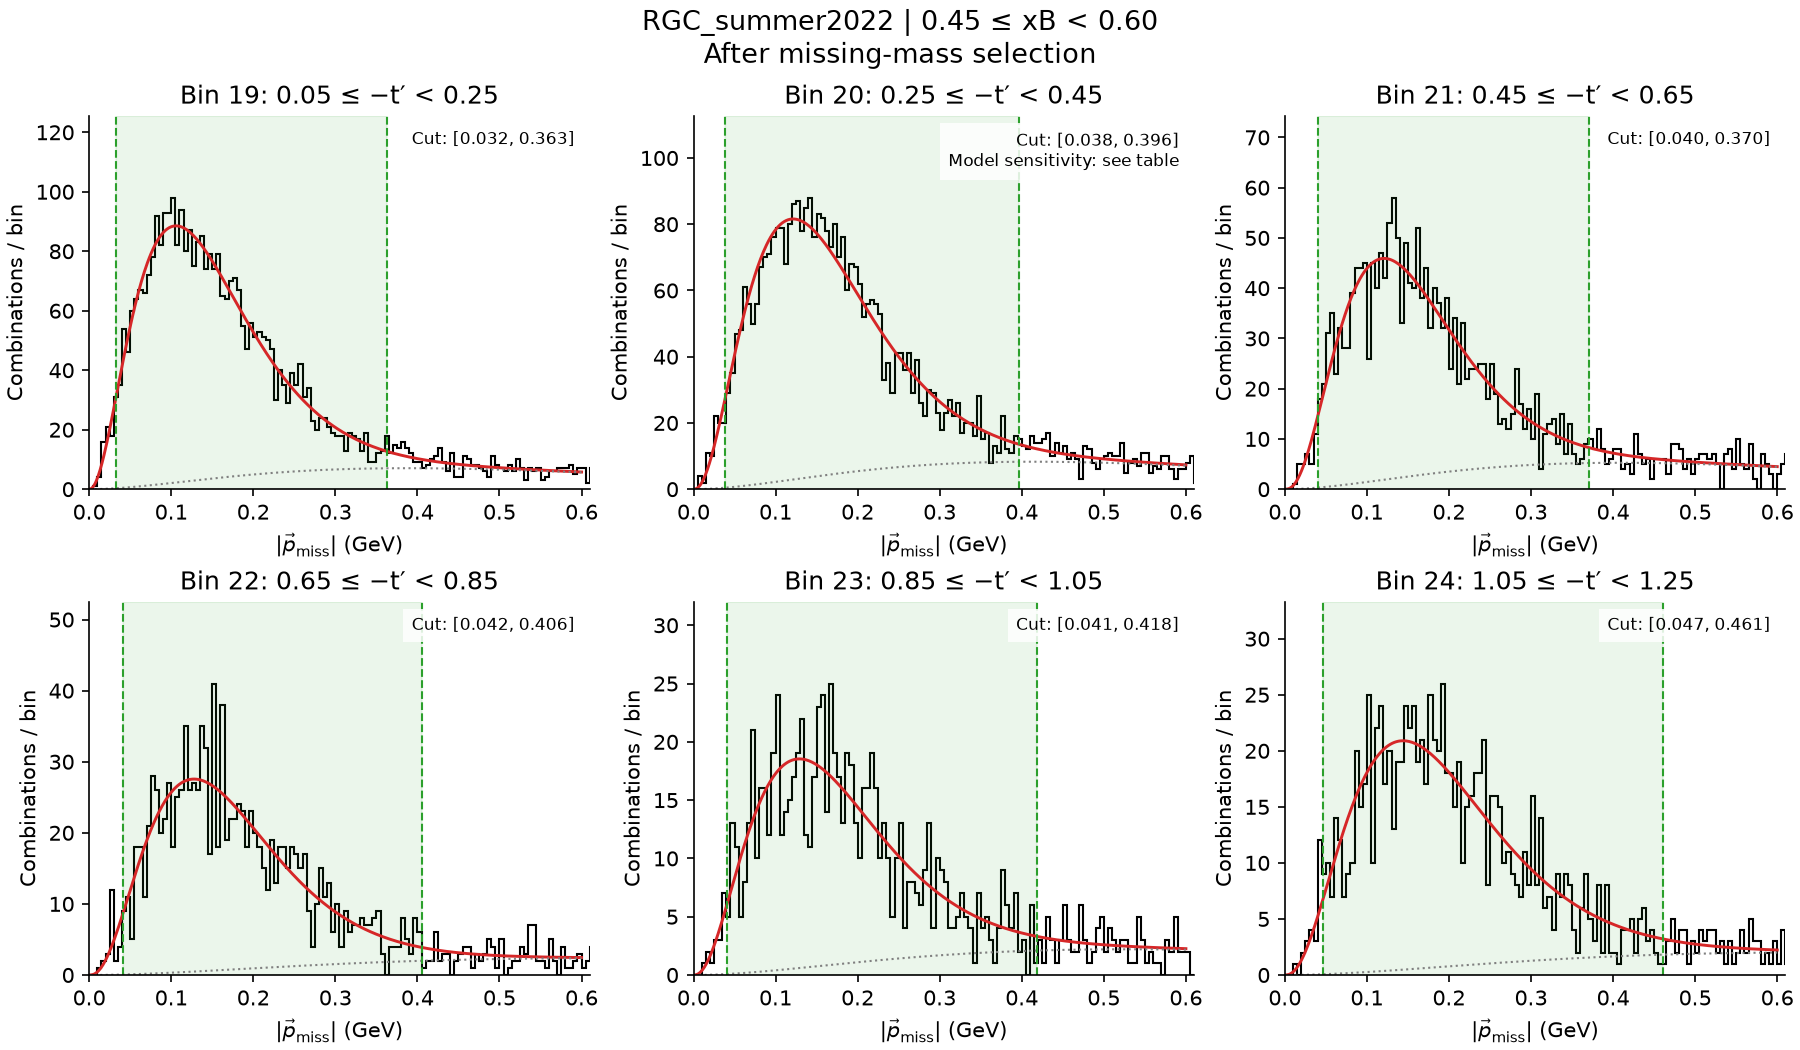
\includegraphics[width=\linewidth]{figures/channel_selection/exclusivity/rgc_su22_momentum_xb4.png}
\caption{RGC\_summer2022: missing-momentum fits after the mass cut in $x_B$ interval 4. The panels retain the six fine selection bins.}\label{fig:new_excl_rgc_su22_momentum4}
\end{figure}
\clearpage
\begin{figure}[p]\centering
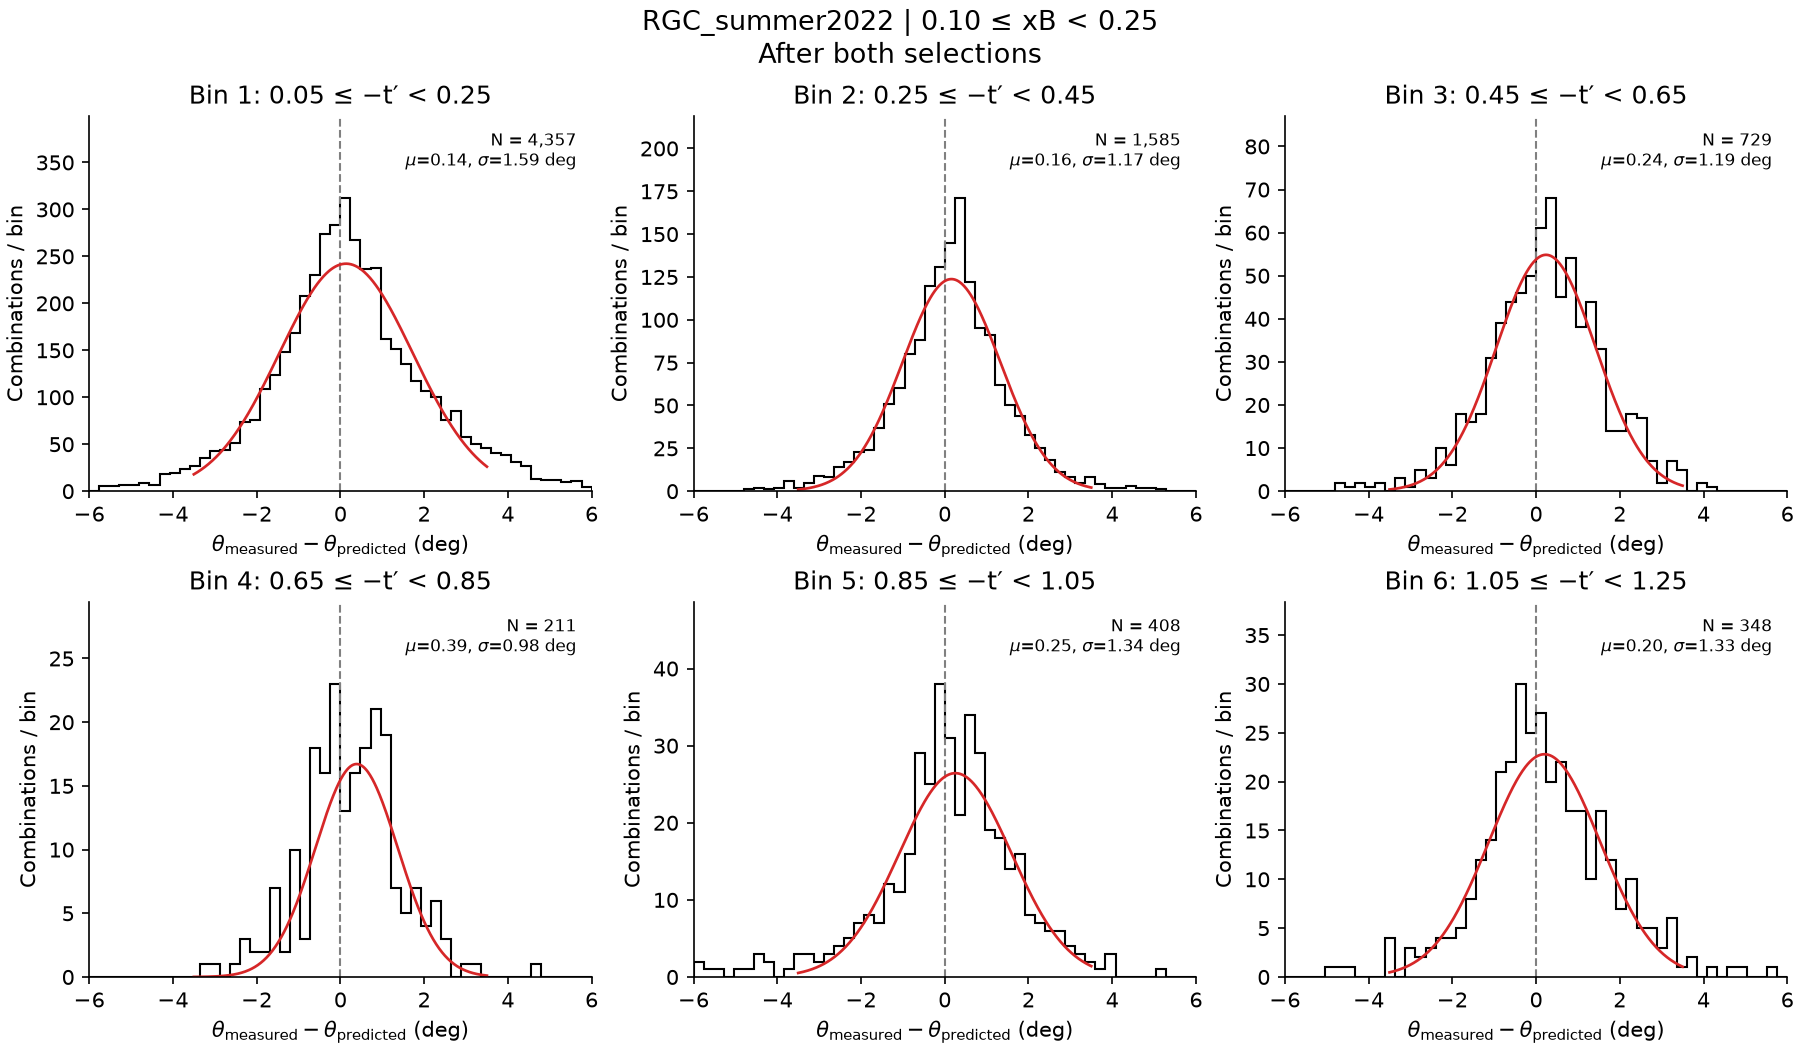
\includegraphics[width=\linewidth]{figures/channel_selection/exclusivity/rgc_su22_angle_xb1.png}
\caption{RGC\_summer2022: pion polar-angle closure after both cuts in $x_B$ interval 1. The panels retain the six fine selection bins.}\label{fig:new_excl_rgc_su22_angle1}
\end{figure}
\clearpage
\begin{figure}[p]\centering
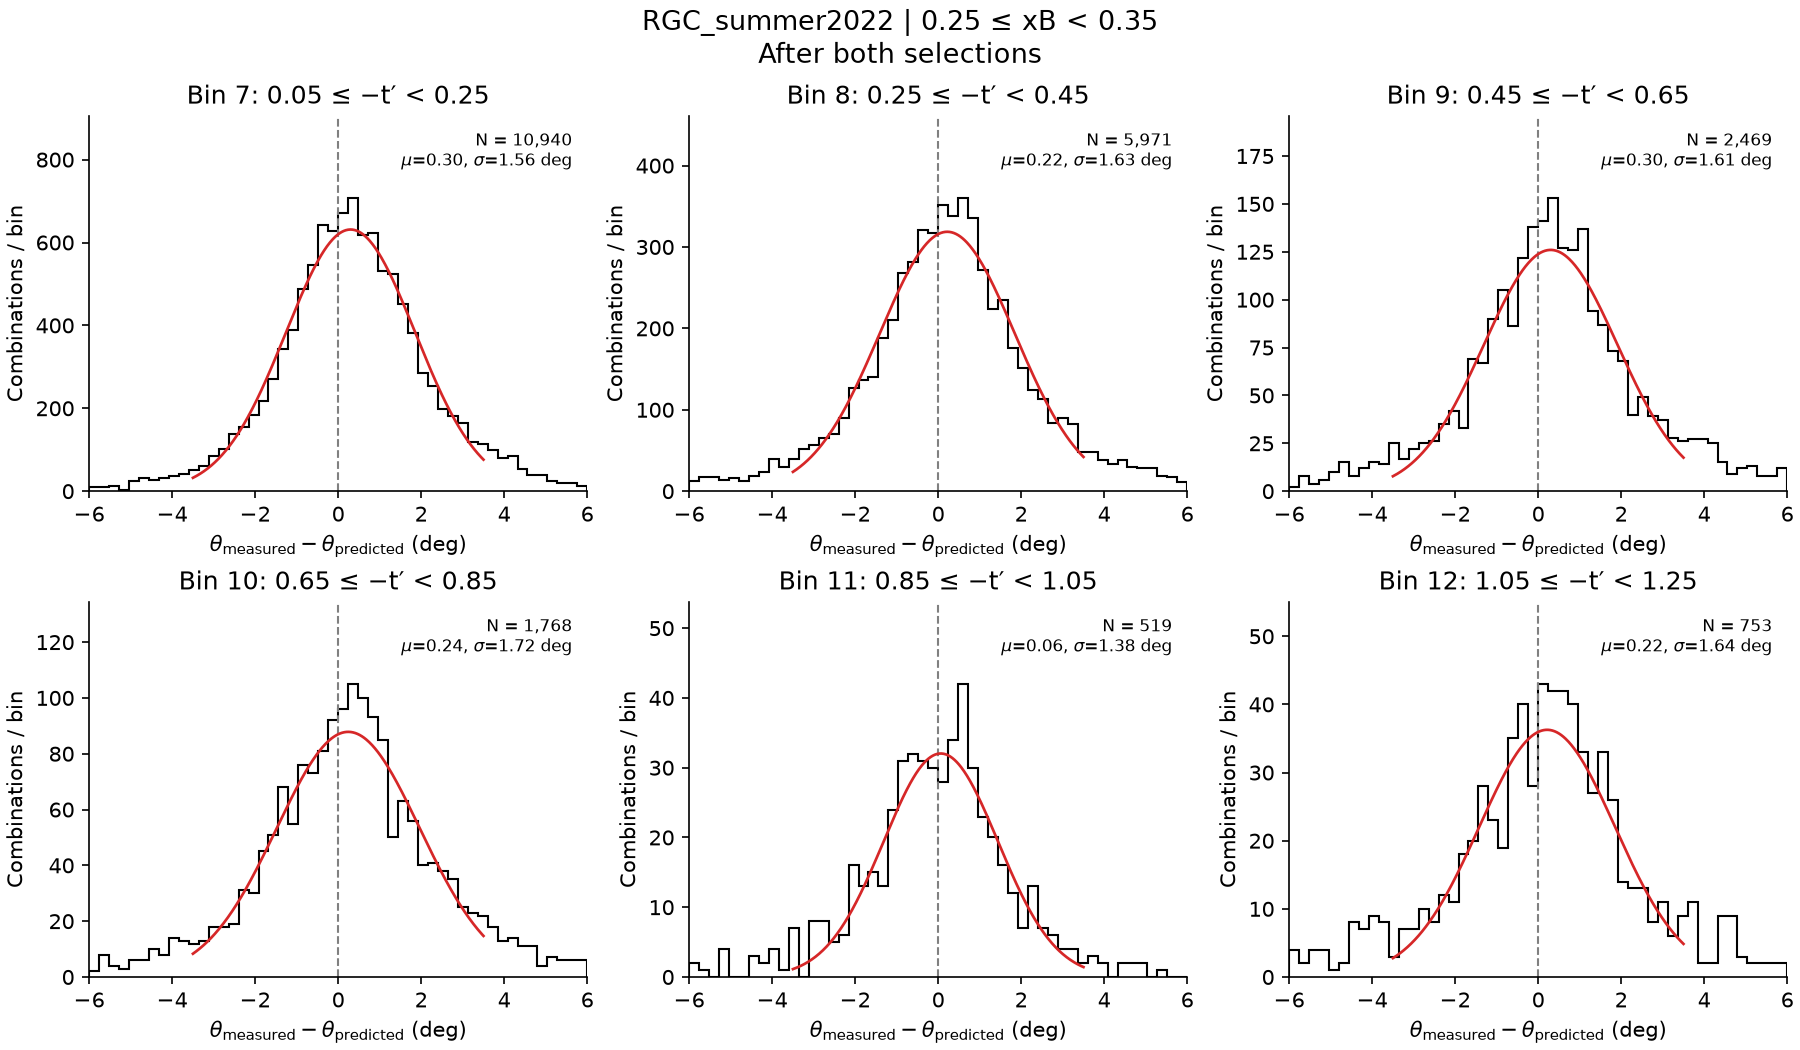
\includegraphics[width=\linewidth]{figures/channel_selection/exclusivity/rgc_su22_angle_xb2.png}
\caption{RGC\_summer2022: pion polar-angle closure after both cuts in $x_B$ interval 2. The panels retain the six fine selection bins.}\label{fig:new_excl_rgc_su22_angle2}
\end{figure}
\clearpage
\begin{figure}[p]\centering
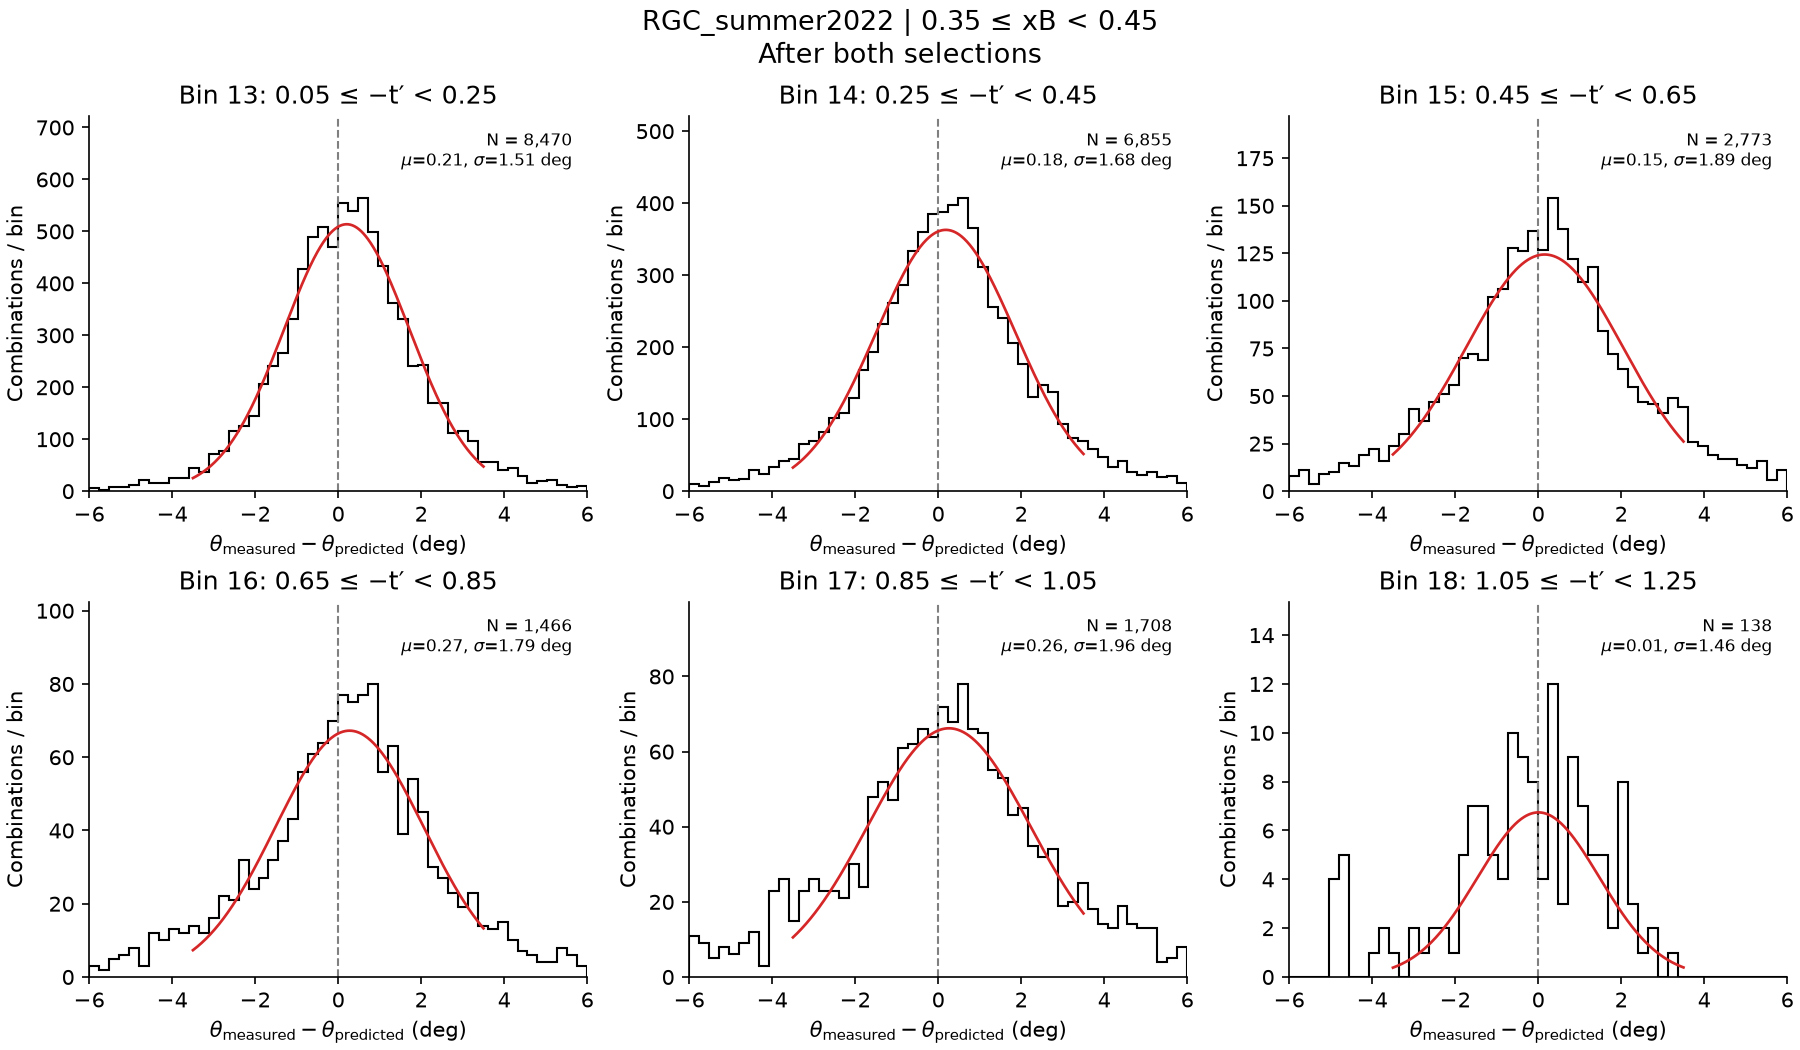
\includegraphics[width=\linewidth]{figures/channel_selection/exclusivity/rgc_su22_angle_xb3.png}
\caption{RGC\_summer2022: pion polar-angle closure after both cuts in $x_B$ interval 3. The panels retain the six fine selection bins.}\label{fig:new_excl_rgc_su22_angle3}
\end{figure}
\clearpage
\begin{figure}[p]\centering
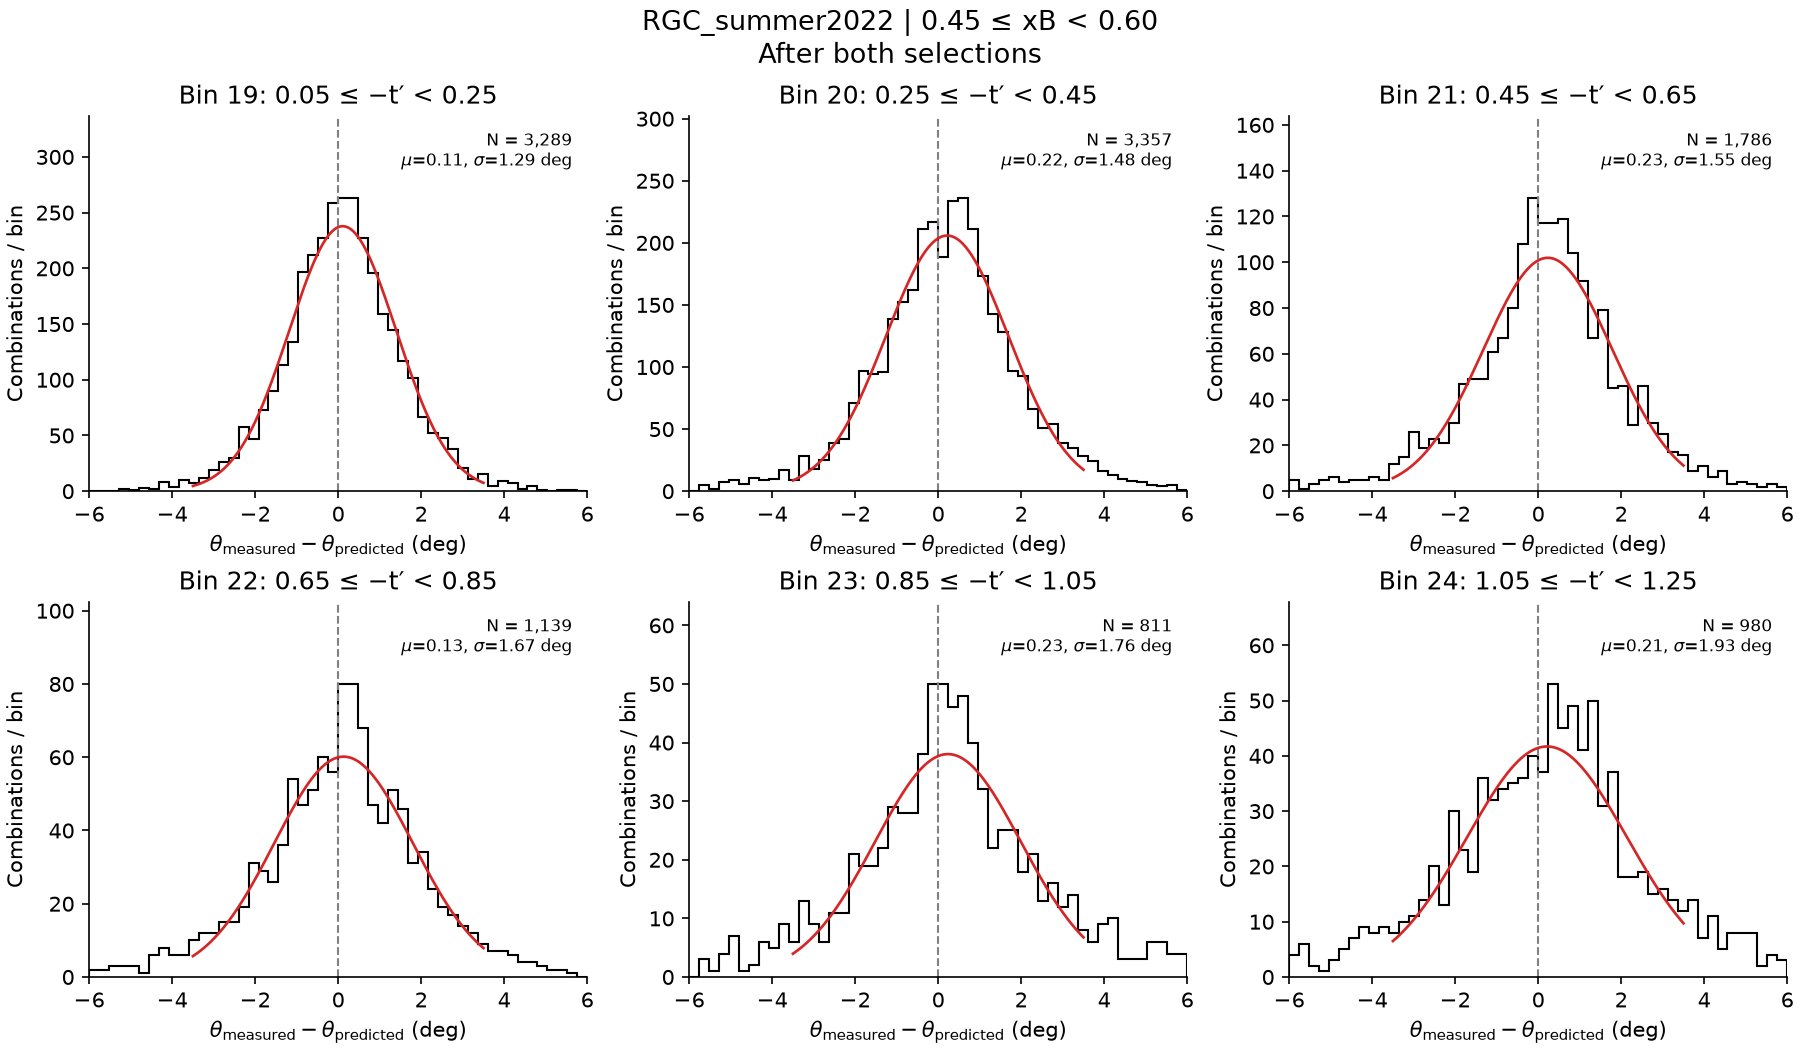
\includegraphics[width=\linewidth]{figures/channel_selection/exclusivity/rgc_su22_angle_xb4.png}
\caption{RGC\_summer2022: pion polar-angle closure after both cuts in $x_B$ interval 4. The panels retain the six fine selection bins.}\label{fig:new_excl_rgc_su22_angle4}
\end{figure}
\clearpage
\begin{figure}[p]\centering
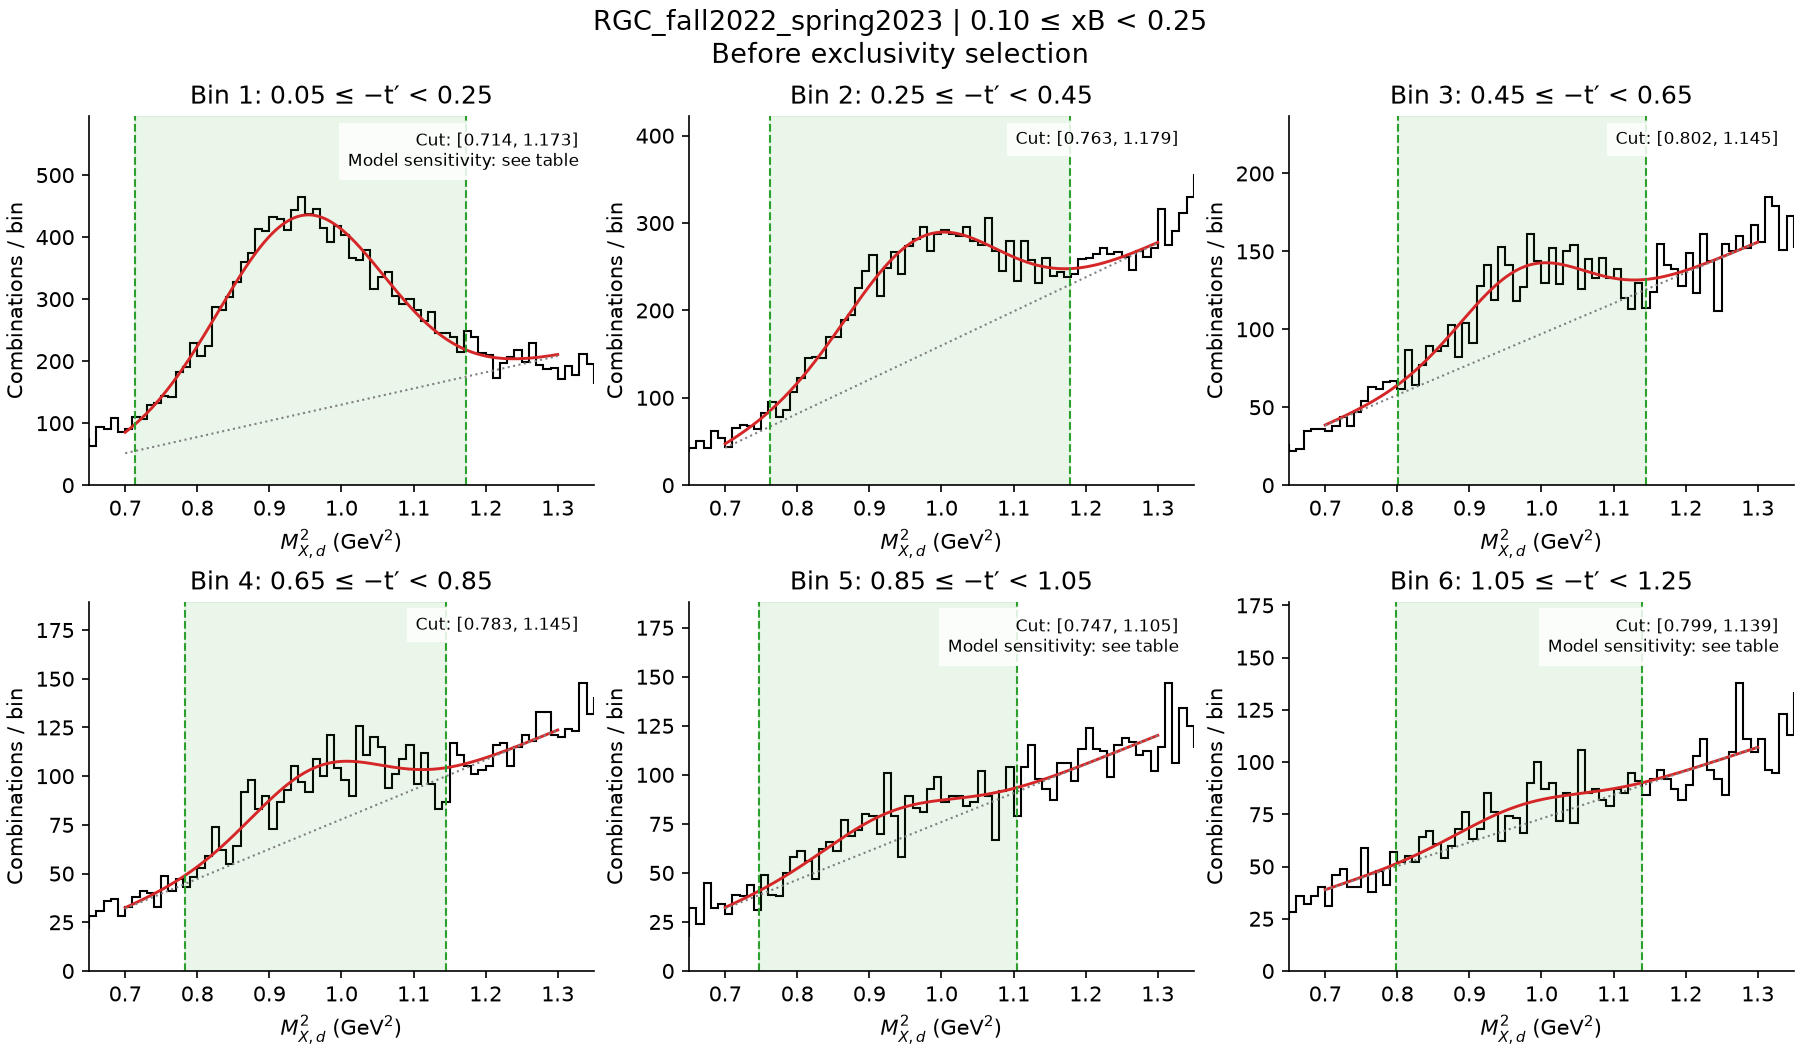
\includegraphics[width=\linewidth]{figures/channel_selection/exclusivity/rgc_fa22_sp23_mass_xb1.png}
\caption{RGC\_fall2022\_spring2023: deuteron-reference missing-mass-squared fits in $x_B$ interval 1. The panels retain the six fine selection bins.}\label{fig:new_excl_rgc_fa22_sp23_mass1}
\end{figure}
\clearpage
\begin{figure}[p]\centering
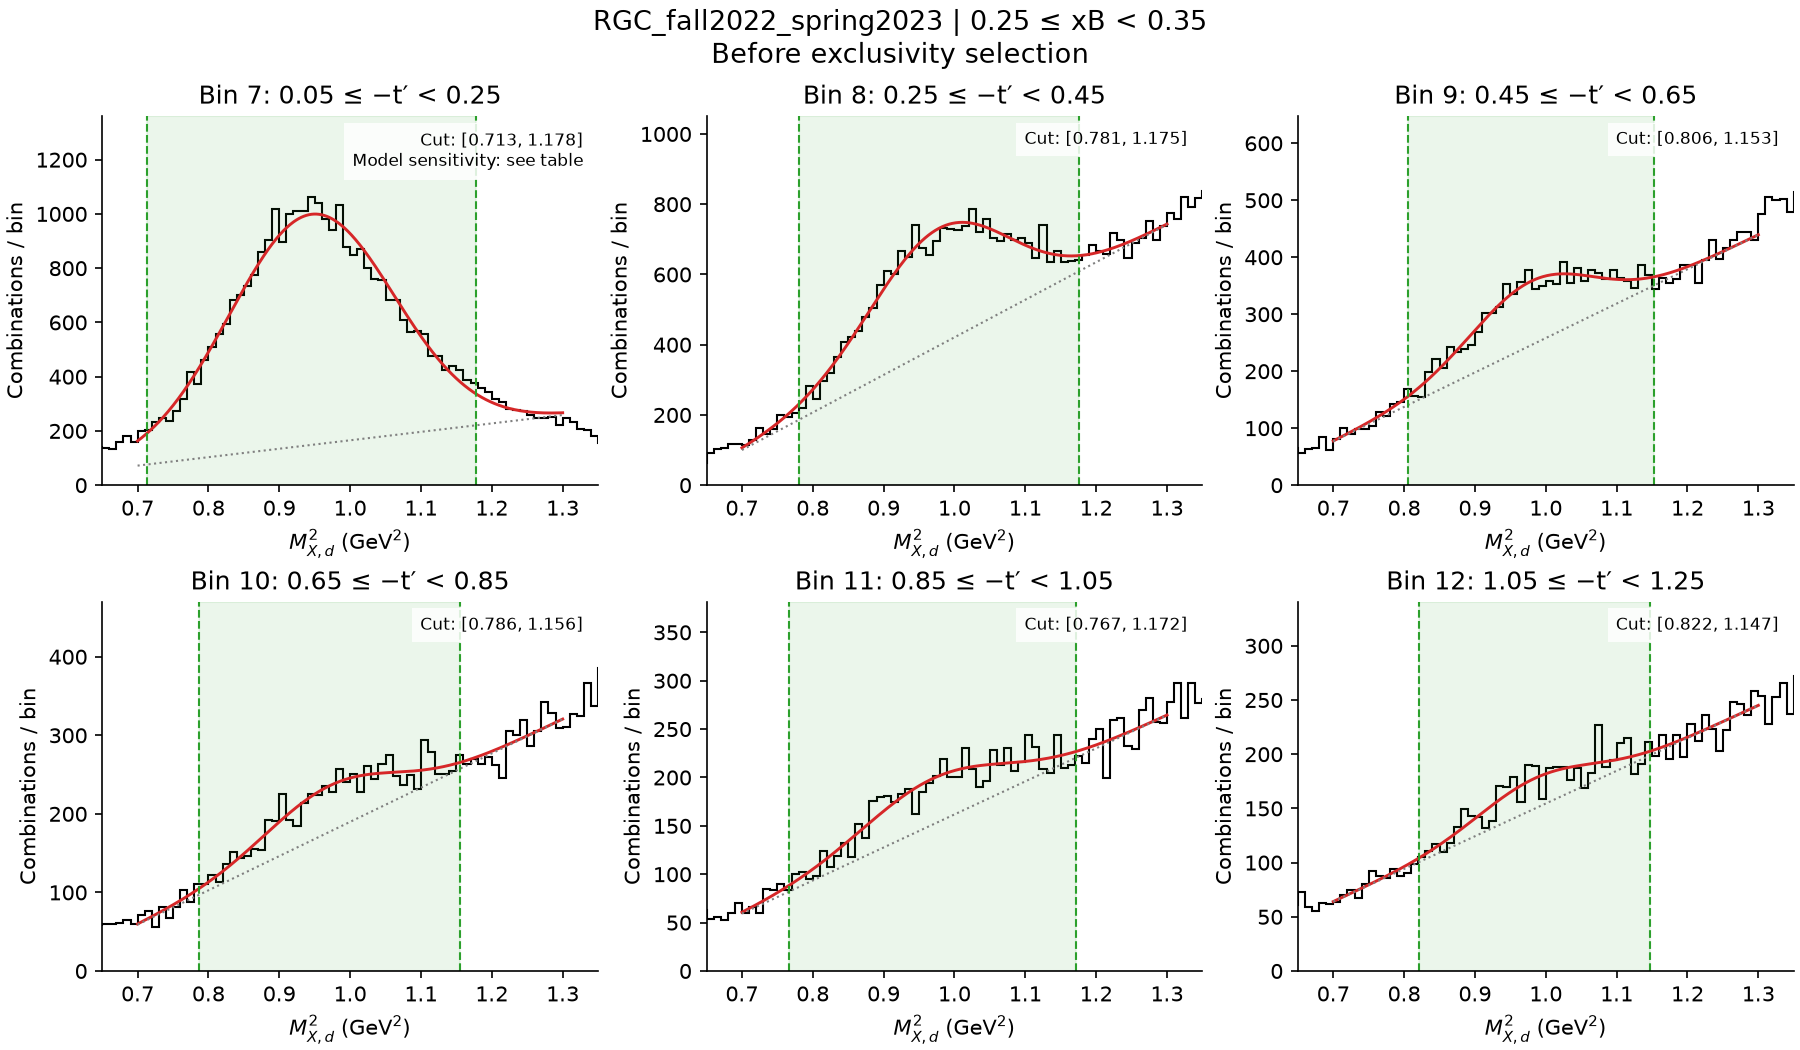
\includegraphics[width=\linewidth]{figures/channel_selection/exclusivity/rgc_fa22_sp23_mass_xb2.png}
\caption{RGC\_fall2022\_spring2023: deuteron-reference missing-mass-squared fits in $x_B$ interval 2. The panels retain the six fine selection bins.}\label{fig:new_excl_rgc_fa22_sp23_mass2}
\end{figure}
\clearpage
\begin{figure}[p]\centering
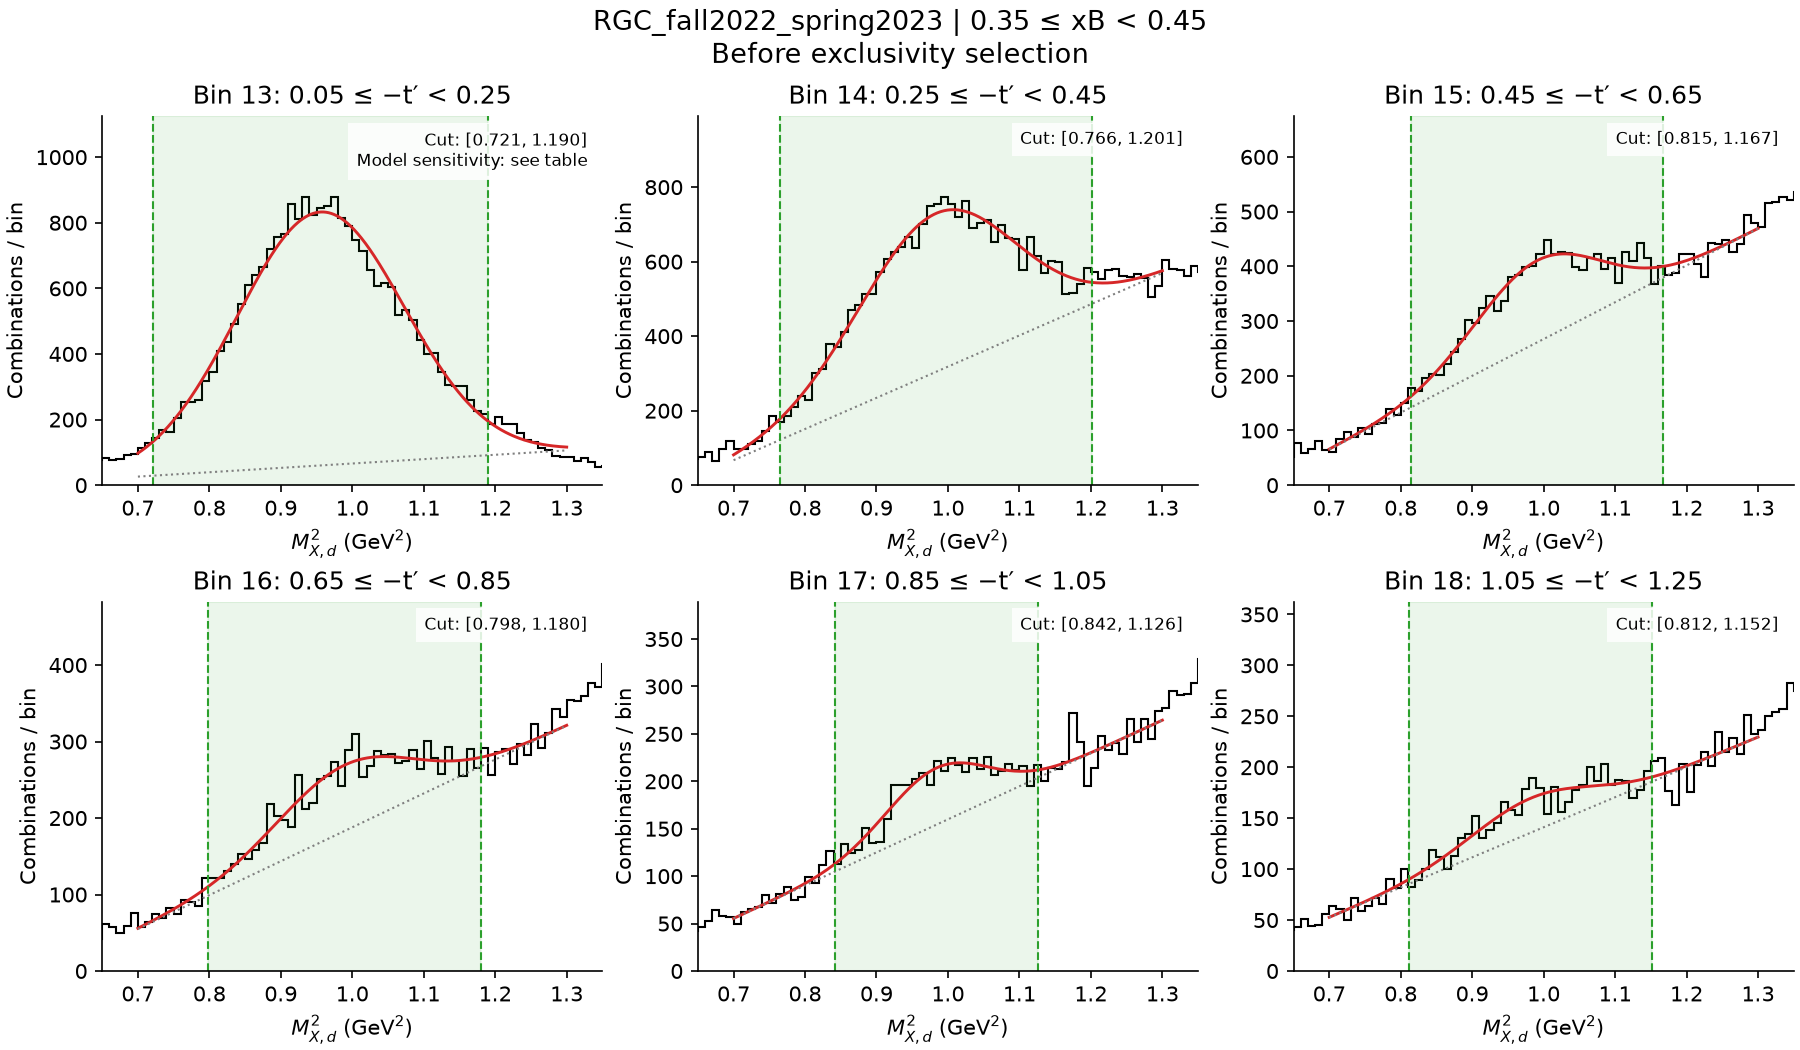
\includegraphics[width=\linewidth]{figures/channel_selection/exclusivity/rgc_fa22_sp23_mass_xb3.png}
\caption{RGC\_fall2022\_spring2023: deuteron-reference missing-mass-squared fits in $x_B$ interval 3. The panels retain the six fine selection bins.}\label{fig:new_excl_rgc_fa22_sp23_mass3}
\end{figure}
\clearpage
\begin{figure}[p]\centering
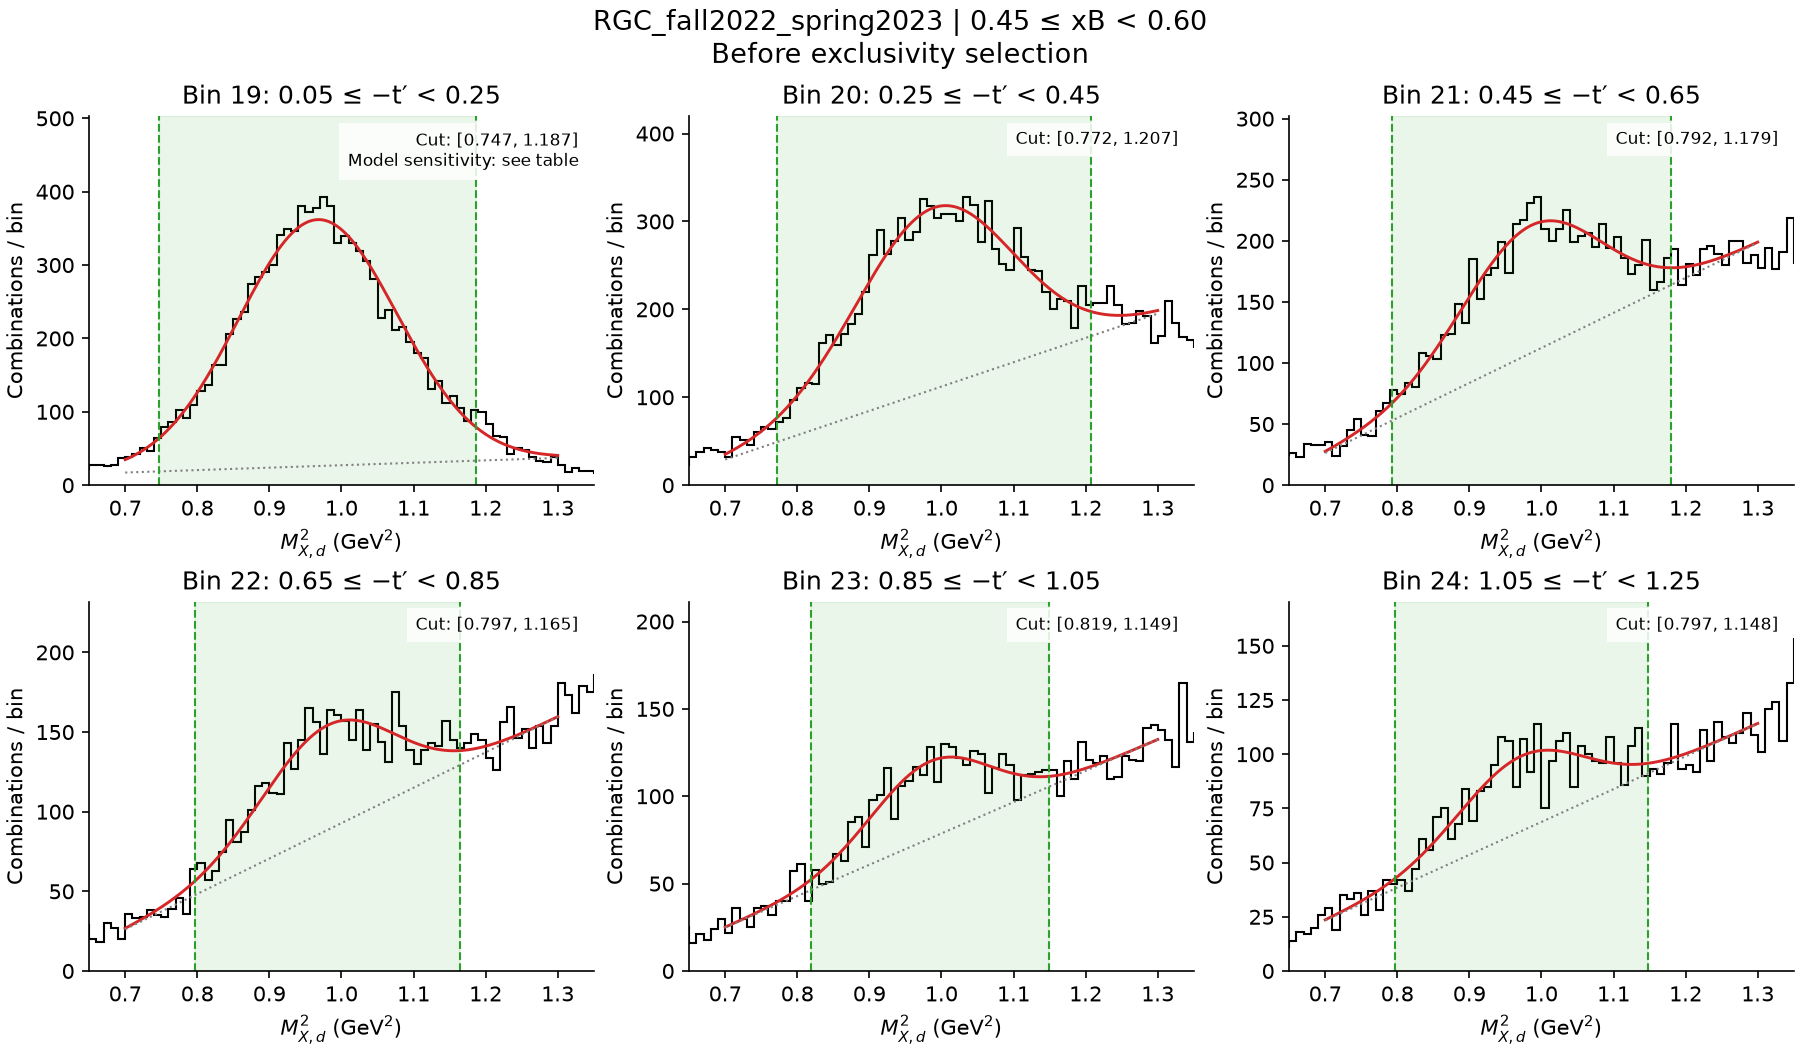
\includegraphics[width=\linewidth]{figures/channel_selection/exclusivity/rgc_fa22_sp23_mass_xb4.png}
\caption{RGC\_fall2022\_spring2023: deuteron-reference missing-mass-squared fits in $x_B$ interval 4. The panels retain the six fine selection bins.}\label{fig:new_excl_rgc_fa22_sp23_mass4}
\end{figure}
\clearpage
\begin{figure}[p]\centering
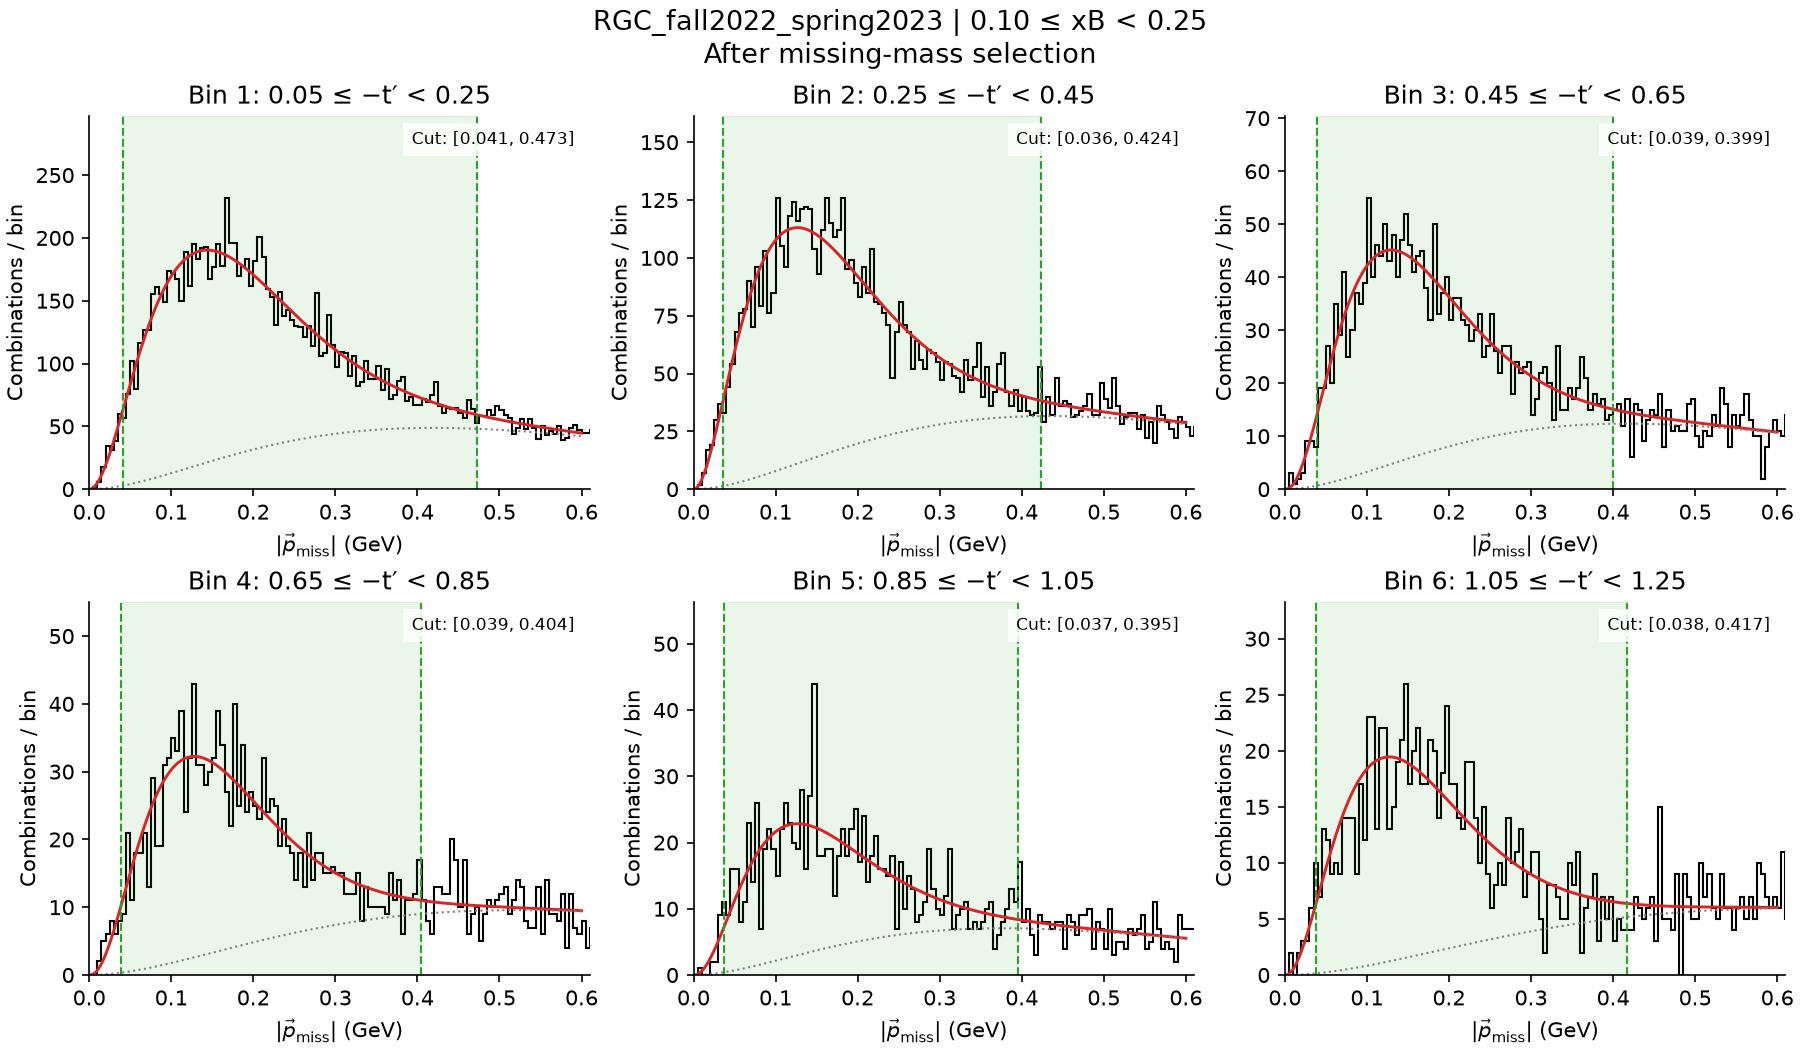
\includegraphics[width=\linewidth]{figures/channel_selection/exclusivity/rgc_fa22_sp23_momentum_xb1.png}
\caption{RGC\_fall2022\_spring2023: missing-momentum fits after the mass cut in $x_B$ interval 1. The panels retain the six fine selection bins.}\label{fig:new_excl_rgc_fa22_sp23_momentum1}
\end{figure}
\clearpage
\begin{figure}[p]\centering
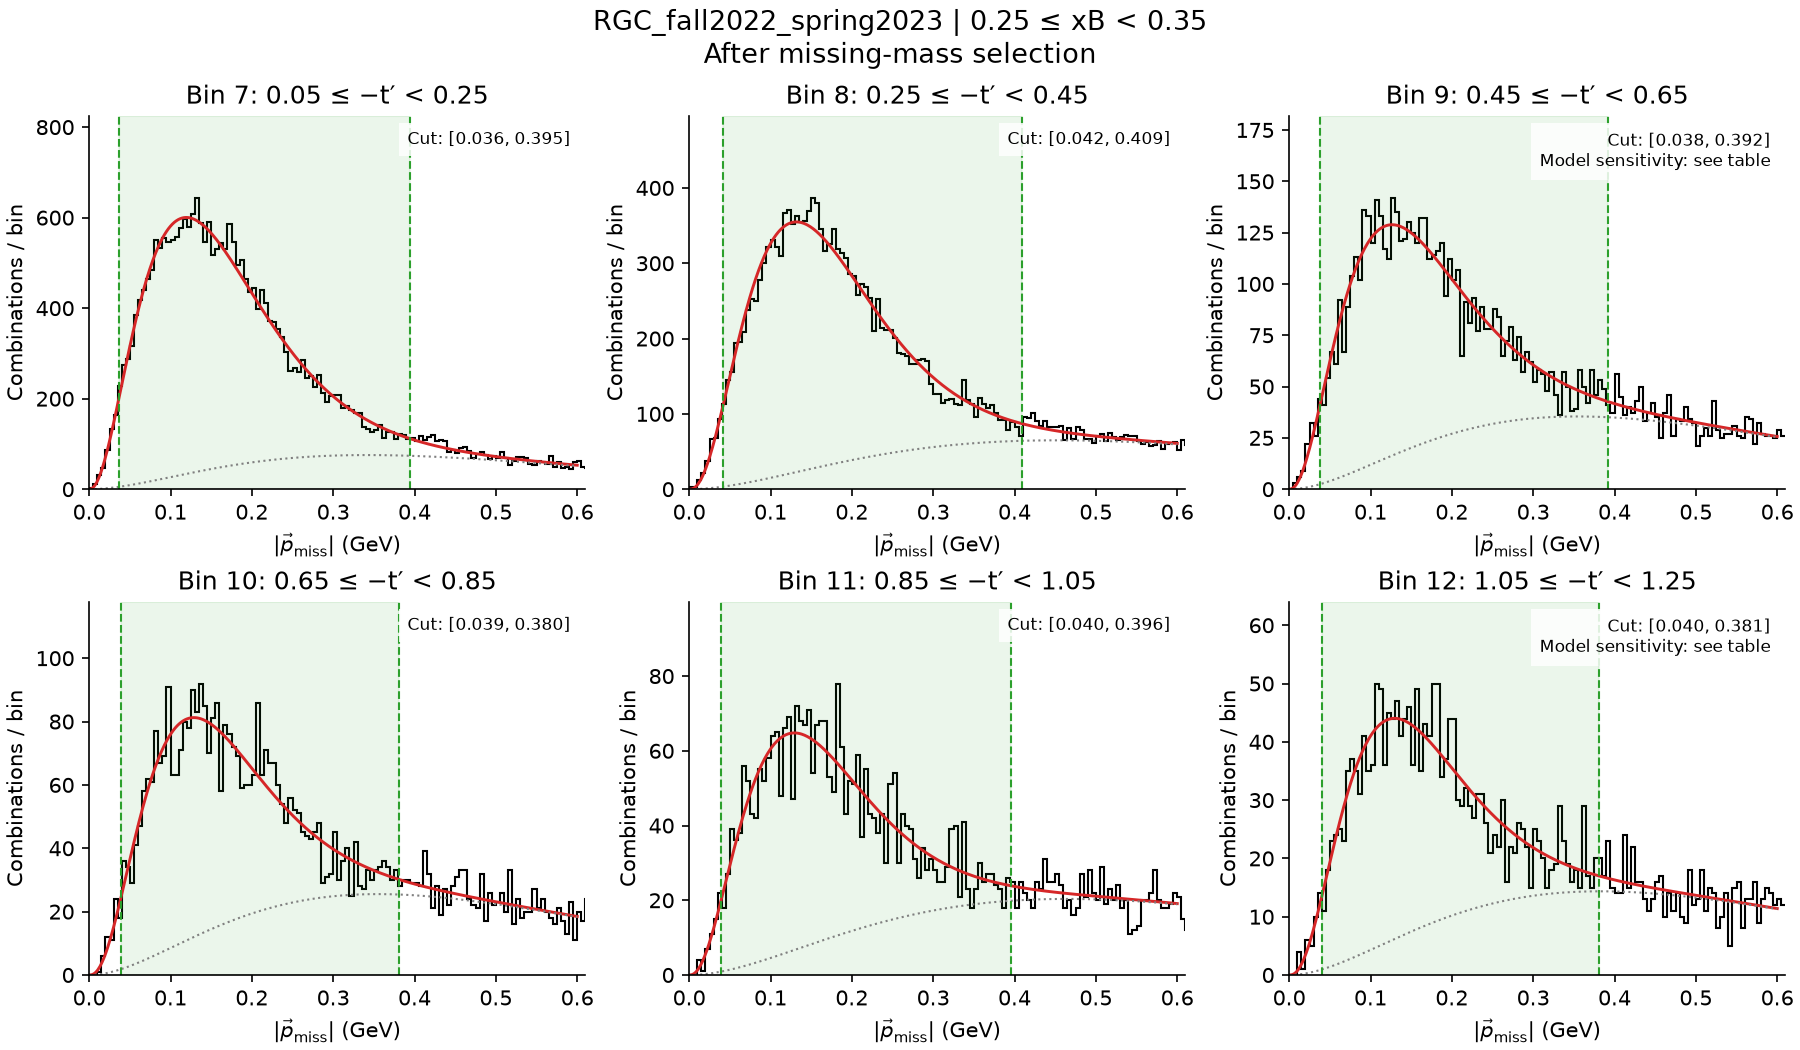
\includegraphics[width=\linewidth]{figures/channel_selection/exclusivity/rgc_fa22_sp23_momentum_xb2.png}
\caption{RGC\_fall2022\_spring2023: missing-momentum fits after the mass cut in $x_B$ interval 2. The panels retain the six fine selection bins.}\label{fig:new_excl_rgc_fa22_sp23_momentum2}
\end{figure}
\clearpage
\begin{figure}[p]\centering
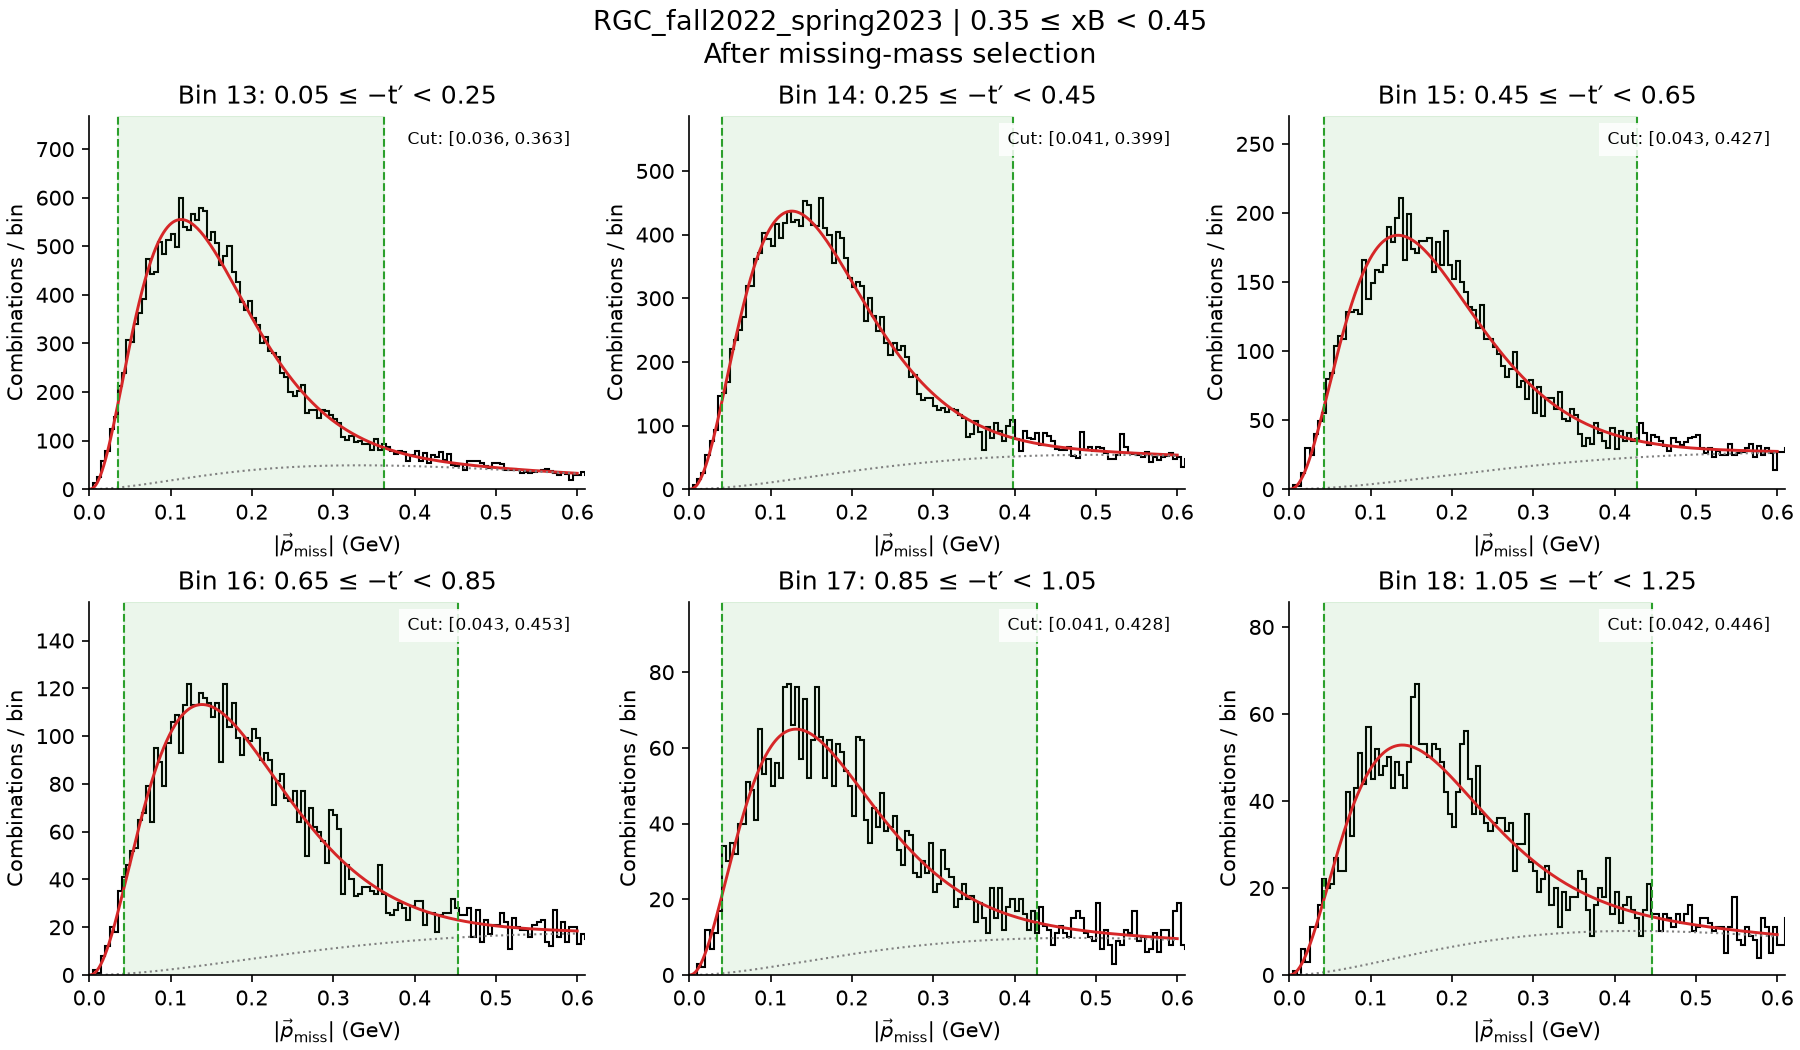
\includegraphics[width=\linewidth]{figures/channel_selection/exclusivity/rgc_fa22_sp23_momentum_xb3.png}
\caption{RGC\_fall2022\_spring2023: missing-momentum fits after the mass cut in $x_B$ interval 3. The panels retain the six fine selection bins.}\label{fig:new_excl_rgc_fa22_sp23_momentum3}
\end{figure}
\clearpage
\begin{figure}[p]\centering
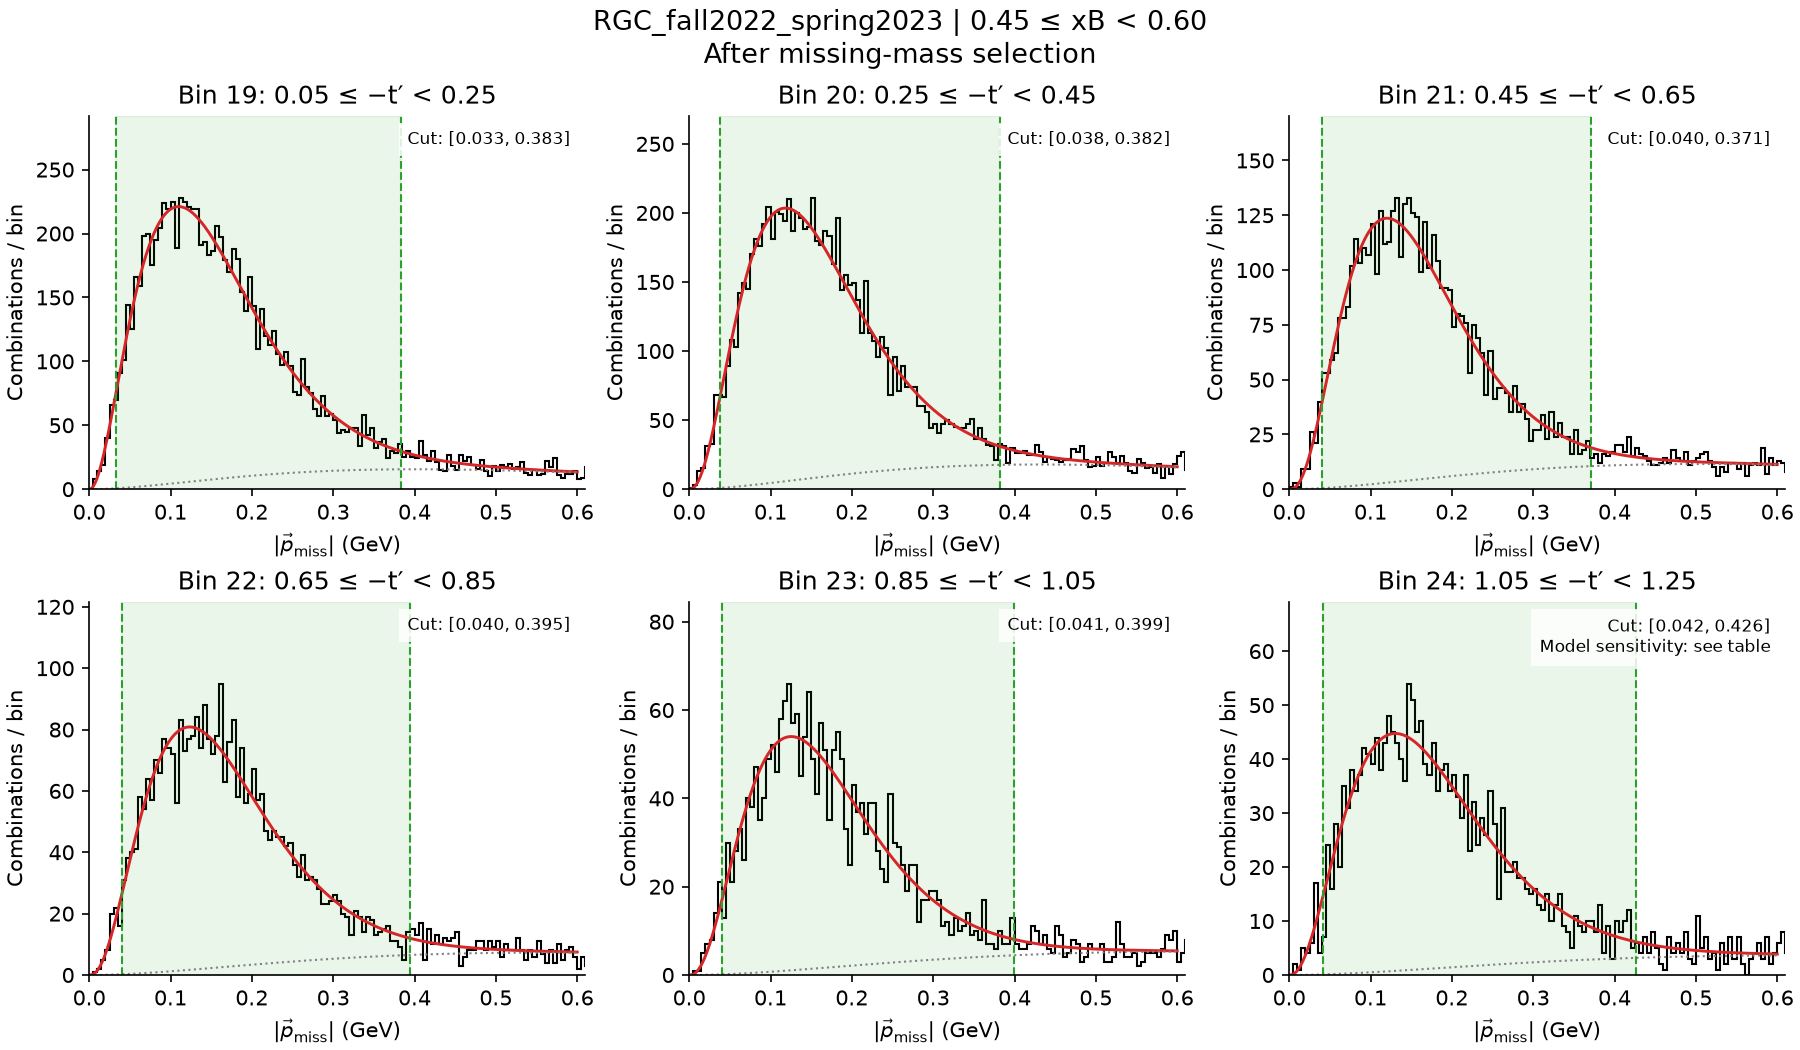
\includegraphics[width=\linewidth]{figures/channel_selection/exclusivity/rgc_fa22_sp23_momentum_xb4.png}
\caption{RGC\_fall2022\_spring2023: missing-momentum fits after the mass cut in $x_B$ interval 4. The panels retain the six fine selection bins.}\label{fig:new_excl_rgc_fa22_sp23_momentum4}
\end{figure}
\clearpage
\begin{figure}[p]\centering
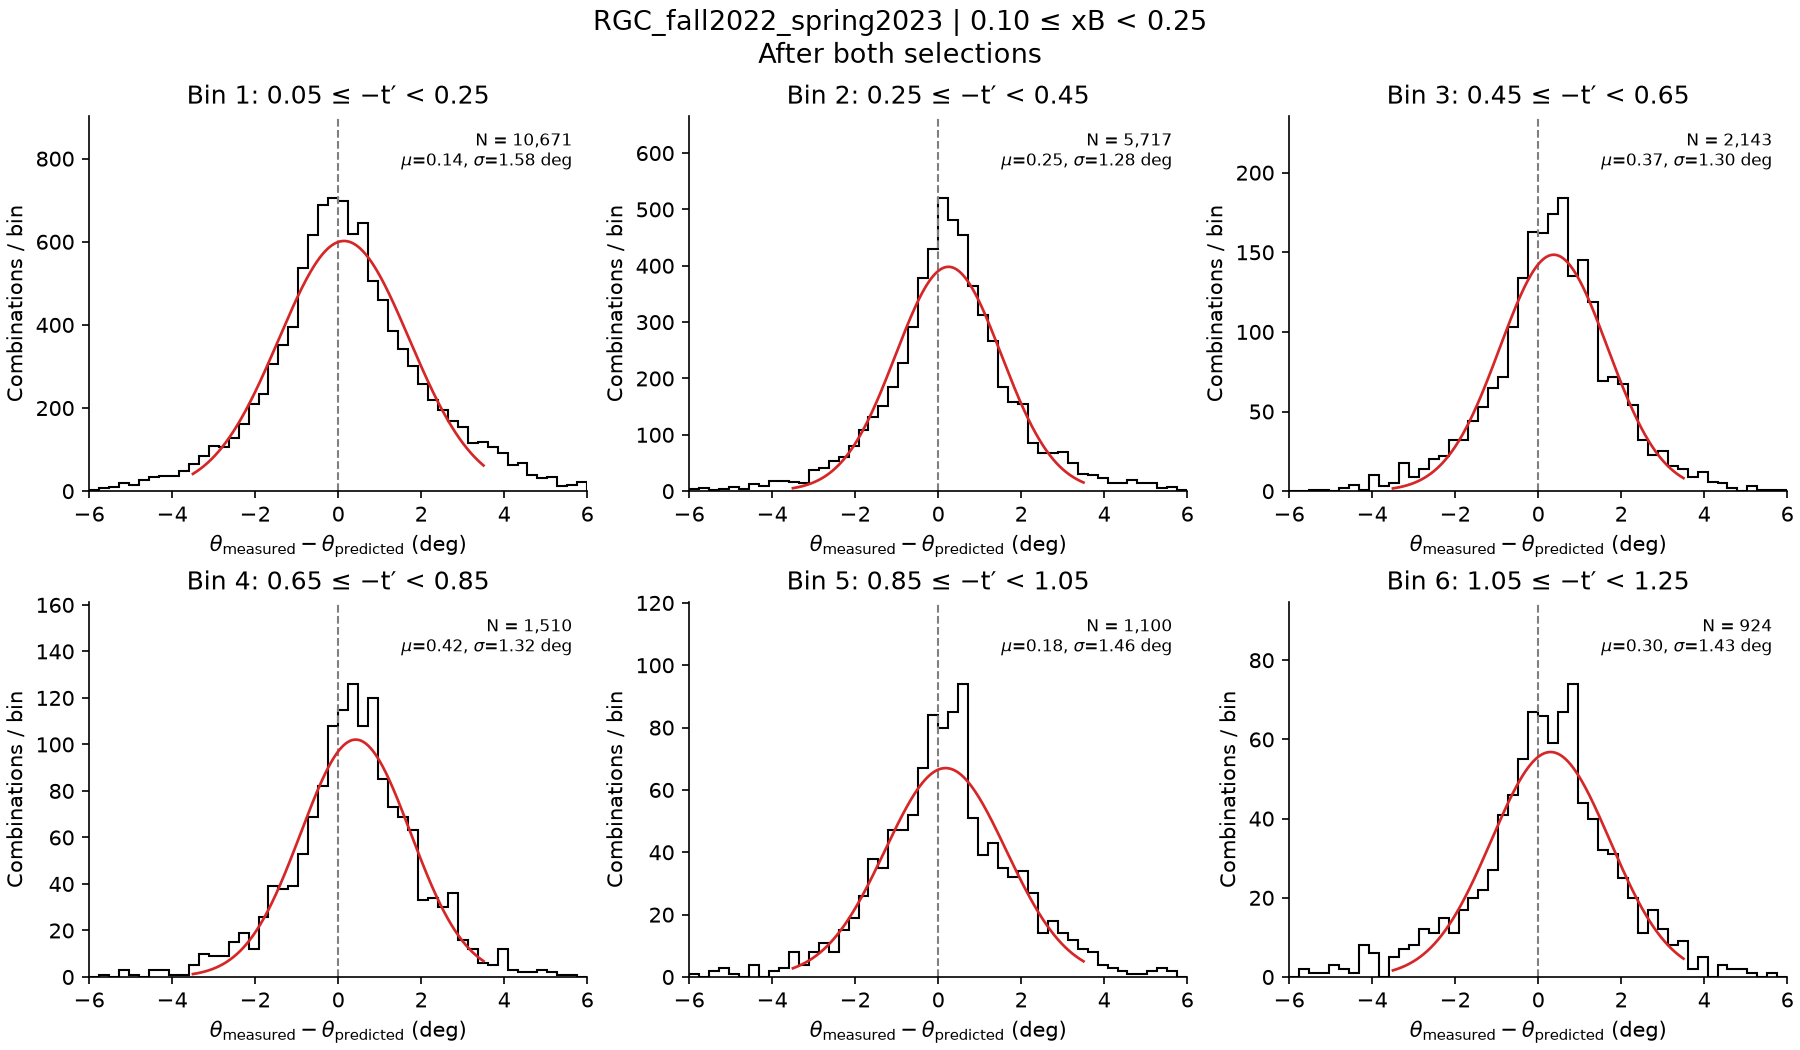
\includegraphics[width=\linewidth]{figures/channel_selection/exclusivity/rgc_fa22_sp23_angle_xb1.png}
\caption{RGC\_fall2022\_spring2023: pion polar-angle closure after both cuts in $x_B$ interval 1. The panels retain the six fine selection bins.}\label{fig:new_excl_rgc_fa22_sp23_angle1}
\end{figure}
\clearpage
\begin{figure}[p]\centering
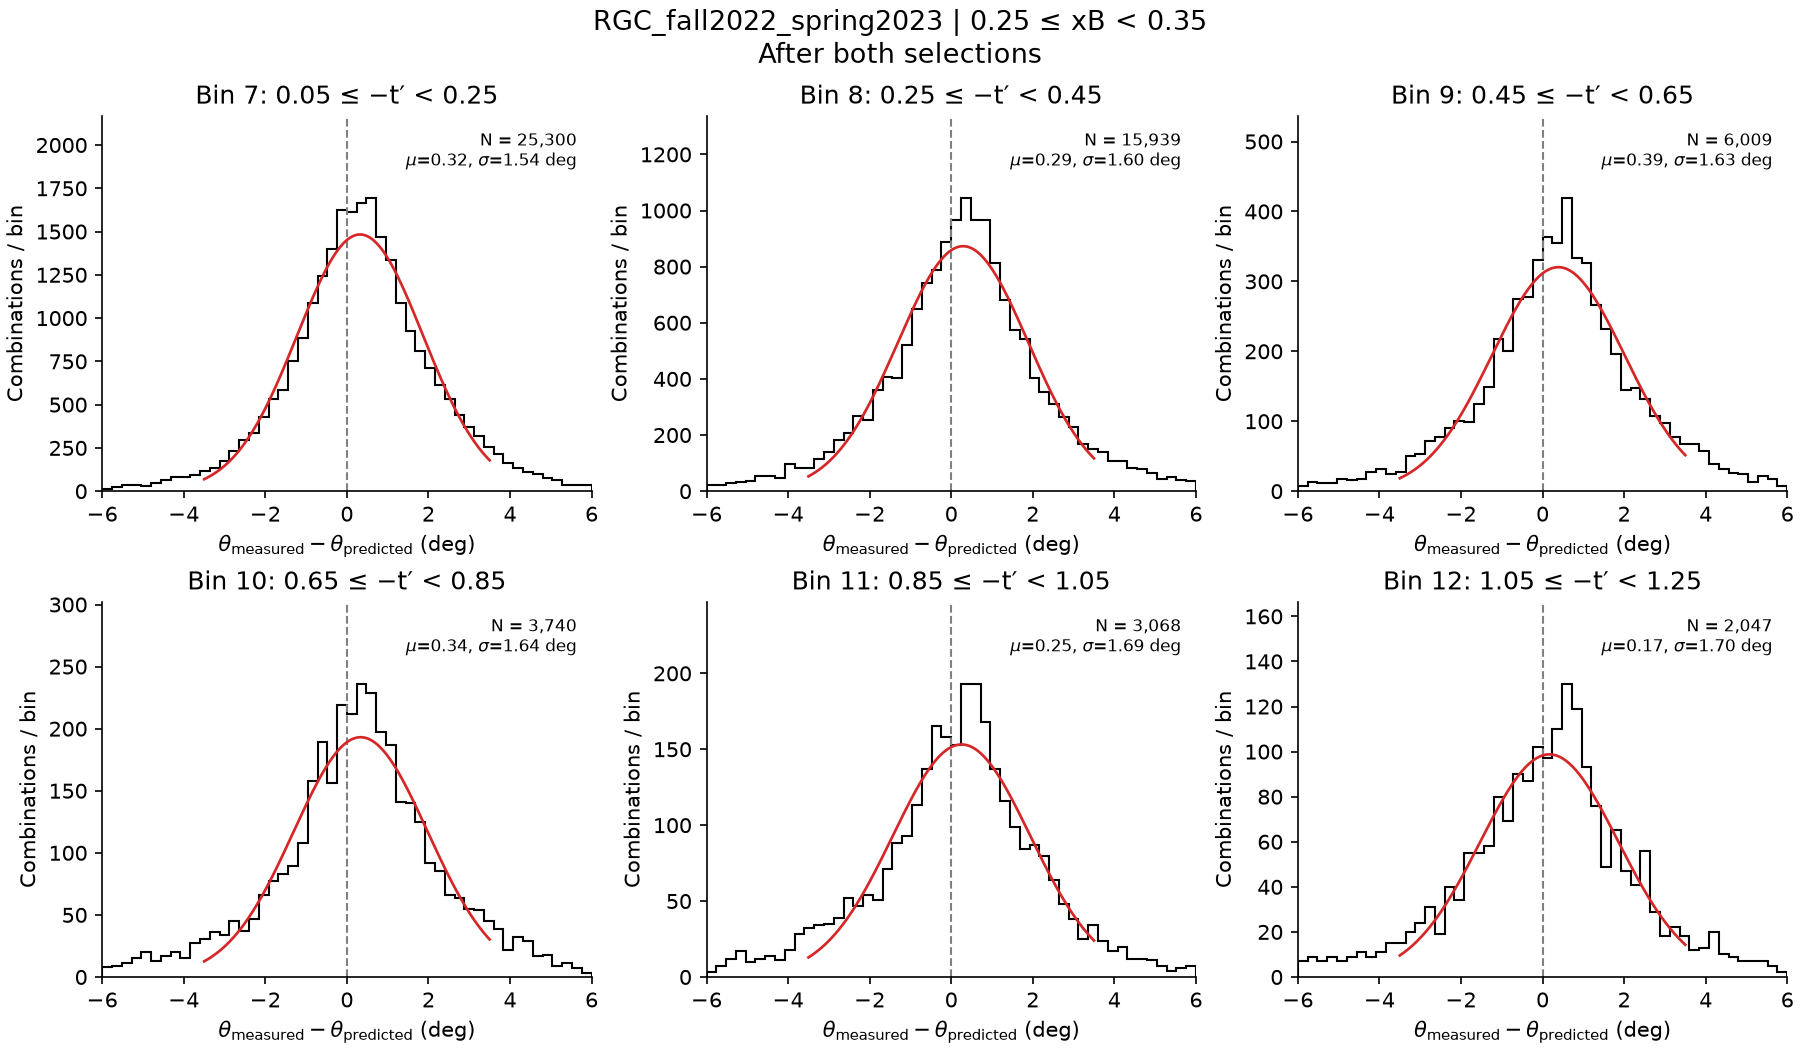
\includegraphics[width=\linewidth]{figures/channel_selection/exclusivity/rgc_fa22_sp23_angle_xb2.png}
\caption{RGC\_fall2022\_spring2023: pion polar-angle closure after both cuts in $x_B$ interval 2. The panels retain the six fine selection bins.}\label{fig:new_excl_rgc_fa22_sp23_angle2}
\end{figure}
\clearpage
\begin{figure}[p]\centering
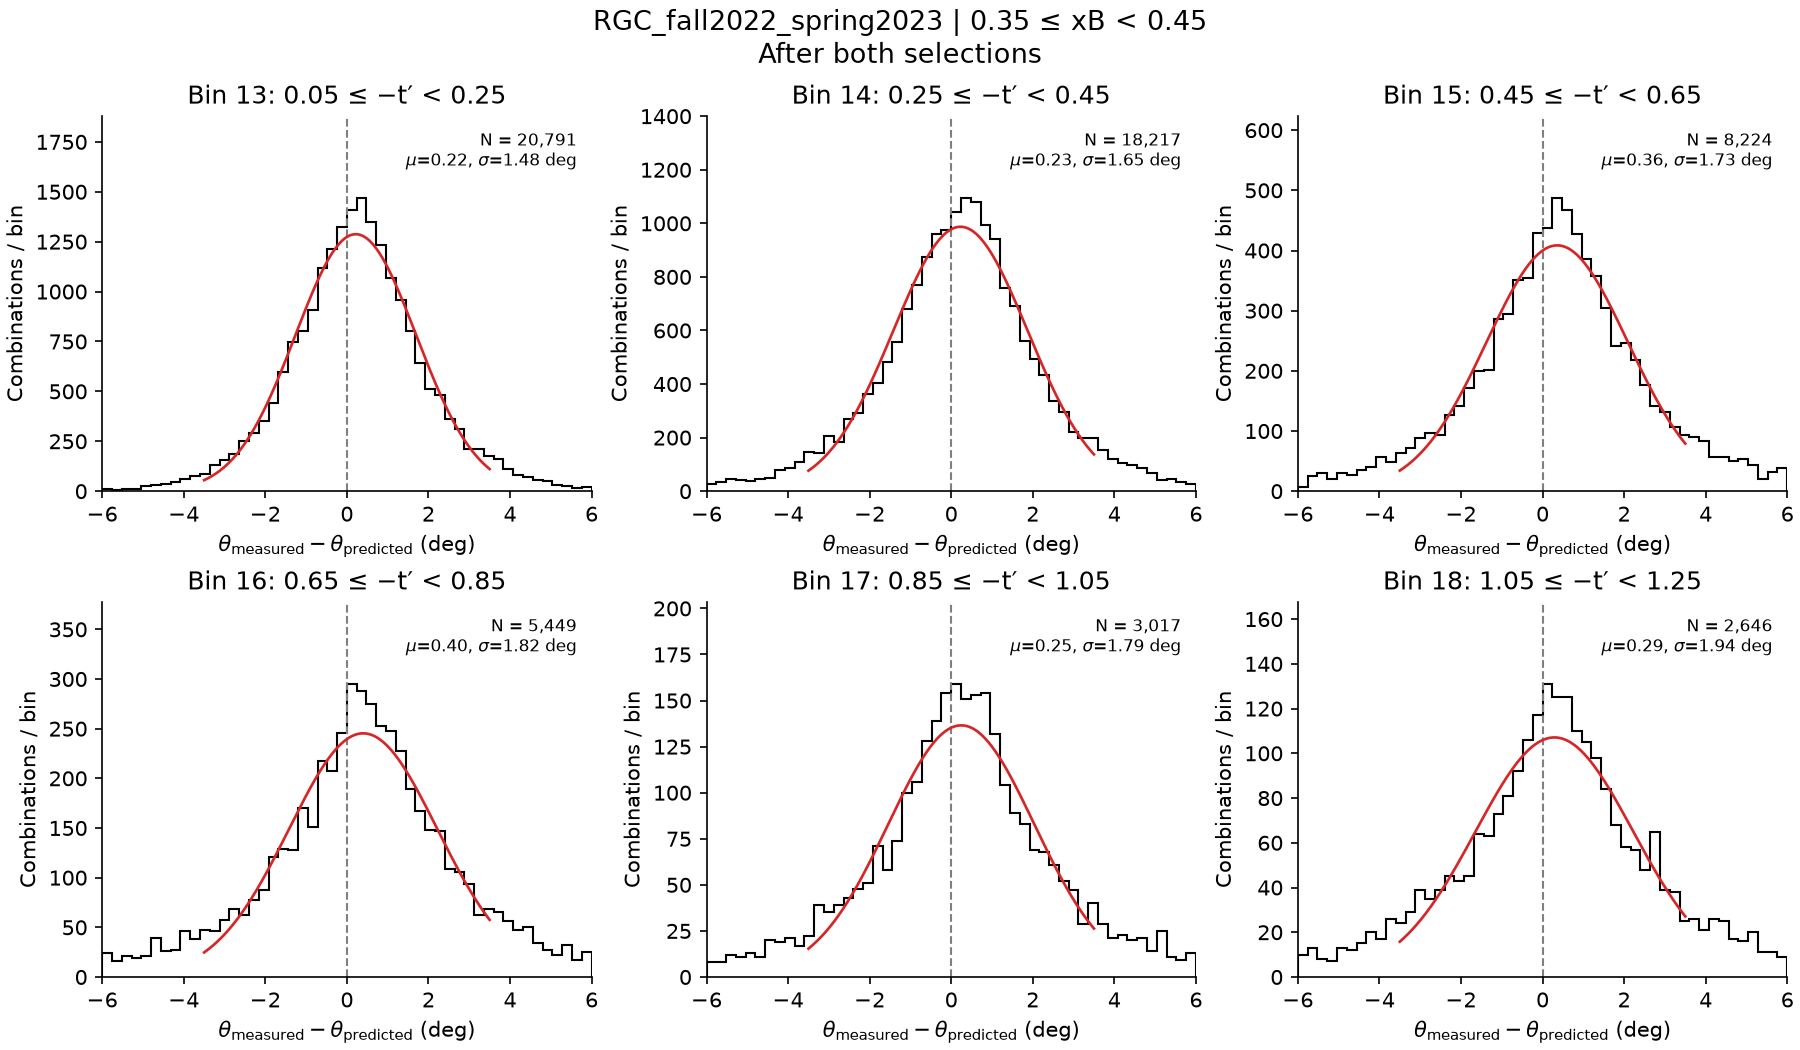
\includegraphics[width=\linewidth]{figures/channel_selection/exclusivity/rgc_fa22_sp23_angle_xb3.png}
\caption{RGC\_fall2022\_spring2023: pion polar-angle closure after both cuts in $x_B$ interval 3. The panels retain the six fine selection bins.}\label{fig:new_excl_rgc_fa22_sp23_angle3}
\end{figure}
\clearpage
\begin{figure}[p]\centering
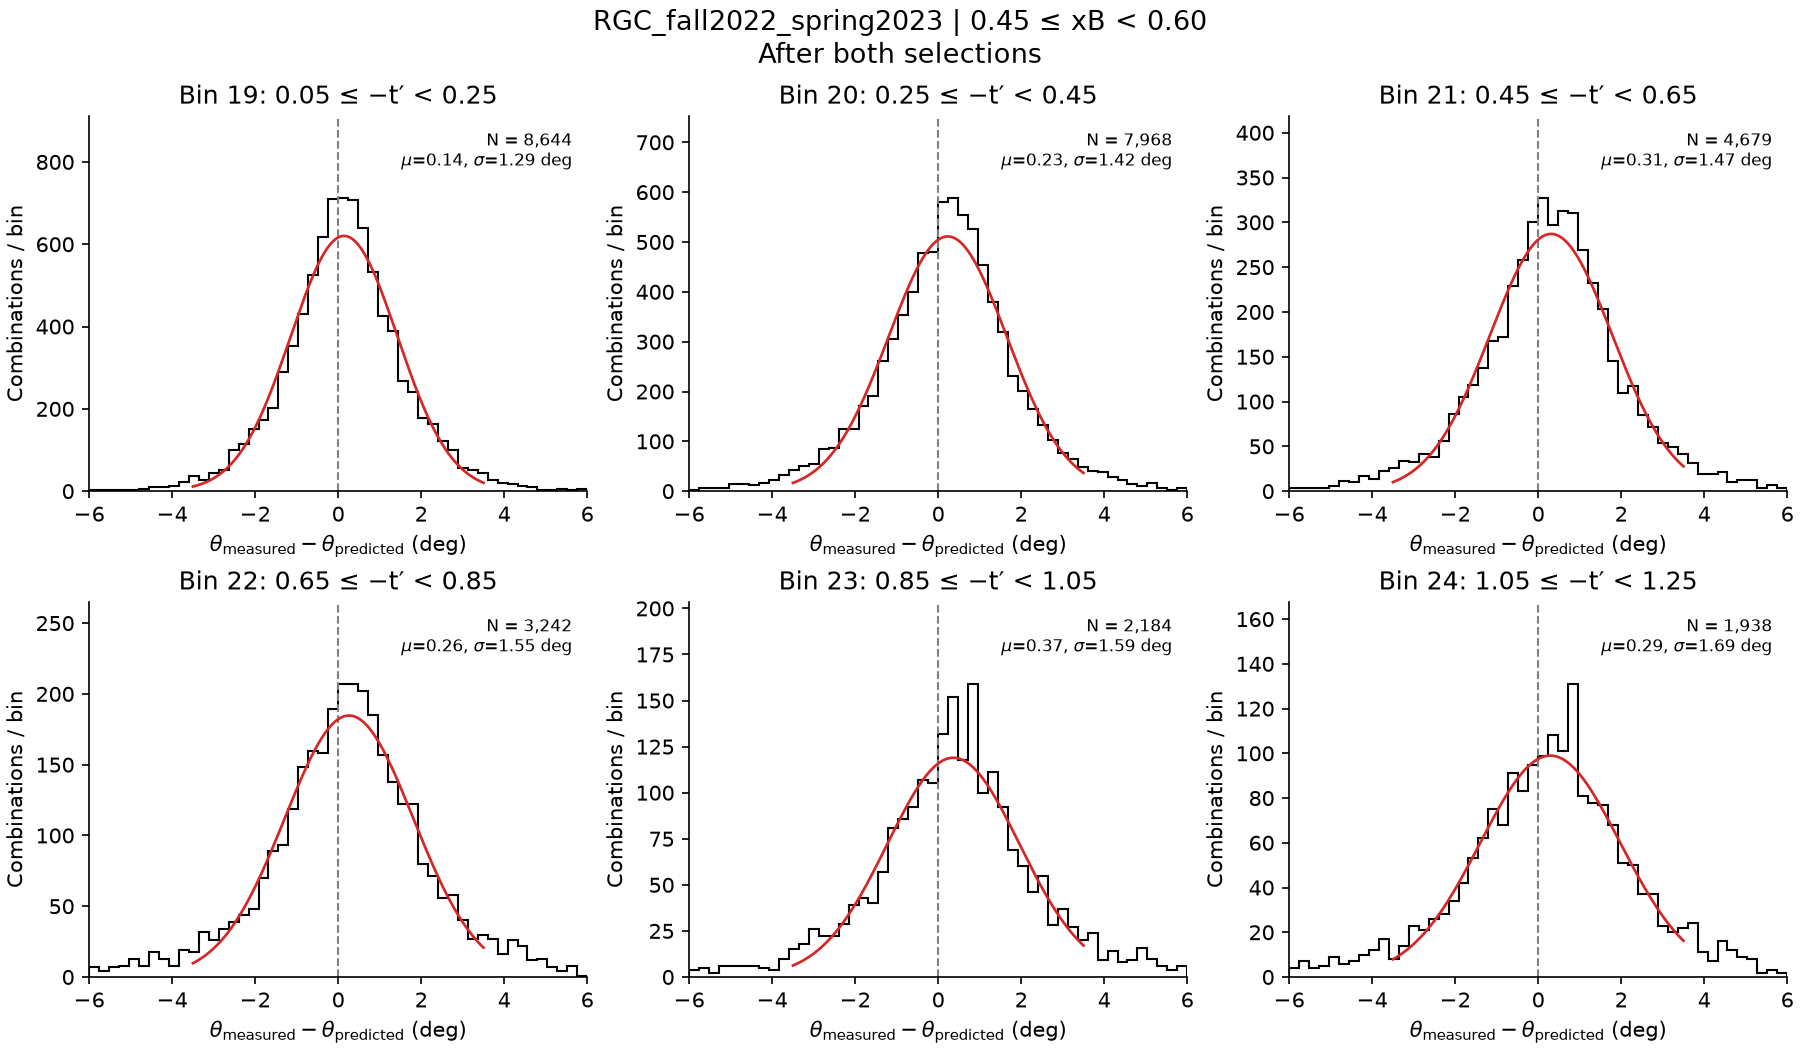
\includegraphics[width=\linewidth]{figures/channel_selection/exclusivity/rgc_fa22_sp23_angle_xb4.png}
\caption{RGC\_fall2022\_spring2023: pion polar-angle closure after both cuts in $x_B$ interval 4. The panels retain the six fine selection bins.}\label{fig:new_excl_rgc_fa22_sp23_angle4}
\end{figure}
\clearpage


\clearpage\section{Asymmetry Extraction}
\subsection{Binning}\label{sec:release_binning}
The four $x_B$ intervals are $[0.10,0.25)$, $[0.25,0.35)$, $[0.35,0.45)$ and $[0.45,0.60)$. The event selection and exclusivity calibration retain six $-t'$ intervals per $x_B$: $[0.05,0.25)$, $[0.25,0.45)$, $[0.45,0.65)$, $[0.65,0.85)$, $[0.85,1.05)$ and $[1.05,1.25)$ GeV$^2$. Bin numbers increase through $-t'$ first and then $x_B$.
The beam-spin result retains these 24 bins. For the two target-spin results, adjacent pairs of selected bins are merged into $[0.05,0.45)$, $[0.45,0.85)$ and $[0.85,1.25)$ GeV$^2$, yielding 12 bins. The target-sector likelihood is refitted to the merged events and the dilution factor is recalculated from summed control-target counts, rather than averaging fitted ratios or corrections. Original fine-bin exclusivity windows remain attached to each event. Points are displayed at the selected combined-sample mean $-t'$ in their respective bins.

\clearpage
\begin{longtable}{lrrrrr}
\caption{Measured combined-sample kinematic means in the reported bins. The two $UL$ ratios share the same twelve-bin means.}\\
\toprule Observable & Bin & $\langle x_B\rangle$ & $\langle Q^2\rangle$ & $\langle W\rangle$ & $\langle-t^\prime\rangle$\\\midrule\endhead
$LU$ & 1 & 0.207 & 1.869 & 2.855 & 0.156\\
$LU$ & 2 & 0.203 & 1.924 & 2.927 & 0.332\\
$LU$ & 3 & 0.203 & 1.943 & 2.938 & 0.541\\
$LU$ & 4 & 0.201 & 1.929 & 2.944 & 0.745\\
$LU$ & 5 & 0.200 & 1.939 & 2.956 & 0.947\\
$LU$ & 6 & 0.201 & 1.953 & 2.962 & 1.146\\
$LU$ & 7 & 0.303 & 2.146 & 2.408 & 0.157\\
$LU$ & 8 & 0.306 & 2.209 & 2.422 & 0.333\\
$LU$ & 9 & 0.306 & 2.215 & 2.424 & 0.540\\
$LU$ & 10 & 0.305 & 2.244 & 2.439 & 0.743\\
$LU$ & 11 & 0.305 & 2.249 & 2.444 & 0.945\\
$LU$ & 12 & 0.304 & 2.275 & 2.456 & 1.146\\
$LU$ & 13 & 0.393 & 2.743 & 2.250 & 0.158\\
$LU$ & 14 & 0.394 & 2.790 & 2.261 & 0.338\\
$LU$ & 15 & 0.396 & 2.826 & 2.264 & 0.539\\
$LU$ & 16 & 0.396 & 2.845 & 2.270 & 0.743\\
$LU$ & 17 & 0.396 & 2.845 & 2.269 & 0.945\\
$LU$ & 18 & 0.397 & 2.857 & 2.272 & 1.146\\
$LU$ & 19 & 0.498 & 3.980 & 2.197 & 0.156\\
$LU$ & 20 & 0.499 & 4.045 & 2.206 & 0.343\\
$LU$ & 21 & 0.503 & 4.109 & 2.206 & 0.543\\
$LU$ & 22 & 0.506 & 4.169 & 2.210 & 0.744\\
$LU$ & 23 & 0.507 & 4.189 & 2.210 & 0.946\\
$LU$ & 24 & 0.506 & 4.158 & 2.205 & 1.146\\
$UL$ & 1 & 0.205 & 1.887 & 2.878 & 0.214\\
$UL$ & 2 & 0.202 & 1.937 & 2.940 & 0.626\\
$UL$ & 3 & 0.201 & 1.945 & 2.958 & 1.034\\
$UL$ & 4 & 0.304 & 2.168 & 2.412 & 0.216\\
$UL$ & 5 & 0.305 & 2.225 & 2.429 & 0.611\\
$UL$ & 6 & 0.305 & 2.260 & 2.449 & 1.032\\
$UL$ & 7 & 0.393 & 2.762 & 2.255 & 0.232\\
$UL$ & 8 & 0.396 & 2.833 & 2.266 & 0.613\\
$UL$ & 9 & 0.396 & 2.850 & 2.271 & 1.034\\
$UL$ & 10 & 0.499 & 4.010 & 2.201 & 0.241\\
$UL$ & 11 & 0.504 & 4.132 & 2.207 & 0.618\\
$UL$ & 12 & 0.506 & 4.175 & 2.208 & 1.034\\
\bottomrule\end{longtable}


\subsection{Beam and Target Polarizations}
\label{sec::polarization}
The beam polarization is determined through a series of M\"{o}ller measurements taken throughout the data taking period. The various M\"{o}ller runs and their associated logbook entries are all included in the supplemental document \href{https://clas12-docdb.jlab.org/DocDB/0012/001257/001/rgc_beam_polarizations.txt}{RGC Beam Polarizations}. The final beam polarization percentages are RGC Su22: 83.84 +/- 0.86(stat) +/- 2.16(sys), RGC Fa22: 83.72 +/- 0.45(stat) +/- 2.91(sys) and RGC Sp23: 80.40 +/- 0.61(stat) +/- 4.70(sys). The bulk of the systematic uncertainty comes from an absolute scale uncertainty in the M\"{o}ller measurements that is estimated at about 2\% with the remaining coming from measurement-to-measurement variance.

The nominal ND$_3$ target polarization is obtained from the elastic-scattering determination of $P_bP_t$ and the measured beam polarization,
\begin{equation}\label{eq:target_polarization}
P_t=\frac{P_bP_t}{P_b}.
\end{equation}
The preliminary elastic results from the \href{https://clasweb.jlab.org/wiki/index.php/Elastic_Analysis_for_PbPt_Extraction}{RGC elastic-polarization analysis} and the corresponding target polarizations are listed in Table~\ref{tab:pt_by_period}.
\begin{table}[H]\centering\small
\begin{tabular}{llrr}\toprule Period & target sign & elastic $P_bP_t$ & derived $P_t$\\\midrule
Su22 & + & $0.20\pm0.03$ & $0.2385\pm0.0364$ \\
Su22 & - & $-0.14\pm0.04$ & $-0.1670\pm0.0479$ \\
Fa22 & + & $0.23\pm0.02$ & $0.2747\pm0.0258$ \\
Fa22 & - & $-0.25\pm0.02$ & $-0.2986\pm0.0261$ \\
Sp23 & + & $0.26\pm0.03$ & $0.3234\pm0.0419$ \\
Sp23 & - & $-0.14\pm0.03$ & $-0.1741\pm0.0387$ \\
\bottomrule\end{tabular}
\caption{Preliminary elastic beam--target products and derived ND$_3$ target polarizations. Product errors are the quoted elastic statistical uncertainties. The target-polarization errors propagate the elastic statistical uncertainty and the M\"{o}ller statistical and systematic uncertainties.}\label{tab:pt_by_period}\end{table}

A comparison with the independent \href{https://clasweb.jlab.org/wiki/index.php/DIS_Analysis_for_PbPt_Extraction}{DIS determination of $P_bP_t$} is ongoing. The preliminary results use the elastic determination. A combined polarization scale uncertainty is not quoted for this preliminary analysis.

The RGB liquid-D$_2$ target is unpolarized, so $P_t=0$ for all RGB periods. The RGB beam polarization remains nonzero and enters the beam-spin terms in the likelihood.

\subsection{Dilution Factor Calculation}
\label{sec::df}
In the longitudinally polarized deuterated-ammonia (ND$_3$) target, the selected events include contributions from deuterium, nitrogen, helium coolant and target-cell material. It is therefore necessary to determine the fraction originating from deuterium. This fraction is referred to as the dilution factor, $D_f$. The RGC dilution-factor formalism is described in the standalone document ``\href{https://clasweb.jlab.org/wiki/images/7/72/Dilution_Factor_Determination_for_RG_C_10-16-26.pdf}{Dilution Factor Determination for RG-C}'' by S.~E.~Kuhn, D.~Holmberg and D.~W.~Upton. We calculate $D_f$ directly from charge-normalized ND$_3$, C, CD$_2$, He-bath and empty-target measurements, using Eq.~7 and the ND$_3$ coefficients in Table~II of that document.

The auxiliary-target measurements separate the carbon-like nuclear contribution, helium and cell material from the deuterium contribution. The calculation also accounts for the helium displaced by the solid targets. All samples receive the same exclusivity cuts as the ND$_3$ data from their run period. With $n_T=N_T/Q_T$, the thermally corrected expression is
\begin{align}
S &= n_{\mathrm{CD}_2}-0.765506n_C-0.000757116n_{\mathrm{He}}-0.233737n_{\mathrm{ET}},\\
D &= n_{\mathrm{CD}_2}-0.170112n_C-0.863533n_{\mathrm{He}}+0.0336457n_{\mathrm{ET}},\\
D_f &= \frac{(n_{\mathrm{ND}_3}-n_{\mathrm{He}})S}{n_{\mathrm{ND}_3}D}.
\end{align}
CD$_2$ was measured only in Sp23. For Su22 and Fa22 we multiply the charge-normalized CH$_2$ yield by the Sp23 CD$_2$/CH$_2$ ratio, determined in the same kinematic bin. Figure~\ref{fig:df_controls} compares the measured Sp23 distributions.

\begin{figure}[htbp]\centering
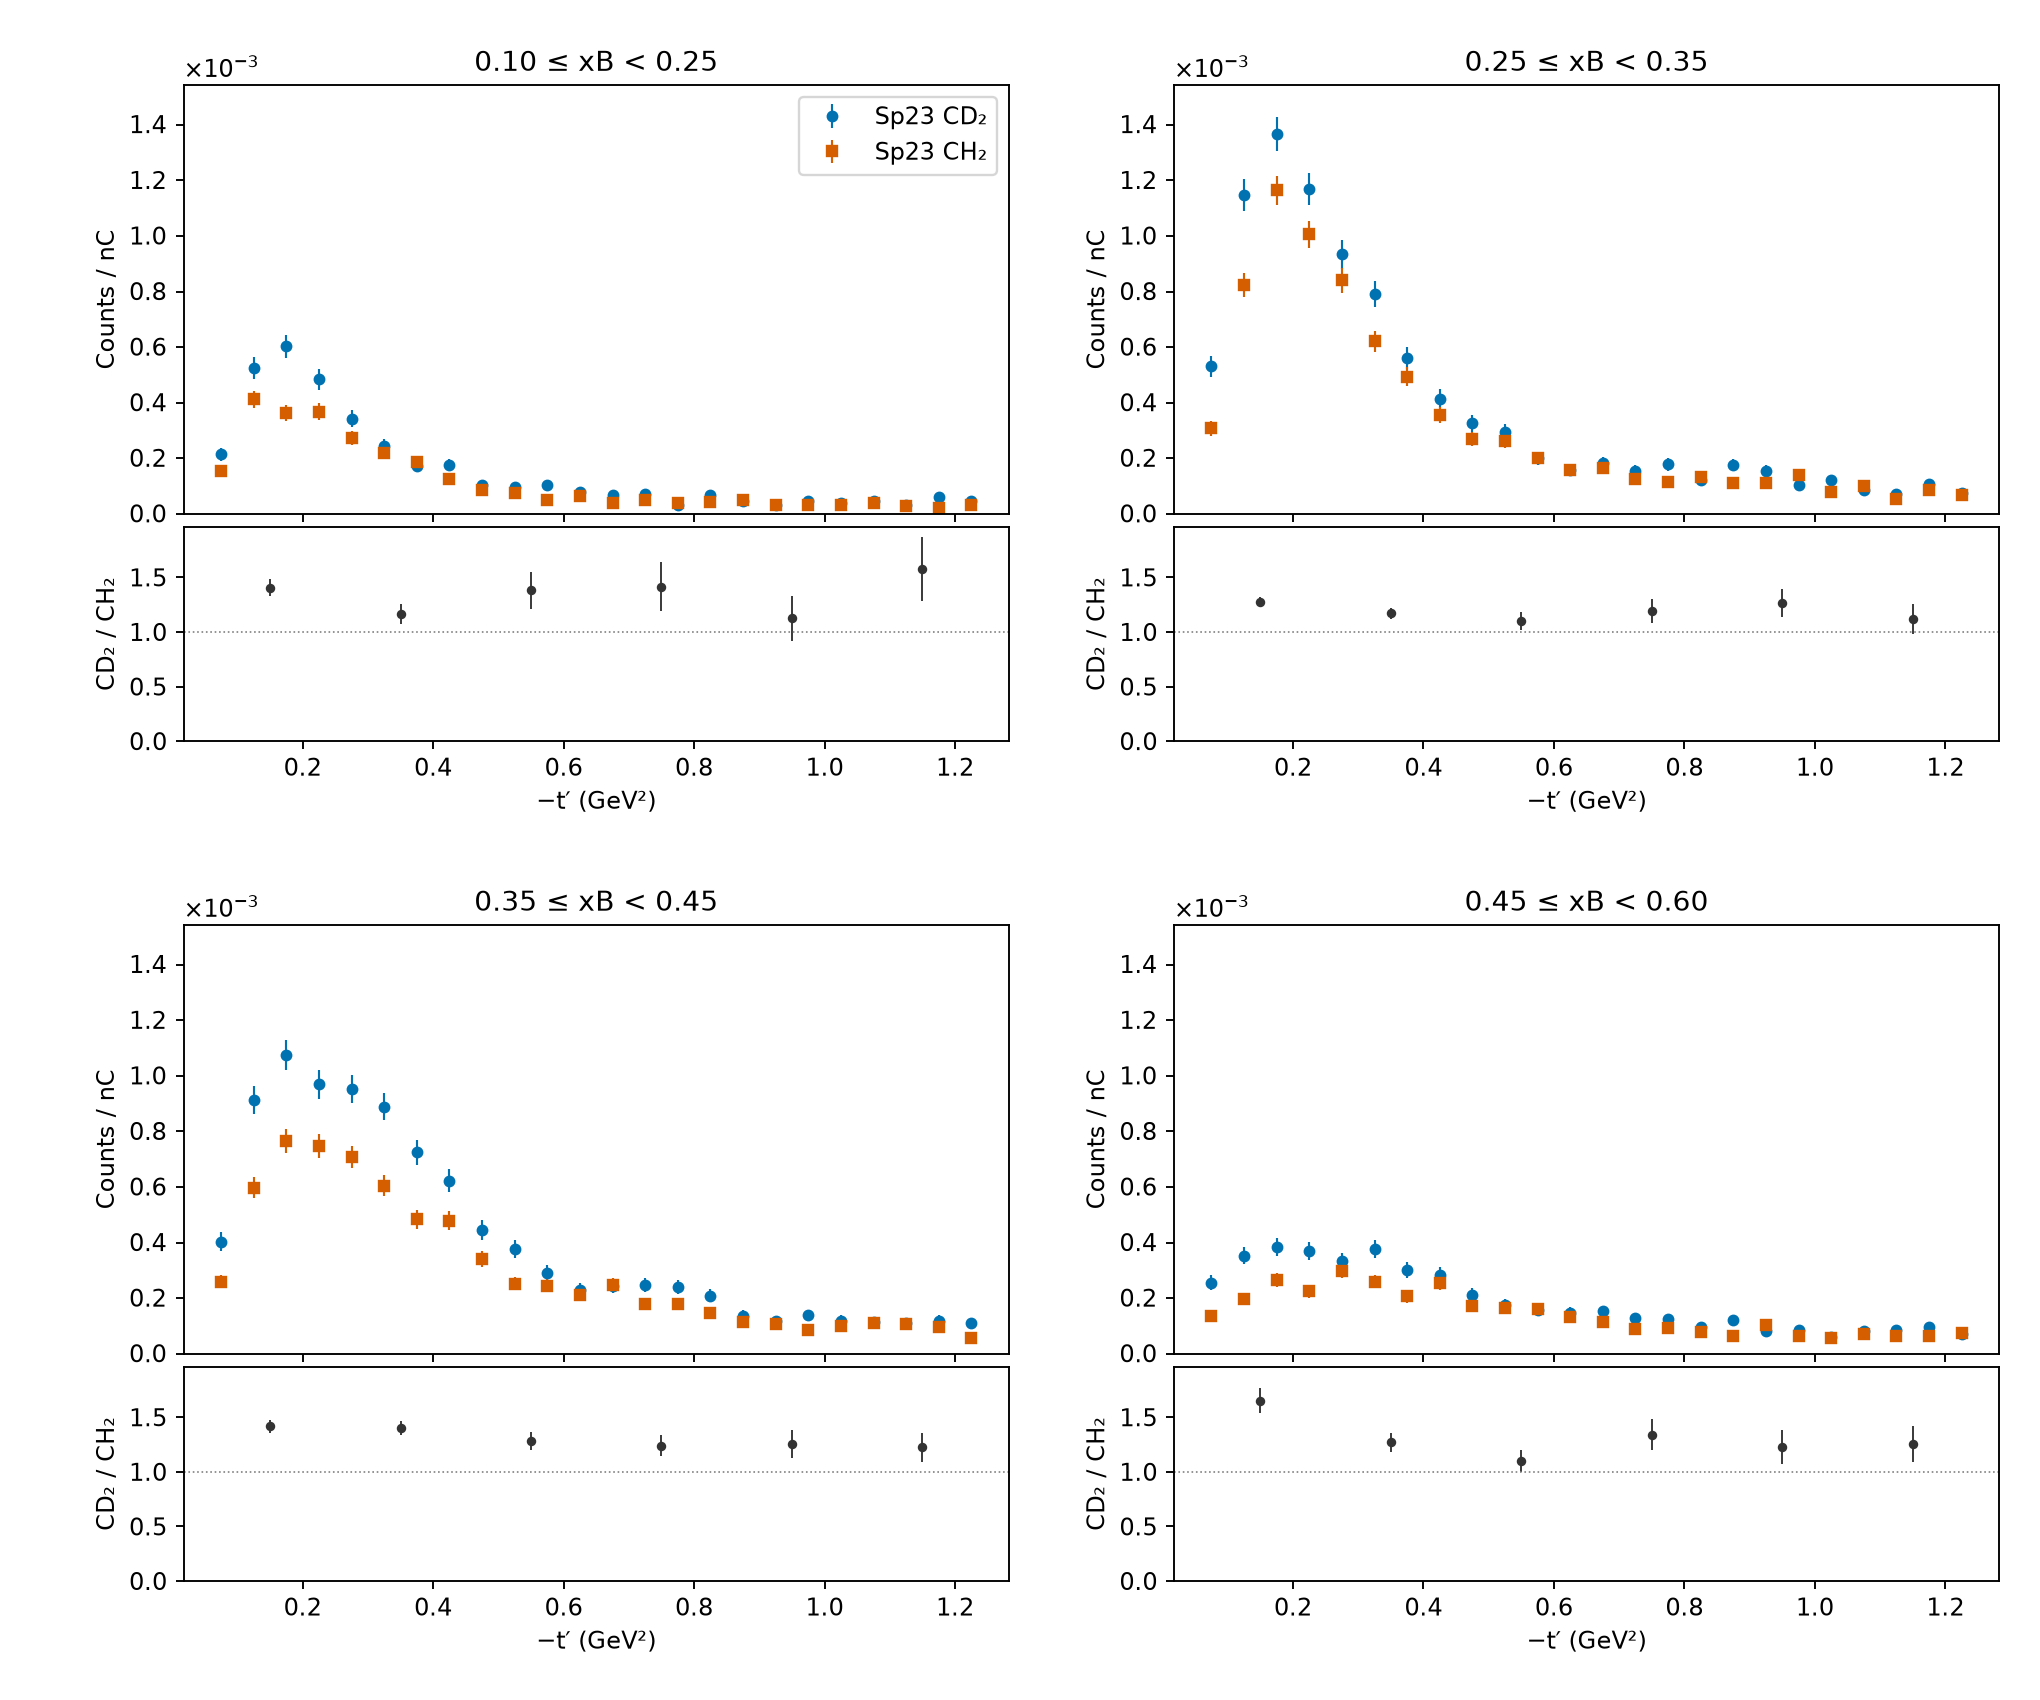
\includegraphics[width=\linewidth]{figures/asymmetry_extraction/dilution_factor/cd2_ch2_distributions.png}
\caption{Sp23 CD$_2$ and CH$_2$ yields normalized to charge, with their ratios below. The ratio panels use the six analysis bins in $-t'$.}\label{fig:df_controls}
\end{figure}

We first compare the three periods after integrating over either $-t'$ or $x_B$ (Fig.~\ref{fig:df_periods}). Correlated statistical comparisons give $\chi^2/\mathrm{ndf}=9.73/8$ ($p=0.285$) for the $x_B$ dependence and $6.43/12$ ($p=0.893$) for the $-t'$ dependence. The comparisons include correlations from the shared Sp23 measurements.

\begin{figure}[htbp]\centering
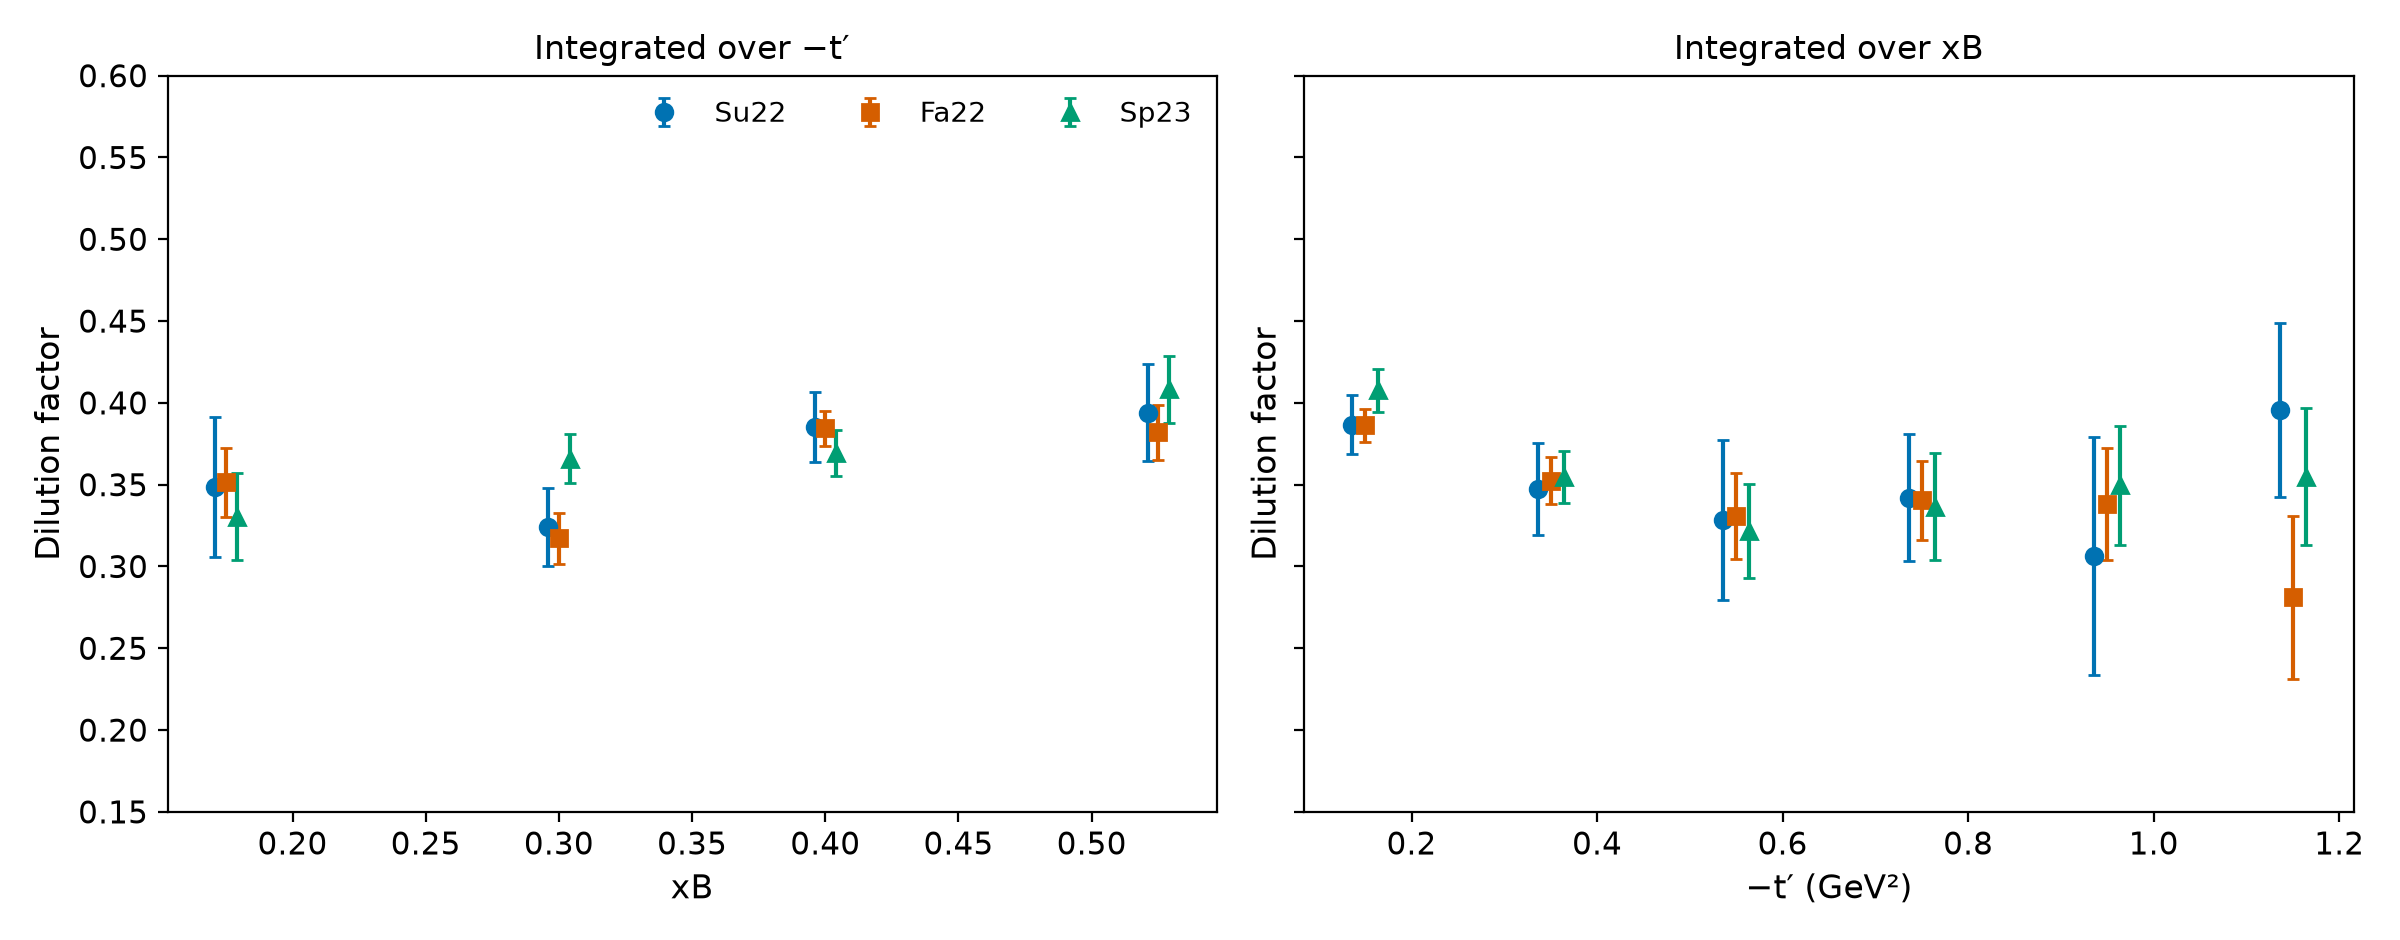
\includegraphics[width=\linewidth]{figures/asymmetry_extraction/dilution_factor/period_agreement.png}
\caption{Period comparisons integrated over $-t'$ (left) or $x_B$ (right). Error bars show statistical standard deviations from Poisson replicas. Points are slightly displaced horizontally for readability.}\label{fig:df_periods}
\end{figure}

For the released target-spin ratios, adjacent fine bins are merged before the material calculation. A shared-period dilution factor is fitted in each of the twelve merged bins, retaining independent period target rates and the common Sp23 CD$_2$/CH$_2$ transfer. Statistical errors are the standard deviations of 2,000 independent Poisson-replica fits per bin. The $LU$ ratio receives no direct dilution correction. The earlier 24-bin corrections remain available as a cross-check but are not used for the released three-bin $UL$ ratios.
\clearpage
\begin{longtable}{rrrr}
\caption{Shared-period dilution factors in the twelve target-sector bins.}\\
\toprule Bin & $D_f$ & Statistical error & Joint deviance\\\midrule\endhead
1 & 0.3346 & 0.0239 & 0.74\\
2 & 0.3915 & 0.0476 & 5.42\\
3 & 0.3108 & 0.0632 & 2.06\\
4 & 0.3423 & 0.0126 & 6.53\\
5 & 0.3233 & 0.0277 & 4.47\\
6 & 0.3230 & 0.0381 & 0.02\\
7 & 0.4000 & 0.0102 & 1.21\\
8 & 0.3433 & 0.0247 & 1.09\\
9 & 0.3282 & 0.0351 & 1.46\\
10 & 0.4378 & 0.0141 & 3.54\\
11 & 0.3107 & 0.0409 & 0.15\\
12 & 0.3367 & 0.0461 & 0.66\\
\bottomrule\end{longtable}

\begin{figure}[p]\centering
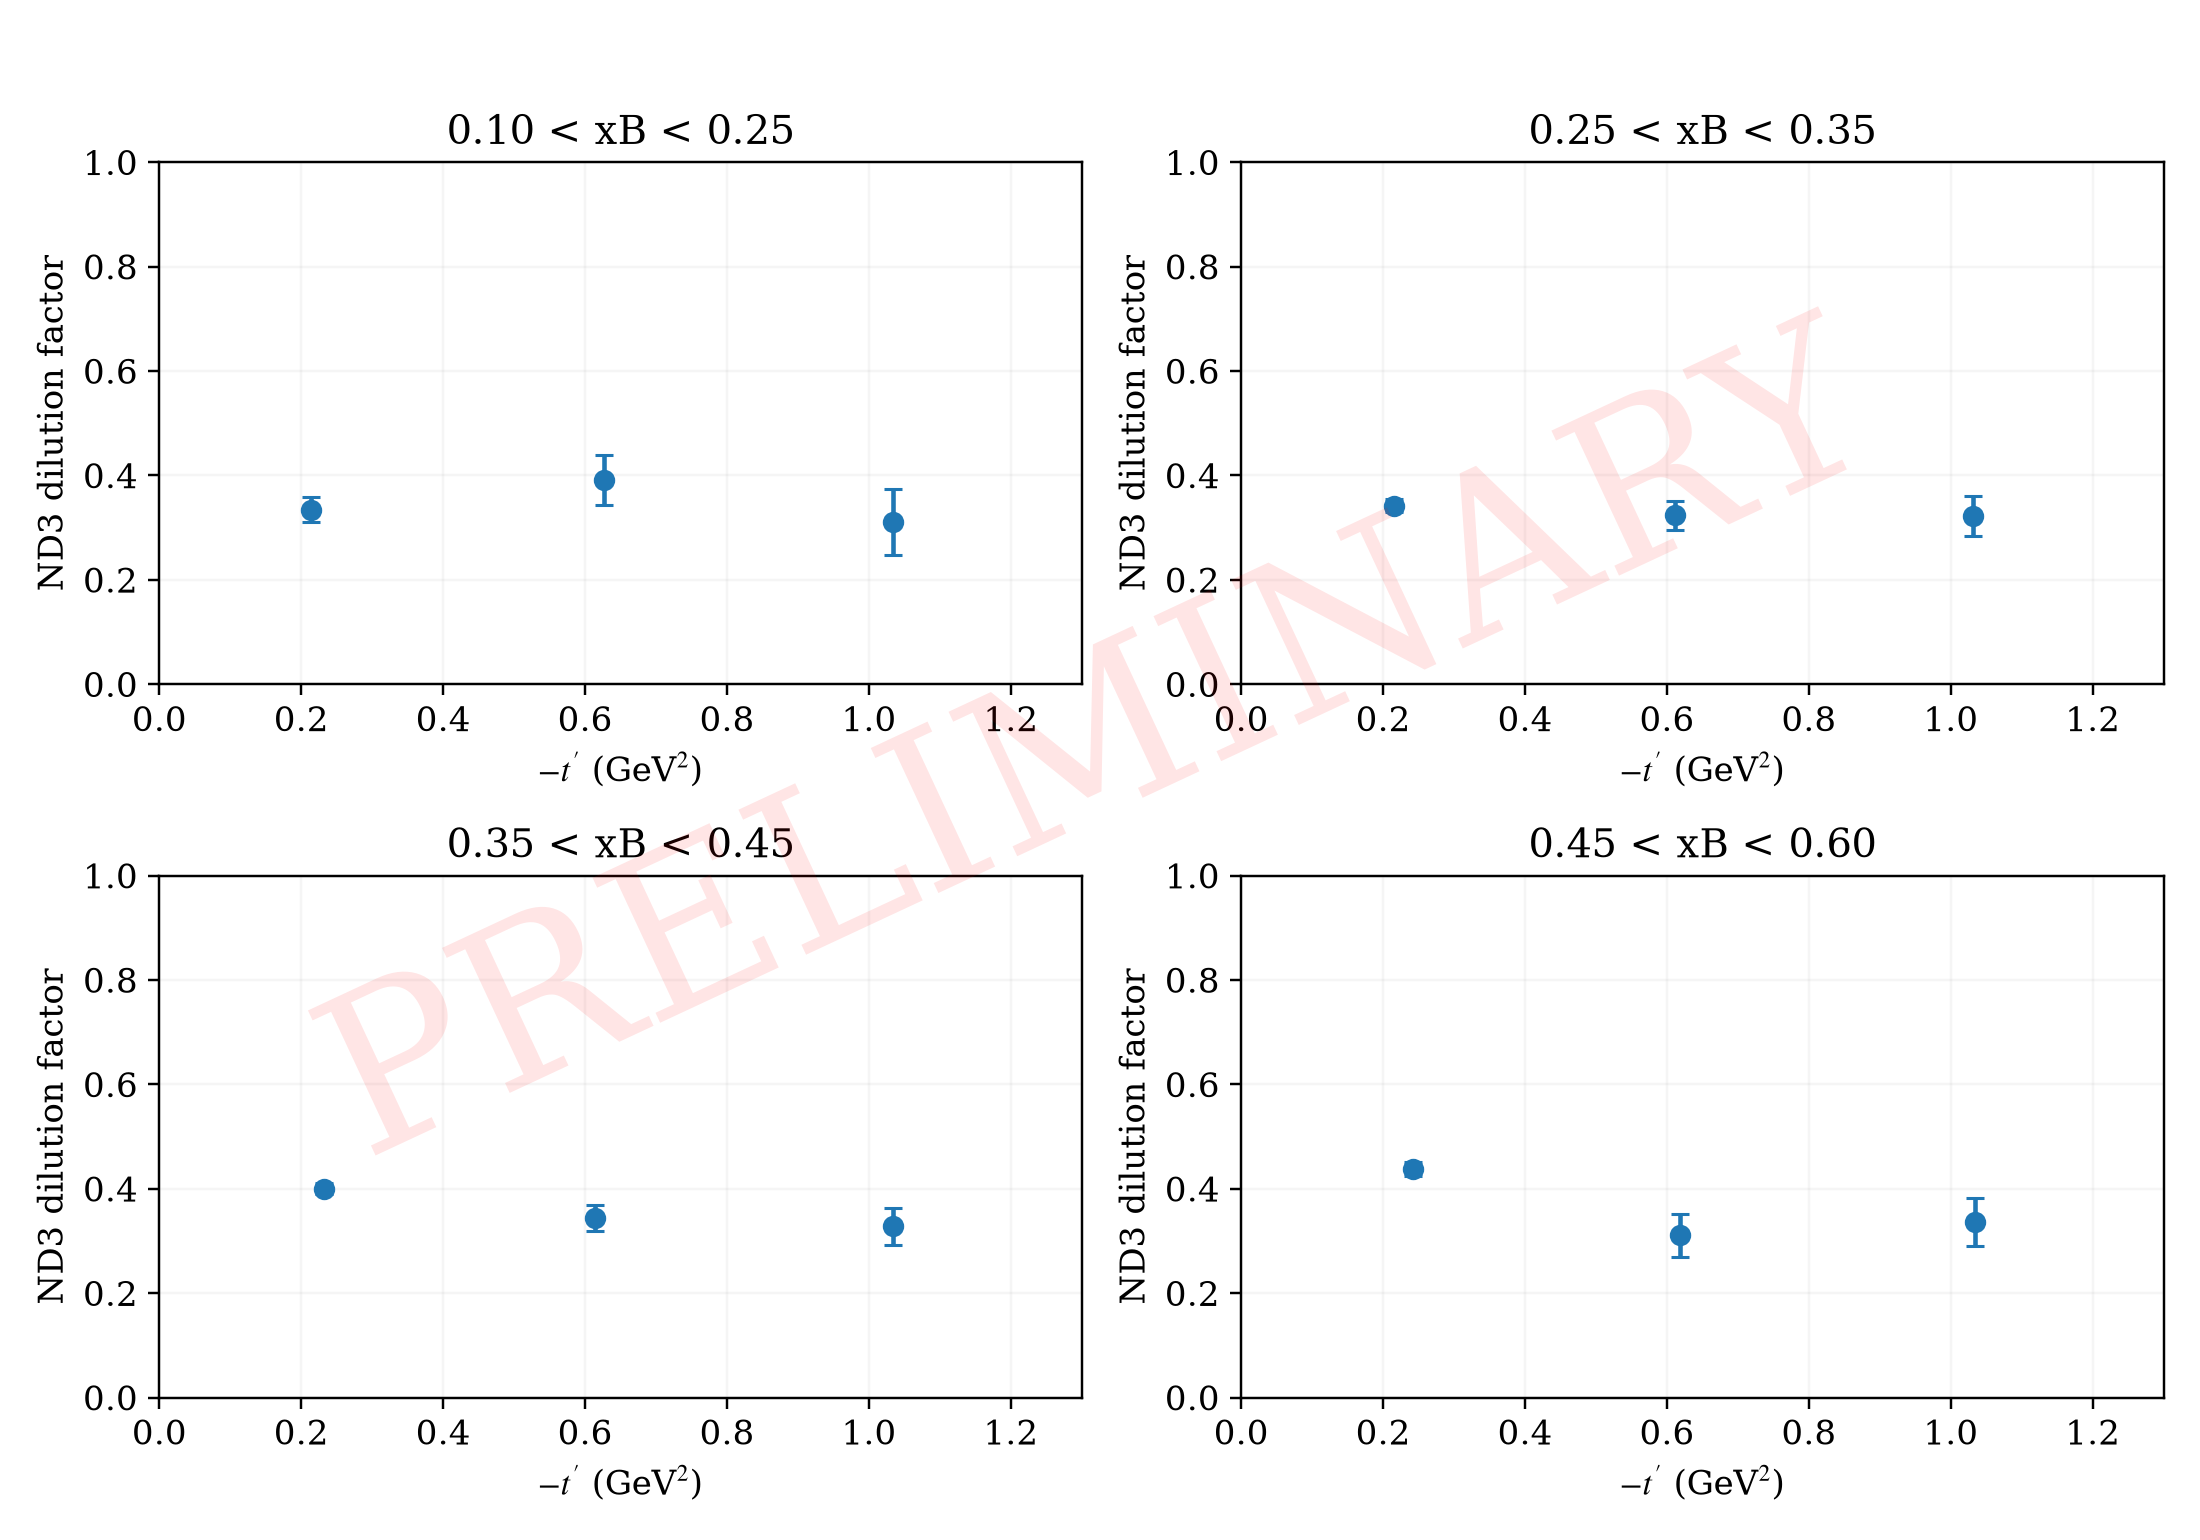
\includegraphics[width=\linewidth]{figures/results/dilution_12_bins.png}
\caption{Shared-period dilution factors in the twelve target-sector bins. Errors are the standard deviations from 2,000 Poisson-replica fits.}\label{fig:release_dilution}
\end{figure}
\clearpage

\subsection{Depolarization Factors}\label{sec:depolarization_factors}

The pure QED kinematic factors required to transform from the measured asymmetry values to the ratio of structure functions are the twist-2 functions $A$, $B$ and $C$ and the twist-3 functions $V$ and $W$ that are given by
\begin{align}
A(\epsilon, y) &\equiv \frac{y^2}{2(1-\epsilon)} = \frac{1}{1+\gamma^2} \left(1-y+\frac{1}{2}y^2 + \frac{1}{4}\gamma^2 y^2\right) \approx \left(1-y+\frac{1}{2} y^2 \right),\\
B(\epsilon, y) &\equiv \frac{y^2}{2(1-\epsilon)} \epsilon = \frac{1}{1+\gamma^2} \left(1-y-\frac{1}{4} \gamma^2 y^2 \right) \approx \left(1-y\right) ,\\
C(\epsilon, y) &\equiv \frac{y^2}{2\left(1-\epsilon\right)} \sqrt{1-\epsilon^2} = \frac{y}{\sqrt{1+\gamma^2}} \left(1-\frac{1}{2}y\right) \approx y \left(1-\frac{1}{2} y \right) , \\
V(\epsilon, y) &\equiv \frac{y^2}{2\left(1-\epsilon \right)} \sqrt{2 \epsilon (1+\epsilon)} = \frac{2-y}{1+\gamma^2} \sqrt{1-y-\frac{1}{4}\gamma^2y^2} \approx \left(2-y\right) \sqrt{1-y}, \\
W(\epsilon, y) &\equiv \frac{y^2}{2\left(1 - \epsilon\right)} \sqrt{2\epsilon(1-\epsilon)} = \frac{y}{\sqrt{1+\gamma^2}} \sqrt{1-y-\frac{1}{4} \gamma^2 y^2 } \approx y \sqrt{1-y},
\end{align}
and dependent on the ratio $\epsilon$ of longitudinal and transverse photon flux \cite{Bacchetta:2006tn},
\begin{align}
\epsilon = \frac{1 - y - \frac{1}{4}\gamma^2 y^2 }{1-y+\frac{1}{2}y^2 + \frac{1}{4}\gamma^2 y^2}.
\label{eps}
\end{align}
For a target polarization defined along the virtual-photon direction, the conventional relationship between asymmetry amplitudes and structure-function ratios is
\begin{align}
    A_{LU}^{\sin\phi} &= \left( \frac{W}{A} \right) \left( \frac{F_{LU}^{\sin\phi}}{F_{UU}} \right),\\
    A_{UL}^{\sin\phi} &= \left( \frac{V}{A} \right) \left( \frac{F_{UL}^{\sin\phi}}{F_{UU}} \right),~~~
    A_{UL}^{\sin2\phi} = \left( \frac{B}{A} \right) \left( \frac{F_{UL}^{\sin2\phi}}{F_{UU}} \right),\\
    A_{LL}^{} &= \left( \frac{C}{A} \right) \left( \frac{F_{LL}^{}}{F_{UU}} \right),~~~~
    A_{LL}^{\cos\phi} = \left( \frac{W}{A} \right) \left( \frac{F_{LL}^{\cos\phi}}{F_{UU}} \right),\\
    A_{UU}^{\cos\phi} &= \left( \frac{V}{A} \right) \left( \frac{F_{UU}^{\cos\phi}}{F_{UU}} \right),~~~
    A_{UU}^{\cos2\phi} = \left( \frac{B}{A} \right) \left( \frac{F_{UU}^{\cos2\phi}}{F_{UU}} \right)
\end{align}
where the dependence on $\epsilon$ and $y$ in the depolarization factors is omitted for brevity.  These relations define the conventional virtual-photon-axis quantities used for theoretical interpretation.  The nominal RGC target-spin and double-spin measurements are instead reported for the laboratory beam axis and are denoted $\frac{F_{UL,\mathrm{lab}}^{\sin\phi}}{F_{UU}}$, $\frac{F_{UL,\mathrm{lab}}^{\sin2\phi}}{F_{UU}}$, $\frac{F_{LL,\mathrm{lab}}}{F_{UU}}$ and $\frac{F_{LL,\mathrm{lab}}^{\cos\phi}}{F_{UU}}$.  This notation is intentionally distinct from the virtual-photon-axis quantities $F_{UL}^{h}/F_{UU}$ and $F_{LL}^{h}/F_{UU}$ above.  The ``lab'' quantities retain the event-by-event depolarization factors in their definition and extraction; they are not obtained by first forming a raw asymmetry and subsequently applying a bin-averaged depolarization correction. The extraction retains event-level factors throughout. No replacement by bin-averaged factors is made.


\subsection{Probability Density Function}
\label{sec:pdf}

The RGC ND$_3$ and RGB D$_2$ samples are described by a common set of azimuthal amplitudes. For a period $p$, the differential yield is written as
\begin{linenomath}
\begin{equation}
\label{eq:pdf}
 dN_p(\vec{\theta},\vec{x},h_b,P_t)
 =L_p\,\eta_p(\vec{x})\,\bar{\sigma}_{UU,p}(\vec{x})
 \mathcal{G}_p(\vec{\theta},\vec{x},h_b,P_t).
\end{equation}
\end{linenomath}
Here $\vec{x}$ denotes the event kinematics, $\vec{\theta}$ contains the fitted structure-function ratios, $L_p$ is the luminosity, and $\eta_p$ is the detector acceptance folded with the efficiency. The quantity $\bar{\sigma}_{UU,p}$ is the unpolarized, $\phi$-independent cross section. The beam helicity is $h_b=\pm1$, $P_b$ is the beam-polarization magnitude, and $P_t$ is the signed target polarization. The acceptance may differ between periods and between RGB and RGC. Its cancellation within each period is discussed below.

The RGC target is polarized along the incident electron beam. We therefore define the measured target-spin and double-spin ratios with respect to this laboratory axis and denote them by the subscript ``lab''. The target polarization entering the fit is $P_t$, without an additional $\cos\theta_\gamma$ projection. The effect of choosing the target axis was studied in the exclusive $\pi^+$ analysis. For this preliminary $\pi^-$ analysis, we retain the laboratory-frame definition and do not import transverse-target amplitudes measured in the $\pi^+$ channel. Theoretical predictions should use the same target-spin orientation and harmonic definitions. Predictions expressed along the virtual-photon axis can be related to the measured laboratory-frame quantities by including the corresponding longitudinal and transverse target contributions at the measured angle $\theta_\gamma$.

Using the event-level depolarization ratios
\begin{linenomath}
\begin{equation}
 r_B=\frac{B}{A},\qquad r_C=\frac{C}{A},\qquad
 r_V=\frac{V}{A},\qquad r_W=\frac{W}{A},
\end{equation}
\end{linenomath}
the fitted cross-section factor is
\begin{linenomath}
\begin{align}
\label{eq:cross_section_factor}
\mathcal{G}_p={}&1
 +r_V\frac{F_{UU}^{\cos\phi}}{F_{UU}}\cos\phi
 +r_B\frac{F_{UU}^{\cos2\phi}}{F_{UU}}\cos2\phi
 +h_bP_b r_W\frac{F_{LU}^{\sin\phi}}{F_{UU}}\sin\phi
 \nonumber\\
 &+D_fP_t\left[
 r_V\frac{F_{UL,\mathrm{lab}}^{\sin\phi}}{F_{UU}}\sin\phi
 +r_B\frac{F_{UL,\mathrm{lab}}^{\sin2\phi}}{F_{UU}}\sin2\phi
 \right]
 \nonumber\\
 &+h_bP_bD_fP_t\left[
 r_C\frac{F_{LL,\mathrm{lab}}}{F_{UU}}
 +r_W\frac{F_{LL,\mathrm{lab}}^{\cos\phi}}{F_{UU}}\cos\phi
 \right].
\end{align}
\end{linenomath}
For RGC, $D_f$ is the fraction of the selected sample associated with the polarized target component. The depolarization ratios, beam polarization, target polarization and dilution factor retain their appropriate event, run and period dependence. No bin-averaged depolarization correction is applied after the fit. The ``lab'' ratios describe the target-spin dependence in the stated beam-axis convention. They are not identified directly with the corresponding virtual-photon-axis structure functions.

The RGB target has $P_t=0$, so both target-dependent lines of Eq.~\ref{eq:cross_section_factor} vanish for RGB. The unpolarized cosine inputs are fixed to zero for all periods. The beam-spin ratio is shared between RGB and RGC within a fitted kinematic bin. The four laboratory-frame $UL$ and $LL$ ratios are constrained by the polarized RGC samples. Equality of the beam-spin ratio between the selected neutron samples remains a working assumption to be assessed against within-bin kinematic and background differences.

Both unpolarized cosine ratios are fixed to zero and all five polarized ratios are fitted simultaneously. Each period has its own likelihood normalization, so sharing physics parameters does not require identical detector acceptance between RGB and RGC. The preliminary model retains vector target polarization. Possible contributions from deuteron tensor polarization remain to be assessed.

\subsection{Maximum Likelihood Estimation Method}
\label{sec:MLE}

In contrast to the $\chi^2$-minimization technique, the maximum likelihood estimation (MLE) method is performed on unbinned (in the azimuthal angle $\phi$) data and makes no assumptions about the statistical distribution of the parameters. The MLE has a number of advantages over the traditional $\chi^2$-minimization method. These advantages include: the correct assumption about the statistical distributions of the underlying data, ability to incorporate polarization, depolarization values and dilution factors on an event-by-event basis and possibility of simultaneously extracting the unpolarized, beam-, target- and double-spin modulations. In addition, no binning in $\phi$ is required, and the present conditional likelihood incorporates the measured relative luminosities directly rather than requiring the four polarization samples to be artificially equalized before the fit. The use of the MLE method is common in spin asymmetry analyses; for example, at CLAS6~\cite{smithThesis}, COMPASS \cite{wollnyThesis, vossenThesis}, HERMES \cite{luThesis, mahonThesis} and multiple CLAS12 analyses~\cite{Hayward:2021odu, CLAS:2022sqt}. 

Consider the same set of relevant kinematic variables, $\vec{x}$, which are distributed according to a probability density function (PDF; the difference from nuclear PDFs will be clear from context), $f(\vec{\theta}, \vec{x})$, where $\vec{\theta}$ is again the set of asymmetry amplitudes which are unknown. If the functional form of the PDF is known (and here the assumption will be made that the theoretical cross section is correct) then the MLE method can be used to estimate the parameters of $\vec{\theta}$.

Suppose a measurement of $\vec{x}$ has been repeated $N$ times yielding values $\vec{x}_1$, $\vec{x}_2$, $\vec{x}_3$, ... $\vec{x}_N$. Since the measurements are independent, the probability of obtaining the complete data sample is the product of the individual probabilities. The likelihood is therefore,
\begin{linenomath}
    \begin{align}
        \mathcal{L}(\vec{\theta}) = \prod_i^N f_i(\vec{\theta},\vec{x}_i).
    \end{align}
\end{linenomath}
It is more convenient numerically to maximize the log-likelihood, where the products become sums,
\begin{linenomath}
    \begin{align}
        \log \mathcal{L}(\vec{\theta}) = \sum_i^N \log f_i (\vec{\theta}, \vec{x}_i).
    \end{align}
\end{linenomath}
Instead of maximizing the log-likelihood, the same parameters can be found by minimizing the negative log likelihood,
\begin{linenomath}
    \begin{align}
        - \log \mathcal{L}(\vec{\theta}) = - \sum_i^N \log f_i (\vec{\theta}, \vec{x}_i).
    \end{align}
\end{linenomath}

 Rather than first balancing the four beam/target polarization samples with event weights and evaluating a separate Monte Carlo normalization integral, the fit uses the measured run-by-run integrated charge directly and constructs a conditional probability for the observed run and beam-helicity state of each event. The three RGC periods, Su22, Fa22 and Sp23, are fit simultaneously with the three RGB samples in every $(x_B,-t')$ bin. The physics parameters $\vec{\theta}$ are common to the appropriate RGC and RGB samples, while the beam polarization, target polarization, accumulated charges and dilution factors retain their appropriate period and run dependence (the target polarization remains the nominal elastic scattering average which only changes for positive and negative polarizations inside each run period).

For each event $i$, the measured kinematics $\vec{x}_i$ are treated as fixed and the likelihood describes the probability for the event to belong to its observed run and beam-helicity state. For a run $r$ and beam helicity $h=\pm1$, let $Q_{rh}$ denote the accumulated Faraday Cup charge in that state. Let $\mathcal{G}(\vec{x}_i;r,h,p)$ denote Eq.~\ref{eq:cross_section_factor} evaluated at the measured kinematics of the event using beam helicity $h$, the signed target polarization associated with run $r$, the beam polarization for run period $p$ and the dilution factor corresponding to the period and kinematic bin. The relative expected yield at fixed $\vec{x}_i$ for the state $(r,h)$ is therefore proportional to $Q_{rh}\mathcal{G}(\vec{x}_i;r,h,p)$. Normalizing this quantity over all run and helicity states within the same run period gives,
\begin{linenomath}
    \begin{align}
    \label{eq:conditional_probability}
        \mathcal{P}(r,h\mid\vec{x}_i,p) &= \frac{Q_{rh}\mathcal{G}(\vec{x}_i;r,h,p)}{\displaystyle\sum_{r'\in p}\sum_{h'=\pm1}Q_{r'h'}\mathcal{G}(\vec{x}_i;r',h',p)}.
    \end{align}
\end{linenomath}
The denominator is restricted to runs belonging to the same run period as the event. At fixed kinematics, the detector acceptance and the polarization-independent part of the cross section are common to all polarization states within that period and therefore cancel in the conditional probability. This allows Su22, Fa22 and Sp23 to constrain a common set of structure-function ratios without requiring their detector acceptances to be identical. The required assumption is instead that, within each run period, the acceptance at fixed kinematics does not depend on the beam-helicity or target-polarization state. The individual runs are retained separately in the normalization because the signed target polarization is determined on a run-by-run basis (technically period-by-period).

The negative log likelihood minimized in one kinematic bin is then,
\begin{linenomath}
    \begin{align}
    \label{eq:current_nll}
        \text{nll}(\vec{\theta},\vec{D}_f) = -\sum_{p}\sum_{i\in p}\log \mathcal{P}(r_i,h_i\mid\vec{x}_i,p) + \frac{1}{2}\sum_p\left(\frac{D_{f,p}-\overline{D}_{f,p}}{\delta D_{f,p}^{\text{stat}}}\right)^2.
    \end{align}
\end{linenomath}
Here $\vec{D}_f$ denotes the set of dilution factors $D_{f,p}$ for the three run periods. For each period $p$, $D_{f,p}$ is treated as a nuisance parameter in the likelihood, $\overline{D}_{f,p}$ is the nominal dilution factor determined for that period and kinematic bin and $\delta D_{f,p}^{\text{stat}}$ is its statistical uncertainty obtained from the correlated bootstrap procedure. The second term therefore provides a Gaussian constraint on each $D_{f,p}$ about its independently determined nominal value, allowing the statistical uncertainty on the dilution factor to propagate directly into the uncertainties on the fitted structure-function ratios. This constraint contains only the statistical uncertainty on the dilution factor; the systematic uncertainty associated with its determination is treated separately as discussed below. Runs removed by the quality-assurance procedure have zero accumulated charge and do not contribute to the allowed run states. No artificial balancing of the positive and negative helicity or target-polarization samples is performed.

The structure of Eq.~\ref{eq:conditional_probability} can also be written in a form that makes the charge dependence explicit. For each period define,
\begin{linenomath}
    \begin{align}
        Q_0 &= \sum_r \left(Q_r^+ + Q_r^-\right),\\
        Q_h &= \sum_r \left(Q_r^+ - Q_r^-\right),\\
        Q_t &= \sum_r P_{t,r}\left(Q_r^+ + Q_r^-\right),\\
        Q_{ht} &= \sum_r P_{t,r}\left(Q_r^+ - Q_r^-\right).
    \end{align}
\end{linenomath}
Here $Q_0$ is the total accumulated charge in the period, $Q_h$ measures the charge imbalance between the two beam-helicity states, $Q_t$ is the charge-weighted target-polarization sum and $Q_{ht}$ is the corresponding charge-weighted beam-helicity--target-polarization correlation. If the cross-section factor is separated into unpolarized, beam-spin, target-spin and double-spin pieces,
\begin{linenomath}
    \begin{align}
        \mathcal{G} &= \mathcal{G}_{UU} + h_b\mathcal{G}_{LU} + P_t\mathcal{G}_{UT+UL} + h_bP_t\mathcal{G}_{LT+LL},
    \end{align}
\end{linenomath}
then the denominator of Eq.~\ref{eq:conditional_probability} is simply,
\begin{linenomath}
    \begin{align}
        \mathcal{D}(\vec{x}_i,p) = Q_0\mathcal{G}_{UU} + Q_h\mathcal{G}_{LU} + Q_t\mathcal{G}_{UT+UL} + Q_{ht}\mathcal{G}_{LT+LL}.
    \end{align}
\end{linenomath}
Thus, differences in accumulated charge and target polarization are incorporated exactly in the normalization of the probability rather than corrected after the fit.

The beam polarization is taken separately for each RGC run period,
\begin{linenomath}
    \begin{align}
        P_b^{\text{Su22}} &= 0.8384, & P_b^{\text{Fa22}} &= 0.8372, & P_b^{\text{Sp23}} &= 0.8040.
    \end{align}
\end{linenomath}
The signed target polarization is read by period with a run-by-run look up table. Therefore, both changes in the magnitude of the target polarization and reversals of the target polarization direction are retained. For the nominal extraction the signed target polarization is used directly in the laboratory beam-axis convention,
\begin{linenomath}
    \begin{align}
        P_{\parallel}^{\rm lab} &= P_t.
    \end{align}
\end{linenomath}
The angle $\theta_{\gamma}$ is calculated for each event from the measured electron kinematics.  It can be used to express theoretical predictions in the laboratory-frame convention. No $\cos\theta_{\gamma}$ projection is applied to the nominal target polarization.

The beam- and target-polarization uncertainties are not allowed to fluctuate independently in every kinematic bin. Their statistical and systematic uncertainties correspond primarily to correlated scale uncertainties and are propagated as such after the point-by-point extraction. This avoids incorrectly treating a common polarization normalization as an independent statistical fluctuation from one kinematic bin to the next.

The dilution factor is determined independently for each RGC period and each $(x_B,-t')$ bin using the dedicated dilution-factor analysis. In the asymmetry likelihood, $D_f$ is then included as one nuisance parameter for each run period in a given kinematic bin. Its central value and statistical uncertainty enter through the Gaussian constraint in Eq.~\ref{eq:current_nll}. Therefore, the quoted statistical uncertainty on the fitted structure-function ratios already includes the statistical uncertainty associated with the dilution factor.

The depolarization factors $A$, $B$, $C$, $V$ and $W$ are functions of the event kinematics. The fit uses the ratios $r_B$, $r_C$, $r_V$ and $r_W$ directly from each event. For example,
\begin{linenomath}
    \begin{align}
        \frac{F_{LU}^{\sin\phi}}{F_{UU}} &\rightarrow P_b h_b r_W\frac{F_{LU}^{\sin\phi}}{F_{UU}}\sin\phi,\\
        \frac{F_{UL,\mathrm{lab}}^{\sin\phi}}{F_{UU}} &\rightarrow D_f P_t r_V \frac{F_{UL,\mathrm{lab}}^{\sin\phi}}{F_{UU}}\sin\phi,\\
        \frac{F_{LL,\mathrm{lab}}}{F_{UU}} &\rightarrow P_b h_bD_fP_t r_C \frac{F_{LL,\mathrm{lab}}}{F_{UU}}.
    \end{align}
\end{linenomath}
This treatment avoids assigning a single mean depolarization correction to all events in a bin and naturally accounts for correlations between the azimuthal angle and the remaining kinematics.

For the combined fit, let $p$ label an RGC or RGB period, with additional detector-configuration groups introduced if needed for spin-independent acceptance stability. The total objective is
\begin{equation}
-\log\mathcal L_{joint}=-\sum_{p\in RGC\cup RGB}\sum_{i\in p}\log\frac{Q_{r_i h_i}\mathcal G_p(\boldsymbol\theta;\vec x_i,r_i,h_i)}{\sum_{r\in p}\sum_{h=\pm1}Q_{rh}\mathcal G_p(\boldsymbol\theta;\vec x_i,r,h)}.
\end{equation}
The normalization is always within the same period/group, never across RGB and RGC. In RGB, $P_t=0$ for every state. Its charge-normalized helicity dependence constrains $F_{LU}^{\sin\phi}/F_{UU}$ and the common denominator involving $F_{UU}^{\cos\phi}/F_{UU}$ and $F_{UU}^{\cos2\phi}/F_{UU}$. a helicity-summed azimuthal distribution alone cannot determine unpolarized harmonics without acceptance information. In particular, when all spin modulations vanish, spin-independent factors cancel from this conditional likelihood and cannot be identified by this argument alone. Parameter identifiability and correlations will be checked with closure/pseudoexperiment studies. RGB does not create sensitivity to UL/LL by itself. Beam polarizations and luminosities retain their own period/run dependence.

\subsection{Cancellation of Detector Acceptance in the MLE}

In particle physics experiments, particularly those involving asymmetry analyses, it is crucial to understand how the detector acceptance may affect the extracted physics observables. The conditional likelihood used here makes the required cancellation especially transparent.

For an event with kinematics $\vec{x}$ in period $p$, the expected differential yield in run $r$ and beam-helicity state $h$ may be written as,
\begin{linenomath}
    \begin{align}
        dN_{rh}(\vec{x}) = Q_{rh}\eta_p(\vec{x})\bar{\sigma}_{UU}(\vec{x})\mathcal{G}(\vec{x};r,h,p)d\vec{x},
    \end{align}
\end{linenomath}
where $Q_{rh}$ contains the measured relative luminosity, $\eta_p(\vec{x})$ is the detector acceptance folded into the efficiency and $\mathcal{G}$ contains the azimuthal and spin dependence described in Sec.~II. The probability for the observed run/helicity state, conditional on the fact that an event with kinematics $\vec{x}$ was detected in period $p$, is,
\begin{linenomath}
    \begin{align}
        \mathcal{P}(r,h\mid\vec{x},p) &= \frac{Q_{rh}\eta_p(\vec{x})\bar{\sigma}_{UU}(\vec{x})\mathcal{G}(\vec{x};r,h,p)}{\displaystyle\sum_{r'\in p}\sum_{h'=\pm1}Q_{r'h'}\eta_p(\vec{x})\bar{\sigma}_{UU}(\vec{x})\mathcal{G}(\vec{x};r',h',p)},\\
        \mathcal{P}(r,h\mid\vec{x},p) &= \frac{Q_{rh}\mathcal{G}(\vec{x};r,h,p)}{\displaystyle\sum_{r'\in p}\sum_{h'=\pm1}Q_{r'h'}\mathcal{G}(\vec{x};r',h',p)}.
    \end{align}
\end{linenomath}
Thus, both the detector acceptance and the $\phi$-independent unpolarized cross section cancel exactly from the conditional probability. No Monte Carlo model of the acceptance is required for this cancellation.

The important assumption is not that the acceptance is uniform in $\phi$ or in any other kinematic variable. The acceptance may be an arbitrarily complicated function of $\vec{x}$. Rather, the requirement is that within a run period the acceptance for a fixed measured $\vec{x}$ does not depend on the beam helicity or target polarization state,
\begin{linenomath}
    \begin{align}
        \eta_p(\vec{x};r,h) \simeq \eta_p(\vec{x}).
    \end{align}
\end{linenomath}
The denominator of the likelihood is intentionally restricted to the same run period. Therefore, no assumption is made that Su22, Fa22 and Sp23 have identical detector acceptances. Each period provides an independent conditional probability while all periods constrain the same physics amplitudes.

% 
The same cancellation is applied independently to every RGB period with $P_t=0$. There is no requirement that the three RGB periods, or any RGB and RGC period, have the same acceptance. Combining conditional likelihood terms shares the specified physics parameters, not their acceptance functions. Stability within each normalization group remains an assumption to validate.


\clearpage\section{Systematic Studies}
\subsection{Run-period Comparisons}
Individual-period fits use the same nominal binning, frozen selection and shared dilution convention as the combined results. The comparisons are shown with the experimental results. Shared dilution errors correlate the three target-period results, and the periods populate different kinematics inside each bin. These comparisons are retained as diagnostics. No period-spread uncertainty is added to the preliminary error bars.

\subsection{Channel-selection Uncertainty}\label{sec:channel_selection_uncertainty}
The nominal exclusivity definition will be varied using tight and loose selections around the fitted signal region (initially the reference $\mu\pm1\sigma$, $\mu\pm2\sigma$, and $\mu\pm3\sigma$ prescription where appropriate). Dilution factors and the complete joint extraction must be repeated for each variation. Changes in the fitted ratios relative to the nominal selection will be used to quantify the channel-selection contribution, retaining its bin and modulation dependence. The applicability of a single peak-window prescription to each proton-detector topology will be checked. Numerical results are intentionally not filled in yet.

\subsection{Interpretation of $F_{LU}^{\sin\phi}/F_{UU}$ off Bound vs Free Neutrons}
% To be completed after the corresponding analysis.

\subsection{Bin Migration}
For the preliminary analysis, bin-migration uncertainties are provisionally copied from the corresponding $\pi^+$ bins and modulations, pending a dedicated neutron-channel study.

\subsection{Radiative Effects}
No radiative correction or numerical radiative uncertainty is applied to this preliminary extraction. The corresponding proton-channel uncertainties are not substituted for a neutron-channel calculation.

\subsection{Preliminary Uncertainty Summary}
The displayed preliminary errors are statistical, including the shared dilution contribution for target-dependent ratios. Numerical point-to-point uncertainties from selection, nuclear backgrounds, bin migration and radiation have not yet been assigned. Beam and target polarization scale inputs are documented separately in the polarization section and are not included in the plotted error bars. The free-polarized extraction is retained as the baseline. Differences from the two BM-fixed $LL\cos\phi$ scenarios are sensitivity checks, not a complete systematic uncertainty estimate.


\clearpage\section{Results}
\subsection{Experimental Results}\label{sec:release_results}
The preliminary results use the free-polarized baseline described above. Only statistical errors are shown, including the propagated dilution uncertainty for the target-dependent ratios. Point-to-point selection, background, nuclear, radiative and polarization-scale uncertainties have not been assigned to these plots. The $LU$ result retains six $-t'$ bins per $x_B$ interval, while both $UL$ ratios use three. Individual points compatible with zero are retained. The $LL$ amplitudes float in the fits but are not included in the conference release.
The beam-spin ratio shows a resolved change of sign with $-t'$ in the lowest $x_B$ interval. The value near $\langle-t'\rangle=0.54$~GeV$^2$ is $-0.1045\pm0.0213$, whereas the first bin is positive. At the highest $x_B$ the six values remain positive, approximately $0.08$--$0.10$. The intermediate intervals retain additional structure that would be lost by integrating over $-t'$.
The three-bin $UL\sin\phi$ results resolve forward negative values in the two middle $x_B$ intervals: $-0.1174\pm0.0368$ and $-0.0912\pm0.0323$. Several higher-$-t'$ points are less precise. The $UL\sin2\phi$ measurements provide constraints with varying precision. The positive higher-$-t'$ values, including $0.4950\pm0.2285$ in $0.35<x_B<0.45$, are retained as measured points without treating them as established signals. Results compatible with zero remain part of the release.

\begin{table}[htbp]\centering
\begin{tabular}{lrr}\toprule
Sample & Selected combinations & Unique events\\\midrule
RGB\_spring2019\_D2 & 544,503 & 542,668\\
RGB\_fall2019\_D2 & 200,768 & 199,874\\
RGB\_spring2020\_D2 & 253,382 & 252,480\\
RGC\_summer2022\_ND3 & 62,830 & 62,496\\
RGC\_fall2022\_ND3 & 121,849 & 121,184\\
RGC\_spring2023\_ND3 & 43,318 & 43,153\\
\bottomrule\end{tabular}
\caption{Selected physics samples after the relaxed processing and offline selection.}\label{tab:release_counts}
\end{table}

\begin{figure}[p]\centering
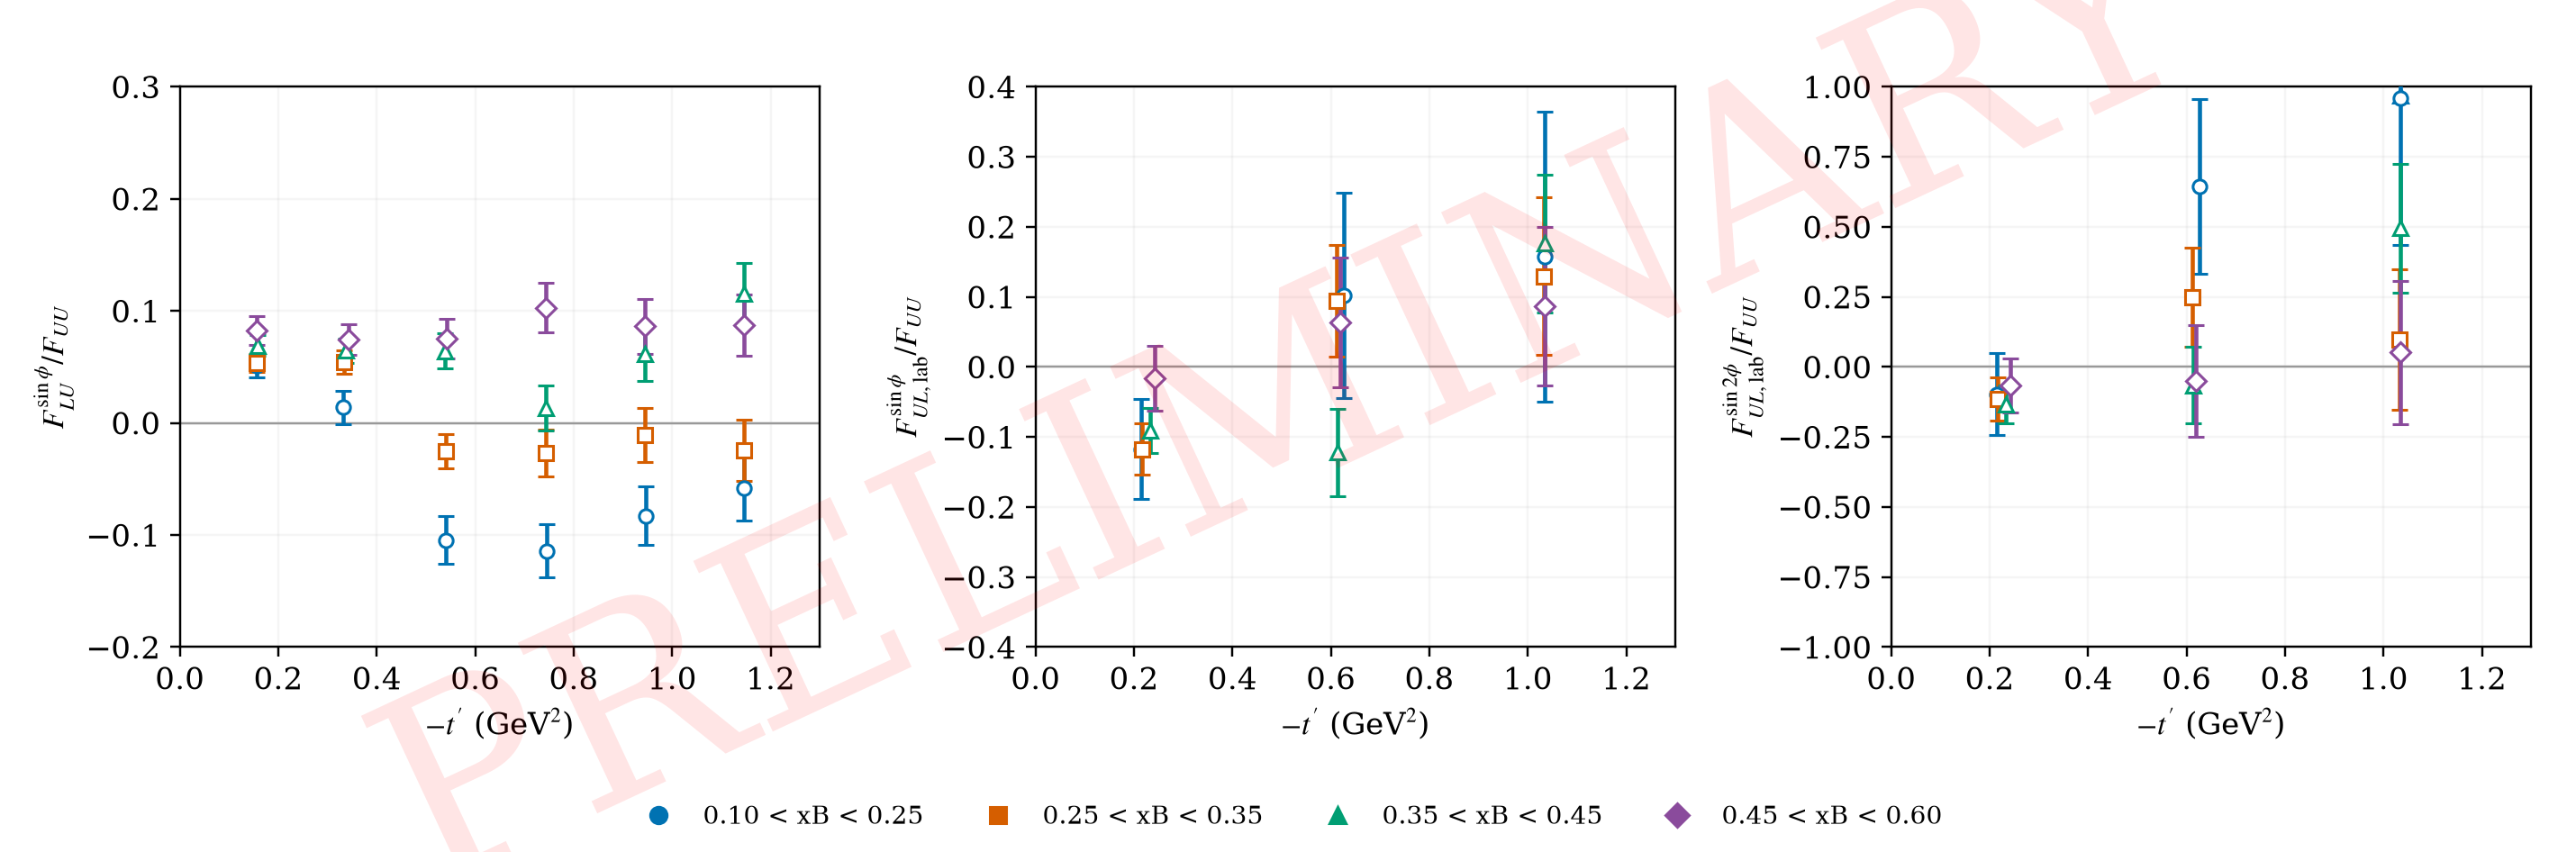
\includegraphics[width=\linewidth]{figures/results/data_overlay_all_xB.png}
\caption{Preliminary $LU$, $UL\sin\phi$ and $UL\sin2\phi$ ratios. Colors distinguish the four $x_B$ intervals. Error bars are statistical.}\label{fig:release_overlay}
\end{figure}
\clearpage
\begin{figure}[p]\centering
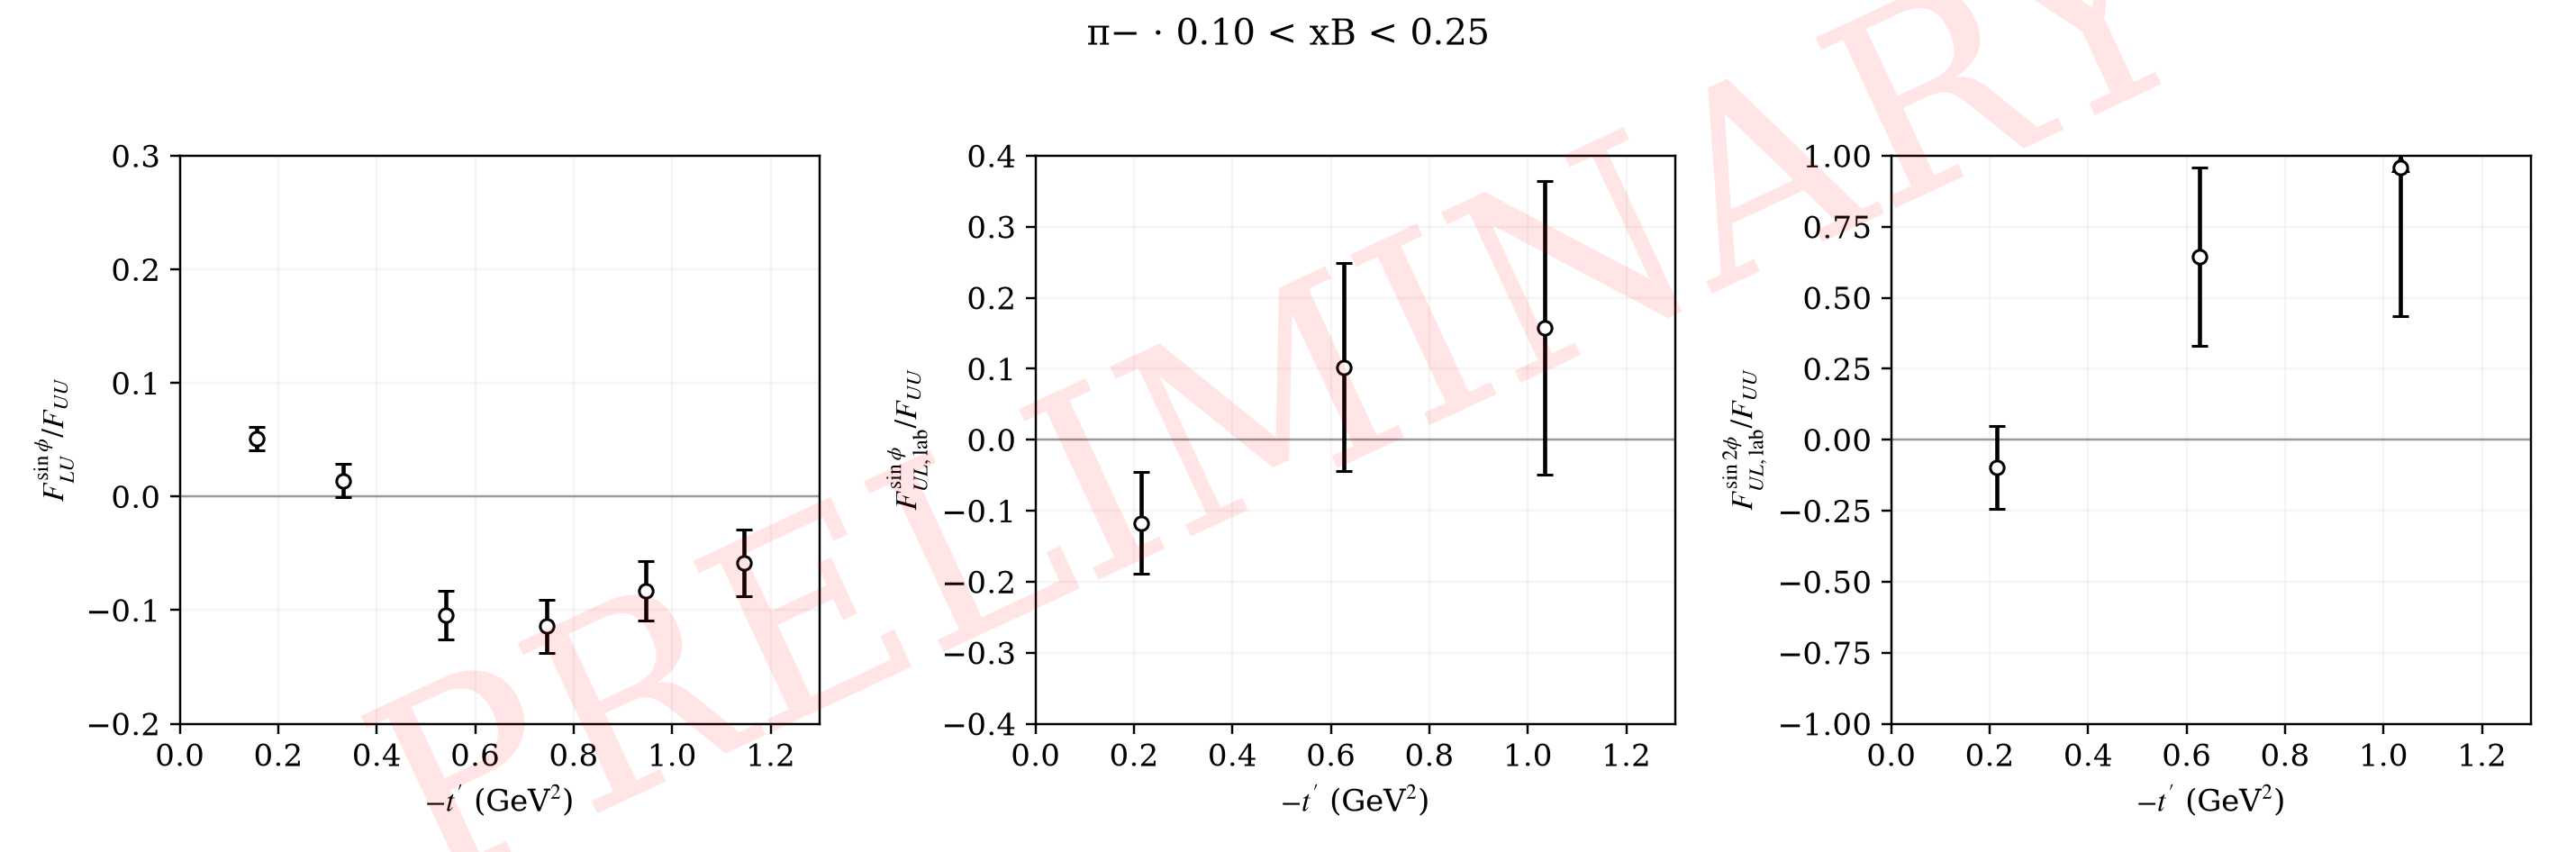
\includegraphics[width=\linewidth]{figures/results/data_xB_bin_1.png}
\caption{Preliminary spin-dependent ratios in $x_B$ interval 1. The $LU$ panel has six $-t^\prime$ bins and each $UL$ panel has three.}\label{fig:release_xb1}
\end{figure}
\clearpage
\begin{figure}[p]\centering
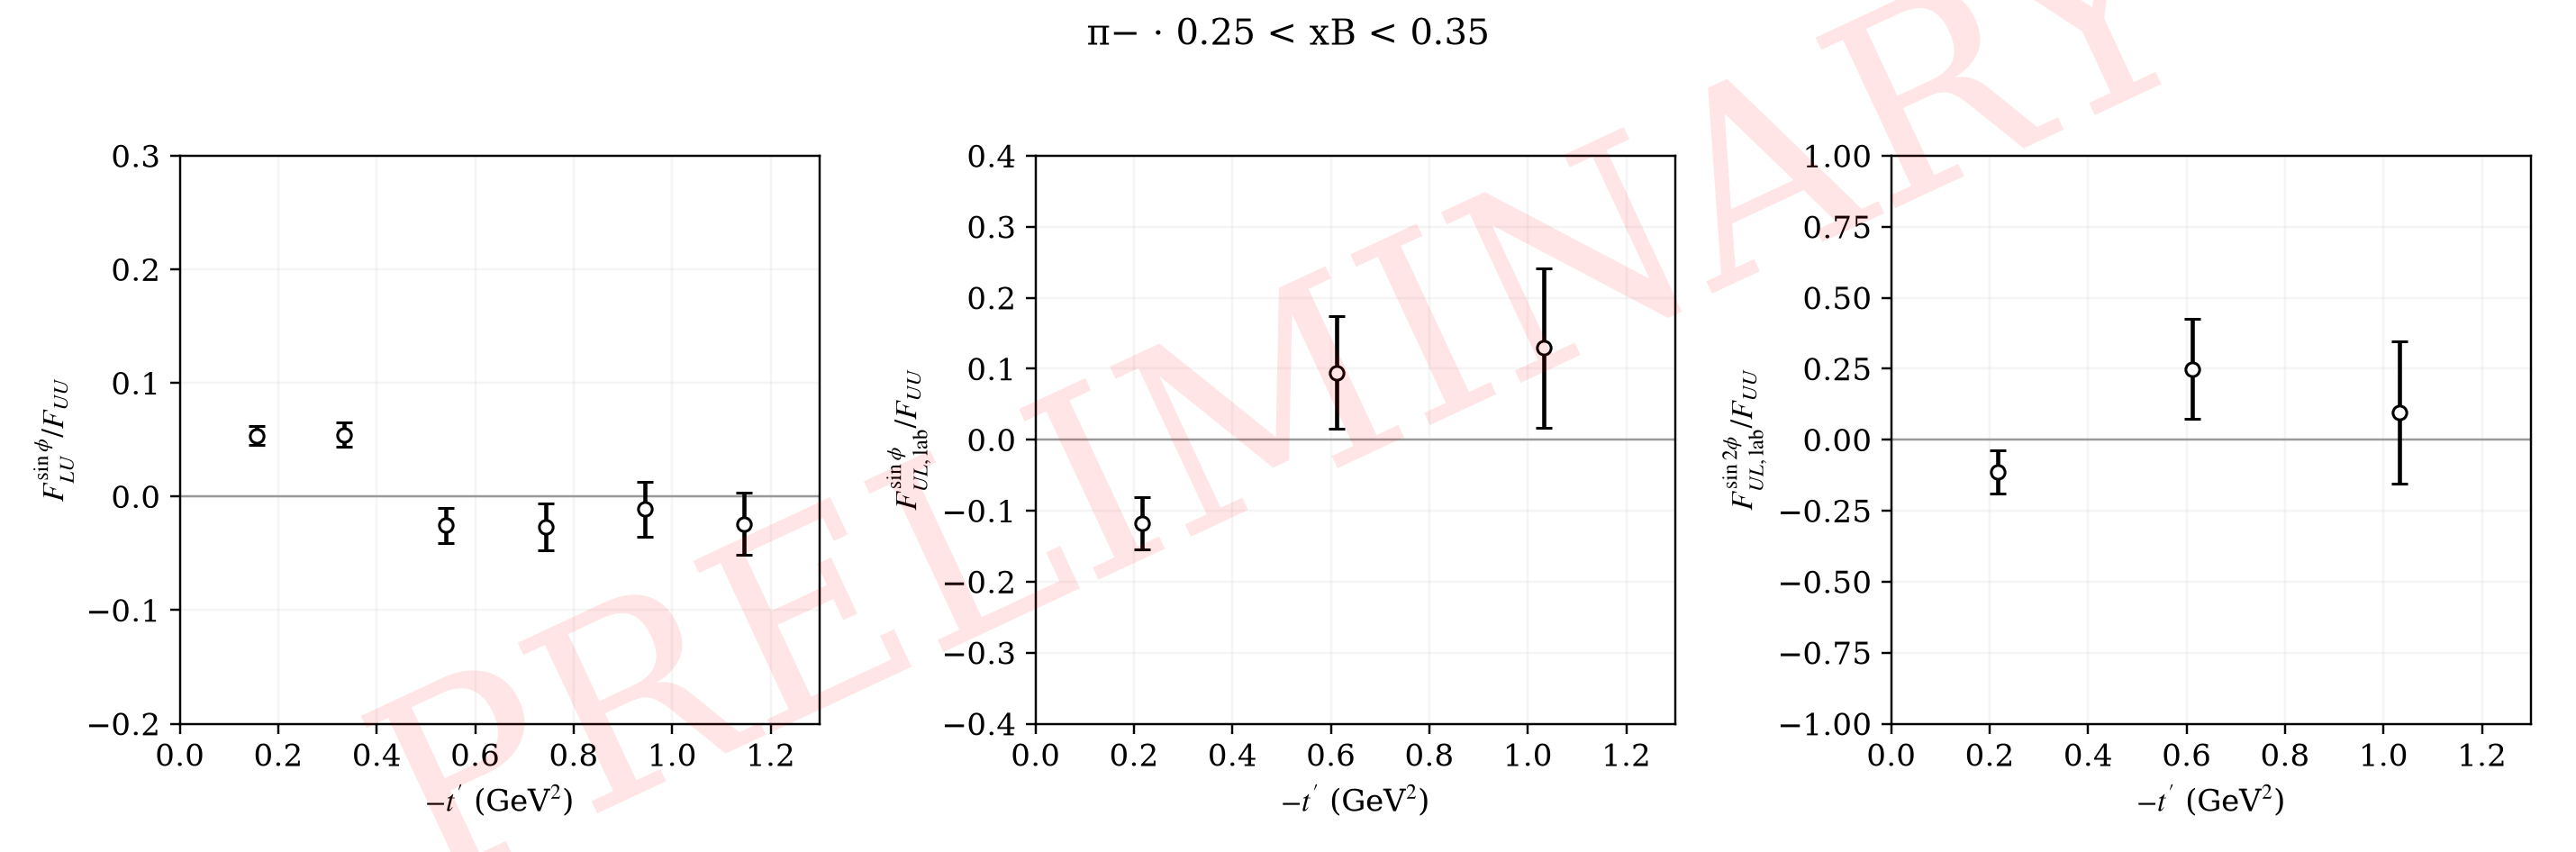
\includegraphics[width=\linewidth]{figures/results/data_xB_bin_2.png}
\caption{Preliminary spin-dependent ratios in $x_B$ interval 2. The $LU$ panel has six $-t^\prime$ bins and each $UL$ panel has three.}\label{fig:release_xb2}
\end{figure}
\clearpage
\begin{figure}[p]\centering
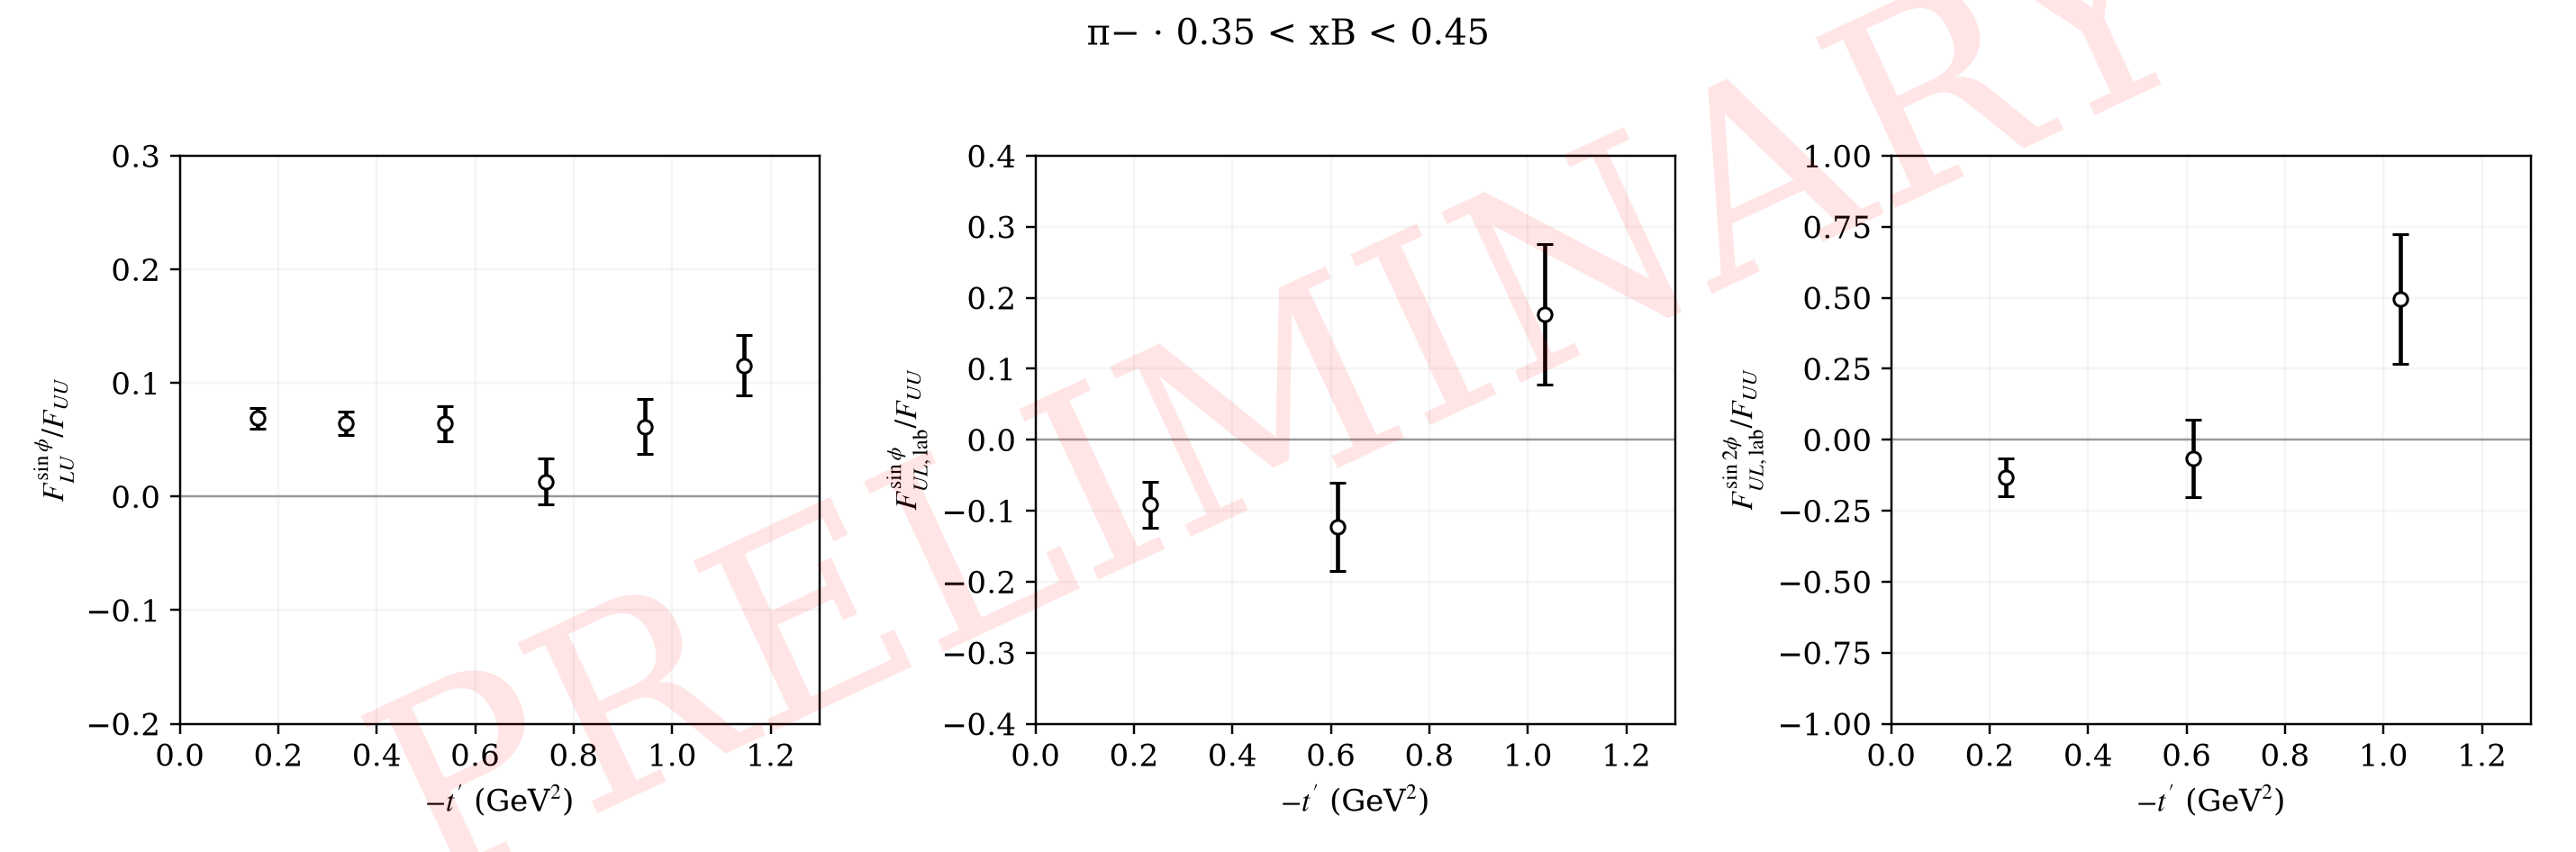
\includegraphics[width=\linewidth]{figures/results/data_xB_bin_3.png}
\caption{Preliminary spin-dependent ratios in $x_B$ interval 3. The $LU$ panel has six $-t^\prime$ bins and each $UL$ panel has three.}\label{fig:release_xb3}
\end{figure}
\clearpage
\begin{figure}[p]\centering
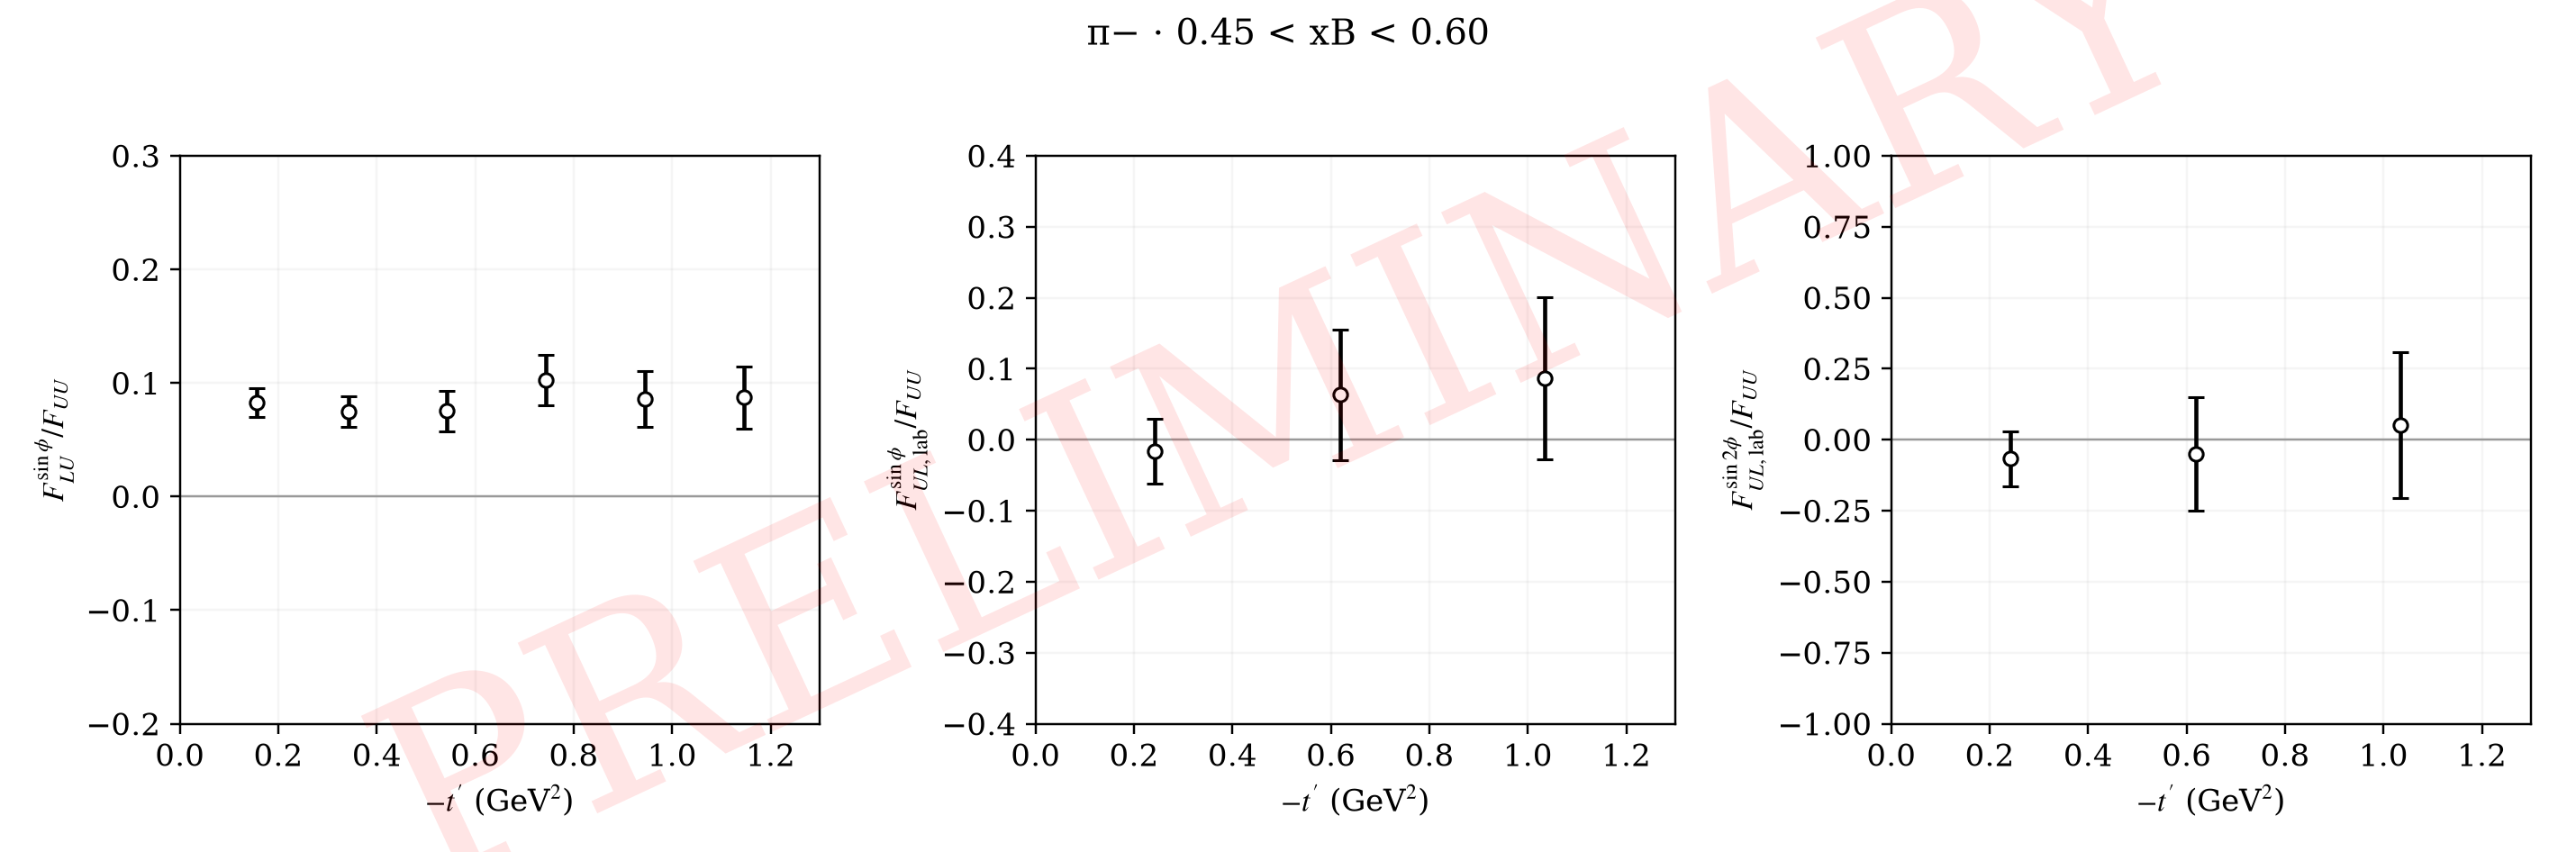
\includegraphics[width=\linewidth]{figures/results/data_xB_bin_4.png}
\caption{Preliminary spin-dependent ratios in $x_B$ interval 4. The $LU$ panel has six $-t^\prime$ bins and each $UL$ panel has three.}\label{fig:release_xb4}
\end{figure}
\clearpage

\clearpage
\begin{longtable}{rrrrr}
\caption{$F_{LU}^{\sin\phi}/F_{UU}$. Statistical uncertainties include dilution propagation where applicable.}\label{tab:release_lu1}\\
\toprule
$x_B$ interval & $-t^\prime$ interval & $\langle-t^\prime\rangle$ & Ratio & Statistical error\\
\midrule\endfirsthead
\toprule $x_B$ interval & $-t^\prime$ interval & $\langle-t^\prime\rangle$ & Ratio & Statistical error\\\midrule\endhead
0.10--0.25 & 0.05--0.25 & 0.156 & 0.0510 & 0.0100\\
0.10--0.25 & 0.25--0.45 & 0.332 & 0.0139 & 0.0146\\
0.10--0.25 & 0.45--0.65 & 0.541 & -0.1045 & 0.0213\\
0.10--0.25 & 0.65--0.85 & 0.745 & -0.1142 & 0.0236\\
0.10--0.25 & 0.85--1.05 & 0.947 & -0.0828 & 0.0260\\
0.10--0.25 & 1.05--1.25 & 1.146 & -0.0582 & 0.0292\\
0.25--0.35 & 0.05--0.25 & 0.157 & 0.0538 & 0.0080\\
0.25--0.35 & 0.25--0.45 & 0.333 & 0.0546 & 0.0105\\
0.25--0.35 & 0.45--0.65 & 0.540 & -0.0253 & 0.0155\\
0.25--0.35 & 0.65--0.85 & 0.743 & -0.0267 & 0.0208\\
0.25--0.35 & 0.85--1.05 & 0.945 & -0.0110 & 0.0241\\
0.25--0.35 & 1.05--1.25 & 1.146 & -0.0241 & 0.0273\\
0.35--0.45 & 0.05--0.25 & 0.158 & 0.0691 & 0.0090\\
0.35--0.45 & 0.25--0.45 & 0.338 & 0.0644 & 0.0106\\
0.35--0.45 & 0.45--0.65 & 0.539 & 0.0641 & 0.0156\\
0.35--0.45 & 0.65--0.85 & 0.743 & 0.0133 & 0.0201\\
0.35--0.45 & 0.85--1.05 & 0.945 & 0.0617 & 0.0244\\
0.35--0.45 & 1.05--1.25 & 1.146 & 0.1156 & 0.0268\\
0.45--0.60 & 0.05--0.25 & 0.156 & 0.0825 & 0.0126\\
0.45--0.60 & 0.25--0.45 & 0.343 & 0.0745 & 0.0135\\
0.45--0.60 & 0.45--0.65 & 0.543 & 0.0754 & 0.0178\\
0.45--0.60 & 0.65--0.85 & 0.744 & 0.1028 & 0.0222\\
0.45--0.60 & 0.85--1.05 & 0.946 & 0.0861 & 0.0246\\
0.45--0.60 & 1.05--1.25 & 1.146 & 0.0874 & 0.0274\\
\bottomrule
\end{longtable}


\clearpage
\begin{longtable}{rrrrr}
\caption{$F_{UL,\mathrm{lab}}^{\sin\phi}/F_{UU}$. Statistical uncertainties include dilution propagation where applicable.}\label{tab:release_ul1}\\
\toprule
$x_B$ interval & $-t^\prime$ interval & $\langle-t^\prime\rangle$ & Ratio & Statistical error\\
\midrule\endfirsthead
\toprule $x_B$ interval & $-t^\prime$ interval & $\langle-t^\prime\rangle$ & Ratio & Statistical error\\\midrule\endhead
0.10--0.25 & 0.05--0.45 & 0.214 & -0.1174 & 0.0715\\
0.10--0.25 & 0.45--0.85 & 0.626 & 0.1023 & 0.1462\\
0.10--0.25 & 0.85--1.25 & 1.034 & 0.1576 & 0.2070\\
0.25--0.35 & 0.05--0.45 & 0.216 & -0.1174 & 0.0368\\
0.25--0.35 & 0.45--0.85 & 0.611 & 0.0947 & 0.0795\\
0.25--0.35 & 0.85--1.25 & 1.032 & 0.1294 & 0.1125\\
0.35--0.45 & 0.05--0.45 & 0.232 & -0.0912 & 0.0323\\
0.35--0.45 & 0.45--0.85 & 0.613 & -0.1221 & 0.0621\\
0.35--0.45 & 0.85--1.25 & 1.034 & 0.1765 & 0.0986\\
0.45--0.60 & 0.05--0.45 & 0.241 & -0.0160 & 0.0460\\
0.45--0.60 & 0.45--0.85 & 0.618 & 0.0636 & 0.0921\\
0.45--0.60 & 0.85--1.25 & 1.034 & 0.0867 & 0.1137\\
\bottomrule
\end{longtable}


\clearpage
\begin{longtable}{rrrrr}
\caption{$F_{UL,\mathrm{lab}}^{\sin2\phi}/F_{UU}$. Statistical uncertainties include dilution propagation where applicable.}\label{tab:release_ul2}\\
\toprule
$x_B$ interval & $-t^\prime$ interval & $\langle-t^\prime\rangle$ & Ratio & Statistical error\\
\midrule\endfirsthead
\toprule $x_B$ interval & $-t^\prime$ interval & $\langle-t^\prime\rangle$ & Ratio & Statistical error\\\midrule\endhead
0.10--0.25 & 0.05--0.45 & 0.214 & -0.0969 & 0.1465\\
0.10--0.25 & 0.45--0.85 & 0.626 & 0.6444 & 0.3133\\
0.10--0.25 & 0.85--1.25 & 1.034 & 0.9739 & 0.5240\\
0.25--0.35 & 0.05--0.45 & 0.216 & -0.1139 & 0.0762\\
0.25--0.35 & 0.45--0.85 & 0.611 & 0.2498 & 0.1774\\
0.25--0.35 & 0.85--1.25 & 1.032 & 0.0965 & 0.2509\\
0.35--0.45 & 0.05--0.45 & 0.232 & -0.1327 & 0.0672\\
0.35--0.45 & 0.45--0.85 & 0.613 & -0.0648 & 0.1360\\
0.35--0.45 & 0.85--1.25 & 1.034 & 0.4950 & 0.2285\\
0.45--0.60 & 0.05--0.45 & 0.241 & -0.0666 & 0.0976\\
0.45--0.60 & 0.45--0.85 & 0.618 & -0.0501 & 0.1992\\
0.45--0.60 & 0.85--1.25 & 1.034 & 0.0513 & 0.2567\\
\bottomrule
\end{longtable}

The period comparisons retain separate likelihood normalizations and the common dilution convention. They are diagnostic comparisons of samples with different within-bin kinematic populations. Across the tested BM-fixed scenarios, the largest changes in $UL\sin\phi$ and $UL\sin2\phi$ are 0.071 and 0.047 times the free-fit statistical error, respectively. The errors themselves are essentially unchanged. These are paired-fit sensitivity scales, not significances. The free baseline is therefore retained without a model constraint on $LL\cos\phi$.
\begin{figure}[p]\centering
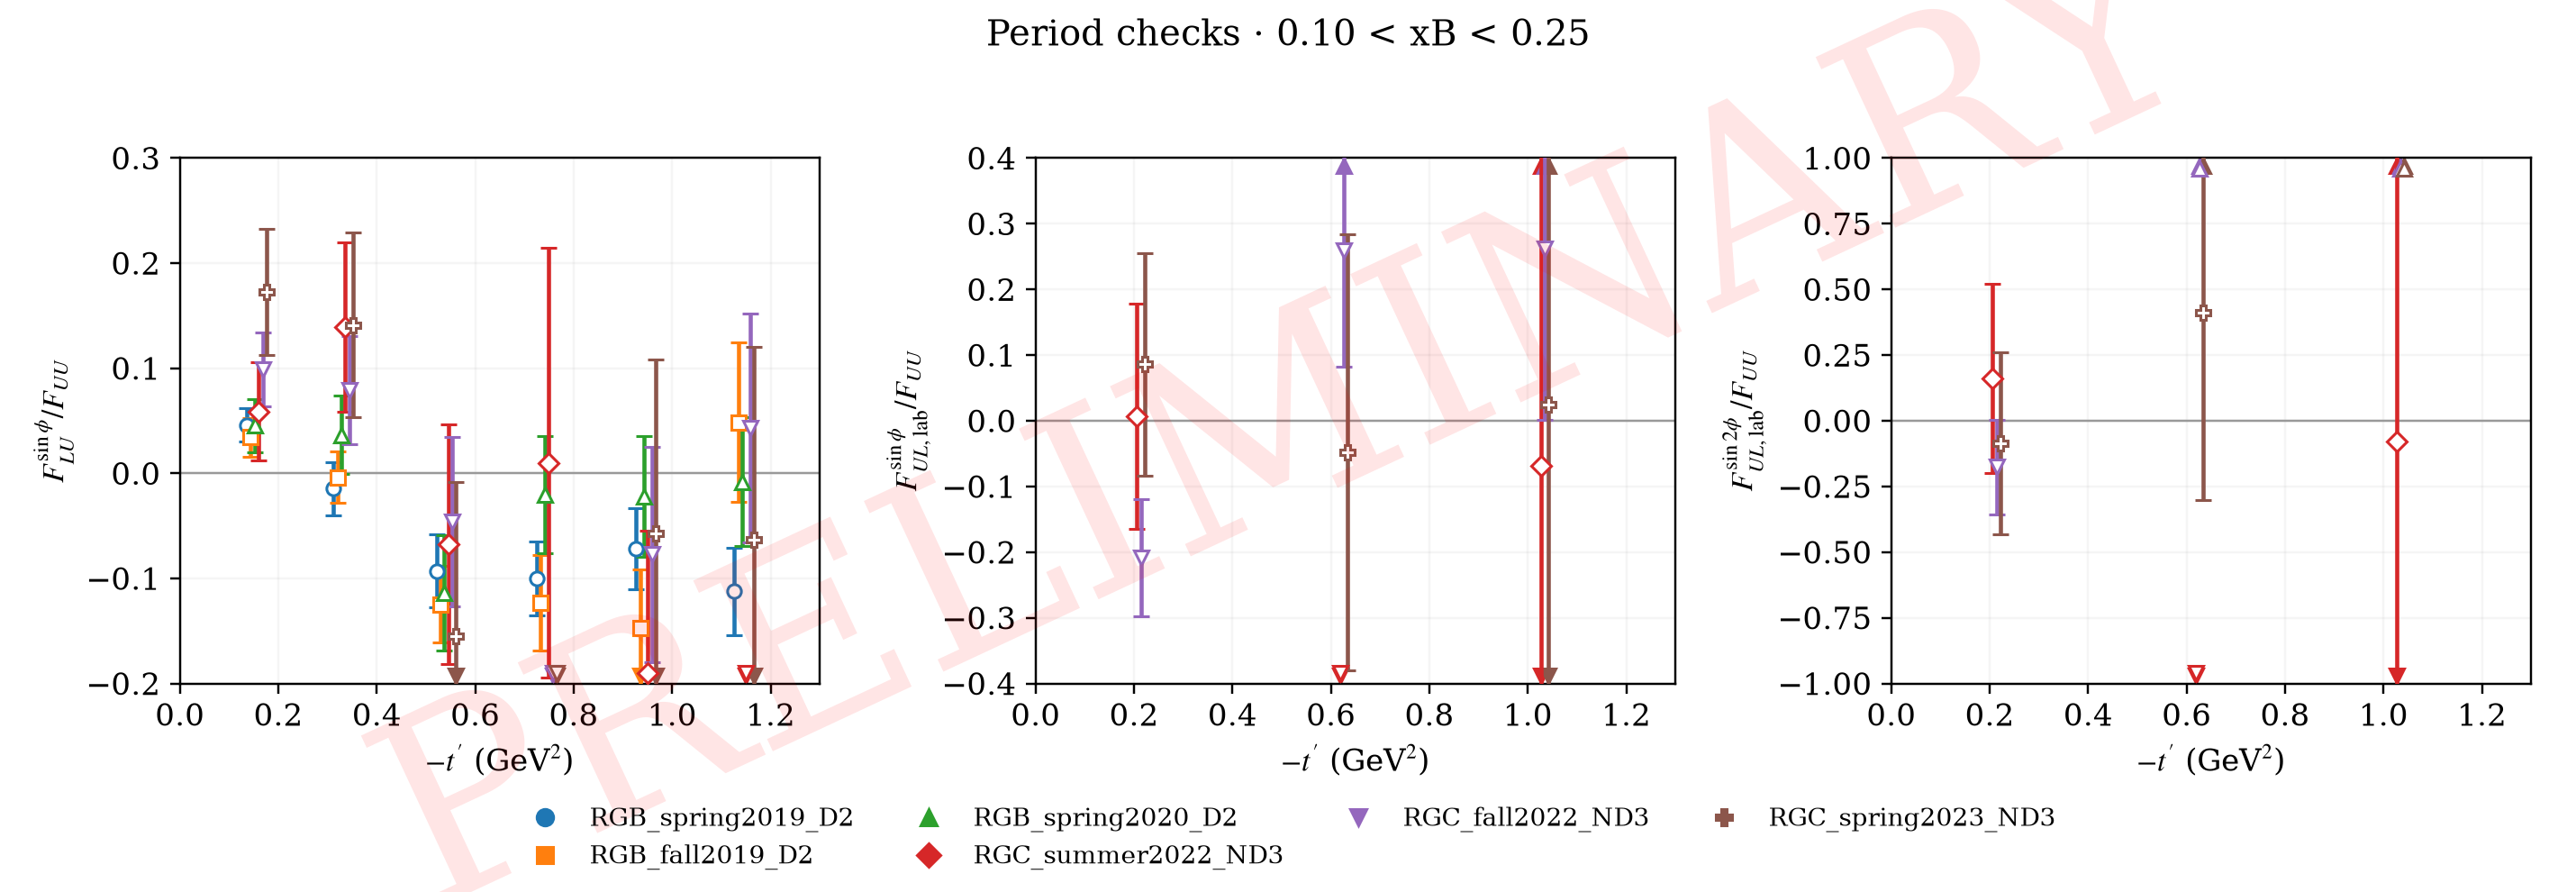
\includegraphics[width=\linewidth]{figures/results/periods_xB_bin_1.png}
\caption{Period comparison in $x_B$ interval 1. $LU$ includes the three RGB and three RGC samples; the target-spin panels show the three RGC ND$_3$ periods. Points are displaced horizontally for readability. Shared dilution uncertainties correlate target-period results.}\label{fig:release_period1}
\end{figure}
\clearpage
\begin{figure}[p]\centering
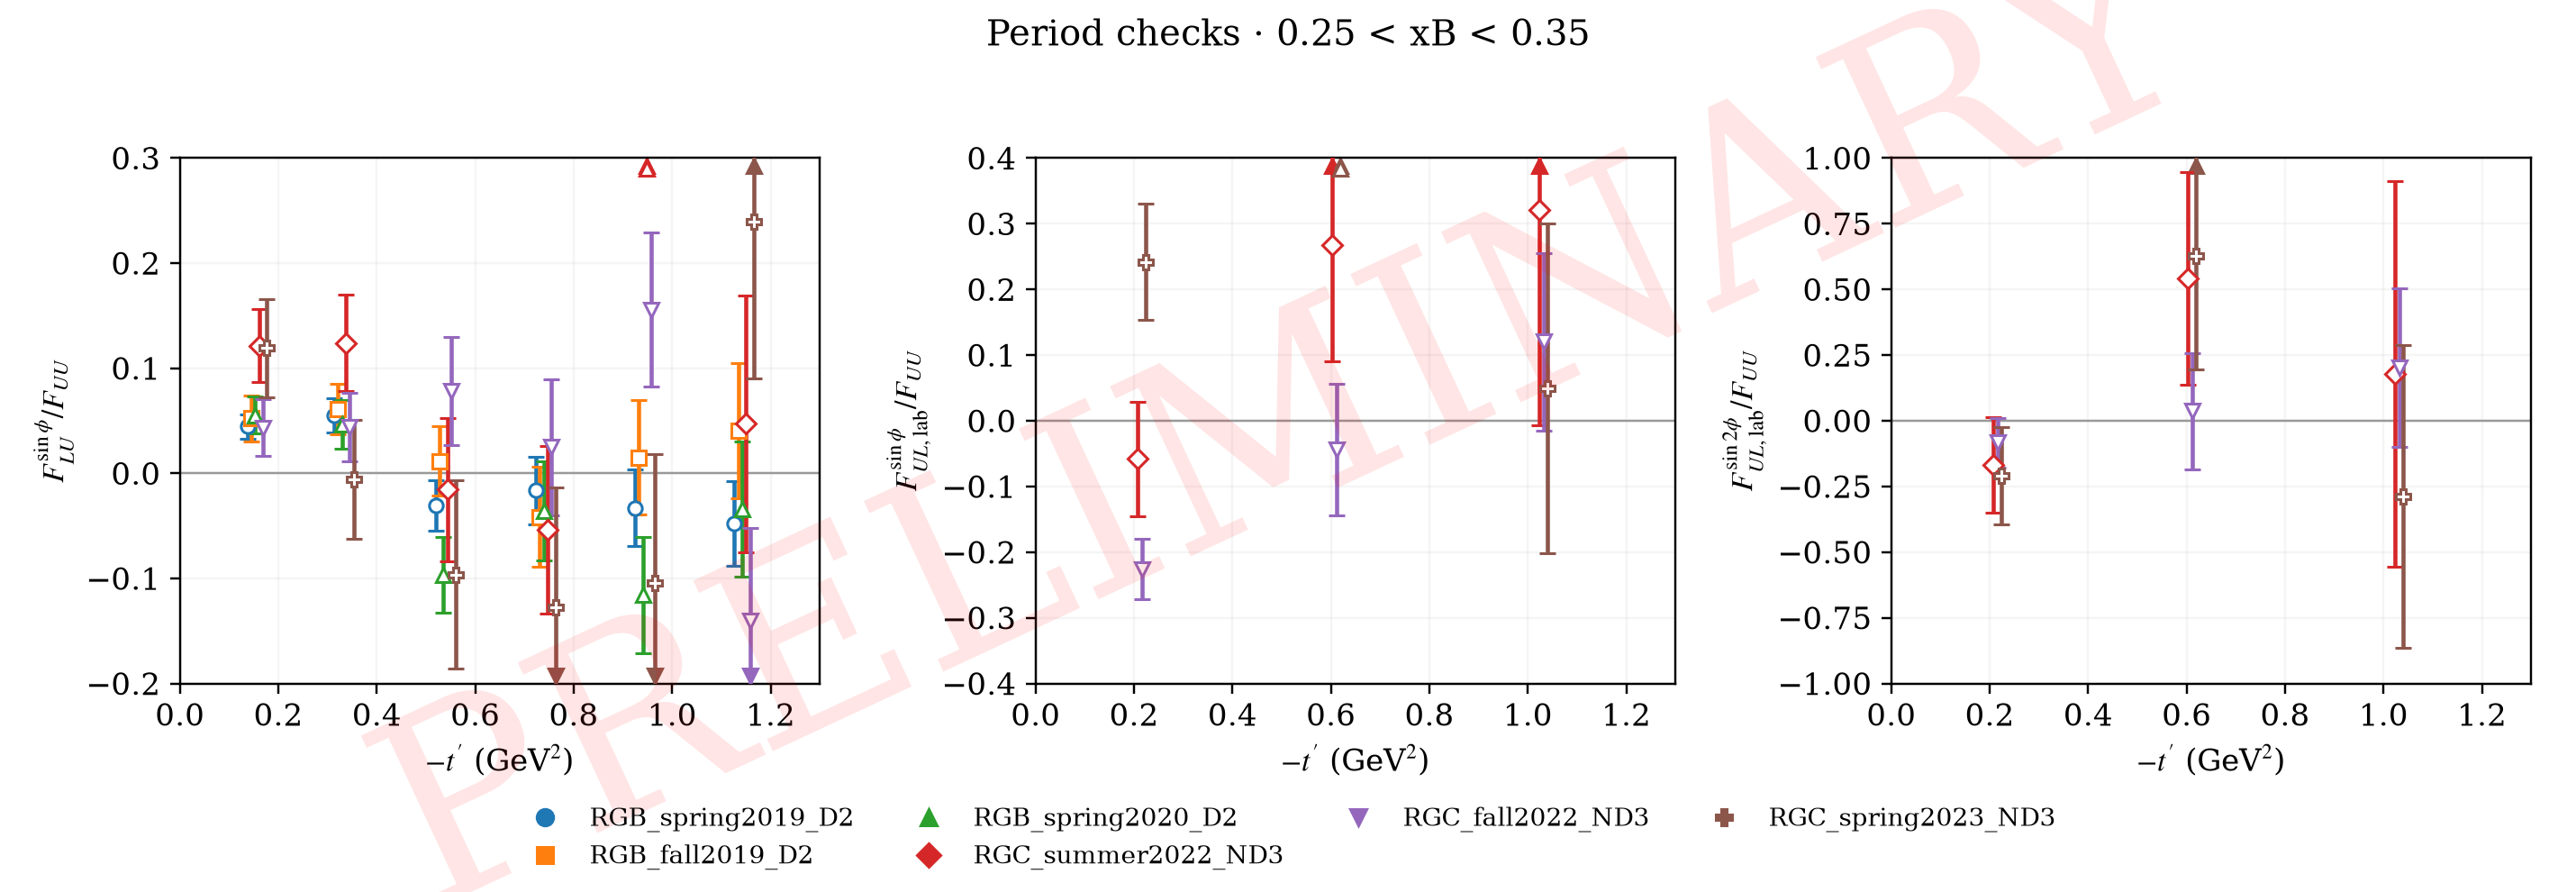
\includegraphics[width=\linewidth]{figures/results/periods_xB_bin_2.png}
\caption{Period comparison in $x_B$ interval 2. $LU$ includes the three RGB and three RGC samples; the target-spin panels show the three RGC ND$_3$ periods. Points are displaced horizontally for readability. Shared dilution uncertainties correlate target-period results.}\label{fig:release_period2}
\end{figure}
\clearpage
\begin{figure}[p]\centering
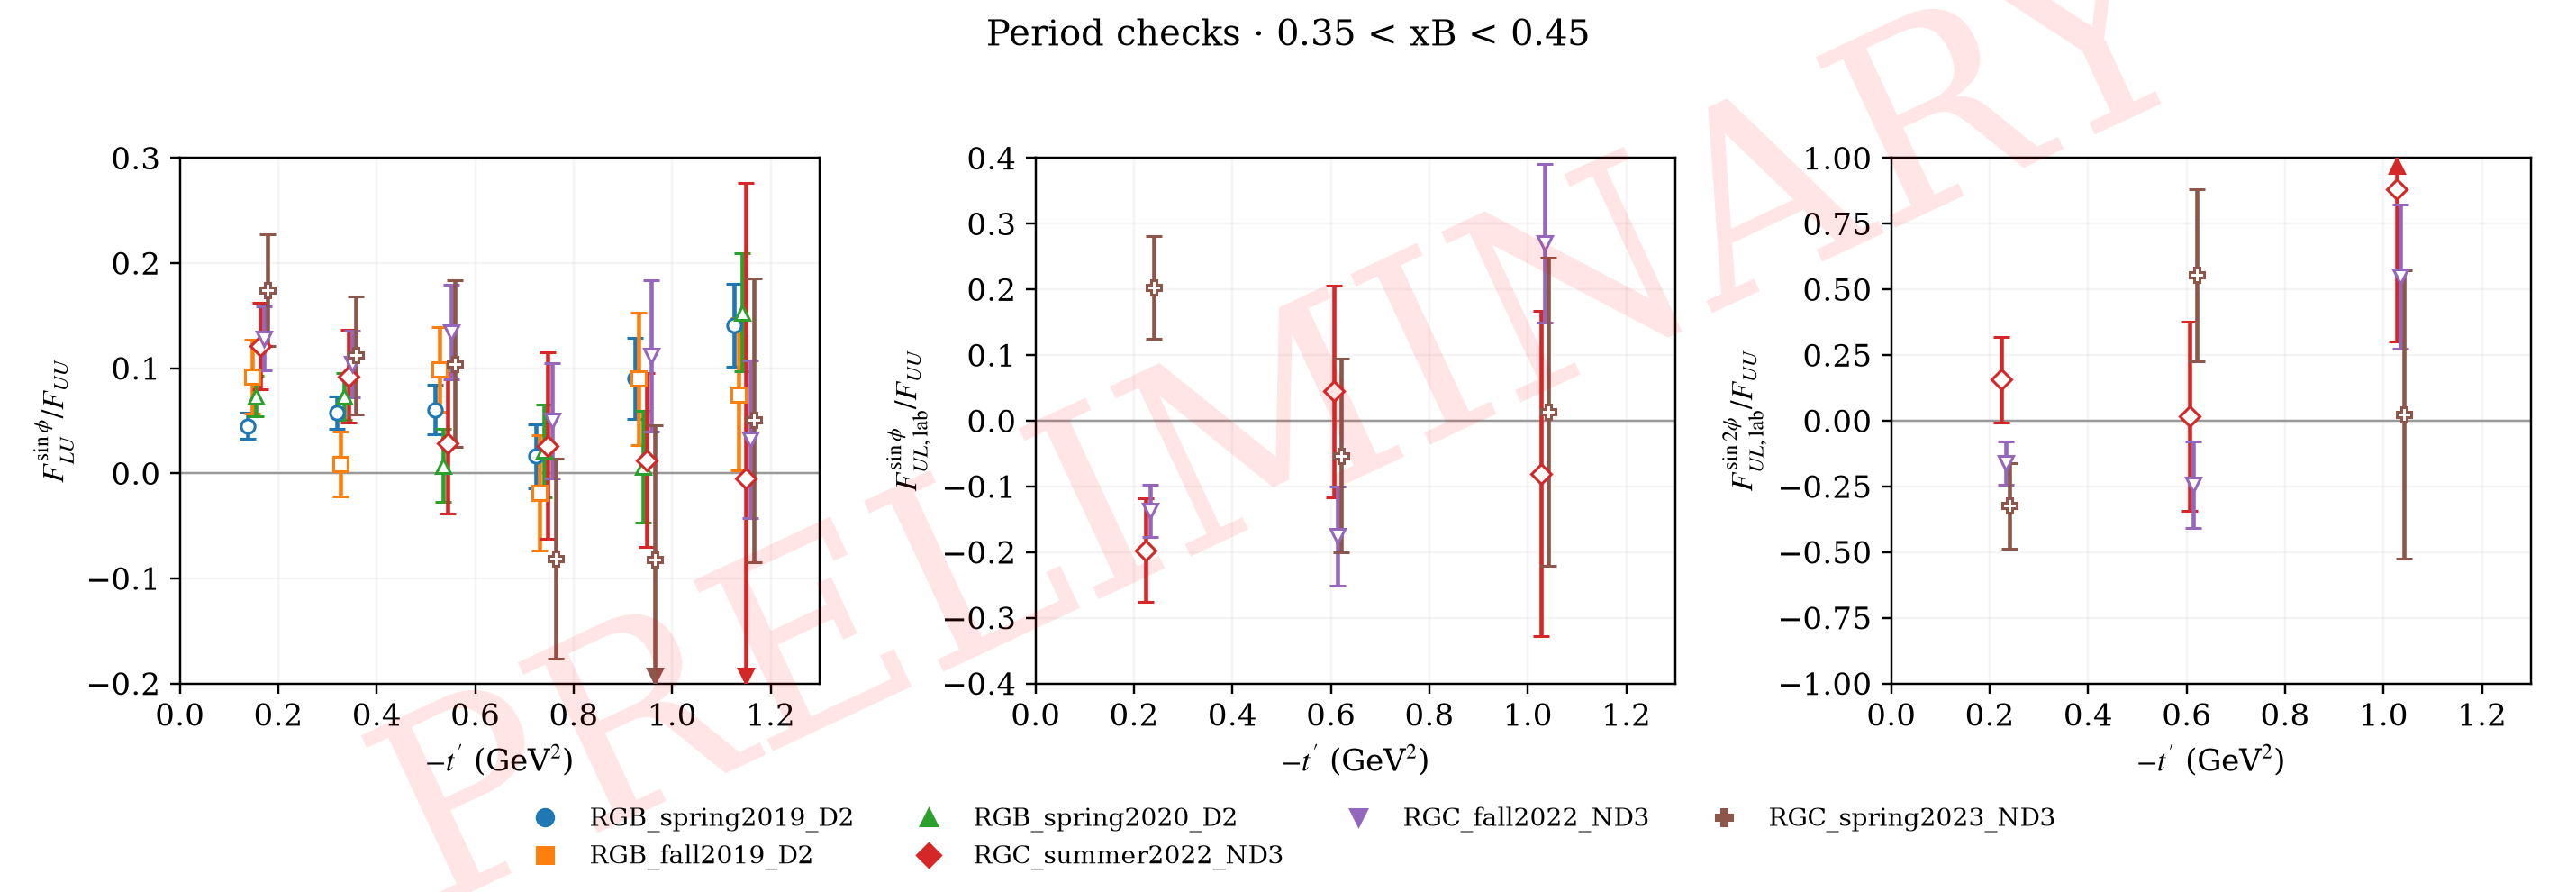
\includegraphics[width=\linewidth]{figures/results/periods_xB_bin_3.png}
\caption{Period comparison in $x_B$ interval 3. $LU$ includes the three RGB and three RGC samples; the target-spin panels show the three RGC ND$_3$ periods. Points are displaced horizontally for readability. Shared dilution uncertainties correlate target-period results.}\label{fig:release_period3}
\end{figure}
\clearpage
\begin{figure}[p]\centering
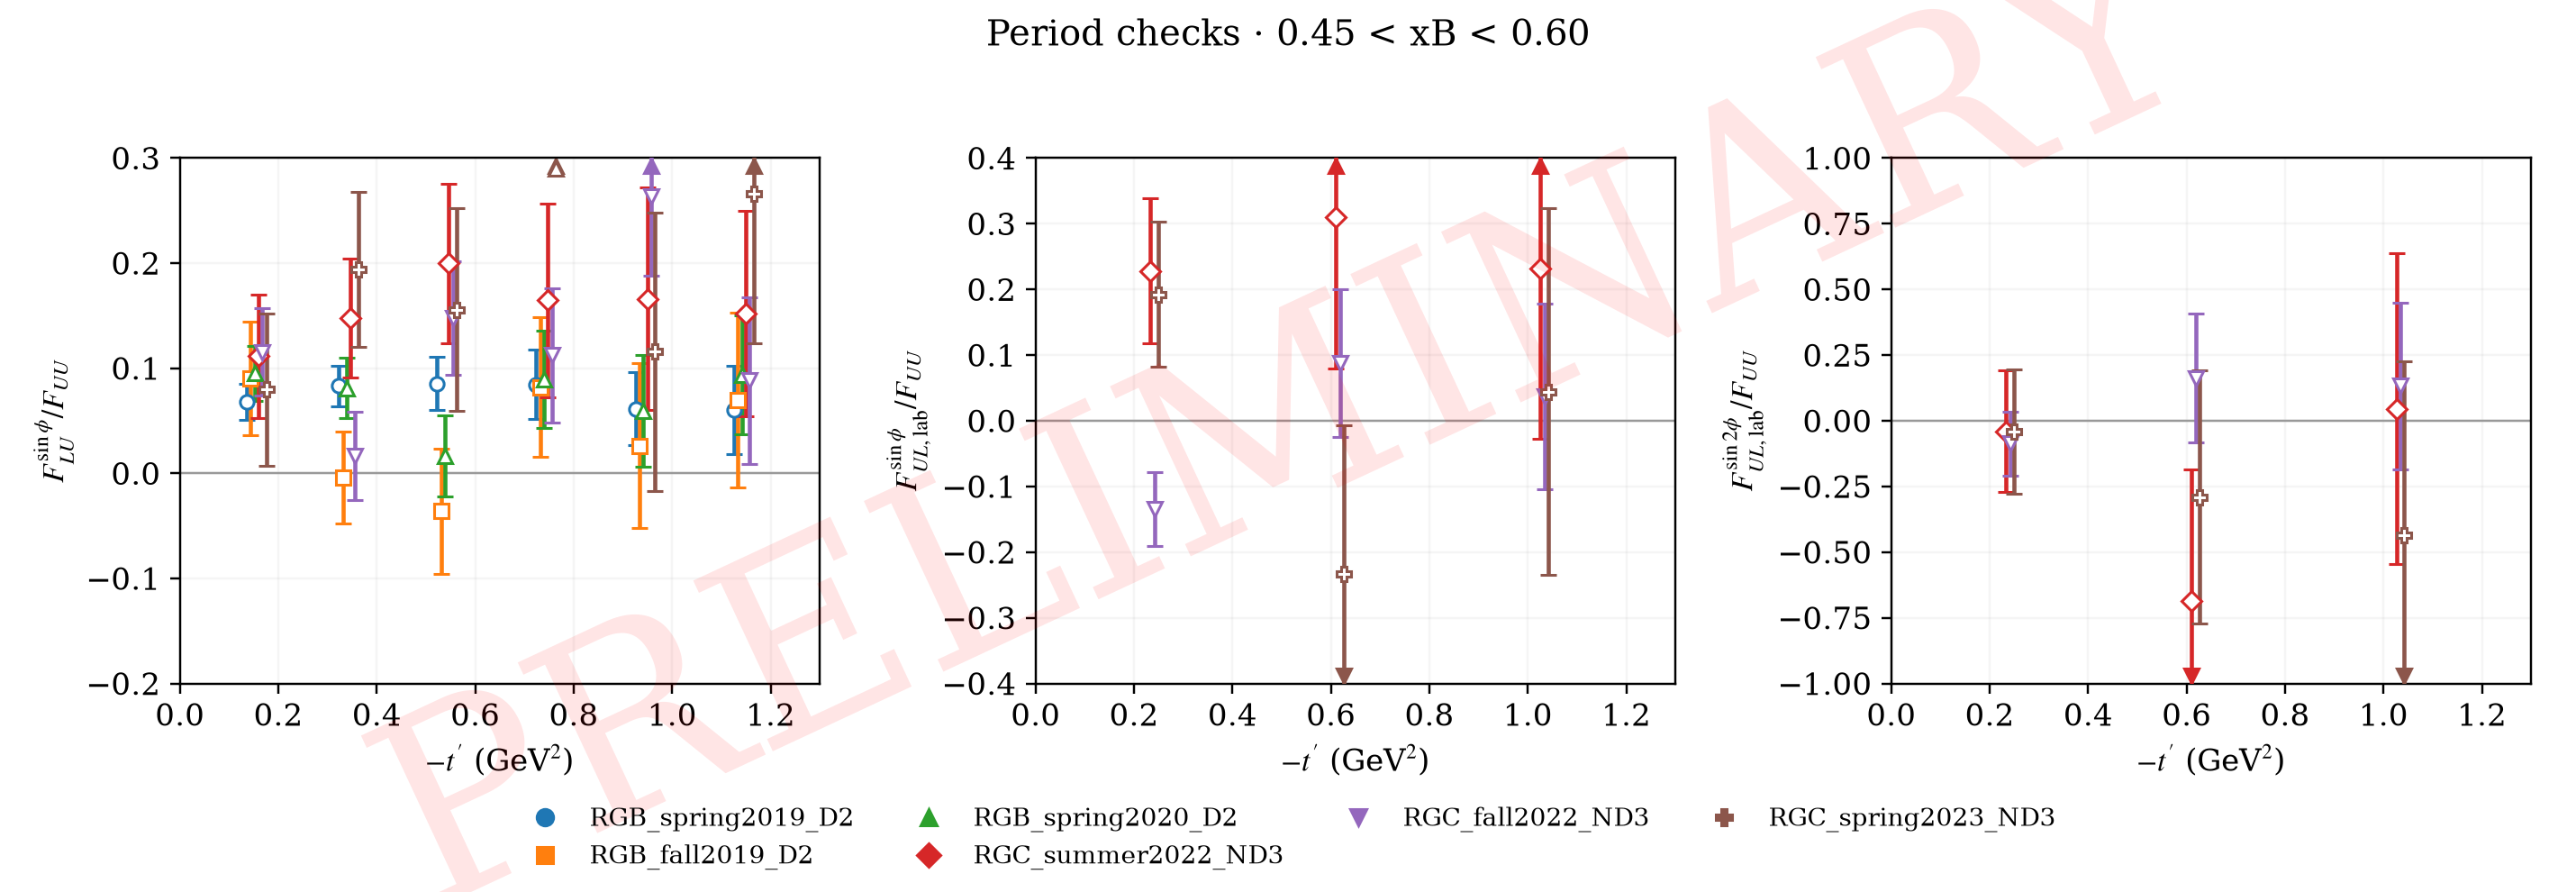
\includegraphics[width=\linewidth]{figures/results/periods_xB_bin_4.png}
\caption{Period comparison in $x_B$ interval 4. $LU$ includes the three RGB and three RGC samples; the target-spin panels show the three RGC ND$_3$ periods. Points are displaced horizontally for readability. Shared dilution uncertainties correlate target-period results.}\label{fig:release_period4}
\end{figure}
\clearpage

\subsection{Comparison to Manley--Bhattacharya Predictions}\label{sec:mb_comparison}
The Manley--Bhattacharya (MB) calculation combines leading-twist longitudinal amplitudes involving $\widetilde H$ and $\widetilde E$, including the charged-pion pole, with transverse amplitudes at twist~3. The transverse sector contains both the chiral-odd $H_T$ and $\bar E_T$ contributions coupled to a twist-3 pion distribution amplitude, and additional chiral-even contributions from moments of generalized transverse-momentum dependent distributions (GTMDs) coupled to a twist-2 pion distribution amplitude. In the supplied implementation, endpoint integrals are regulated with $\delta=\langle p_\perp^2\rangle/Q^2$; separate chiral-even and chiral-odd regulator parameters and a transversity $t$ slope are fitted to CLAS6 unpolarized $\pi^0$ cross sections. The displayed theory bands propagate the parameter-fit uncertainty, rather than representing the full model uncertainty.
The description above summarizes preliminary theory material supplied for the $\pi^+$ comparison; numerical neutron-channel predictions and their kinematic evaluation must be supplied and checked before any curves are shown here. The published GK framework instead describes longitudinal amplitudes with $\widetilde H$, $\widetilde E$ and the charged-pion pole, and important transverse amplitudes with chiral-odd GPDs and a twist-3 pion wave function~\cite{Goloskokov:2009ia,Goloskokov:2011rd}. The additional chiral-even GTMD-moment contributions in the MB treatment provide a distinct mechanism to examine in the transverse cross section. The comparison will retain the measured lab-axis convention, finite-bin kinematics, polarization definitions, and the distinction between parameter-fit bands and full model uncertainty. No numerical agreement or disagreement is claimed at this stage.
% Add neutron-channel predictions, figures and results after extraction.


\clearpage\bibliographystyle{ieeetr}\bibliography{references}
\end{document}
